%; whizzy paragraph
%; whizzy-paragraph "^\\\\dancersection"
% -initex iniptex -latex platex -format platex -bibtex jbibtex -fmt fmt
% $B0J>e(B whizzytex $B$r;HMQ$9$k>l9g$N@_Dj!#(B

%     Tokyo Debian Meeting resources
%     Kansai Debian Meeting resources
%     Copyright (C) 2008 Junichi Uekawa
%     Copyright (C) 2008 Nobuhiro Iwamatsu

%     This program is free software; you can redistribute it and/or modify
%     it under the terms of the GNU General Public License as published by
%     the Free Software Foundation; either version 2 of the License, or
%     (at your option) any later version.

%     This program is distributed in the hope that it will be useful,
%     but WITHOUT ANY WARRANTY; without even the implied warranty of
%     MERCHANTABILITY or FITNESS FOR A PARTICULAR PURPOSE.  See the
%     GNU General Public License for more details.

%     You should have received a copy of the GNU General Public License
%     along with this program; if not, write to the Free Software
%     Foundation, Inc., 51 Franklin St, Fifth Floor, Boston, MA  02110-1301 USA

%   Pdf$B:n@.<j=g(B
% dvipdfmx debianmeetingresume200606.dvi
%  preview (shell-command (concat "evince " (replace-regexp-in-string "tex$" "pdf"(buffer-file-name)) "&"))
% $B2hA|%U%!%$%k$r=hM}$9$k$?$a$K$O(Bebb$B$rMxMQ$7$F(Bboundingbox$B$r:n@.!#(B
%(shell-command "cd image2007-fuyu; ebb *.png")


% progress memo: 
% 2008/12-2009/5$B$,%^!<%8BP>]!"4X@>$O(B2008/12-2009/5
% $B%$%Y%s%HEy$G$J$$>l9g$OM}M3$r=q$/$3$H!#(B
% $BI,MW$JJQ99E@$O(B FIXME $B$G5-O?$7$F$$$^$9!#(B

%%$B$3$3$+$i%X%C%@3+;O!#(B

\documentclass[mingoth,a4paper]{jsarticle}
\usepackage{monthlyreport}
\usepackage[dvips]{xy} % for advi workaround. Bug #452044

% section $B$NBe$o$j$N4D6-(B -- $B2~D{$9$k!#(B
\renewcommand{\dancersection}[2]{%
\newpage
$B$"$s$I$-$e$a$s$F$C$I(B $B$G$S$"$s(B 2009$BG/2F9f(B
%
% top line
\vspace{0.1mm}\\
{\color{dancerlightblue}\rule{\hsize}{2mm}}

%
% middle text
%
\begin{minipage}[t]{0.6\hsize}
\color{dancerdarkblue}
\vspace{1cm}
\section{#1}
\hfill{}#2\\
\end{minipage}
\begin{minipage}[t]{0.4\hsize}
\vspace{-2cm}
\hfill{}
\includegraphics[height=8cm]{image200502/openlogo-nd.eps}\\
\vspace{-5cm}
\end{minipage}
%
%
{\color{dancerdarkblue}\rule{0.74\hsize}{2mm}}
%
\vspace{2cm}
}


\begin{document}
\begin{titlepage}
\includegraphics[height=252mm]{image2009-natsu/2009-summer.eps}
%\thispagestyle{empty}
\end{titlepage}

\newpage
\begin{minipage}[]{0.2\hsize}
 \definecolor{titleback}{gray}{0.9}
 \colorbox{dancerlightblue}{\rotatebox{90}{\fontsize{80}{80} 
{\gt \color{dancerdarkblue}$B%G%S%"%sJY6/2q(B} }}
\end{minipage}
\begin{minipage}[]{0.8\hsize}
\hrule
\vspace{1mm}
\hrule
\setcounter{tocdepth}{1}
{\small
 \tableofcontents}
\vspace{1mm}
\hrule
\vspace{3cm}

\end{minipage}

% FIXME: $BK\J8$rDI2C$9$k$3$H!#(B
% from debianmeetingresume200812.tex
\dancersection{Introduction}{$B>e@n(B $B=c0l(B}
 
 Debian$BJY6/2q$X$h$&$3$=!#$3$l$+$i(BDebian$B$N@$3&$K$"$7$rF'$_F~$l$k$H(B
 $B$$$&J}$b!"$9$G$K$I$C$W$j$H$D$+$C$F$$$k$H$$$&J}$b!"7n$K0l2s(BDebian$B$K$D$$(B
 $B$F8l$j$^$;$s$+!)(B

 Debian$BJY6/2q$NL\E*$O2<5-$G$9!#(B

\begin{itemize}
 \item \underline{Debian Developer} ($B3+H/<T(B)$B$N0i@.!#(B
 \item $BF|K\8l$G$N!V(B\underline{$B3+H/$K4X$9$k>pJs(B}$B!W$r@0M}$7$F$^$H$a!"%"%C%W%G!<%H$9$k!#(B
 \item \underline{$B>l(B}$B$NDs6!!#(B
 \begin{itemize}
  \item $BIaCJ$P$i$P$i$J>l=j$K$$$k?M!9$,(B face-to-face $B$G=P2q$($k>l$rDs6!(B
	$B$9$k!#(B
  \item Debian $B$N$?$a$K$J$k$3$H$r8l$k>l$rDs6!$9$k!#(B
  \item Debian$B$K$D$$$F8l$k>l$rDs6!$9$k!#(B
 \end{itemize}
\end{itemize}		

 Debian$B$NJY6/2q$H$$$&$3$H$G5f6KE*$K$O;22C<TA40w$,(BDebian Package$B$r$,$j$,$j(B
 $B$H:n$k%9!<%Q!<%O%C%+!<$K$J$C$?;Q$rLQA[$7$F$$$^$9!#>pJs$N6&M-!&3hMQ$rDL$7(B
 $B$F(B Debian$B$N:#8e$NG=F0E*$JE83+$X$NEZBf$H$7$F!"!V>l!W$H$7$F$N6u4V$rDs6!$9(B
 $B$k$N$,L\E*$G$9!#(B

\dancersection{$B3F<o%$%Y%s%H3+:E<B@S(B}{$B>e@n(B $B=c0l(B}
\label{sec:debmtg2008results}
\index{debianjp@Debian JP} 
\index{$B$H$&$-$g$&$($j$"(B@$BEl5~%(%j%"(BDebian$BJY6/2q(B}

Debian $B3+H/<T$N0i@.$rL\E*$H$7$F3+:E$7$F$-$?El5~%(%j%"(BDebian$BJY6/2q$b:#2s(B
$B$G(B4$BG/L\$,=*N;$7$^$7$?!#(B
$B;vA02]Bj;v8e2]Bj$r@_Dj$7$F$*$j!"M==,I|=,$rI,MW$@$H$&$?$C$F$$$kJY6/2q$G$9(B
$B$,!"<B:]$K$I$l$/$i$$<B;\$5$l$F$$$k$N$+!"$^$:$O;vA02]Bj$N<B;\<B@S$r3NG'$7(B
$B$F$_$^$7$g$&!#(B
\fgref{fig:attendandprepostwork}$B$G$9!#(B
$B3F7n$N?t;z$O(B\tbref{tab:attendandprepostwork}$B$G$9!#(B

% sqlite> .separator ' & ' 
% sqlite>  select year, month, sum(type='attendance'), sum(type='prework'), sum(type='postwork') from attend group by year,month order by year, month ;

\begin{figure}[ht]
 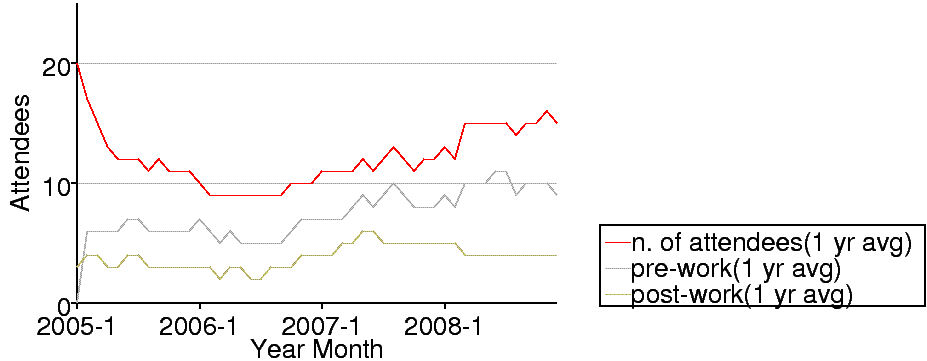
\includegraphics[width=1\hsize]{image200812/memberanalysis/attend.png}
\caption{$BEl5~%(%j%"(BDebian$BJY6/2q;vA02]Bj!&;v8e2]BjDs=P<B@S(B(12$B%v7n0\F0J?6Q(B)}\label{fig:attendandprepostwork}
\end{figure}

\begin{table}[ht]
 \caption{$BEl5~%(%j%"(BDebian$BJY6/2q;vA02]Bj!&;v8e2]BjDs=P<B@S(B}\label{tab:attendandprepostwork}
\begin{minipage}{0.5\hsize}
\begin{tabular}{|l|r|r|r|r|}
 \hline
   $BG/(B&$B7n(B & $B;22C?M?t(B & $B;vA02]Bj!!(B& $B;v8e2]Bj(B \\
 \hline
 2005 & 1 & 20 & 0 & 3 \\
 2005 & 2 & 15 & 12 & 6 \\
 2005 & 3 & 10 & 8 & 4 \\
 2005 & 4 & 9 & 6 & 2 \\
 2005 & 5 & 6 & 6 & 4\\
 2005 & 6 & 13 & 10 & 5\\
 2005 & 7 & 12 & 7 & 4\\
 2005 & 8 & 9 & 6 & 2\\
 2005 & 9 & 14 & 7 & 4\\
 2005 & 10 & 10 & 5 & 3\\
 2005 & 11 & 7 & 6 & 3\\
 2005 & 12 & 8 & 5 & 3\\
 2006 & 1 & 9 & 7 & 3\\
 2006 & 2 & 8 & 4 & 2\\
 2006 & 3 & 6 & 0 & 0\\
 2006 & 4 & 15 & 11 & 6\\
 2006 & 5 & 7 & 2 & 1\\
 2006 & 6 & 14 & 9 & 4\\
 2006 & 7 & 2 & 2 & 4\\
 2006 & 8 & 17 & 9 & 7\\
 2006 & 9 & 12 & 8 & 5\\
 2006 & 10 & 22 & 15 & 7\\
 2006 & 11 & 3 & 12 & 7\\
 2006 & 12 & 15 & 7 & 4\\
\end{tabular}
\end{minipage}
\begin{minipage}{0.5\hsize}
\begin{tabular}{|l|r|r|r|r|}
 \hline
   $BG/(B&$B7n(B & $B;22C?M?t(B & $B;vA02]Bj!!(B& $B;v8e2]Bj(B \\
 \hline
 2007 & 1 & 15 & 6 & 4\\
 2007 & 2 & 13 & 8 & 4\\
 2007 & 3 & 0 & 6 & 16\\
 2007 & 4 & 18 & 14 & 6\\
 2007 & 5 & 21 & 14 & 7\\
 2007 & 6 & 1 & 0 & 1\\
 2007 & 7 & 18 & 12 & 3\\
 2007 & 8 & 25 & 18 & 5\\
 2007 & 9 & 0 & 7 & 5\\
 2007 & 10 & 10 & 1 & 6\\
 2007 & 11 & 19 & 10 & 6\\
 2007 & 12 & 11 & 11 & 4\\
 2008 & 1 & 22 & 11 & 4\\
 2008 & 2 & 0 & 1 & 0\\
 2008 & 3 & 37 & 27 & 11\\
 2008 & 4 & 17 & 13 & 3\\
 2008 & 5 & 20 & 14 & 3\\
 2008 & 6 & 10 & 8 & 2\\
 2008 & 7 & 17 & 12 & 4\\
 2008 & 8 & 10 & 0 & 4\\
 2008 & 9 & 17 & 13 & 5\\
 2008 & 10 & 11 & 0 & 7\\
 2008 & 11 & 22 & 14 & 6\\
\end{tabular}
\end{minipage}

\end{table}

$B:rG/$+$i$OJY6/2q$OEl5~$H4X@>$NN>J}$G3+:E$5$l$k$h$&$K$J$C$F$$$^$9!#(B
$BEl5~%(%j%"(BDebian$BJY6/2q$H!"4X@>(BDebian$BJY6/2q$K$D$$$F4JC1$K=P@J?t$G<B@S$r$_$F$_$^$7$g$&!#(B
$B$^$:!"El5~$K$D$$$F%0%i%U$K$7$F$_$k$H(B\fgref{fig:peoplechart-1}$B$K$J$j$^$9!#(B

\begin{figure}[h]
 \begin{center}
  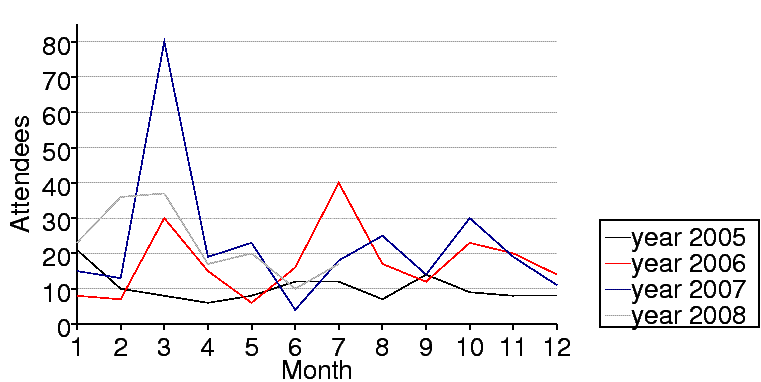
\includegraphics[width=1\hsize]{image200812/people-chart.png}
  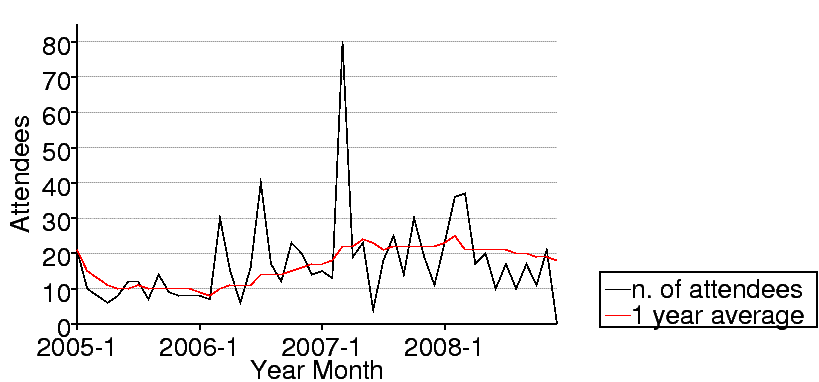
\includegraphics[width=1\hsize]{image200812/serialized.png}
 \end{center}
\caption{$BEl5~%(%j%"(BDebian$BJY6/2q$N;22C?M?t?d0\(B}
\label{fig:peoplechart-1}
\end{figure}


$B6qBNE*$J?t;z$H!"%H%T%C%/$r8+$F$_$^$7$g$&!#(B
 
\begin{table}[ht]
\begin{minipage}{0.5\hsize}
 \caption{$BEl5~%(%j%"(BDebian$BJY6/2q;22C?M?t(B(2005$BG/(B)}\label{tab:count-1}
 \begin{center}
  \begin{tabular}{|l|c|p{10em}|}
 \hline
   & $B?M?t(B & $BFbMF(B \\
 \hline
   2005$BG/(B1$B7n(B & 21 & $BHkL)(B\\
   2005$BG/(B2$B7n(B & 10 & debhelper1\\
   2005$BG/(B3$B7n(B & 8 &  ($BAaD+(B) debhelper2$B!"(Bsocial contract\\
   2005$BG/(B4$B7n(B & 6 & debhelper3\\
   2005$BG/(B5$B7n(B & 8 & DFSG$B!"(Bdpkg-cross$B!"(Blintian/linda\\
   2005$BG/(B6$B7n(B & 12 & alternatives$B!"(Bd-i\\
   2005$BG/(B7$B7n(B & 12 & toolchain$B!"(Bdpatch\\
   2005$BG/(B8$B7n(B & 7 & Debconf$B;22CJs9p!"(BITP$B$+$i%"%C%W%m!<%I$^$G(B\\
   2005$BG/(B9$B7n(B & 14 & debconf\\
   2005$BG/(B10$B7n(B & 9 & apt-listbugs$B!"%P%0%l%]!<%H!"(Bdebconf$BK]Lu!"(Bdebbugs\\
   2005$BG/(B11$B7n(B & 8 & DWN$BK]Lu%U%m!<!"(Bstatoverride\\
   2005$BG/(B12$B7n(B & 8 & $BK:G/2q(B\\
 \hline
  \end{tabular}
 \end{center}
\end{minipage}
\begin{minipage}{0.5\hsize}
 \caption{$BEl5~%(%j%"(BDebian$BJY6/2q;22C?M?t(B(2006$BG/(B)}\label{tab:count2006-1}
 \begin{center}
  \begin{tabular}{|l|c|p{10em}|}
 \hline
 & $B;22C?M?t(B & $BFbMF(B\\
 \hline
 2006$BG/(B1$B7n(B & 8 & policy$B!"(BDebian$BJY6/2q$G$d$j$?$$$3$H(B\\
 2006$BG/(B2$B7n(B & 7 & policy$B!"(Bmultimedia \\
 2006$BG/(B3$B7n(B & 30 & OSC: debian$BJY6/2q!"(Bsid \\
 2006$BG/(B4$B7n(B & 15 & policy$B!"(B\LaTeX{} \\
 2006$BG/(B5$B7n(B & 6 & mexico \\
 2006$BG/(B6$B7n(B & 16 & debconf$B!"(Bcowdancer\\
 2006$BG/(B7$B7n(B & 40 & OSC-Do: MacBook Debian \\
 2006$BG/(B8$B7n(B & 17 & 13$B<9G0(B \\
 2006$BG/(B9$B7n(B & 12 & $BK]Lu!"(BDebian-specific$B!"(Boprofile \\
 2006$BG/(B10$B7n(B & 23 & network$B!"(Bi18n$B2q5D!"(BFlash$B!"(Bapt \\
 2006$BG/(B11$B7n(B & 20 & $B4X@>3+:E!'(B bug$B!"(Bsid$B!"(Bpackaging \\
 2006$BG/(B12$B7n(B & 14 & $BK:G/2q(B \\
 \hline
  \end{tabular}
 \end{center}
\end{minipage}
 \end{table}

\begin{table}[t]
\begin{minipage}{0.5\hsize}
 \caption{$BEl5~%(%j%"(BDebian$BJY6/2q;22C?M?t(B(2007$BG/(B)}\label{tab:count2007-1}
 \begin{center}
  \begin{tabular}{|l|c|p{10em}|}
 \hline
 & $B;22C?M?t(B & $BFbMF(B\\
 \hline
2007$BG/(B1$B7n(B & 15 & $B0lG/$r4k2h$9$k(B \\
2007$BG/(B2$B7n(B & 13 & dbs, dpatch\\ 
2007$BG/(B3$B7n(B & 80 & OSC$B2>A[2=(B \\
2007$BG/(B4$B7n(B & 19 & quilt, darcs, git\\
2007$BG/(B5$B7n(B & 23 & etch, pbuilder, superh \\   
2007$BG/(B6$B7n(B & 4 & $B%(%8%s%P%i3+:E!'(BDebconf7 $B<B67Cf7Q(B \\
2007$BG/(B7$B7n(B & 18 & Debconf7 $B;22CJs9p(B\\
2007$BG/(B8$B7n(B & 25 & cdn.debian.or.jp \\   
2007$BG/(B9$B7n(B & 14 & exim \\   
2007$BG/(B10$B7n(B & 30 & OSC Tokyo/Fall(CUPS) \\   
2007$BG/(B11$B7n(B & 19 & live-helper, tomoyo linux kernel patch, server\\
2007$BG/(B12$B7n(B & 11 & $BK:G/2q(B\\
 \hline
  \end{tabular}
 \end{center}
\end{minipage}
\begin{minipage}{0.5\hsize}
 \caption{$BEl5~%(%j%"(BDebian$BJY6/2q;22C?M?t(B(2008$BG/(B)}\label{tab:count2008-1}
 \begin{center}
  \begin{tabular}{|l|c|p{10em}|}
 \hline
 & $B;22C?M?t(B & $BFbMF(B\\
 \hline
2008$BG/(B1$B7n(B & 23 & $B0lG/$r4k2h$9$k(B \\
2008$BG/(B2$B7n(B29+1$BF|(B & 36 & OSC  \\
2008$BG/(B3$B7n(B & 37 & $B%G!<%?$@$1$N%Q%C%1!<%8!"%i%$%;%s%9(B \\
2008$BG/(B4$B7n(B & 17 & $B%P%$%J%j%Q%C%1!<%8(B \\
2008$BG/(B5$B7n(B & 20 & $BJ#?t$N%P%$%J%j%Q%C%1!<%8(B \\
2008$BG/(B6$B7n(B & 10 & debhelper \\
2008$BG/(B7$B7n(B & 17 & Linux kernel patch / module $B%Q%C%1!<%8(B \\
2008$BG/(B8$B7n(B & 10 & Debconf IRC$B2q5D$H(BDebian$B29@t(B \\
2008$BG/(B9$B7n(B & 17 & po4a, $B!V(BDebian $B%a%s%F%J$N$*;E;v!W(B \\
2008$BG/(B10$B7n(B & 11? & OSC Tokyo/Fall \\
2008$BG/(B11$B7n(B & 17 & $B!V$=$N>l$GJY6/2q;qNA$r:n@.$7$A$c$(!W(B Debian $B$r;H$C$?(B \LaTeX{} $B869F:n@.9g=I(B \\
2008$BG/(B12$B7n(B & ? & $BK:G/2q(B \\
 \hline
  \end{tabular}
 \end{center}
\end{minipage}
\end{table}

$B$=$l$G$O!"4X@>(BDebian$BJY6/2q$N=P@J>u67$r3NG'$7$F$_$^$7$g$&!#(B
$B%0%i%U$G8+$k$H(B\fgref{fig:kansaipeoplechart-1}$B$K$J$j$^$9!#(B
$BI=$G8+$k$H(B\tbref{tab:count2007kansai-1}$B$K$J$j$^$9!#(B

\begin{figure}[h]
 \begin{center}
  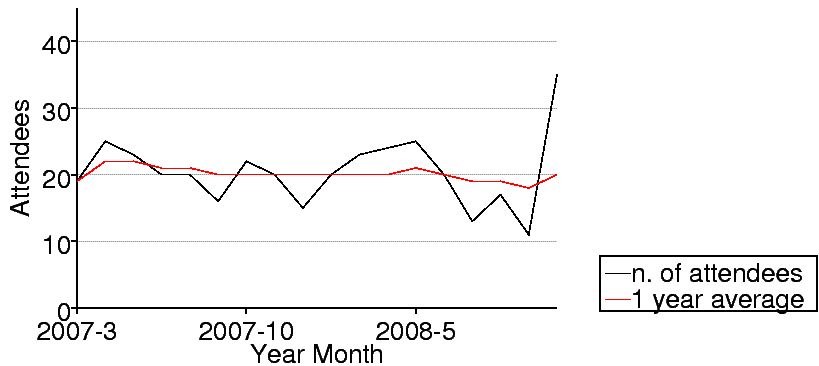
\includegraphics[width=1\hsize]{image200812/kansai.png}
 \end{center}
\caption{$B4X@>$N;22C?M?t?d0\(B}
\label{fig:kansaipeoplechart-1}
\end{figure}


\begin{table}
\begin{minipage}{0.5\hsize}
 \caption{$B4X@>(BDebian$BJY6/2q;22C?M?t(B(2007$BG/(B)}\label{tab:count2007kansai-1}
 \begin{center}
  \begin{tabular}{|l|c|p{10em}|}
 \hline
 & $B;22C?M?t(B & $BFbMF(B \\
 \hline
2007$BG/(B3$B7n(B & 19 & $B3+:E$K$"$?$j(B \\
2007$BG/(B4$B7n(B & 25 & goodbye$B!"(Byoutube$B!"%W%m%8%'%/%H%H%i%C%+!<(B\\
2007$BG/(B6$B7n(B & 23 & $B<R2q7@Ls!"%F!<%^!"(Bdebian/rules$B!"(Bbugreport\\
2007$BG/(B7$B7n(B & 20$BA08e(B & OSC-Kansai \\
2007$BG/(B8$B7n(B & 20 & Inkscape$B!"(Bpatch$B!"(Bdpatch\\
2007$BG/(B9$B7n(B & 16 & $B%i%$%V%i%j!"K]Lu!"(Bdebtorrent\\
2007$BG/(B10$B7n(B & 22& $BF|K\8lF~NO!"(BSPAM$B%U%#%k%?(B\\
2007$BG/(B11$B7n(B & 20$BA08e(B & KOF \\   
2007$BG/(B12$B7n(B & 15& $BK:G/2q!"(BiPod touch\\   
 \hline
  \end{tabular}
 \end{center}
\end{minipage}
\begin{minipage}{0.5\hsize}
 \caption{$B4X@>(BDebian$BJY6/2q;22C?M?t(B(2008$BG/(B)}\label{tab:count2008kansai-1}
 \begin{center}
  \begin{tabular}{|l|c|p{10em}|}
 \hline
 & $B;22C?M?t(B & $BFbMF(B \\
 \hline
2008$BG/(B2$B7n(B & 20 & PC Cluster, GIS, \TeX \\
2008$BG/(B3$B7n(B & 23 & bug report, developer corner, GPG \\
2008$BG/(B4$B7n(B & 24 & coLinux, Debian GNU/kFreeBSD, sid \\
2008$BG/(B5$B7n(B & 25  & ipv6, emacs, ustream.tv\\
2008$BG/(B6$B7n(B & 20  & pbuilder, hotplug, ssl\\
2008$BG/(B8$B7n(B & 13  & coLinux \\
2008$BG/(B9$B7n(B & 17  & debian mentors, ubiquity, DFSG\\
2008$BG/(B10$B7n(B & 11  & cdbs,cdn.debian.or.jp \\
2008$BG/(B11$B7n(B & 35  & KOF \\
2008$BG/(B12$B7n(B & ?  & \\
 \hline
  \end{tabular}
 \end{center}
\end{minipage}
\end{table}

\clearpage

\dancersection{2008$BG/$r?6$jJV$C$F$_$k(B}{$B>e@n(B $B=c0l(B}

\subsection{$B:G6a$N%H%l%s%I$H:#8e$N?d0\(B}

$B:G6a$I$s$J$3$H$,(B
$B$"$C$F!"$3$l$+$i$I$&$$$&$3$H$,$"$k$G$7$g$&$+!#(B
$B$_$s$J$GM=A[$7$F$_$^$7$g$&!#(B

{\footnotesize
\begin{tabular}[t]{|p{8em}|p{8em}|p{12em}|p{8em}|p{8em}|}
\hline
2006 &2007 &2008 &2009 & 2010 \\
\hline
%2006
IntelMac$B$K!"(Bcoreduo$B$G(Bdual-core CPU $B$K!"(B 

glantank(ARM)$B!"(B 
OpenMicroServer(MIPS)$B!"(B 

OpenSolaris$B$,=P$F(BDebian/Solaris (Nexenta) $BEP>l!"(B 
SparcT1$B$,%*!<%W%s$K!"(B

CC3.0$B!"(B

Qwik$BEP>l(B(?)$B!"(B

$B;(;o$,BgB??t>C<:!"(B

 &
%2007
VT$B!&(BAMD-V($B2>A[2=5;=Q(B)$B$,Ia5Z(B(ML115!)$B!"(B

$B9uH"(B(ARM)$B!"(B
OpenBlocks(PPC?)$B!"(B
iPhone$BEP>l!"(B 
HSDPA $B7n3[(B5000$B1_$/$i$$$K!"(B
google mobile$B!"(B

VISTA$B%j%j!<%9!"(B 
Leopard$B%j%j!<%9!"(B 

GPL3.0$B!"(B
$B%a%b%j(B2G$B$,%3%b%G%#%F%#!<$K!"(B
SparcT2$B$,%*!<%W%s!"(B 
$B%K%3%K%3F02h!"(B
& 
%2008
python 3.0
ruby 1.9

wine 1.0, wine64 $BEP>l(B

RoR 2.0 $BEP>l$GIa5Z$K(B

4$B%3%"!&(B64bit $B$N(BCPU$B$,%G%9%/%H%C%W$KIa5Z!"(B
Core2Quad $BCM2<$2!#(B

$B%K%3%K%3F02h(B1000$BK|%f!<%6FMGK!"(B
$B=i2;%_%/%V!<%`$K(B

$BCO%G%84XO"$N(BPC$B@=IJ$NIa5Z(B

$BJY6/2q$NIa5Z(B($B3ZE7$H$+(B)

$B8x=0L5@~(BLAN (wireless gate)

$B7HBSEEOC$NGd>e$,Mn$A$k!"(B
iPhone, Android $BEP>l!"(B
emobile 100$B1_(BPC$BJz$-$"$o$;(B
(eeePC, Dell mini9)
Zaurus$BHNGd=*N;!#(B

Chumby $BH/Gd!#(B

$B%5!<%P$N2>A[2=(B ESXi$B!&%7%s%/%i%$%"%s%H(B

MacBook Air $BH/Gd!"(B
$BL5@~(B 802.11n $B$,<B5!$K(B

SystemZ10 $BH/I=(B

$B@$3&7P:Q$NJx2u(B(IT$BEj;q6[=L:b@/!"?&$r<:$&?M$,A}2C(B)

FreeBSD 7 (malloc, ZFS ?)

Debian$B<!@$Be0i@.7W2h;OF0(B

Debian Maintainer $B@)EY;OF0(B

$B%;%-%e%j%F%#!<4XO"(B(OpenSSL $B;v7o!"(BDNS$B;v7o(B)

$B%/%i%&%I4XO"$,N.9T(B?

Nintendo DSi

&
%2009

tile window manager boom ?

Lenny $B%j%j!<%9M=Dj(B

Debian $B9gF17k:'<0(B

$B%G%9%/%H%C%W!"(B8$B%3%"!"(B4GB? 8GB?

$B%N!<%H%Q%=%3%s!"(B2$B%3%"!"(B2GB?

Linux $B$,I8=`%$%s%9%H!<%k$N(BPC$B!#(B

SSD $B$NCMCJ$HMFNL$,$3$J$l$k(B?
HDD$B$,$J$/$J$k(B?$B9b$/$J$k(B?

$B%U%!%$%k%7%9%F%`$+$o$k(B?

ipv6 $B;H$($k$h$&$K$J$C$F$k(B?

Bluray $B$,Ia5Z(B?

DL$B6X;_K!(B? torrent $B$K5UIw(B?

&
%2010

$B>CHq@G>e>:$KH<$&HKK;4|(B

$B%/%i%&%I$K$h$j!"C1=c$J%[%9%F%#%s%06H<T$,$D$E$+$J$$(B?
$B0lIt$O<+<R$G$b$D$h$&$K$J$k(B?

Squeeze$B%j%j!<%9(B

USB 3.0 $BEk:\!"(Bwireless USB vs Bluetooth ?

$BAH$_9~$_(BCPU$B$O(BAtom$B$KE}0l(B?Arm$B$O;D$C$F$k(B?

kFreeBSD $B%*%U%#%7%c%k%"!<%-%F%/%A%c$K(B

ruby 2.0 $B%j%j!<%9(B?

 \\

\hline
\end{tabular}

}

\subsection{SWOT}

%SWOT
{\large
\begin{tabular}[t]{|p{8em}|p{8em}|p{8em}|p{8em}|}
\hline
$B$G$-$?$3$H(B & $B$G$-$J$+$C$?$3$H(B & $B%A%c%s%9$H$J$k$b$N(B & $B6<(B
 $B0R$H$J$k$b$N(B \\
\hline
%S 
$B2G$,$G$-$?!#(B(20\%$B!"(B10\% 2$B<!85(B)
$B>-Mh$N(BDD$B$,@8$^$l$?!#(B

Hands-on($B%Q%C%1!<%8:n@.$H(B\LaTeX{}) $B$H9g=I(B($B29@t$H%V%l%9%H(B)$B!"(B
DMC$B$,$G$-$?!#(B

$B;}$A2s$j$GH/I=$9$k(B

$B>l=j$,$$$m$$$m$@$C$?!#(B($B>e@nIT:_(B)

$BB>$NJY6/2q(B($B%+!<%M%kFI=q2q(B)$B$K2%$j9~$_(B($B4d>>!";3:,(B)

Ubuntu$B$H$N8rN.!"(BDebian JP$B$K4sIU(B



&
%W

$BEv=i$NL\I8$G$"$C$?=w;R9b@8!"Bg3X@8$X$N4+M6$,@.8y$7$J$+$C$?!#(B

$B2G$,$G$-$J$+$C$?(B(70\%$B!"A[A|NO$,$?$j$J$$(B)

$BH/I=$d$j$?$+$C$?$1$I$G$-$J$+$C$?(B($B$G$s$5$s(B)

GNU/Hurd$B!"(BSuperH

Debconf$B$K$$$1$J$+$C$?(B($B>e@n0J30(B)

$BF|K\$X$N(BDebconf$B>7CW3hF0L$40(B

&
%O
	 
$B=jBS;}$A%O%C%/J}K!$,@8$^$l$k(B($B$$$+$K$7$F;~4V$r$D$/$k$+(B)$B!#(B

$BL5BL$JGc$$J*$r$7$J$/$J$k!#(B
$B%O%C%/$7$J$$$H!#(B

$BEl5~%*%j%s%T%C%/$N@.N)(B?

$B3X@8$N="?&N(Dc2<!"Bg3X1!@8A}2C(B?$B%K!<%HA}2C(B?

GPLv3 $B$NIa5Z(B?
Android?

&
%T

$B4D6-@0Hw$,$G$-$J$/$J$k(B(
$B%\!<%J%9$,8:$C$?!"(B
$B;E;v$,$J$/$J$k$+$b(B)

Atom $B$K$h$k(BCPU$B%"!<%-%F%/%A%c!<$N6nC`(B

$B%O%C%/$G$-$J$$%G%P%$%9$NA}2C(B($BEEOC$H$+(B)

$BK!@)EY$N6/2=$K$h$j<+M3$,$&$P$o$l$k(B?

$B=>NL@)2]6b$K0\9T(B?

\\
\hline
\end{tabular}
}

\clearpage

\subsection{SWOT 2}

% SWOT 2
\begin{tabular}[t]{|p{4em}|p{11em}|p{11em}|p{11em}|}
\hline
 &  & $B%A%c%s%9$H$J$k$b$N(B & $B6<0R$H$J$k$b$N(B  \\\hline
\vspace{0.2\vsize}~

 & & 
%O
	 
$B=jBS;}$A%O%C%/J}K!$,@8$^$l$k(B($B$$$+$K$7$F;~4V$r$D$/$k$+(B)$B!#(B

$BL5BL$JGc$$J*$r$7$J$/$J$k!#(B
$B%O%C%/$7$J$$$H!#(B

$BEl5~%*%j%s%T%C%/$N@.N)(B?

$B3X@8$N="?&N(Dc2<!"Bg3X1!@8A}2C(B?$B%K!<%HA}2C(B?

GPLv3 $B$NIa5Z(B?
Android?

&
%T

$B4D6-@0Hw$,$G$-$J$/$J$k(B(
$B%\!<%J%9$,8:$C$?!"(B
$B;E;v$,$J$/$J$k$+$b(B)

Atom $B$K$h$k(BCPU$B%"!<%-%F%/%A%c!<$N6nC`(B

$B%O%C%/$G$-$J$$%G%P%$%9$NA}2C(B($BEEOC$H$+(B)

$BK!@)EY$N6/2=$K$h$j<+M3$,$&$P$o$l$k(B?

$B=>NL@)2]6b$K0\9T(B?

\\
\hline
$B$G$-$?$3$H(B & 
%S

$B2G$,$G$-$?!#(B(20\%$B!"(B10\% 2$B<!85(B)
$B>-Mh$N(BDD$B$,@8$^$l$?!#(B

Hands-on($B%Q%C%1!<%8:n@.$H(B\LaTeX{}) $B$H9g=I(B($B29@t$H%V%l%9%H(B)$B!"(B
DMC$B$,$G$-$?!#(B

$B;}$A2s$j$GH/I=$9$k(B

$B>l=j$,$$$m$$$m$@$C$?!#(B($B>e@nIT:_(B)

$BB>$NJY6/2q(B($B%+!<%M%kFI=q2q(B)$B$K2%$j9~$_(B($B4d>>!";3:,(B)

Ubuntu$B$H$N8rN.!"(BDebian JP$B$K4sIU(B

&

$BEl5~%*%j%s%T%C%/$N2q>l$G%O%C%/!#(B

$B3X9;$K$*4j$$$7$F3X@8$r4+M6$9$k!&%O%s%:%*%s!#(B

$B!V7/$N$5$o$C$F$$$k(BXX$B$O(BLinux$B$@$1$I$h$j>\$7$/CN$j$^$;$s$+(B?$B!W(B
($B%_%K%N!<%H$N%W%j%$%s%9%H!<%k!"7HBS!"(BAndroid)

& 

$B$h$j$h$$%M%C%H%o!<%/%W%m%H%3%k$r<B;\(B

$B%"%s%A(BAtom?

\\
\hline

$B$G$-$J$+$C$?$3$H(B
&
%W

$BEv=i$NL\I8$G$"$C$?=w;R9b@8!"Bg3X@8$X$N4+M6$,@.8y$7$J$+$C$?!#(B

$B2G$,$G$-$J$+$C$?(B(70\%$B!"A[A|NO$,$?$j$J$$(B)

$BH/I=$d$j$?$+$C$?$1$I$G$-$J$+$C$?(B($B$G$s$5$s(B)

GNU/Hurd$B!"(BSuperH

Debconf$B$K$$$1$J$+$C$?(B($B>e@n0J30(B)

$BF|K\$X$N(BDebconf$B>7CW3hF0L$40(B

&

Debconf $B$K$$$/!#(B

$B;~4V$r$D$/$k!"%i%$%U%O%C%/(B($B=jBS;}$A%O%C%/(B)$B!#(B

$B@lLg3X9;!"9)6H9b9;!"Bg3X$G$N3+:E!#(B


$B8@8l7O$N%3%_%e%K%F%#!<$K@Z$j9~$`(B

$B%$%s%U%i7O$N?M$?$A$K@Z$j9~$`(B

$BHs>o6P9V;U$K$J$k!#(B

&

\\
\hline
\end{tabular}

\dancersection{sqlite3 $B$H(B python $B$G(B csv $B%U%!%$%k$rJ,@O$9$k(B}{$B>e@n=c0l(B}
\label{sqlite3intro}
\index{sqlite}

sqlite $B$O$*<j7Z$K(B SQL $B$rMxMQ$9$k$?$a$N;EAH$_$G$9!#%G!<%?%Y!<%9$,0l$D$N(B
UNIX$B%U%!%$%k$H$7$F4IM}$5$l$F$*$j!"%G!<%?%Y!<%9$N:n@.!&:o=|$,4JJX$K9T$&$3(B
$B$H$,$G$-$k$3$H!"$^$?!"%5!<%P%/%i%$%"%s%H%"!<%-%F%/%A%c$G$O$J$/!"(BOS$B$NDs6!(B
$B$9$k%U%!%$%k%7%9%F%`$N%m%C%/5!9=$r3hMQ$7$F(BACID$BFC@-$r<B8=$7$F$$$k$H$$$&FC(B
$BD'$,$"$j$^$9(B
(\fgref{fig:sqlitestructure})\footnote{\url{http://www.sqlite.org/atomiccommit.html}
$B$K;EAH$_$N@bL@$,$"$j$^$9(B}$B!#(B
$B%G!<%?%Y!<%9$rMxMQ$9$k>l9g$K$*$$$F$O!"%G!<%?%Y!<%9$r%5!<%P%/%i%$%"%s%H%b%G%k$GMxMQ$7$h$&(B
$B$H$9$k$H!"(B
$B%G!<%?%Y!<%9%U%!%$%kCV$->l$d%]!<%HHV9f$d%[%9%HL>$d(B
$B%f!<%6L>$d%Q%9%o!<%I$N@_Dj$,:GDc$G$bI,MW$K$J$j$^$9$,!"$=$l$i$,I,MW$J$/$J(B
$B$j$^$9!#(B
$B$=$N$?$a!"%G!<%?%Y!<%9$N%$%s%9%?%s%9$rJL$KN)$A>e$2$J$/$F$b$h$$$s$@$1$I!"(B
$B$A$g$C$H(B SQL $B$r;H$$$?$$$H$$$&$h$&$J%/%$%C%/%O%C%/$KJXMx$G$9!#(B

\begin{figure}[ht]
\begin{center}
 \fbox{\includegraphics[width=0.5\hsize]{image200812/sqlite.eps}}
\end{center}
\caption{$B0lHLE*$J(BDB$B$H(B sqlite$B$N0c$$(B}\label{fig:sqlitestructure}
\end{figure}

$B$^$:!"$3$N5-;v$KI,MW$J4XO"%Q%C%1!<%8$r%$%s%9%H!<%k$7$^$7$g$&!#(B

\begin{commandline}
$ sudo apt-get install sqlite3 python-pysqlite2
\end{commandline}

\subsection{$B%G!<%?%Y!<%9$N:n@.(B}

sqlite3$B$H$$$&(BCUI$B$N%"%W%j%1!<%7%g%s$,$"$j!"0lHLE*$J(B SQL $BJ8$rMxMQ$9$k$3$H$,(B
$B$G$-$^$9!#$^$?!"(Bruby, perl, ocaml, haskell, common lisp, Smalltalk $B$J$I$N(B
$B0lHLE*$J%W%m%0%i%_%s%08@8lMQ$N%P%$%s%G%#%s%0$bMQ0U$5$l$F$*$j!"%G!<%?%Y!<(B
$B%9$rMxMQ$9$k$3$H$,$G$-$^$9!#(B

$B$^$:!"%G!<%?%Y!<%9$r:n@.$7$F$_$^$7$g$&!#(B

\begin{commandline}
$ sqlite3 debmtg.db
sqlite> 
\end{commandline}

$BB8:_$7$J$$?7$7$$%U%!%$%kL>$r;XDj$9$l$P!"$=$N%U%!%$%kL>$G%G!<%?%Y!<%9$,:n@.$5$l$^$9!#(B
$B$3$N;~E@$G(BSQL$BJ8(B(CREATE TABLE)$B$J$I$,MxMQ$G$-$^$9!#(B

\subsection{$B%G!<%?$r$D$C$3$`(B}

$B%G!<%?%Y!<%9$b:n@.$G$-$?$N$G!"%G!<%?$r$D$C$3$s$G$_$^$7$g$&!#(B
csv $B%U%!%$%k$+$i%G!<%?%Y!<%9$K%G!<%?$rA^F~$9$k%1!<%9$r9M$($F$_$^$9!#(B
$B<B$O(Bsqlite3 $B$N(B \texttt{.import} $B%3%^%s%I$r;H$($P$h$$$N$G$9$,!"$3$3$G$O(B
$B%W%m%0%i%`8@8l$N%P%$%s%G%#%s%0$r3hMQ$7$F%$%s%]!<%H$7$F$_$^$9!#(B

$B$^$:!"(Bcsv$B7A<0$G%G!<%?$rMQ0U$7$^$9!#(B
\begin{commandline}
$B>e@n(B,10
$B4d>>(B,15
$B;3ED(B,9
\end{commandline}

csv $B%U%!%$%k$rFI$_9~$_(B SQL $B%3%^%s%I$r=PNO$9$k(B python $B$N%3!<%I$r=q$-$^$9!#(B

\commandlineinput{image200812/test.py}

\subsection{SQL$B$r;H$C$F$_$k(B}

sqlite3 $B%3%^%s%I$r<B9T$9$k$H%$%s%?%i%/%F%#%V$K(BSQL$BJ8$rF~NO$9$k$3$H$,2DG=(B
$B$G$9!#(B

$B$^$:!"(Bsqlite $BFH<+$NL?Na$r$D$+$C$F%G!<%?%Y!<%9$N9=B$$rJ,@O$7$F$_$^$9!#(B

\begin{commandline}
$ sqlite3 debmtg.db
sqlite> .tables
test
sqlite> .dump test
BEGIN TRANSACTION;
CREATE TABLE test(name text, score number);
INSERT INTO "test" VALUES('$B>e@n(B',10);
INSERT INTO "test" VALUES('$B4d>>(B',15);
INSERT INTO "test" VALUES('$B;3ED(B',9);
COMMIT;
\end{commandline}

SQL $BJ8$G%i%s%-%s%0$rD4$Y$?$jJ?6QCM$rD4$Y$?$j$b$G$-$^$9!#(B

\begin{commandline}
sqlite> select name, score from test order by score; 
$B;3ED(B|9
$B>e@n(B|10
$B4d>>(B|15
sqlite> select sum(score)/count(score) from test; 
11
\end{commandline}

$B0J>e!"4JC1$G$9$,!"(B sqlite $B$N>R2p$G$7$?!#(B

% from debianmeetingresume200901.tex
\dancersection{Debian JP $BDjNc2q5D(B on IAX}{$B>e@n=c0l(B}
%\subsection{Debian JP $BDjNc2q5D(B on IAX}

Debian JP $B$NDjNc2q5D$ODL>o(B IRC $B$G9T$C$F$$$k$N$G$9$,!"(B2009$BG/(B1$B7n(B8$BF|$K<9$j9T(B
$B$o$l$?2q5D$O<B83E*$K2;@<DLOC$b8r$($F9T$$$^$7$?!#MxMQ$7$?%W%m%H%3%k$O(BIAX$B%W(B
$B%m%H%3%k$G!"(Biaxcomm $B$r%/%i%$%"%s%H$H$7$FMxMQ$7!"(Basterisk $B%5!<%P$KA40w@\B3(B
$B$7$^$7$?!#(B

MacBook$B$N%^%$%/$^$o$j$N%O%C%/$,==J,$G$J$/!"(Biaxcomm $B<+BN$N0BDjEY9g$$$b$h$/(B
$B$J$+$C$?$N$G2;<A$,0-$$$H$$$&LdBj$,$"$j$^$7$?$,DL?.>uBV$O35$MNI9%$G$7$?!#(B
$B:#8e$5$i$K;n83$r=E$M$F<BMQE*$K;H$C$F9T$-$?$$$b$N$G$9!#(B


% ===============================================================
\dancersection{Git+$B%a!<%k$G$N;vA02]BjDs=P$K$^$D$o$k2]Bj(B}{$B>e@n=c0l(B}
\index{git}
% ===============================================================

2008$BG/(B11$B7n!"(B12$B7n!"$*$h$S(B2009$BG/(B1$B7n$K$O;vA02]Bj$r(BGit$B$rMxMQ$7$F(BGit$B$N@8@.$9$k(B
$B%Q%C%A$r%a!<%k$GDs=P$7$F$b$i$&$H$$$&7A<0$K$7$F$$$^$7$?!#(B
$B$=$N>l9g$K$O(B git pull $B$9$k$?$S$K%3%s%U%j%/%H$,H/@8$7$^$9!#(B
$B$=$N860x$H$J$k;EAH$_$HBP:vJ}K!$K$D$$$F@bL@$7$^$9!#(B

\subsection{$B%3%s%U%j%/%H$,H/@8$7$d$9$$M}M3(B}

$B$=$l$G$O!"(BDebian $BJY6/2q$N(B2008$BG/(B11,12$B7n$N;qNA$G%3%s%U%j%/%H$,H/@8$7$d$9$+$C(B
$B$?M}M3$rJ,@O$7$F$_$^$7$g$&!#(B

\subsubsection{$B85$N%U%!%$%k$N7A<0(B}

\begin{commandline}
-\subsection{}
+\subsection{XXXX}
+$BFbMF(B
+
\end{commandline}

$BF1$8%U%!%$%k$K$D$$$F:n6H$7!"$7$+$bF1$8>l=j$K$9$3$7$E$D0[$J$kJQ99$rJL$N?M(B
$B$,9T$&$H$$$&;EAH$_$K$J$C$F$$$^$7$?!#$3$N>l9g!"Fs$D$N%Q%C%A$O$+$J$i$:%3%s(B
$B%U%j%/%H$7!"<jF0$G2r>C$9$kI,MW$,$"$j$^$9!#:#2s%Q%C%A$,F1$8>l=j$KA^F~$7$F(B
$B$$$k>l9g$K!"=g=x$OLd$o$J$$$N$GE,Ev$G$h$$$N$G$9$,!"(B\texttt{git apply} $B$K$O(B
$B$=$NCN<1$O$J$$$?$a!"Kh2s%3%s%U%j%/%H$N2r>C$r9T$$$^$9!#(B

\subsubsection{$B%a!<%k$rMxMQ$7$?%5%V%_%C%H(B}

\begin{figure}
 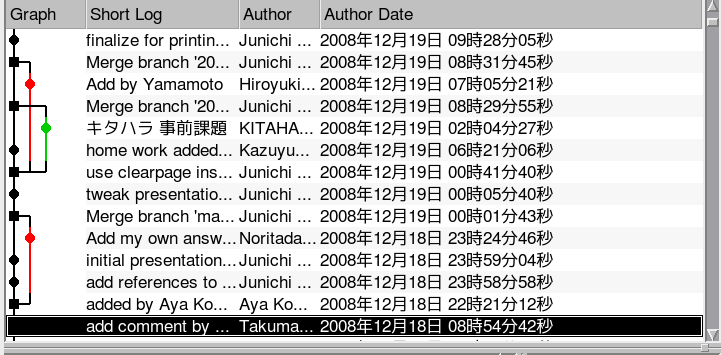
\includegraphics[width=\hsize]{image200901/qgit-trees.png}
 \caption{qgit$B$G$_$?%D%j!<$N>u67!"<jF0$G%^!<%8$,J#?tH/@8$7$F$$$k(B}
 \label{fig:mergedtokyodebian}
\end{figure}

$BDy@Z$jD>A0$K:n6H$9$k$N$,=,47$N$?$a!"(B
$BJ#?t$N?M$,$"$k;~E@$NF1$8%3%_%C%H$KBP$7$F%Q%C%A$r:n@.!"(B
$B$=$l$r>e@n$,$"$k;~E@$G%^!<%8$7$^$7$?(B(\fgref{fig:mergedtokyodebian})$B!#(B

$BKh2s%3%s%U%j%/%H$,H/@8$9$k$N$G$9$,!"$=$l$r>e@n$,2r>C$7$F%^!<%8$H$7$F5-O?(B
$B$5$l$F$$$^$9!#$=$N$?$a!"3F<+$,Ds=P$7$?%P!<%8%g%s$H$O<c430c$&%Q%C%A$H$J$C(B
$B$F(Balioth.debian.org$B$K$"$k(BGit$B%D%j!<$K%^!<%8$5$l$F$$$^$9!#(B

\subsection{$B%^!<%8!&%3%s%U%j%/%H$NH/@8$N$7$+$?(B}

Git$B$O%G%U%)%k%H$G$O(Bmaster$B%V%i%s%A$G:n6H$7$^$9!#(B\texttt{git pull} $B%3%^%s%I$O(BAlioth
$B$K$"$k%j%b!<%H$N%D%j!<$N>pJs$r(Borigin$B%V%i%s%A$K$H$C$F$-$F!"(Bmaster$B%V%i%s%A(B
$B$K%^!<%8$7$^$9!#%^!<%8$9$kFbMF$,$J$1$l$P!"(BFast-forward $B$5$l$^$9!#(B

$B$^$::G=i$K3F<+$,<+J,$N(BGit$B%D%j!<$N(B master $B%V%i%s%A$G%Q%C%A$r:n@.$7$^$9!#$=(B
$B$7$F!"(B\texttt{git format-patch} $B$N7k2L$r%Q%C%A%U%!%$%k$H$7$FAwIU$7$^$9!#>e@n$,(B
\texttt{git am} $B$G$=$N%Q%C%A$rE,MQ$7!"(BAlioth $B$N(BGit$B%D%j!<$K8x3+$7$^$9!#J#?t?M$,F1;~(B
$B4|$K;vA02]Bj$rDs=P$7$F$$$k$?$a!"(B\texttt{git am} $B$G%Q%C%A$rE,MQ$7$?>l9g$K$=$N$^$^$G(B
$B$OE,MQ$G$-$J$$>u67$,$*$-!"!V%3%s%U%j%/%H!W$,H/@8$7$^$9!#!V%3%s%U%j%/%H!W(B
$B$,H/@8$7$?>l9g$K$O>e@n$,<jF0$G$=$NItJ,$r=$@5$7$^$9!#(B

$B3F<+$,(BAlioth$B$N(BGit$B%D%j!<$N:G?7%P!<%8%g%s$r(B \texttt{git pull} $B$G<hF@$7$F$/$k$H(B
origin $B%V%i%s%A$K$O>e@n$N:n@.$7$?JQ99$rH<$C$?%Q%C%A$,F~$j$^$9!#(B
master$B%V%i%s%A$G<+J,$N:n@.$7$?$b$N$+$i$O<c43JQ99$,2C$o$C$F$$$^$9!#(B
$B$=$N$?$a!"FbMF$K@09g@-$,$H$l$k$H$O$+$.$i$J$$$?$a!"%3%s%U%j%/%H$,H/@8$7$^(B
$B$9!#%3%s%U%j%/%H$,$*$-$J$+$C$?$H$7$F$bMzNr$K%^!<%8$,;D$j$^$9!#(B

\subsection{$B%^!<%8!&%3%s%U%j%/%H$N2r>CJ}K!(B}

\subsubsection{rebase $B$7$FMzNr$r$-$l$$$K$9$k(B}

$B%^!<%8$J$I$r2r>C$9$k$?$a$K$O!"(B\texttt{git rebase -i origin} $B$GITMW$J%Q%C%A$rL\;k$7(B
$B$F>C$9:n6H$r$9$l$P$h$$$G$9!#$=$b$=$b(B \texttt{git pull --rebase} $B$9$k$H!"$*$=$i$/%^!<(B
$B%8$,;D$i$J$$$,!"%3%s%U%j%/%H$N2r>C$OI,MW$K$J$j$^$9!#$3$l$OLLE]$G$9!#(B

\subsubsection{$B:n6H$N;EJ}$rJQ$($k(B}

$B2r7h:v$H$7$F$O!"3F<+$,Ds=PMQ$N%V%i%s%A$r:n@.$7$F$=$3$G:n6H$7!"$=$3$GDs=P(B
$BMQ$N%G!<%?$r:n@.$7$F$7$^$($P$h$$$H$$$&$N$,$"$j$^$9!#(B

\begin{commandline}
 
$ git checkout -b preworkXXXX origin
$ # ... $B$3$N%V%i%s%A$G:n6H(B
$ git format-patch ... 

# $BDs=P$7$F$7$^$C$?$i(Bmaster$B%V%i%s%A$K$b$I$k(B
$ git checkout master 
$ git pull # $B>e@n$NE,MQ$7$?HG$,$H$j$3$^$l$k(B

# $B$5$i$K?7$7$$%V%i%s%A$r:n@.$7$F<!$N7n$N:n6H$r9T$&(B
$ git checkout -b preworkYYYY origin
\end{commandline}

preworkXXXX $B%V%i%s%A$rKh2s<N$F$k!#(B

\subsubsection{format-patch$B$G$O$J$$J}K!$r;H$&(B}

$B$b$&0l$D$NA*Br;h$H$7$F$O!"(Bformat-patch$B$G$O$J$$J}K!$G%G!<%?$NAw<u?.$r9T$&(B
$B$3$H$,$"$j$^$9!#(B
format-patch$B$H(B git am $B$NAw<u?.$N2aDx$G%3%_%C%H$N%O%C%7%e$,0[$J$C$F$$$k$3(B
$B$H$+$i3F0L$N%3%s%U%j%/%H$,H/@8$7$F$$$k$N$@$m$&$H$$$&$3$H$G$9!#(B

git bundle $B$G%P%$%J%j7A<0$G%G!<%?$rAwIU$9$k$3$H$,$G$-$^$9!#$3$l$r;H$&$H%O%C(B
$B%7%e$OJ]B8$5$l$k$N$G>e@n$N%3%s%U%j%/%H$O2r>C$5$l$^$;$s$,!"%3%s%U%j%/%H$r(B
$B2r>C$7$?%m%0$,$=$N$^$^;D$k$N$G!"3F0L$N%3%s%U%j%/%H$OH/@8$7$J$$$G$7$g$&!#(B

\subsection{$B%j%]%8%H%j4IM}<TB&$N2]Bj(B}

$B;kE@$r$9$3$7JQ$($F%j%]%8%H%j$N4IM}<T$H$7$F>e@n$N:n6H$r8+$F$_$^$7$g$&!#(B
git am $B$G%Q%C%A$rE,MQ$7$F!"%^!<%8$9$k$H$$$&:n6H$r9T$&$N$G$9$,!"$=$N%o!<(B
$B%/%U%m!<$O<B$OLLE]$G$9!#(B

$BFC$K%a!<%k$r<u$1$F!"(Bgit am $B$,%3%s%U%j%/%H$r5/$3$93NN($,9b$/!"(B
$BJ#?t$N%Q%C%A$,$"$k$H$[$\3N<B$K%3%s%U%j%/%H$r2r>C$9$k$3$H$K$J$j$^$9!#(B

$B8=>u$OJ#?t$N0l;~E*$KMxMQ$9$k%V%i%s%A$K(B git am $B$GE,MQ$7$?$b$N$r$"$H$G%^!<(B
$B%8$9$k!"$H$$$&J}K!$r$H$C$F$$$^$9!#(B

\begin{commandline}
$ git checkout -b $B%^!<%8MQ$N%V%i%s%A(BA master
$ git am -3 $B%Q%C%A(B
$ git checkout -b $B%^!<%8MQ$N%V%i%s%A(BB master
$ git am -3 $B%Q%C%A(B
$ git checkout master 
$ git merge $B%^!<%8MQ$N%V%i%s%A(BA $B%^!<%8MQ$N%V%i%s%A(BB
$ $B%3%s%U%j%/%H$N2r>C(B
$ git commit -a 
\end{commandline}

$B$?$@!"(B10$B?M0J>e$N;vA02]Bj$N%O%s%I%j%s%0$K$O;~4V$b$+$+$j!"Kh2s$7$?$$:n6H(B
$B$G$O$J$$$G$9!#(B

$B<+F0$G%3%s%U%j%/%H$9$k$+$7$J$$$+$K$D$$$F$OH=Dj$G$-$k$7!"$=$N7k2L$,%S%k%I(B
$B$9$k$+$O%A%'%C%/$G$-$k$N$G$"$l$P!"<+F0=hM}$G%3%_%C%H$r4IM}$G$-$J$$$+(B?$B$H9M(B
$B$($F$$$^$9!#(B

$B:GDc8B$N%A%'%C%/$@$1$7$F%Q%C%A$r(B master $B%V%i%s%A$K<+F0$G$H$j$3$s$G$/$l$k(B
$B$h$&$J;EAH$_!"$J$$$b$s$G$7$g$&$+$M$'(B?

%============================================================
\dancersection{Namazu$B$_$?$$$K(BGoogle AJAX Search API}{$B>.<<(B $BJ8(B}
\index{Google AJAX Search API}
\index{javascript}
\index{search}
%============================================================

$B<+J,$N%&%'%V%5%$%H$N8!:wMQ$K$o$6$o$6(BNamazu$B$rF3F~$7$J$/$F$b(B
Google$B$N8!:w%(%s%8%s$r;H$C$F$*<j7Z$K%5%$%HFbA4J88!:w$9$kJ}K!$r@bL@$7$^$9!#(B

\subsection{Google$B$N8!:w%(%s%8%s$r%+%9%?%^%$%:$7$F;H$&$K$O(B}

$BMxMQ$9$k%Q%?!<%s$,$$$/$D$+$"$j$^$9!#$=$l$>$l$N%Q%?!<%s$K$D$$$F@_DjJ}K!$r(B
$B>R2p$7$^$9!#(B

$B$I$l$rA*$s$G$b4pK\$O(BHTML$B%U%!%$%k!J$b$7$/$O(BPHP$B$J$I!K$r%&%'%V%5!<%P$KCV$/$3$H$GF0(B
$B:n$7$^$9!#(BJavaScript$BHG$O%V%i%&%6$5$($"$l$P$I$3$G$bF0$-$^$9!#(B

\begin{enumerate}
\item JavaScript$B$"$j(B
\begin{enumerate}
\item $B<+J,$G(BJavaScript$B$rAH$`(B
\item $B%&%#%6!<%I$r;H$&(B
\end{enumerate}
\item JavaScript$B$J$7(B
\end{enumerate}


\subsubsection{JavaScript$B$"$j!&$J$7N>J}(B}
Google AJAX Search API$B$N(BKEY$B$r;vA0$K<hF@$7$F$*$-$^$9!#(B

\subsubsection{JavaScript$B$"$j(B}
HTML$B%U%!%$%k$NCf$G(B Google AJAX Search API JavaScript $B%i%$%V%i%j$r%m!<%I(B
$B$7$^$9!#(B
\begin{commandline}
<script src="http://www.google.com/uds/api?file=uds.js&v=1.0" type="text/javascript"></script>
\end{commandline}
\begin{commandline}
//$BL>A06u4V$N0Y$KDI2C(B
    google.load("search", "1.0"); 

//$B8!:w$r$9$k%*%V%8%'%/%H$r:n@.$9$k(B
    var searchControl = new google.search.SearchControl(); 

//$B8!:w=`Hw(B
//$B;R%*%V%8%'%/%H$N%5!<%A%c!<%a%=%C%I$r8!:w%3%s%H%m!<%k$KDI2C!#I,MW$G$"$l$P%*%W%7%g%s$b!#(B 
    var options = new GsearcherOptions(); //$BI=<(%*%W%7%g%s;XDj(B
    options.setExpandMode(GSearchControl.EXPAND_MODE_OPEN);//$B7k2L0lMw$r3+$$$?>uBV$G=PNO$9$k(B
    options.setExpandMode(GSearchControl.EXPAND_MODE_CLOSED);//$B7k2L$rJD$8$?>uBV$N$^$^7k2L=PNO$r$9$k(B
    options.setExpandMode(GSearchControl.EXPAND_MODE_PARTIAL);//$B7k2L$,%*!<%W%s3HD%%b!<%I(B
    options.setRoot(document.getElementById("resultsComeHere"));//$B7k2L$r;XDj$9$k>l=j$KI=<($9$k%*%W%7%g%s(B

//$B%5%$%H@)8B$N@_Dj(B
    var siteSearch = new GwebSearch();
    siteSearch.setUserDefinedLabel("Aya's Site");
    siteSearch.setSiteRestriction("popowa.com");//$BD>@\(BURL$B$r;XDj(B
    siteSearch.setSiteRestriction("000455696194071821846:reviews");//$B%+(B
 $B%9%?%`%(%s%8%s$N(BKey$B$r;XDj(B\footnote{$B%+%9%?%`8!:w%(%s%8%s$H$O%&%#%6!<%I$G(B
 $B8!:wAk$r$"$kDxEY$N%G%6%$%s$d@)8B$rIU$1$F:n$k$3$H$,=PMh$k$b$N$G$9!#(B\\
\url{http://www.google.com/coop/cse/}}

//$B=`Hw=*N;!"%;%C%H$9$k(B
    searchControl.addSearcher(siteSearch, options);//$B%*%W%7%g%s$,$"$l$P(B
    searchControl.addSearcher(new GwebSearch());//$B%*%W%7%g%s$,$J$1$l$P(B
//$B=PNO=`Hw(B
    var result = document.getElementById("googleResults");
    var drawOptions = new GdrawOptions();//$B%*%W%7%g%sMQ$K(BdrawOptions $B%*%V%8%'%/%H$r:n@.(B
    drawOptions.setDrawMode(GSearchControl.DRAW_MODE_LINEAR);//1)$B0lNs$K=PNO(B
    drawOptions.setDrawMode(GSearchControl.DRAW_MODE_TABBED);//2)$B%?%V$K=PNO(B
    drawOptions.setSearchFormRoot(document.getElementById("searchForm"));//$B8!:w7k2L$H8!:w%U%)!<%`$r@Z$jN%$95!G=(B
    searchControl.draw(result, drawOptions);
//$B8!:w7k2L$NJ];}(B(prototype)
    searchControl.setOnKeepCallback(this, MyKeepHandler);//$B$3$N(B(this)$B8!:w>u67$r(BMyKeepHandler$B$K;}$?$;$F$*$/!#(B
    searchControl.setSearchCompleteCallback(this, OnSearchComplete); //$B8!:w$N<B9T8e(B
    searchControl.setSearchStartingCallback(this, OnSearchStarting); //$B8!:w$N40N;A0(B
//$B8!:w$9$k!*(B
    searchControl.execute(keyword);
\end{commandline}
$B$=$7$F!"(Bbody$BFb$K8!:wAk!"8!:w7k2L$r=PNO$7$?$$>l=j$K(Bdiv$B$rF~$l$^$9!#(B
\begin{commandline}
 <div id="searchForm" class="searchForm">form</div>
 <div id="googleResults" class="googleResults">googleResults</div>
\end{commandline}


\subsubsection{JavaScript$B$J$7(B}
\url{http://ajax.googleapis.com/ajax/services/search/web}
$B$K0z?t$rEO$7$F%j%/%(%9%H$9$k$H(BJSON$B7A<0$G%l%9%]%s%9$,F@$i$l$^$9!#(B

\begin{table}[h]
\begin{tabular}{|l|l|l|}
\hline
$B%Q%i%a!<%?(B & $B9`L\(B & $BCm0U;v9`(B \\
\hline
   q? & $B8!:w$7$?$$%-!<%o!<%I!"8!:w<0(B & $BF|K\8l$@$C$?>l9g$O(Burlencode()$B$7$J$$$H$&$^$/F0$+$J$$(B\\
\hline
   v=1.0 & $B%W%m%H%3%kHV9f$N;XDj(B & $B8=:_$O(B1.0$B$7$+$J$$(B\\
\hline
   key? & Google AJAX Search API$B$N(BKey & $B?=@A$7$?(BFQDN=$B<B:]$K;H$C$F$$$k(BFQDN$B$G$J$/$F$b$h$$(B\\
\hline
   start? & $B8!:w7k2L$N3+;O%$%s%G%C%/%9(B & $B%I%a%$%s;XDj$r$9$k$H(B160$B7o$+$i;}$C$FMh$F$/$l$J$/$J$k(B\\
\hline
   cx? & $B%+%9%?%`8!:w%(%s%8%s$N(BID & $BFCDj$N%I%a%$%s$+$i$N$_8!:w$9$k;v$,=PMh$k(B\\
\hline
   lr? & $BFCDj$N8@8l$N%I%-%e%a%s%H$r8!:wBP>]$H$9$k(B & \\
\hline
\end{tabular}
\end{table}
$B%l%9%]%s%97A<0(B
\begin{commandline}
{"responseData": {
 "results": [
  {
   "GsearchResultClass": "GwebSearch",
   "unescapedUrl": "http://en.wikipedia.org/wiki/Paris_Hilton",
   "url": "http://en.wikipedia.org/wiki/Paris_Hilton",
   "visibleUrl": "en.wikipedia.org",
   "cacheUrl": "http://www.google.com/search?q\u003dcache:TwrPfhd22hYJ:en.wikipedia.org",
   "title": "\u003cb\u003eParis Hilton\u003c/b\u003e - Wikipedia, the free encyclopedia",
   "titleNoFormatting": "Paris Hilton - Wikipedia, the free encyclopedia",
   "content": "\[1\] In 2006, she released her debut album..."
  },
  ...
 ],
 "cursor": {
  "pages": [
   { "start": "0", "label": 1 },
   { "start": "4", "label": 2 },
   { "start": "8", "label": 3 },
   { "start": "12","label": 4 }
  ],
  "estimatedResultCount": "59600000",
  "currentPageIndex": 0,
  "moreResultsUrl": "http://www.google.com/search?oe\u003dutf8\u0026ie\u003dutf8..."
 }
}
, "responseDetails": null, "responseStatus": 200}
\end{commandline}
$B%l%9%]%s%9$r8D!9$N%W%m%0%i%`$G=hM}$9$k(B
\begin{commandline}
<?php
function search($keyword, $page, $key){
	$uri = 'http://ajax.googleapis.com/ajax/services/search/web';
	$uri .= '?q=' . urlencode($keyword);
	$uri .= '&key='.$key;
	$uri .= '&v=1.0&rsz=large&hl=ja&start=' . $page;
	return json_decode(file_get_contents($uri));
}
$keyword = "$BEl5~%(%j%"(BDebian$BJY6/2q(B";
$key = '$B%"%W%j%1!<%7%g%s$N%-!<(B';
$data = search($keyword, 1, $key);
var_dump($data);
?>

\end{commandline}

\subsubsection{$B8=>u$NLdBjE@(B}

Google AJAX Search API$B$N$+$($7$F$/$k!V8!:w7k2L!W$NAm?t$K$OLdBj$,$"$j$^$9!#(B

JavaScript$B$"$j(B:
setSiteRestriction$B$G%I%a%$%s$r;XDj$7$F8!:w$r$7$h$&$H$7$?(B
$B>l9g!"8!:w7k2L$NAm?t$,8!:w$9$k$?$S$KJQ$o$j$^$9!#(B

JavaScript$B$J$7(B:
\verb!?q=DMC\%20site:http://www.debian.or.jp/!$B$H$9$k$H%I%a%$%s8!:w$O=PMh(B
$B$k$,!"(B
\verb!start?!$B$G0z?t$rEO$9$?$S$KF1$8$h$&$K7k2LAm?t$,JQ$o$j$^$9!#(B

\subsubsection{$B$^$H$a(B}

Namazu$B$_$?$$$K%Z!<%8J,$1$5$l$?8!:w$N;EAH$_$O9=C[=PMh$^$;$s$G$7$?(B(2009/1
$B8=;~E@(B)$B!#(B

Google AJAX Search API$B$NAm?t$,JQ$o$k7o$K$D$$$F$O!"(BestimatedResultCount
$B$H$$$&$/$i$$$J$N$G!"(Bestimate$B$J$N$G$7$g$&!#(B
\footnote{\url{http://www.google.com/support/webmasters/bin/answer.py?hl=en&answer=70920}
'How does Google calculate the number of results?'$B$K5-=R$,$"$j$^$9(B}
$B$A$J$_$K(BYahoo Web$B8!:w$G$bF1$8$h$&$JLdBj$,H/@8$7$^$9!#(B
Yahoo!$B$O8!:w%j%/%(%9%H$,$"$kEY$K8!:w7k2L$r@Q;;$7$F$$$k$N$G0c$$$^$9!"(B
$B$HM=$aLH@U$7$F$"$j$^$9!#(B
\footnote{$BI=<(7o?t$K$D$$$F(B :
\url{http://help.yahoo.co.jp/help/jp/search/web/web-14.html}}

% ===============================================================
\dancersection{AspireOne$B$G(BDebian sid$B%5!<%P!<(B}{id774}
\index{AspireOne}
\index{sid}
\index{NetBook}
% ===============================================================

$B$3$NE_5Y$_$rMxMQ$7$F(BAspireOne$B$K(BDebian sid$B$N4D6-$r9=C[$7$^$7$?!#(B
AspireOne$B$H8@$($P:#N.9T$j$N(BNetBook$B$H$7$F%b%P%$%kMQES$GCN$i$l$F$$$^$9!#(B
$B:#2s$O$=$N>JEENO@-$KCmL\$7!"%b%P%$%k0J30$K$b%]!<%?%V%k$G>l=j$r<h$i$J$$(B
$B4J0W%5!<%P!<$H$7$FMxMQ2DG=$J$N$G$O$J$$$+$H9M$(%H%i%$$7$^$7$?!#(B

\subsection{AspireOne$B$G(Bsid$B$r;H$C$F$_$k(B}

\subsubsection{AspireOne$B$NEENO>CHq8zN((B}

\index{Atom}
AspireOne$B$O>JEENO@-$KM%$l$k(BIntel Atom CPU$B$rEk:\$7$F$*$j!"%"%$%I%k>uBV(B
$B$GLs(B10W$B!"9bIi2Y>uBV$G$b(B15W$BDxEY$GF0:n$7$^$9!#(B
$B9b@-G=$rMW$9$k%(%s%3!<%I$d%j%C%T%s%0$G$O$J$/!"$A$g$C$H$7$?(BWeb$B%5!<%P!<Ey(B
$B$NMQES$G$"$l$P0B2A$G%(%3$J%5!<%P!<$H$7$FMxMQ$G$-$=$&$G$9!#(B

\subsubsection{sid$B$rA*Br$9$kM}M3(B}

$BDL>o!"%5!<%P!<$G$"$l$P0BDjHG$rA*Br$7$^$9!#$7$+$7(BAspireOne$B$J$i$$$D$G$b(B
$B7HBS$7$F;}$A1?$S!"4IM}<T$,BPOCE*$KA`:n$7$F%a%s%F%J%s%9$9$k$3$H$,$G$-$k$N(B
$B$G!"$3$l$J$i:G?7$N%Q%C%1!<%8$rMxMQ$G$-$k(Bsid$B$r;H$C$F$b!"(B
$B2?$+%H%i%V%k$,$"$l$P$9$0BP1~$G$-$k$G$7$g$&!#(B

\subsection{Debian$B$r%$%s%9%H!<%k(B}

Debian Wiki \footnote{\url{http://wiki.debian.org/DebianAcerOne}} $B$K(B
$B>pJs$,$^$H$^$C$F$$$k$N$G!"4pK\E*$K$3$l$r;29M$K:n6H$7$^$7$?!#(B

\subsubsection{$BL>;I%5%$%:$N%$%a!<%8$+$i$N%$%s%9%H!<%k(B}

sid$B$N%$%s%9%H!<%k$K$O<g$K(B2$B<oN`$NJ}K!(B
\footnote{\url{http://www.debian.org/CD/faq/\#unstable-images}} $B$,$"$j$^$9!#(B
\begin{itemize}
 \item $B%F%9%HHG$N(BDebian$B$N(Bsources.list$B$r(Bsid$B$K=q$-49$($F(Baptitude full-upgrade$B$9$k!#(B
 \item $B:G>.%5%$%:$N:G?7%S%k%I%$%a!<%8$rMxMQ$7$F%(%-%9%Q!<%H%b!<%I$G%M%C%H%o!<%/%$%s%9%H!<%k$r$*$3$J$&!#(B
\end{itemize}

$B:#2s$O8e<T$NJ}K!$r:NMQ$7$^$7$?!#(B
$B%$%s%9%H!<%k$K$O(BDaily$B%S%k%I:G?7HG$N(BDebian$B%$%a!<%8(B 
\footnote{\url{http://cdimage.debian.org/cdimage/daily-builds/daily/arch-latest/i386/iso-cd/}} 
$B$rMxMQ$7$^$9!#(B
$BL>;I%5%$%:$N%$%s%9%H!<%k%$%a!<%8$rMxMQ$7$F!"%(%-%9%Q!<%H%b!<%I$G%$%s%9%H!<(B
$B%k$r3+;O$9$k$H!"IT0BDjHG$rA*Br$9$k$3$H$,$G$-$^$9!#(B

\subsubsection{$B0E9f2=(BLVM$B$N@_Dj(B}

$B%b%P%$%k$G30$K;}$A=P$9$3$H$r9M$($k$H!"(BHDD$B$d(BPC$BK\BN$NEpFq$K$h$k%j%9%/$r9M(B
$BN8$7$J$1$l$P$J$j$^$;$s!#(BDebian$B$O(Betch$B$+$i0E9f2=(BLVM$B$rI8=`$GMxMQ=PMh$k$h$&(B
$B$K$J$j$^$7$?!#$3$l$G(B/boot$B0J30$NNN0h$r0E9f2=$9$k$3$H$,$G$-$^$9$N$G%;%-%e(B
$B%j%F%#$H$7$F$OHs>o$K6/NO$K$J$k$G$7$g$&!#(B

$B$3$N:]!"85$N(BWindows$BNN0h$rA4$F>e=q$-Kv>?$9$k$N$G(B4$B!A(B5$B;~4VDxEY$+$+$j$^$9!#(B
$B$=$3$G0lHUJ|CV$7$FMbF|:n6H$r$9$k$h$&$K$7$^$7$?!#(B

\subsubsection{$BL5@~(BLAN$B$N@_Dj(B}

AspireOne$B$K$O(BAtheros AR5007$B%A%C%W$,Ek:\$5$l$F$$$^$9!#$=$3$G(Bmodule-assistant$B$r(B
$BMxMQ$7$F(BMadWifi$B$r%$%s%9%H!<%k$7$^$7$?!#(B

\begin{commandline}
sudo aptitude install build-essential module-assistant madwifi-source
sudo m-a prepare
sudo m-a auto-install madwifi
\end{commandline}

\subsubsection{$B%$!<!&%b%P%$%k$N@_Dj(B}

$B8=;~E@$G(Blenny/sid$B$KEk:\$5$l$F$$$k%+!<%M%k(B2.6.26$B$J$i%$!<!&%b%P%$%k$K$h$kDL?.$,2D(B
$BG=$G!"$5$i$K(BUSB$B$NCeC&$K$h$k%W%i%0%"%s%I%W%l%$$K$bBP1~$7$F$$$^$9!#(B

\texttt{pppconfig} $B%Q%C%1!<%8$r%$%s%9%H!<%k$7(B \texttt{/etc/ppp/peers/em}
$B%U%!%$%k$K0J2<$N$h$&$K5-=R$7$^$9!#J8;zNs$O%$!<!&%b%P%$%k8GM-$G$9$N$G$3$N$^$^;XDj$7$^$9!#(B
\texttt{dip} $B%0%k!<%W$K=jB0$7$?%"%+%&%s%H$J$i(B \texttt{pon em} $B%3%^%s%I$rH/9T$9$l$P(B
$B%$!<!&%b%P%$%k$K$h$k%M%C%H%o!<%/@\B3$,$G$-$k$h$&$K$J$j$^$9!#(B

\begin{commandline}
user "em@em"
connect "/usr/sbin/chat -v -f /etc/chatscripts/pap -T *99***1#"
/dev/ttyUSB0
115200
noipdefault
usepeerdns
defaultroute
persist
noauth
\end{commandline}

\subsection{sid$B$r%a%s%F%J%s%9$9$k(B}

\subsubsection{$B%"%C%W%0%l!<%I(B}

$B;d$O0J2<$N%3%^%s%I$N<B9T7k2L$r(B \texttt{cron} $B$GDj4|E*$K<hF@$7$F$$$^$9!#(B

\begin{commandline}
aptitude update && aptitude -s -v -y full-upgrade
\end{commandline}

$B<B:]$K%"%C%W%0%l!<%I$O$7$^$;$s$,99?7M=Dj$N%Q%C%1!<%8$N0lMw$r8+$k$3$H$,$G(B
$B$-$^$9!#$3$l$K2C$(I,MW$K1~$8$F(B \texttt{apt-listchanges} $B$d(B
\texttt{apt-listbugs} $BEy$r;H$$!"(B
$B4{B8%Q%C%1!<%8$N0MB84X78$K1F6A$r5Z$\$5$J$$$3$H$r3NG'$N>e$G%"%C%W%0%l!<%I(B
$B$9$k$3$H$K$7$F$$$^$9!#(B

\subsubsection{$B2>A[4D6-$G$N;vA08!>Z(B}

$B$5$i$K3N<B@-$r9b$a$k$?$a$NJ}K!$H$7$F(BVMware$B$J$I2>A[4D6-$rMxMQ$9$kJ}K!$,(B
$B$"$j$^$9!#$"$i$+$8$a%2%9%H(BOS$B$H$7$F<B5!$HF1$8%Q%C%1!<%89=@.$N(Bsid$B$rMQ0U$7!"(B
$B@h$K$=$A$i$rJQ99$7$FLdBj$,L5$$$3$H$r3NG'$7$F$+$i<B5!$N%Q%C%1!<%8$rJQ99$9(B
$B$l$P%H%i%V%k$rHr$1$k$3$H$,$G$-$^$9!#(B

\subsection{$B$^$H$a(B}

Debian sid$B$J$i:G?7$N%I%i%$%P$d5!G=$,;H$($k$N$G!"N.9T$N(BNetBook$B$K(B
$B%$%s%9%H!<%k$7$F%b%P%$%k$J%5!<%P!<$H$7$F3hMQ$9$k$N$bNI$$$G$9$M!#(B
$B$<$R$_$J$5$s$b%H%i%$$7$F$_$F$/$@$5$$!#(B

%============================================================
\dancersection{Debian GNU/Linux 2ch $B%V%i%&%6Ia5Z7W2h(B}{$B;3K\(B $B9@G7(B}
\index{2ch browser}
%============================================================

$B7k9=A0$+$i?'$s$J(B 2ch $B%V%i%&%6$r(B stable $BMQ$K%P%C%/%]!<%H$7$F!"#2$A$c$s$M$k(B
$B%9%l%C%I%F%s%W%l$J$I$GHs8x<0$K(B upload $B$7$F$$$^$7$?!#(B
$B$7$+$7!":G6a(B JD $B$,8x<0%Q%C%1!<%8F~$j$7$^$7$?$,!"$=$l0J30$O$J$+$J$+8x<0$K(B
$B$OF~$C$F$-$F$O$$$^$;$s!#(B
$B$=$3$G$$$/$D$+$N(B 2ch $B%V%i%&%6$K$D$$$F!"8x<0%Q%C%1!<%8F~$j$r8!F$$7$F$_$^$7$?!#(B

$B:#2s8!F$BP>]$H$7$?(B 2ch $B%V%i%&%6$O(B
 Navi2ch for Emacs$B!"(B
\index{navi2ch}
 $B$*$A$e!A$7$c!"(B
\index{$B$*$A$e!<$7$c(B@$B$*$A$e!A$7$c(B}
 Kita$B!"(B
\index{kita}
 Kita2$B!"(B
\index{kita2}
 Chalice for Vim$B!"(B
\index{Chalice}
 w3m-2ch$B!"(B
\index{w3m-2ch}
 Gnview
\index{Gnview}
$B$G$9!"$=$l$G$O$=$l$>$l$_$F$_$^$7$g$&!#(B

% 2ch$B%V%i%&%6$N0lMw$r4JC1$K5-=R$9$k$?$a$N%^%/%m(B
\newcommand{\yamamotobrowserlist}[2]{%
\begin{tabular}{|p{30zw}|p{20zw}|}
\hline 
#2 & #1\\
\hline 
\end{tabular}
}

\subsection{Navi2ch for Emacs}

\yamamotobrowserlist{$B%i%$%;%s%9(B:GPL}%
{Emacs $B>e$GF0$/(B 2ch $B%V%i%&%6!#(B}

$B@N$+$i(BDebian Developer $B$N(B
$BLn<s$5$s$,!"(BNavi2ch $B$NK\2H$G:G?7$N(B CVS $BHG$N%Q%C%1!<%8$rG[$C$F$$$k$3$H$GM-L>$G$9!#(B
$B%i%$%;%s%9E*$K$bLdBj$O$"$j$^$;$s$,!"$I$&$d$iLn<s$5$s$N%]%j%7!<$H$7$F!"(B
$B8x<0%Q%C%1!<%8$KF~$l$k$N$O95$($F$$$k$=$&$G$9!#(B
$B8=$K!"$d$C$H(B Lenny $BF~$j$7$?(B JD $B$b(B 2ch $B$N;EMMJQ99$N$?$a!"(BLenny $BHG$O(B
$B7G<(HD$K=q$-9~$a$J$$!"$H$$$&$3$H$K$J$C$F$7$^$$$^$7$?!#(B
$B:#8e$bB3$-$=$&$J!"$$$-$J$j$N;EMMJQ99$K$bBP1~$G$-$kG[$j$+$?(B (backports $B$H$+(B
volatile $B$H$+(B) $B$r8!F$$9$l$P!"$-$C$HLn<s$5$s$b8x<0%Q%C%1!<%8$KF~$l$F$/$l(B
$B$k$b$N$H?.$8$F$$$^$9!#(B

\subsection{$B$*$A$e!A$7$c(B}

\yamamotobrowserlist{$B%i%$%;%s%9(B:2$B9`L\(B BSD (LGPL $B%i%$%V%i%j$r4^$`(B)}%
{GTK+ $B>e$GF0$/!"(BC++ $B$G=q$+$l$?(B 2ch $B%V%i%&%6!#(B}

$B$3$l$O$+$J$jA0$+$i8!F$$7$F$$$^$7$?$,!"(Bupstream $B$N3+H/<~4|$,IT0BDj$G!";~!940(B
$BA4$K;_$^$C$F$7$^$&$N$,Fq$G$7$?!#(B
$B:G6a!"$^$?3+H/$,:F3+$7!"5W!9$N%"%C%W%G!<%H$,=P$F$$$?$N$G!";W$o$:(B ITP $B$7(B
$B$F$7$^$$$^$7$?!#(B
$B%Q%C%1!<%8$O(B CDBS $B$rMQ$$$F!"LdBj$J$/$G$-!"5/F0$bLdBj$J$$$h$&$G$9!#(B
man $B$H(B README.Debian $B$r=q$1$P%"%C%W%m!<%I=PMh$k=j$^$G$-$F$$$^$9!#(B

\subsection{Kita}

\yamamotobrowserlist{$B%i%$%;%s%9(B:GPL}%
{KDE/QT $B>e$GF0$/!"(BC++ $B$G=q$+$l$?(B 2ch $B%V%i%&%6!#(B}

$B$3$l$bA0$+$iHs8x<0$GG[$i$l$F$$$^$9$,(B (http://tossi.orz.hm)$B!"(Btossi$B!!$5$s(B
$B$K%3%s%?%/%H$r<h$C$?=j!"8x<0%Q%C%1!<%8$K$9$k$D$b$j$O$J$$$=$&$G$9!#(B
$B;d$b8!F$$7$^$7$?$,!"(Bupstream $B$,(B KDE4 $B$X$NBP1~$r!":#$N$H$3$m$9$k5$$,L5$$(B
$B$H8@$&$3$H$J$N$G!"$+$J$jB.$/$F9b5!G=$J$N$G$9$,!"8=:_J]N1Cf$G$9!#(B

\subsection{Kita2}

\yamamotobrowserlist{$B%i%$%;%s%9(B:MIT/X}%
{KDE/QT $B>e$GF0$/!"(BRuby $B$G=q$+$l$?(B 2ch $B%V%i%&%6!#(B}

Kita $B$N8e7Q$H$7$F=P$F$-$?%V%i%&%6$G$9!#(B
$B$^$@$^$@%P%0$b$"$j!"5!G=$b>/$J$$$N$G$9$,!"(BITP $B$7$F$_$^$7$?!#(B
$B%Q%C%1!<%8E*$K$b0l1~0lDL$jB7$((B (CDBS) $B!"%9%]%s%5!<C5$7$r$7$F$$$?$N$G$9$,!"(B
$B<B$O(BEUC-JP only $B$J4D6-$G$O7Y9p$b$J$/J8;z2=$1$9$k$3$H$r>e@n$5$s$K;XE&$5$l!"(B
upstream $B$KO"Mm$rF~$l$F$$$k=j$G$9!#(B

\subsection{Chalice for Vim}

\yamamotobrowserlist{$B%i%$%;%s%9!'2626%i%$%;%s%9(B}{Vim $B>e$GF0$/(B 2ch $B%V%i%&%6!#(B}

$B3+H/$b=gD4$G$9$,!"85!9(B Vim $B$r(B Windows $B$K0\?"$7$F$$$k?M$,(B upstream $B$J$?$a(B
$B$+!"0J2<$N$h$&$J(B'$B2626(B'$B%i%$%;%s%9$G$9!#(B

\begin{commandline}
 
 $BMxMQ5vBz(B

 $B0J2<$N=t>r7o$K9g0U$5$l$?J}$XK\%=%U%H%&%'%"$NMxMQ$,5vBz$5$l$^$9!#(B

 $BK\%=%U%H%&%'%"$rMxMQ$9$k$3$H$G!"%=%U%H%&%'%"MxMQ<T$K$O%=%U%H%&%'%":n@.<T$X(B
 $BBP2A$r;YJ'$&5AL3$,@8$8$^$;$s!#(B

 $BK\%=%U%H%&%'%"$NIT6q9g$,%=%U%H%&%'%":n@.<T$XJs9p$5$l$?>l9g$K$O!"%=%U%H%&%'(B
 $B%":n@.<T$O4|4V$r8BDj$;$:$KK\%=%U%H%&%'%"$r=$@5$7$^$9$,!"=$@5A08e$rLd$o$:K\(B
 $B%=%U%H%&%'%"$NMxMQ$K:]$7$F@8$8$?B;32$r%=%U%H%&%'%":n@.<T$OJd=~$7$^$;$s!#(B

 $B%=%U%H%&%'%"MxMQ<T$OK\%=%U%H%&%'%"$r!">&MQ!&Hs>&MQ$rLd$o$:!";HMQ!&:FG[I[$9(B
 $B$k$3$H$,$G$-$^$9!#(B

 $B%=%U%H%&%'%"MxMQ<T$X$OK\%=%U%H%&%'%"$r2~JQ$9$k8"Mx$,%=%U%H%&%'%":n@.<T$h$j(B
 $BM?$($i$l$^$9!#C"$7K\%=%U%H%&%'%"$X2~JQ$r;\$7$?%P!<%8%g%s$r:FG[I[$9$k>l9g$K(B
 $B$O!"2~JQFbMF5Z$S$=$N<BAuJ}K!$r%=%U%H%&%'%":n@.<T$XL5>r7o$G3+<($9$k5AL3$,@8(B
 $B$8$^$9!#(B

 $B0J>e$N=t>r7o$K9g0U$G$-$J$$>l9g$OK\%=%U%H%&%'%"$NMxMQ$rCf;_$7$F$/$@$5$$!#(B
\end{commandline}

$B$3$N$&$A!"FC$KLdBj$K$J$k$N$O!"!VC"$7K\%=%U%H%&%'%"$X2~JQ$r;\$7$?%P!<%8%g(B
$B%s$r:FG[I[$9$k>l9g$K$O!"2~JQFbMF5Z$S$=$N<BAuJ}K!$r%=%U%H%&%'%":n@.<T$XL5(B
$B>r7o$G3+<($9$k5AL3$,@8$8$^$9!#!W$NItJ,$@$H;W$$$^$9!#(B
$B$3$l$r!V%=%U%H%&%'%":n@.<T!W$+$i!"!V8x=0!W$KJQ$($k$HB?J,(B GPL $B$,6a$/$J$k(B
$B$N$G$O$J$$$+$H9M$($F$$$^$9$,!"$=$NJQ99$G$"$j$&$kB;32$,NI$/J,$+$i$:!"$^$@(B
$B%i%$%;%s%9JQ998r>D$b$7$F$$$^$;$s!#(B

\subsection{w3m-2ch}

\yamamotobrowserlist{$B%i%$%;%s%9!'5-=RL5$7(B}{w3m $B>e$GF0$/(B 2ch $B%V%i%&%6!#(B}

$BH>3Q%+%J0J30$N=q$-9~$_$O$G$-$k$3$H$O3NG'$7$^$7$?$,!";DG0$J$,$i%i%$%;%s%9(B
$B$b!"(Bupstream $B$X$NO"Mm@h$b5-=R$,L5$/!"CGG0$7$^$7$?!#(B

\subsection{Gnview}

\yamamotobrowserlist{$B%i%$%;%s%9(B:GPL}
{GTK+ $B>e$GF0$/(B perl $B$G=q$+$l$?(B 2ch $B%V%i%&%6!#(B}

$B4{$K$d$^$M$5$s$K$h$j(B ITP $B$,=P$5$l$F$$$^$9$,!"F|K\8l8BDj$J$3$H$b$"$j!"$J(B
$B$+$J$+%9%]%s%5!<$,IU$+$J$$$h$&$G$9!#(B

\subsubsection{$B8=>u$NLdBjE@(B}
\begin{itemize}
 \item 2ch $B%V%i%&%6$OF|K\8l8BDj%=%U%H%&%'%"$G!"F|K\8l$,J,$+$k%9%]%s%5!<(B
       $B$rC5$5$M$P$J$i$J$$!#(B
 \item 2ch $B$OM=9pL5$/;EMMJQ99$r$9$k$?$a!"?7$7$$%P!<%8%g%s$rB(:B$KG[I[$G(B
       $B$-$k;EAH$_$,I,MW!#(B
 \item 2ch $B<+BN$NI>H=$bK'$7$/$J$/!"L>A0$r=P$7$F4X$o$k$3$H$r7y$&?M$bB?$$!#(B
\end{itemize}
$B$J$I$J$I!#(B

% ===============================================================
\dancersection{Linux$B%+!<%M%k%3%s%U%#%0JQ49%D!<%k$r:n$C$F$_$?(B}{$B4d>>!!?.MN(B}
\index{Linux Kernel}
\index{config}
\index{Kconfig}
\index{module}
% ===============================================================

\subsection{$B$O$8$a$K(B}
2008$BG/Kv$K(B2.6.28$B$,=P$^$7$?$,!"$_$J$5$s%3%s%Q%$%k$7$F$$$^$9$+!)(B
2$B!"(B3$BL>$[$I$OKhD+CkHU(BLinus$B%D%j!<$+$i(Bgit pull$B$7$F%3%s%Q%$%k$5$l$F$$$k$H;W$$$^$9$,!"(B
$BBgDq$NJ}$O(BDebian$B$,Ds6!$7$F$$$k%+!<%M%k$r;H$C$F$$$k$H;W$$$^$9!#(B
$B;H$C$F$$$kM}M3$OMM!9$G$9$,!"%3%s%U%#%0%l!<%7%g%s$,$a$s$I$&$/$5$$$H$+!"$I(B
$B$3$rJQ$($F$$$$$N$+$o$+$i$J$$!"$J$I$,M}M3$@$H;W$$$^$9!#(B
\footnote{i386$B$GLs(B4000$B$N@_Dj9`L\$,$"$k(B}

$B$^$?!":G6a$G(BLinux$B%+!<%M%k$b8-$/$J$j!"%I%i%$%P$r%b%8%e!<%k$K$7$F$*$/$H!"(B
$B$"$kDxEY<+F0E*$KI,MW$J%b%8%e!<%k$r%m!<%I$7$F$/$l$k$h$&$K$J$C$?$N$bM}M3$N(B
$B0l$D$+$b$7$l$^$;$s!#(B
$B:#2s$O%f!<%6$NN)>l$+$i%+!<%M%k$r?($l$k$h$&$K$9$kJ}K!$N0l$D$H$7$F!"(BDebian
$B$,Ds6!$7$F$$$k%+!<%M%k$+$i%b%8%e!<%k$rAH$_9~$_$K$9$k$?$a$N%9%/%j%W%H$r:n(B
$B$j$^$7$?!#(B
$B$3$l$K$h$C$F!"$I$3$rM-8z$K$9$l$P$$$$$N$+$o$+$i$J$$$J$I$NLdBj$,$9$Y$F2r7h(B
$B$7$^$9!#(B

\subsection{$B$J$<H`$i$O%+!<%M%k$r%j%3%s%Q%$%k$9$k$N$+!)(B}

$BIaDL$N(BDebian$B%f!<%6$O%+!<%M%k$r%j%3%s%Q%$%k$7$J$$$h$&$G$9!#(B
$BKhF|68$C$?$h$&$K%j%3%s%Q%$%k$7$F$$$k?M$O%+!<%M%k%O%+!<$+!"JQBV$5$s$0$i$$$G(B
$B$7$g$&!#(B
$BH`$i$,%+!<%M%k%3%s%Q%$%k!*%3%s%Q%$%k!*$H8@$C$F$$$k$+$i$K$O2?$+M}M3$,$"$k$H;W$$(B
$B$^$9!#(B
$B%+!<%M%k$r%j%3%s%Q%$%k$9$kM}M3$H$7$F0J2<$N;v$,9M$($i$l$^$9!#(B
\begin{itemize}
\item $B%+!<%M%k%O%C%/$N$?$a!#(B
\item $B%+!<%M%k(BBTS$B$N?<DI$$!#(B
\item $B:G?7$N%+!<%M%k$O?7$7$$%I%i%$%P$d5!G=$,;H$($k$+$i!#(B
\item $B%I%i%$%P$rAH$_9~$_$K$7$F!"5/F0$N9bB.2=!#(B
\item $B%I%-%I%-46$rL#$o$&$3$H$,$G$-$k!#(B
\item $BL5BL$K(BCPU$B$r;H$$$?$$!#(B($BH?%(%3(B)
\end{itemize}

$B%+!<%M%k$r%j%3%s%Q%$%k$9$k$3$H$O%a%j%C%H$@$1$G$O$J$/!"%G%a%j%C%H$b$"$j$^(B
$B$9!#(B
\begin{itemize}
\item $B<:GT$7$?$iF0$+$J$/$J$k$+$b$7$l$J$$!#(B
\item $B%3%s%Q%$%k$K(BCPU$B%j%=!<%9$r?)$$$9$.$k(B(CPU$B$,CY$$$?$a(B)$B!#(B
\end{itemize}

$B$?$V$s!"$3$NJ8>O$rFI$s$G$$$k?M$?$A$OA0<T$NM=Hw73$J$N$G!"%G%a%j%C%H$O5$$K$;(B
$B$:$KFM$-?J$s$G$$$1$k$H;W$$$^$9!#(B

\subsection{$B:#2s:n$C$?%W%m%0%i%`(B}

$B:#2s:n$C$?%W%m%0%i%`$O!"%7%9%F%`>pJs$r85$K%7%9%F%`$KI,MW$J%+!<%M%k(B
$B%b%8%e!<%k$,AH$_9~$_;XDj$KJQ49$5$l$?%+!<%M%k%3%s%U%#%0%U%!%$%k$r(B
$B=PNO$9$k$H$$$&$b$N$G$9!#(B

\begin{itemize}
\item $B;H$&%+!<%M%k(B\\
      Debian$B$GDs6!$7$F$$$k%+!<%M%k(B(lenny $B$G$O(B 2.6.26)
\item $BF~NO$9$k%G!<%?(B
\begin{enumerate}
  \item $B%+!<%M%k%=!<%9%3!<%I(B
  \item $BF0$$$F$$$k%+!<%M%k$N%3%s%U%#%0%U%!%$%k(B\\
	\url{/boot/config-2.6.26-1-xxx}
  \item $B%7%9%F%`>pJs(B
\end{enumerate}
\item $B=PNO$5$l$k%G!<%?(B\\
      $B%7%9%F%`>pJs$r85$K%7%9%F%`$KI,MW$J%+!<%M%k%b%8%e!<%k$,AH$_9~$_(B
      $B>uBV$K$J$C$F$$$k%+!<%M%k%3%s%U%#%0%U%!%$%k(B
\end{itemize}
     
\subsubsection{$B%7%9%F%`>pJs$N<hF@J}K!(B}
$B:#2s$N%-%b$O$I$N$h$&$K$7$F!"%7%9%F%`>pJs$r<hF@$9$k$+!"$K$+$+$C$F$$$^$9!#(B
$B:#F0$$$F$$$k%+!<%M%k$+$iF@$i$l$k>pJs$O0J2<$N$b$N$,9M$($i$l$^$9!#(B

\begin{table}[h]
 \begin{center}
 {
   \begin{tabular}{l|l} \hline
     $B%3%^%s%I(B & $BFbMF(B  \\ \hline \hline
     dmidecode & BIOS $B$+$i%7%9%F%`>pJs$r=PNO$9$k(B \\
     lspci & PCI $B$N>pJs$r=PNO$9$k(B \\
     lsusb & USB $B$N>pJs$r=PNO$9$k(B \\
     dmesg & $B%+!<%M%k%G%P%C%0%a%C%;!<%8$r=PNO$9$k(B \\
     lsmod & $B%m!<%I$7$F$k%b%8%e!<%k$r=PNO$9$k(B \\
   \end{tabular}
 }
 \caption{$B5/F0$7$F$$$k%+!<%M%k$+$iF@$i$l$k>pJs(B}
 \label{kernel-output}
 \end{center}
\end{table}

$B$3$l$i$NCf$G?.MQ$G$-$F4JC1$K07$($k$b$N$O(B lsmod $B$G$7$g$&!#(B
$BM}M3$O(B
{\bf $B%m!<%I$7$F$$$k%b%8%e!<%k!a8=:_$N(B Linux $B%7%9%F%`$KI,MW$J$b$N(B}
$B$J$N$G!"$o$+$j$d$9$$$?$a$G$9!#(B
$B$h$C$F!":#2s$O(B lsmod $B$N=PNO$rMxMQ$9$k$3$H$K$7$^$7$?!#(B
\footnote{$B%+!<%M%k$N<+F0G'<1$,$I$3$^$G?.MQ$G$-$k$+$O$3$N:]L5;k$7$^$9!#(B}

\subsubsection{$B4JC1$JN.$l(B}

$B0J2<$K4JC1$J=hM}$NN.$l$r@bL@$7$^$9!#(B
\begin{enumerate}
 \item $B%G!<%?$H$7$F!"%+!<%M%k%=!<%9%3!<%I$X$N%Q%9!"F0:n$7$F$$$k%+!<%M%k(B
       $B%3%s%U%#%0%U%!%$%k!"(Blsmod $B$N=PNO7k2L$r;XDj$9$k!#(B

 \item lsmod $B$+$i%m!<%I$7$F$$$k%I%i%$%P%b%8%e!<%k0lMw$r<hF@$9$k(B

lsmod $B$r<B9T$9$k$H!"0J2<$N$h$&$JFbMF$,=PNO$5$l$^$9!#(B
\begin{commandline}
$ lsmod
Module                  Size  Used by
i915                   25280  2   
drm                    65256  3 i915
ipv6                  235300  10  
rfcomm                 28272  2   
l2cap                  17248  9 rfcomm
........
\end{commandline}

 \item $B%I%i%$%P%b%8%e!<%kL>(B $B$H(B modinfo $B%3%^%s%I$+$i(B $B%I%i%$%P%b%8%e!<%k$N(B
       $B%Q%9$r<hF@$9$k!#(B

modinfo $B%3%^%s%I$r;H$&$H!";XDj$7$?%I%i%$%P%b%8%e!<%kL>$N>pJs$r<hF@$9$k$3(B
       $B$H$,$G$-$^$9!#(B-n $B%*%W%7%g%s$r;H$&$H!"%I%i%$%P%*%V%8%'%/%H%U%!%$%k(B
       $B$N%Q%9$,=PNO$5$l$^$9!#(B

\begin{commandline}
$ modinfo -n i915
/lib/modules/2.6.26-1-amd64/kernel/drivers/char/drm/i915.ko
\end{commandline}
       $B>e$N7k2L$rNc$K$9$k$H!"(B{\bf /lib/modules/2.6.26-1-amd64/kernel/} $B0J2<$H(B $B%+!<%M%k%=!<%9(B
       $B%3!<%I$N%Q%99=B$$OF1$8$J$?$a!"%I%i%$%P%b%8%e!<%kL>(B{\bf i915}$B$N(B Makefile
       $B$N$"$k%Q%9$O(B {\bf drivers/char/drm/Makefile} $B$K$J$j$^$9!#$^$?!"%I%i%$%P%*%V%8%'%/%H%U%!%$(B
       $B%k$O(B {\bf i915.ko} $B$G$"$k$3$H$,J,$+$j$^$9!#(B
       

\item $B>e$G<hF@$7$?(BMakefile $B$X$N%Q%9$H%I%i%$%P%*%V%8%'%/%H%U%!%$%kL>$h$j!"(B
      $BBP>]$K$J$k%I%i%$%P%3%s%U%#%0L>$r<hF@$9$k!#(B

      $B%I%i%$%P%*%V%8%'%/%H%U%!%$%k(B(i915.ko)$B$H%I%i%$%P%b%8%e!<%kL>(B(i915)
      $B$OI,$:$7$b0lCW$9$k$H$O8B$i$J$$$N$G!"%I%i%$%P%b%8%e!<%kL>$r;H$C$F!"(B
      $B%I%i%$%P%3%s%U%#%0L>$r8!:w$7$^$9!#(B
      \footnote{$BNc$($P(B snd\_hda\_intel}

\begin{commandline}
.....
obj-$(CONFIG_DRM_I830)  += i830.o
obj-$(CONFIG_DRM_I915)  += i915.o <- $B$3$l(B
obj-$(CONFIG_DRM_SIS)   += sis.o
.....
\end{commandline}

\item $B<hF@$7$?%I%i%$%P%3%s%U%#%0L>$rJ]B8$9$k!#(B
\item $BF0:n$7$F$$$k%+!<%M%k%3%s%U%#%0%U%!%$%k$N%I%i%$%P%3%s%U%#%0$r=q$-49(B
      $B$($k!#(B

$B@55,I=8=$r;H$C$F=q$-49$($k$H!"0J2<$N$h$&$K$J$j$^$9!#(B
{\bf m} $B$O%b%8%e!<%k$r0UL#$7!"(B{\bf y} $B$OAH$_9~$_$r0UL#$7$^$9!#(B

$BJQ99A0(B
\begin{commandline}
....
CONFIG_DRM_I830=m
CONFIG_DRM_I915=m
CONFIG_DRM_MGA=m
....
\end{commandline}

$BJQ998e(B
\begin{commandline}
....
CONFIG_DRM_I830=m
CONFIG_DRM_I915=y <- $B=q$-49$((B
CONFIG_DRM_MGA=m
....
\end{commandline}

\item $BJQ99$7$?$b$N$r%U%!%$%k$K=PNO$9$k!#(B

\end{enumerate}

\subsubsection{$B<B:]$K;H$C$F$_$k(B}
$B:#2s:n@.$7$?%=%U%H%&%'%"$O0J2<$N$h$&$K;H$$$^$9!#(B
$B$A$J$_$K!"(Blsmod $B$N=PNO%U%!%$%k$r;XDj$7$J$$>l9g$O!"%W%m%0%i%`$NCf$G<+F0E*(B
$B$K<hF@$7$^$9!#(B
\begin{commandline}
$ moge -h
moge - Script to Kernel Module Enabler from lsmod command output

Copyright (C) 2008,2009 Nobuhiro Iwamatsu <iwamatsu@nigauri.org>
Usage: moge [options]
	-c, --configfile <file>   Kernel config file name
	-k, --kernel              Kernel source path
	-o, --output <file>       outout file
	-l, --lsmod               lsmod command output file
	-h, --help                display this help screen and exit
	-v, --version             show the version and exit

By Nobuhiro Iwamatsu <iwmatsu@nigauri.org>
$ moge -o sage -c config-2.6.26-1-686 -l lsmod.list -k /usr/src/linux-2.6-2.6.26/
\end{commandline}
\footnote{$B%W%m%0%i%`L>$,(Bmoge$B$J$N$O$^$@7h$a$F$$$J$$$?$a$G$9!#(B}

\subsection{$B:n@.$5$l$?%3%s%U%#%0%U%!%$%k$r;H$C$F%+!<%M%k$r%3%s%Q%$%k$9$k(B}

$B$5$C$=$/!":n@.$5$l$?%3%s%U%#%0%U%!%$%k$r;H$C$F%+!<%M%k$r%3%s%Q%$%k$7$F$_(B
$B$^$7$g$&!#(B
$B%+!<%M%k%3%s%Q%$%k$NJ}K!$O0J2<$NDL$j$G$9!#(B
\begin{commandline}
$ sudo apt-get update
$ sudo apt-get install linux-source-2.6.26 kernel-package
$ cd /usr/src/linux-source-2.6.26
$ make oldconfig
$ fakeroot make-kpkg --revision=yourpc00 kernel_image kenrel_header
$ ls ../
linux-image-2.6.26_yourpc00_i386.deb
linux-headers-2.6.26_yourpc00_i386.deb
.......
\end{commandline}

\subsection{$BJQ997k2L(B}

\subsubsection{lsmod$B$N7k2L(B}

eeePC $B$G;n$7$F$_$F!"$I$l$0$i$$JQ$o$C$?$N$+D4$Y$^$7$?!#(B
\begin{multicols}{2}
 $BJQ99A0(B 61$B%b%8%e!<%k(B
\begin{commandline}
Module                  Size  Used by
i915                   25280  2   
drm                    65256  3 i915
ipv6                  235300  10  
rfcomm                 28272  2   
l2cap                  17248  9 rfcomm
bluetooth              44900  4 rfcomm,l2cap
psmouse                32336  0   
uvcvideo               45704  0   
serio_raw               4740  0   
compat_ioctl32          1312  1 uvcvideo
videodev               27520  1 uvcvideo
v4l1_compat            12260  2 uvcvideo,videodev
i2c_i801                7920  0   
i2c_core               19828  1 i2c_i801
pcspkr                  2432  0   
iTCO_wdt                9508  0   
snd_hda_intel         324248  0   
rng_core                3940  0   
snd_pcm_oss            32800  0   
snd_pcm                62596  2 snd_hda_intel,snd_pcm_oss

$BCfN,(B.......

usb_storage            75936  0
sd_mod                 22200  3
ata_piix               14180  2
ahci                   23176  0
ata_generic             4676  0
libata                140384  3 ata_piix,ahci,ata_generic
scsi_mod              129356  3 usb_storage,sd_mod,libata
dock                    8304  1 libata
ide_pci_generic         3908  0 [permanent]
ide_core               96168  1 ide_pci_generic
ehci_hcd               28428  0
uhci_hcd               18672  0
usbcore               118160  5 uvcvideo,usb_storage,ehci_hcd,
uhci_hcd
thermal                15228  0
processor              32576  2 thermal
fan                     4164  0
thermal_sys            10856  4 video,thermal,processor,fan
\end{commandline}

 $BJQ998e(B 0$B%b%8%e!<%k(B
\begin{commandline}
Module                  Size  Used by
\end{commandline}
 
\end{multicols}


\subsubsection{bootchart}
bootchart$B$G$I$l$0$i$$5/F0$,B.$/$J$C$?$+!"D4$Y$F$_$^$7$?!#(B

\begin{figure}[htbp]
  \begin{tabular}{cc}
   \begin{minipage}{0.5\textwidth}
    \begin{center}
     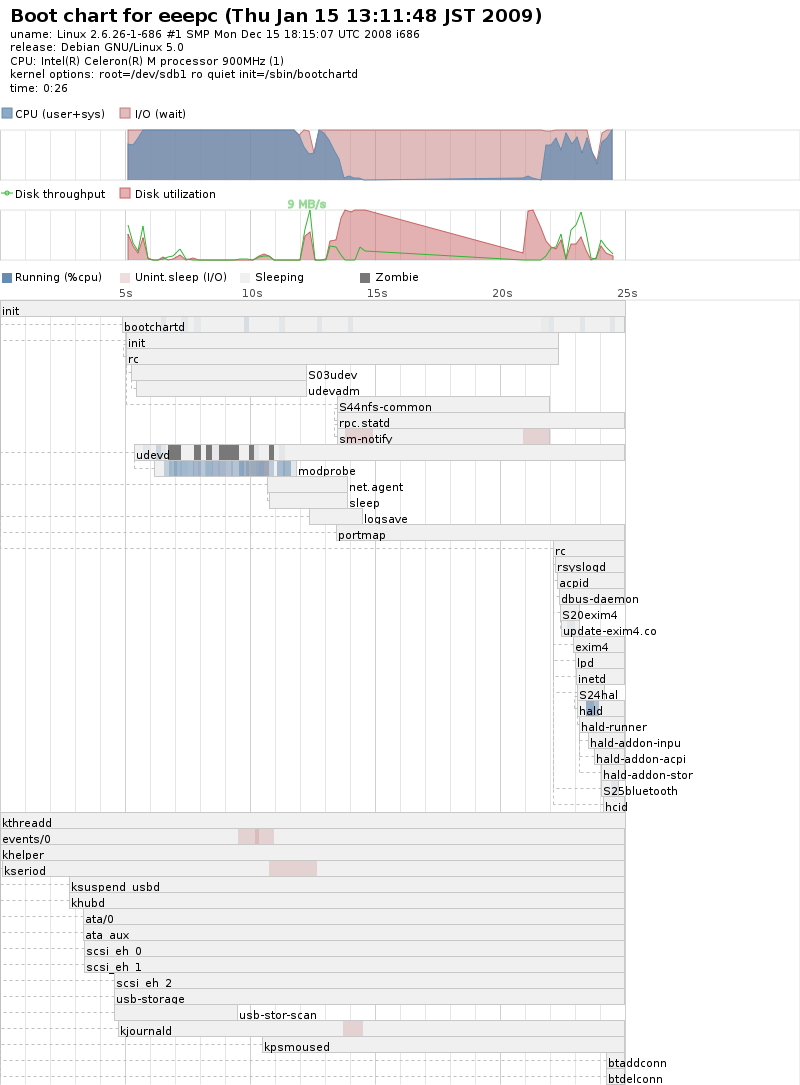
\includegraphics[scale=0.45]{image200901/bootchart-eeepc.png}
     \caption{$BJQ99A0$N(Bbootchart}
     \label{fig:bootchart-eeepc}
     
    \end{center}
   \end{minipage}
   \begin{minipage}{0.5\textwidth}
    \begin{center}
     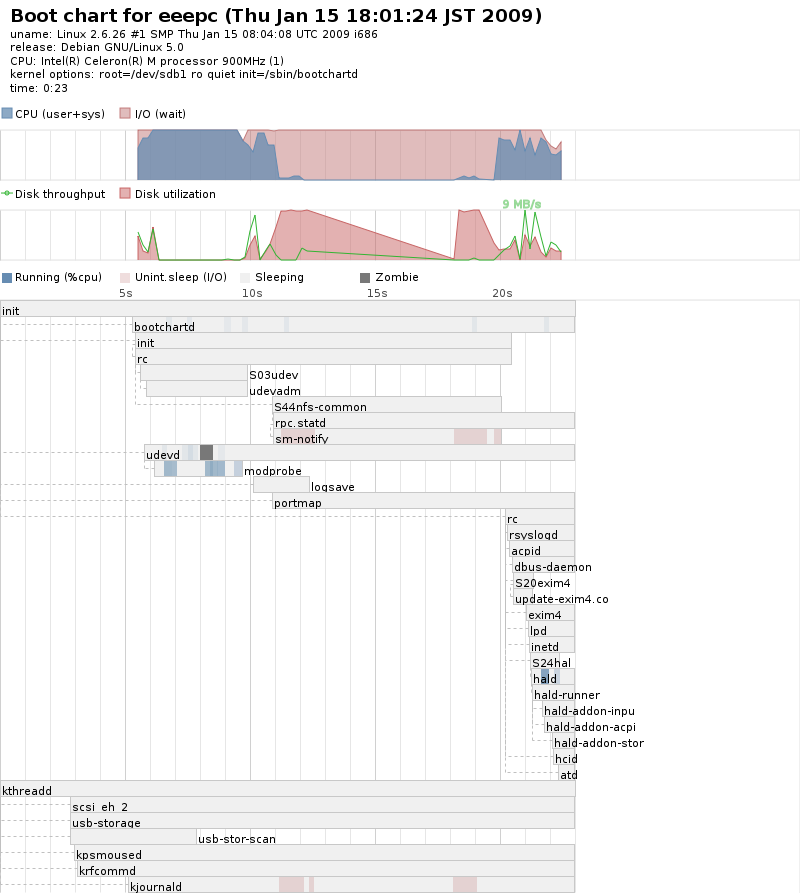
\includegraphics[scale=0.45]{image200901/bootchart-eeepc-new.png}
     \caption{$BJQ998e$N(Bbootchart}
     \label{fig:bootchart-eeepc-new}
    \end{center}
   \end{minipage}
  \end{tabular}
\end{figure}
$B>e$N5/F0%A%c!<%H?^$h$j!"5/F0;~$N%b%8%e!<%k$NFI$_9~$_$,$J$/$J$j!"(B
$B;0IC$[$IB.$/$J$C$F$$$k$3$H$,J,$+$j$^$9!#(B


\subsection{$B:#8e$NM=Dj(B}
$B$3$N%=%U%H%&%'%"$O(BPerl$B$NJY6/$N$?$a$K:n$C$F$_$^$7$?$,!":#8e$NE83+$H$7$F$O(B
$B0J2<$N$3$H$r9M$($F$$$^$9!#(B
\begin{enumerate}
 \item make-kpkg $B$KF~$l$k!)(B

       make-kpkg $B$O(B Perl $B$G:n$i$l$F$$$k$N$GF~$l$d$9$$$+$b$7$l$^$;$s!#(B

 \item $B%Q%C%1!<%82=!)(B

       Debian $B%Q%C%1!<%82=$9$k$H%f!<%6$O4n$V$+$b$7$l$^$;$s!#(B

 \item $B%+!<%M%k%3%s%Q%$%k(BWeb$B%5!<%S%9$NDs6!!)(B

       lsmod $B$N=PNO$,J,$+$l$P(B Debian $B%+!<%M%k$O%3%s%Q%$%k$,MF0W$J$N$G!"(B
       $B%5!<%S%92=$9$k$H%f!<%6$O4n$V$+$b$7$l$^$;$s!#$,!"$=$l$0$i$$<+J,$G(B
       $B$d$l$H$$$&46$8$G$9!#(B

 \item $B%I%i%$%P%*%V%8%'%/%H%U%!%$%k$H%I%i%$%P%b%8%e!<%kL>$,0lCW$7$J$$$d(B
       $B$D$rD>$9!#(B

       $BCN$i$J$$$H%O%^$k$N$G!"0lCW$7$F$*$$$?J}$,$$$$$H;W$C$F$$$^$9!#(B
\end{enumerate}


%============================================================
\dancersection{$B9u(B MacBook $B$N(B Lenny/Sid 64bit $B2=$G$N%O%^$j%]%$%s%H(B}{$B$^$((B
$B$@$3$&$X$$(B}
\index{MacBook}
\index{lilo}
%============================================================

$BG/Kv$N%M%?(B\footnote{2008 $BG/(B 12 $B7n$NJY6/2q$GH/I=$7$?!"%h%a$r(B Debian
GNU/Linux Sid $B%f!<%6$K$9$k!#(B}$B$r<B8=$9$k$?$a$K!"E_5Y$_$rMxMQ$7$F(B 32bit
Sid $B4D6-$@$C$?9u(B MacBook $B$r(B 64bit Sid $B$G:F9=C[$7$^$7$?!#%$%s%9%H!<%k(B
$B<+BN$O$$$D$b$N$H$*$j$N:n6H$J$N$G!"3'$5$s$b$$$D$b$d$C$F$$$i$C$7$c$k$3$H$GLLGr$_$b(B
$B$J$$$N$G$9$,!"G/L@$1$K%j%j!<%9$5$l$F$$$?(B Lenny $B$N(B
Snapshot $B%$%a!<%8$G%V!<%H%m!<%@$K(B LILO $B$rA*Br$7!"%$%s%9%H!<%k8e$K5/F0$5(B
$B$;$k$H(B Kernel Panic $B$K$J$C$F$7$^$$!"$$$-$J$j5/F0$G$-$J$$LdBj$KAx6x$7$^$9!#(B
$B:#2s$O$=$N2sHrJ}K!$K$D$$$F(B\footnote{$B%P%0$N=$@5$G$O$"$j$^$;$s!#?7:'N99TA0(B
$BF|$N?t;~4V$7$+E_5Y$_$O;~4V$r3d$1$^$;$s$G$7$?!D!#(B orz}$B@bL@$7$^$9!#(B


\subsection{$BMQ0U$7$?%$%s%9%H!<%k%$%a!<%8(B}
$B$4B8CN$N$H$*$j!"(BMacBook $B$r(B 64bit $B$G%$%s%9%H!<%k$9$k$K$O!"(B amd64 $BHG$N%$%s(B
$B%9%H!<%k%$%a!<%8$,I,MW$G$9!#:#2s$O!"(B Lenny $B$N%9%J%C%W%7%g%C%H(B
\footnote{Debian GNU/Linux testing "Lenny" - Official Snapshot amd64
NETINST Binary-1 20090104-09:09}$B$r;H$$$^$7$?!#(B

\subsection{$B4JC1$J%$%s%9%H!<%k<j=g(B}
MacBook $B$X$N(B Debian $B$N%$%s%9%H!<%k$K4X$9$k>pJs$O!"2a5n$N(B Debian $BJY6/2q$N(B
$B;qNA$d!"(B Debian Wiki $B$K8x3+$5$l$F$$$^$9!#:#2s$b$=$l$i$HF1MM$N<j=g$G$9!#(B
\begin{enumerate}
\item expert install $B$G$N5/F0!#(B
\item $BF|K\8l%m%1!<%k!"JF9q%-!<%\!<%I$r;XDj!#(B
\item $B%Q!<%F%#%7%g%s$N;XDj$7D>$7!#(B\footnote{LVM $B$G%\%j%e!<%`$r(B
$B:n$C$F$$$k%Q!<%F%#%7%g%s$O%Q!<%F%#%7%g%s$r@Z$jD>$;$J$$LdBj$,$"$j$^$9!#(B}
\item $B4pK\%Q%C%1!<%8$N%$%s%9%H!<%k!#(B
\item $B%7%'%k%b!<%I$X0\9T!#(B
\item gptsync, refit $B%Q%C%1!<%8$N%$%s%9%H!<%k!"(B gptsync $B$N<B9T!#(B
\item apt-line $B$NJQ99!"(Bapt-get \{update,upgrade,dist-upgrade\}$B$N<B9T!#(B
\item $B:F5/F0!#(B
\end{enumerate}

\subsection{$B5/F0$5$;$k$H!D!#(B}
$B<!$N$h$&$J%a%C%;!<%8$rEG$$$F!"(B Kernel Panic $B$K$J$j$^$9!#(B

\begin{commandline}
RAMDISK: Couldn't find valid RAM disk image staring at 0.
List of all partitions:
No filesystem could mount root, tried:
Kernel panic - not syncing: VFS: Unable to mount root fs on unknown-block(8,4)
\end{commandline}

$B<B$O!"%$%s%9%H!<%kD>8e$K(B Kernel Panic $B$H$J$k$N$O:#2s$,=i$a$F$G$O$"$j$^$;$s!#(B MacBook Air
$B$r(B 64bit $B2=$7$?:]$K$bF1$88=>]$,H/@8$7$^$7$?!#(B
\footnote{\url{http://d.hatena.ne.jp/mkouhei/20080713/1215913997}}$B$7$+$7!"(B
MacBook Air $B$N;~$O!"%l%9%-%e!<%b!<%I$G5/F0$7!"(B Kernel $B$r:F9=C[$7$F%$%s%9(B
$B%H!<%k$7$?$i:FH/$7$J$/$J$j$^$7$?!#$H$3$m$,:#2s$O(B Kernel $B$r:F9=C[$7$?$@$1(B
$B$G$O2r7h$G$-$^$;$s!#:$$C$?$b$N$G$9!#(B



\subsection{$B2sHrJ}K!(B}
$B:$$C$?$N$G!"%0%0$C$F$_$?$H$3$m!"F1$88=>]$KBP$7$F$N2sHr:v$b8x3+$5(B
$B$l$F$$$^$7$?!#(B
\footnote{\url{http://linux.derkeiler.com/Mailing-Lists/Debian/2008-11/msg01918.html}}
$B4JC1$K2sHr:v$r$^$H$a$k$H<!$N<j=g$G$9!#(B

\begin{enumerate}
\item $B%l%9%-%e!<%b!<%I$G5/F0$7$^$9!#(B
\item $B%7%'%k%b!<%I$K$J$j!"(B /target $B$X(B chroot $B$7$^$9!#(B
\item $B%+!<%M%k%=!<%9$rE83+$7$^$9!#(B
\item /boot $B0J2<$N3:Ev$N(B kernel config $B$r%+!<%M%k%=!<%9%D%j!<$K%3%T!<$7(B
      $B$^$9!#(B
\item kernel$B$r9=C[$7!"%$%s%9%H!<%k$7$^$9!#(B
\begin{commandline}
REVISION=$(date +%Y%m%d.%H%M)
make-kpkg --initrd --revision $REVISION kernel_image
dpkg -i ../kernel-image-2.6.26_20090105.2330_amd64.deb
\end{commandline}

\item /ramdisk $B%G%#%l%/%H%j$r:n$j(B\footnote{$B%G%#%l%/%H%jL>$OG$0U!#(B/ $BD>2<(B
      $B$K(B $B=jM-<T!"%0%k!<%W$r(B root:root $B$G:n$j$^$9!#(B}$B!"(B initrd $B$rE83+$7$^(B
      $B$9!#(B
\begin{commandline}
mkdir /ramdisk
cd /ramdisk
zcat /boot/initrd-2.6.26 | cpio -i
\end{commandline}

\item $B@h$[$I%$%s%9%H!<%k$7$?(B kernel $B$r%"%s%$%s%9%H!<%k$7$^$9!#(B
\begin{commandline}
dpkg --purge kernel-image-2.6.26
\end{commandline}

\item .config $B$N(B ''INITRAMFS\_SOURCE'' $B$r=q$-49$(!"(B--initrd $B%*%W%7%g%s$J(B
      $B$7$G(B kernel $B$r%j%S%k%I$7$^$9!#(B
\begin{commandline}
sed -i 's:INITRAMFS_SOURCE="":INITRAMFS_SOURCE="/ramdisk":' .config
make-kpkg --revision $REVISION kernel\_image
\end{commandline}

\item $B$G$-$?(B kernel $B%Q%C%1!<%8$r%$%s%9%H!<%k$7$^$9!#(B
\item lilo.conf $B$N(B ''initrd=/initrd.img'' $B$r%3%a%s%H%"%&%H$7!"(Blilo$B$r=q$-(B
      $B9~$_$^$9!#(B

\end{enumerate}

$B$3$l$G!"(Bkernel panic $B$r5/$3$5$:!"$A$c$s$H5/F0$G$-$k$h$&$K$J$j$^$7$?!#$?(B
$B$@$7!":#$N$H$3$m!"?7$?$J%P!<%8%g%s$N(B kernel $B$r9=C[$9$kEY!"F1$8<j=g$rF'$^(B
$B$J$1$l$P$J$j$^$;$s!#(B


\subsection{$B$b$C$H4JC1$J2sHrJ}K!!#(B}
\textbf{ lilo $B$J$s$+$r$d$a$F!"(Bgrub2 $B$K$7$F$7$^$$$^$7$g$&!#(B}
$B$*$"$H$,$h$m$7$$$h$&$G!#(B

% from debianmeetingresume200902.tex
\dancersection{Debian $B%Q%C%1!<%8%s%0%O%s%:%*%s$N<j0z=q(B}{$B4d>>(B $B?.MN(B}
%\section{Debian $B%Q%C%1!<%8%s%0%O%s%:%*%s$N<j0z=q(B}
\subsection{$BK\F|$NL\E*(B}
Debian$B%Q%C%1!<%82=$5$l$F$$$J$$%=%U%H%&%'%"$r%Q%C%1!<%82=$7$F!"(B
$B%S%k%I%F%9%H$H%Q%C%1!<%8$NJQ99$^$G$rBN83$7$^$9!#(B
$B$H$3$m$I$3$m$K%H%i%C%W$,$"$k$N$GCm0U$7$^$7$g$&!#(B
\subsection{$BK\F|$NN.$l(B}
\begin{enumerate}
\item $B9V;U>R2p(B
\item $B:n6H$r;O$a$kA0$NA0=`Hw(B
\item $B%=%U%H%&%'%"$N%3%s%Q%$%k(B
\item $B%Q%C%1!<%8$N?w7A(B
\item CDBS
\item debian$B%G%#%l%/%H%j0J2<%U%!%$%k$NJT=8(B
\item $B%Q%C%1!<%8$N%S%k%I(B
\item $B%Q%C%1!<%8$N%$%s%9%H!<%k(B
\item $B%Q%C%1!<%8$N%S%k%I%F%9%H(B
\item $B%Q%C%1!<%8$N%$%s%9%H!<%k(B/$B%"%s%$%s%9%H!<%k%F%9%H(B
\item $B%W%m%0%i%`$NJT=8(B
\item $B<A5?1~Ez(B
\end{enumerate}


\subsection{$B5-9f$N@bL@(B}
{\bf \$} $B$,IU$$$F$$$k>l9g$O!"%3%s%=!<%k$+$i$NF~NO$r0UL#$7$^$9!#(B{\bf \$}$B$OF~NO$;$:$K(B
$B%3%^%s%I$rF~NO$7$F$/$@$5$$!#(B

$B%3%^%s%I%i%$%s$d%U%!%$%k$NCf?H$G(B{\bf \textbackslash}$B$,=q$+$l$F$$$k>l=j$O9T$,B3$$$F(B
$B$$$k;v$r0UL#$7$^$9!#F~NO$7$J$$$G$/$@$5$$!#(B 

{\bf ...}$B$O>JN,$r0UL#$7$^$9!#<B:]$K$OD9$$=PNO$,$"$k>l9g$K>JN,$7$F$$$k>l(B
$B9g$KMxMQ$7$F$$$^$9!#(B

\subsection{$B%(%G%#%?(B}
$BK\%O%s%:%*%s$G$O!"%(%G%#%?$H$7$F(B{\bf vi}$B$*$h$S(B{\bf mousepad}$B$r;H$($k$h$&$K$7$F$$(B
$B$^$9!#(B{\bf vi}$B$,;H$($J$$?M$O!"(B{\bf mousepad}$B$r;H$C$F$/$@$5$$!#(BWindows$B$N%a%bD"$H(B
$BF1$85!G=$r;}$C$?%(%G%#%?$G$9!#(B

\subsection{$B%k!<%H8"8B$K$D$$$F(B}
$BK\%O%s%:%*%s$G$O!"(Broot$B8"8B$r;H$C$?:n6H$r9T$&>l9g$,$"$j$^$9!#(B
$B$=$N>l9g$K$O(B sudo $B%3%^%s%I$r;H$C$F:n6H$r$7$^$9!#(B{\bf sudo}$B%3%^%s%I$,I,MW$J>l(B
$B9g$K$O%3%^%s%I%i%$%s$N@bL@$N$H$3$m$K(B{\bf sudo}$B$r;XDj$7$F$$$^$9!#(B

\subsection{$BA0=`Hw(B} 
\subsubsection{$B%Q%C%1!<%8%a%s%F%JL>$N@_Dj(B}
$B%Q%C%1!<%8%a%s%F%J$NL>A0$H%a!<%k%"%I%l%9$r4D6-JQ?t$K@_Dj$7$^$9!#(B
$BE,Ev$J$G%(%G%#%?$r;H$C$F!"(B{\bf /home/user/.bashrc} $B$K0J2<$NNc$N$h$&$KJQ(B
$B99$7$FJ]B8$7$F$/$@$5$$!#3F9`L\$K$O<+J,$NL>A0$H%a!<%k%"%I%l%9$r$$$l$F$/$@(B
$B$5$$!#(B
\begin{commandline}
export DEBFULLNAME="Nobuhiro Iwamatsu"
export DEBEMAIL=iwamatsu@nigauri.org
\end{commandline}
$BJ]B8$G$-$?$i!"%?!<%_%J%k$r5/F0$7!"(B
\begin{commandline}
$ source ~/.bashrc
\end{commandline}
$B$r<B9T$7$F$/$@$5$$!#(B

\subsubsection{web$B%5!<%P$NN)$A>e$2(B}
$B%3%s%=!<%k$+$i0J2<$N%3%^%s%I$r<B9T$7$F$/$@$5$$!#$3$l$O(BLive-CD$B4D6-$G(B
apt-get$B$,$G$-$k$h$&$K$9$k$?$a$NBP:v$H$7$F9T$C$F$$$^$9!#<B:]$N%Q%C%1!<%8(B
$B:n@.$G$OI,MW$"$j$^$;$s!#(B
\begin{commandline}
$ sudo ruby1.8 ./tools/web.rb
\end{commandline}

\subsubsection{apt-line$B$NJQ99(B}
$B%(%G%#%?$r;H$$!"(B{\bf /etc/apt/sources.list}$B%U%!%$%k$r0J2<$N$h$&$KJQ99$7$F$/$@$5$$!#(B
apt-line $B$,=q$+$l$F$$$^$9$,!":o=|$7$F$/$@$5$$!#(B
\begin{commandline}
deb http://localhost/debian lenny main
\end{commandline}

\subsubsection{$B%j%]%8%H%j>pJs$N%"%C%W%G!<%H(B}
$B%j%]%8%H%j$N%"%C%W%G!<%H$r9T$$$^$9!#0J2<$N$h$&$K%3%^%s%I$r<B9T$7$^$9!#(B
\begin{commandline}
$ sudo apt-get update
\end{commandline}

\subsubsection{/tmp $B$N%^%&%s%H%*%W%7%g%s$NJQ99(B}
{\bf /tmp}$B$r(B{\bf nodev}$B%*%W%7%g%s$J$7$G(B{\bf remount}$B$7$^$9!#(B
$B0J2<$N$h$&$K<B9T$7$^$9!#(B
\begin{commandline}
sudo mount -o remount,dev /tmp
\end{commandline}

\subsection{$B:#2s$N%5%s%W%k(B}
$B:#2s$O!"(B{\bf cwidget}$B$r;H$C$?%5%s%W%k%W%m%0%i%`(B
{\bf /live/image/osc/data/hello-cwidget-0.1.tar.gz}
$B$rMQ0U$7$^$7$?!#(B
$B$3$N%5%s%W%k%W%m%0%i%`$r(BDebian$B%Q%C%1!<%82=$7$^$9!#(B
{\bf /live/image/osc/data}$B%G%#%l%/%H%j$K%=!<%9%U%!%$%k$,$"$k$N$G!"%[!<%`%G%#%l%/%H%j$KE83+$7$^$9!#(B
\begin{commandline}
$ cd
$ tar -xzf /live/image/osc/data/hello-cwidget-0.1.tar.gz
\end{commandline}
\footnote{$B$3$N%U%!%$%k$O(B\url{http://www.nigauri.org/~iwamatsu/trash/hello-cwidget-0.1.tar.gz}$B$+$i%@%&%s%m!<%I2DG=$G$9!#(B}

$B$3$N%=%U%H%&%'%"$O(B C++ $B$G5-=R$5$l$F$*$j!"%3%s%Q%$%k$KI,MW$J%i%$%V(B
$B%i%j$d%=%U%H%&%'%"$,%$%s%9%H!<%k$5$l$F$$$k>l9g$K$O!"(B./configure ; make ;
make install $B$G%3%s%Q%$%k$*$h$S%$%s%9%H!<%k$^$G$,$G$-$k$h$&$K$J$C$F$$$^(B
$B$9!#(B

\subsection{$B%Q%C%1!<%8%s%02=3+;O(B}
\subsubsection{$B%=!<%9$rFI$s$G$_$k(B}
$BF0:n$7$J$$%W%m%0%i%`$r%Q%C%1!<(B
$B%82=$7$F$b$7$g$&$,$J$$$N$G!"@h$K$I$N$h$&$J%=%U%H%&%'%"$J$N$+M}2r$9$k$?$a(B
$B$K$b%Q%C%1!<%8%s%02=$9$kA0$K%=!<%9%3!<%I$rFI$s$G!"%=%U%H%&%'%"$NCf?H$rM}(B
$B2r$7$FCV$-$^$7$g$&!#(B

\subsubsection{$B$H$j$"$($:!"%3%s%Q%$%k$7$F$_$k(B}
$BF0$+$J$$%W%m%0%i%`$r%Q%C%1!<%82=$7$F$b$7$g$&$,$J$$$N$G!"F0:n3NG'$r$7$^$9!#(B
$B$^$:$O:GDc8B%3%s%Q%$%k$KI,MW$J%Q%C%1!<%8$r%$%s%9%H!<%k$9$kI,MW(B
$B$,$"$j$^$9!#$=$l$,(B{\bf build-essential}$B%Q%C%1!<%8$G$9!#$3$l$O!"%Q%C%1!<(B
$B%82=$N>l9g$K$bI,MW$G$9!#0J2<$N$h$&$K<B9T$7!"%$%s%9%H!<%k$7$^$9!#(B
\begin{commandline}
$ sudo apt-get install build-essential
\end{commandline}

$B@h$[$I2rE`$7$?%G%#%l%/%H%j$K0\F0$7$^$9!#0\F0$7$?$i!"(B{\bf configure}$B$r<B(B
$B9T$7$^$9!#(B
\begin{commandline}
$ cd hello-cwidget-0.1
$ ./configure
...
Alternatively, you may set the environment variables \
SIGC_CFLAGS
and SIGC_LIBS to avoid the need to call pkg-config.
See the pkg-config man page for more details.
...
\end{commandline}
$B<B9T$9$k$H!"%(%i!<$K$J$j$^$9!#(B
\subsection{$BI,MW$J%i%$%V%i%j$rC5$9(B}
Debian$B$GFCDj$N%U%!%$%k$,Ds6!$5$l$F$$$k%Q%C%1!<%8$rC5$9>l9g$K$O!"(B
{\bf apt-file}$B$rMxMQ$7$^$9!#0J2<$N$h$&$K<B9T$7!"%$%s%9%H!<%k$7$^$9!#(B
\begin{commandline}
$ sudo apt-get install apt-file
\end{commandline}
$BDL>o$O!"(B $B$3$N8e!"(B{\bf apt-file update}$B$r<B9T$7!"%U%!%$%k>pJs%G!<%?$r<hF@$7$^$9$,!"(B
$B4{$K(BLive-CD$B$KF~$l$F$$$k$N$G>JN,$7$^$9!#%U%!%$%k$rC5$9$K$O0J2<$N$h$&$K<B9T$7$^$9!#(B
\begin{commandline}
$ apt-file search pkg-config
...
nant: /usr/share/doc/nant/help/functions/pkg-config.\
     is-max-version.html
pkg-config: /usr/bin/pkg-config
pkg-config: /usr/share/doc/pkg-config/AUTHORS
...
\end{commandline}
$B<B9T$9$k$H!";XDj$7$?%U%!%$%k$rDs6!$7$F$$$k%Q%C%1!<%8L>$,=PNO$5$l$^$9!#(B
$B=PNO$5$l$?%Q%C%1!<%8$r%$%s%9%H!<%k$7$^$9!#(B

\begin{commandline}
$ sudo apt-get install pkg-config
\end{commandline}

$B:FEY(B{\bf configure}$B$r<B9T$7$F$_$^$7$g$&!#(B
\begin{commandline}
$ ./configure
...
No package 'sigc++-2.0' found

Consider adjusting the PKG_CONFIG_PATH environment variable if you
installed software in a non-standard prefix.
...
\end{commandline}
$B$^$@B-$j$J$$%Q%C%1!<%8$,$"$k$h$&$G$9!#@h$[$I$HF1$8$h$&$K(B{\bf apt-file}$B$r(B
$BMxMQ$7$F8!:w$7!"%$%s%9%H!<%k$7$^$9!#(B

\begin{commandline}
$ apt-file search sigc++-2.0.pc
libsigc++-2.0-dev: /usr/lib/pkgconfig/sigc++-2.0.pc
$ sudo apt-get install libsigc++-2.0-dev 
\end{commandline}
$B:FEY(B configure $B$r<B9T$7$^$9!#(B
\begin{commandline}
$ ./configure
...
checking for CWIDGET... configure: error: Package \
  requirements(cwidget) were not met:

No package 'cwidget' found

Consider adjusting the PKG_CONFIG_PATH environment variable \
if you
installed software in a non-standard prefix.
...
\end{commandline}
$B%(%i!<$K$J$j$^$9!#$^$@B-$j$J$$$h$&$J$N$G!":FEY8!:w$7$F%$%s%9%H!<%k$7$^$9!#(B

\begin{commandline}
$ apt-file search cwidget.pc
libcwidget-dev: /usr/lib/pkgconfig/cwidget.pc
$ sudo apt-get install libcwidget-dev
\end{commandline}

\begin{commandline}
./configure
...
config.status: WARNING:  Makefile.in seems to ignore the \
   --datarootdir setting
config.status: creating src/Makefile
config.status: WARNING:  src/Makefile.in seems to ignore the \
  --datarootdir setting
config.status: creating config.h
\end{commandline}

{\bf configure}$B$,@5>o$K=*N;$7$^$7$?!#=*N;$9$k$H!"(B{\bf Makefile}$B$,(B
$B:n@.$5$l$F$$$^$9!#(B{\bf make}$B$r<B9T$7!"%3%s%Q%$%k$7$^$9!#(B
\begin{commandline}
$ make
...
make[1]: $B%G%#%l%/%H%j(B `/home/user/hello-cwidget-0.1' \
$B$KF~$j$^$9(B
Making all in src
make[2]: $B%G%#%l%/%H%j(B `/home/user/hello-cwidget-0.1/src' \
$B$KF~$j$^$9(B
g++ -DHAVE_CONFIG_H -I. -I. -I..     -g -O2 -I/usr/ \
include/sigc++-2.0 \
-I/usr/lib/sigc++-2.0/include   -I/usr/lib/cwidget
 -I/usr/include/sigc++-2.0  -I/usr/lib/sigc++-2.0/include \
 -c hello.cc
g++  -g -O2 -I/usr/include/sigc++-2.0 -I/usr/lib/ \
sigc++-2.0/include   \
-I/usr/lib/cwidget -I/usr/include/sigc++-2.0
-I/usr/lib/sigc++-2.0/include \
-o hello  hello.o  -lsigc-2.0   -lcwidget -lncursesw \
-lsigc-2.0  
make[2]: $B%G%#%l%/%H%j(B `/home/user/hello-cwidget-0.1/src' \
$B$+$i=P$^$9(B
make[2]: $B%G%#%l%/%H%j(B `/home/user/hello-cwidget-0.1' $B$KF~$j$^$9(B
make[2]: $B%G%#%l%/%H%j(B `/home/user/hello-cwidget-0.1' $B$+$i=P$^$9(B
make[1]: $B%G%#%l%/%H%j(B `/home/user/hello-cwidget-0.1' $B$+$i=P$^$9(B
\end{commandline}

$B%3%s%Q%$%k$b@5>o$K=*N;$7$?$N$G!";n$7$K<B9T$7$F$_$^$9!#(B
\begin{commandline}
$ ./src/hello
\end{commandline}

$B$3$3$^$G$O%5%s%W%k%W%m%0%i%`$NF0:n3NG'$G$9!#F0:n$7$J$$%W%m%0%i%`$r%Q%C%1!<(B
$B%82=$7$F$b$7$g$&$,$J$$$N$G!"@h$K$I$N$h$&$J%=%U%H%&%'%"$J$N$+M}2r$9$k$?$a(B
$B$K$b%Q%C%1!<%8%s%02=$9$kA0$K%=!<%9%3!<%IEy$rFI$s$G$*$/$3$H$r$*4+$a$7$^$9!#(B

\subsection{Deban$B%Q%C%1!<%8$N?w7A(B}
{\bf dh\_make}$B%3%^%s%I$G%Q%C%1!<%8$N?w7A$r:n@.$9$k$3$H$,$G$-$^$9!#(B
{\bf dh\_make}$B$O!"(B{\bf dh-make}$B%Q%C%1!<%8$GDs6!$5$l$F$$$^$9!#(B
$B0J2<$N%3%^%s%I$r<B9T$7!"%$%s%9%H!<%k$7$^$9!#(B
\begin{commandline}
$ sudo apt-get install dh-make
\end{commandline}

$B?w7A$N:n@.$O0J2<$N%3%^%s%I$r<B9T$7$^$9!#(B
\begin{commandline}
$ dh_make --createorig -s
\end{commandline}
{\bf --createorig}$B%*%W%7%g%s$O%*%j%8%J%k%=!<%9%3!<%I$N(Btar.gz$B%$%a!<%8$r9=C[$7(B
  $B$^$9!#(B $B:#2s$O%7%s%0%k%P%$%J%j%Q%C%1!<%8!J0l$D$N%=!<%9%3!<%I$+$i0l$D$N(B
  $B%P%$%J%j%Q%C%1!<%8$,:n@.$5$l$k!K$J$N$G(B{\bf -s} $B$r;XDj$7$^$9!#<B9T$9$k$H0J2<(B
  $B$N$h$&$J%a%C%;!<%8$,I=<($5$l$k$N$G!"(BEnter$B%-!<$r2!$7$^$9!#(B
\begin{commandline}
Maintainer name : Nobuhiro Iwamatsu
Email-Address   : iwamatsu@nigauri.org 
Date            : Sun, 15 Feb 2009 23:51:58 +0900
Package Name    : hello-cwidget
Version         : 0.1
License         : blank
Using dpatch    : no
Using quilt     : no
Type of Package : Single
Hit <enter> to confirm: 
\end{commandline}

\subsubsection{debian$B%G%#%l%/%H%j(B}
$B$&$^$/F0:n$9$k$H!"(B{\bf debian$B%G%#%l%/%H%j(B}$B$,:n@.$5$l!"$3$NCf$K?w7A$,:n@.$5$l(B
$B$^$9!#%Q%C%1!<%8%a%s%F%J$O$3$N%G%#%l%/%H%j$NCf0J30$O?($j$^$;$s!#(B
$B0J2<$N$h$&$J>uBV$K$J$C$F$$$^$9!#(B
\begin{commandline}
.
|-- README.Debian  (Debian$B%Q%C%1!<%8$N(B README)
|-- changelog      (Debian$B%Q%C%1!<%8$N%A%'%s%8%m%0(B)
|-- compat         (Debian$B%Q%C%1!<%8$N%P!<%8%g%s(B)
|-- control        (Debian$B%Q%C%1!<%8>pJs(B)
|-- copyright      ($B%3%T!<%i%$%H>pJs(B)
|-- cron.d.ex      (cron $B$r;H$&%Q%C%1!<%8MQ@_Dj%U%!%$%k(B)
|-- dirs           ($B:n@.$9$k%G%#%l%/%H%jL>$r;XDj$9$k(B)
|-- docs           ($B%$%s%9%H!<%k$9$k%I%-%e%a%s%H%U%!%$%k$r;XDj$9$k(B)
|-- emacsen-install.ex (emacs $BMQ@_Dj%U%!%$%k(B)
|-- emacsen-remove.ex  (emacs $BMQ@_Dj%U%!%$%k(B)
|-- emacsen-startup.ex (emacs $BMQ@_Dj%U%!%$%k(B)
|-- hello-cwidget.default.ex (debfonf$BMQ(B)
|-- hello-cwidget.doc-base.EX (doc-base$BMQ(B)
|-- init.d.ex      (init.d$B$r;H$&%Q%C%1!<%8MQ@_Dj%U%!%$%k(B)
|-- init.d.lsb.ex  (init.d$B$r;H$&%Q%C%1!<%8MQ@_Dj%U%!%$%k(B)
|-- manpage.1.ex   (manpage $B$N?w7A(B)
|-- manpage.sgml.ex(manpage $B$N?w7A(B)
|-- manpage.xml.ex (manpage $B$N?w7A(B)
|-- menu.ex        ($B%a%K%e!<$N?w7A(B)
|-- postinst.ex    (postinst$B%a%s%F%J%U%!%$%k$N?w7A(B)
|-- postrm.ex      (postrm$B%a%s%F%J%U%!%$%k$N?w7A(B)
|-- preinst.ex     (preinst$B%a%s%F%J%U%!%$%k$N?w7A(B)
|-- prerm.ex       (prerm$B%a%s%F%J%U%!%$%k$N?w7A(B)
|-- rules          ($B%Q%C%1!<%8%S%k%I%9%/%j%W%H(B)
`-- watch.ex       ($B%"%C%W%9%H%j!<%`%A%'%C%/MQ%U%!%$%k(B)
\end{commandline}

\subsection{CDBS}
./configure ; make ; make install $B$G%Q%C%1!<%8$N%3%s%Q%$%k$,$G$-$k(B
$B%=%U%H%&%'%"$O(B cdbs $B$r;H$C$?J}$,MF0W$K(BDebian$B%Q%C%1!<%82=$G$-$^$9!#(B


\subsubsection{$B0l2s(B hello-cwidget$B%G%#%l%/%H%j$r:o=|$9$k(B}
$B8=>u$G$O@h$[$I$N(B{\bf dh\_make}$B$N7k2L$,;D$C$F$$$k$N$G0l2s!"%5%s%W%k%W%m%0(B
$B%i%`$N%G%#%l%/%H%j$4$H:o=|$7!":FEYE83+$7$^$9!#(B
\begin{commandline}
$ cd 
$ rm -rf hello-cwidget-0.1.*
$ tar -xzf /live/image/osc/data/hello-cwidget-0.1.tar.gz
$ cd hello-cwidget-0.1
\end{commandline}

\subsubsection{dh\_make$B$r<B9T$7!"%Q%C%1!<%8$N?w7A$r:n@.$9$k(B}

{\bf CDBS}$B$r;H$&(BDebian$B%Q%C%1!<%8$N?w7A:n@.$O0J2<$N%3%^%s%I$r<B9T$7$^$9!#(B
\begin{commandline}
$ dh_make --createorig -b
\end{commandline}
{\bf -b}$B%*%W%7%g%s$r;XDj$9$k$H!"(BCDBS $B$r;H$C$??w7A$r:n@.$7$^$9!#(B
$B0J2<$N$h$&$J%a%C%;!<%8$,I=<($5$l$k$N$G!"%(%s%?!<%-!<$r2!$7$^$9!#(B
\begin{commandline}
Maintainer name : Nobuhiro Iwamatsu
Email-Address   : iwamatsu@nigauri.org 
Date            : Sun, 15 Feb 2009 23:51:58 +0900
Package Name    : hello-cwidget
Version         : 0.1
License         : blank
Using dpatch    : no
Using quilt     : no
Type of Package : cdbs
Hit <enter> to confirm: 
\end{commandline}

\subsubsection{$BITMW$J%U%!%$%k$N:o=|(B}
$B:#2s$N%Q%C%1!<%82=$KI,MW$G$O$J$$%U%!%$%k$r(B{\bf debian}$B%G%#%l%/%H%j0J2<$+$i:o=|(B
$B$7$^$9!#(B
\begin{commandline}
$ rm -rf debian/*.ex debian/*.EX
\end{commandline}

\subsubsection{debian/changelog$B%U%!%$%k$NJT=8(B}
{\bf debian/changelog}$B%U%!%$%k$K$O(B{\bf ITP}(Intent To Package)
$B$N%P%0$,4{$K=q$+$l$F$$$k$G:o=|$7$^$9!#0J2<$N$h$&$KJQ99$7$^$9!#(B
\begin{commandline}
hello-cwidget (0.1-1) unstable; urgency=low

  * Initial release.

 -- Nobuhiro Iwamatsu <iwamatsu@nigauri.org> \
                  Wed, 18 Feb 2009 16:31:25 +0000

\end{commandline}
\subsubsection{debian/copyright$B%U%!%$%k$NJT=8(B}
\begin{commandline}
This package was debianized by Nobuhiro Iwamatsu \ 
                                <iwamatsu@nigauri.org> on
Wed, 18 Feb 2009 16:31:25 +0000.

It was downloaded from <http://www.nigauri.org/~iwamatsu/>

Upstream Author:

    Nobuhiro Iwamatsu <iwamatsu@nigauri.org>

Copyright:

    Copyright (C) 2009 Nobuhiro Iwamatsu <iwamatsu@nigauri.org>

License:

    GPLv2

The Debian packaging is (C) 2009, Nobuhiro Iwamatsu \ 
        <iwamatsu@nigauri.org> and
is licensed under the GPL, see `/usr/share/common-licenses/GPL'.
\end{commandline}
\subsubsection{debian/control$B%U%!%$%k$NJT=8(B}
\begin{commandline}
Source: hello-cwidget
Section: devel
Priority: extra
Maintainer: Nobuhiro Iwamatsu <iwamatsu@nigauri.org>
Build-Depends: cdbs, debhelper (>= 7), autotools-dev
Standards-Version: 3.8.0
Homepage: http://www.nigauri.org/~iwamatsu/

Package: hello-cwidget
Architecture: any
Depends: ${shlibs:Depends}, ${misc:Depends}
Description: Debian Packaging Hands-on sample program
 This is sample program of Debian Hands-on done with
 OSC2009 TOKYO Spring.
 This is very easy program that uses CWidget.
\end{commandline}

\subsubsection{$B%Q%C%1!<%8$N%S%k%I(B}

$B%Q%C%1!<%8$N%S%k%I$K$O(B{\bf debuild}$B%3%^%s%I(B $B$r;H$$$^$9!#(B
debuild$B%3%^%s%I$O(B{\bf devscripts}$B%Q%C%1!<%8$GDs6!$5$l$F$$$^$9!#(B
$B$^$?!"$^$@(B {\bf CDBS}$B%Q%C%1!<%8$r%$%s%9%H!<%k$7$F$$$J$$$N$G!"0l=o$K%$%s(B
$B%9%H!<%k$7$^$9!#(B
$B%Q%C%1!<%8$r%$%s%9%H!<%k$7$?$i!"%Q%C%1!<%8$N%S%k%I$r$7$F$_$^$7$g$&!#(B
\begin{commandline}
$ sudo apt-get install devscripts cdbs
$ debuild -us -uc
...
dpkg-buildpackage: full upload (original source is included)
Now running lintian...
W: hello-cwidget: binary-without-manpage usr/bin/hello
W: hello-cwidget: new-package-should-close-itp-bug
Finished running lintian.
\end{commandline}

\subsection{$B%Q%C%1!<%8$N%$%s%9%H!<%k(B}
$B%Q%C%1!<%8$,L5;v%S%k%I$G$-$?$i!"<B:]$K%$%s%9%H!<%k$7$F$_$^$9!#(B
$B%$%s%9%H!<%k$K$O(B dpkg $B%3%^%s%I$r;H$C$F%$%s%9%H!<%k$7$^$9!#%$%s%9%H!<%k$7(B
$B$?$i!"<B:]$KF0$/$+3NG'$7$F$_$^$7$g$&!#(B
\begin{commandline}
$ sudo dpkg -i ../hello-cwidget_0.1-1_i386.deb
$ which hello
$ hello
\end{commandline}

\subsection{$B%Q%C%1!<%8$N%S%k%I%F%9%H(B}
$B%Q%C%1!<%8$,$G$-$?$"$H$K$O%Q%C%1!<%8$N%F%9%H$r9T$$$^$9!#(B
$B%Q%C%1!<%8$N%S%k%I%F%9%H$K$O(B{\bf pbuilder}$B$r;H$$$^$9!#(B
pbuilder$B$O(BDebian$B$KI,MW$J:GDc8B$N4D6-$+$i%S%k%I$r9T$$!"(B
$B0MB84X78Ey$N%A%'%C%/$r9T$C$F%S%k%I%F%9%H$r9T$&%D!<%k$G$9!#(B

\subsubsection{pbuilder$B%Q%C%1!<%8$N%$%s%9%H!<%k(B}
\begin{commandline}
$ sudo apt-get install pbuilder
\end{commandline}

\subsubsection{pbuilder$B4D6-$N9=C[(B}

$B%S%k%I%F%9%H$r9T$&A0$K(Bbase$B%7%9%F%`%$%a!<%8$r9=C[$9$kI,MW$,$"$j$^$9!#(B
$BDL>o$O0J2<$N$h$&$K<B9T$7$^$9$,!"(B
\begin{commandline}
$ sudo pbuilder --create --distribution lenny
\end{commandline}
$B:#2s$O%a%b%j$N@)8B$,$"$k$?$a!"4{$KMQ0U$7$F$"$k(Bbase$B%7%9%F%`%$%a!<%8$rMxMQ(B
$B$7$^$9!#%$%a!<%8$O(B{\bf /live/image/osc/data/base.tgz}$B$K$"$j$^$9!#(B

\subsubsection{$B%Q%C%1!<%8$N%S%k%I%F%9%H(B}

pbuilder $B$G%F%9%H$9$k>l9g$K$O:n@.$5$l$?%Q%C%1!<%8$N(B{\bf dsc}$B%U%!%$%k$r;XDj$7(B
$B$^$9!#$3$N%U%!%$%k$K$O!"(BDebian$B%Q%C%1!<%8$N9=@.$KI,MW$J%U%!%$%kL>$,=q$+$l(B
$B$F$$$k$N$G!"$=$N>pJs$r85$K:F%S%k%I$r9T$&$3$H$,$G$-$^$9!#(B
$B$^$?!"<B9TA0$K(B{\bf apt-get clean}$B%3%^%s%I$r<B9T$7$F%-%c%C%7%e$r%/%j%"$7(B
$B$F$/$@$5$$!#%a%b%j$,B-$j$J$$$?$a$G$9!#(B
\begin{commandline}
$ cd ..
$ sudo apt-get clean
$ sudo pbuilder --build --distribution lenny \ 
     --basetgz /live/image/osc/data/base.tgz \
     --buildplace /tmp hello-cwidget_0.1-1.dsc
...
\end{commandline}

\subsubsection{$B$J$<%(%i!<$K$J$k$N$+(B}
$B@h$[$I$N<j=g$G$d$C$F$b%S%k%I%(%i!<$K$J$j$^$9!#(B
$B$J$<%(%i!<$K$J$k$N$G$7$g$&$+!#9M$($F$_$^$7$g$&!#(B

\subsubsection{$B:F%S%k%I%F%9%H(B}
$B%(%i!<$K$J$kM}M3$O@h$K%$%s%9%H!<%k$7$?%Q%C%1!<%8(B{\bf libcwidget-dev}$B$r%Q%C%1!<(B
$B%8%S%k%I;~$N0MB84X78$r5-=R$9$k%U%#!<%k%I(B{\bf Build-Depends}$B$KDI2C$7$F$$(B
$B$J$$$?$a$G$9!#DI2C$7$F!":F%S%k%I$7$F$_$^$9!#(B
$B:F%S%k%I$K$O0J2<$N$h$&$K<B9T$7$^$9!#:#EY$O$&$^$/%S%k%I$,$G$-$k$O$:$G$9!#(B
\begin{commandline}
$ sudo pdebuild -- --distribution lenny --basetgz \
 /live/image/osc/data/base.tgz --buildplace /tmp
\end{commandline}


\subsection{$B%Q%C%1!<%8$N%$%s%9%H!<%k(B/$B%"%s%$%s%9%H!<%k%F%9%H(B}
$B%Q%C%1!<%8$,%S%k%I$G$-$?$@$1$G$O4n$s$G$O$$$1$^$;$s!#%$%s%9%H!<%k(B/$B%"%s%$(B
$B%s%9%H!<%k$N%F%9%H$b9T$$$^$7$g$&!#(B
$B%Q%C%1!<%8$N%$%s%9%H!<%k(B/$B%"%s%$%s%9%H!<%k$N%F%9%H$K$O(B{\bf piuparts}$B%Q%C(B
$B%1!<%8$r;H$$$^$9!#(B
\subsubsection{piuparts$B$N%$%s%9%H!<%k(B}
$B0J2<$N$h$&$K<B9T$7!"%$%s%9%H!<%k$7$^$9!#(B
\begin{commandline}
$ sudo apt-get install piuparts
\end{commandline}

\subsubsection{$B%Q%C%1!<%8$N%$%s%9%H!<%k(B/$B%"%s%$%s%9%H!<%k%F%9%H(B}
piuparts$B$b(Bpbuilder$B$HF1MM$K:GDc8B$N4D6-$+$i$N%$%s%9%H!<%k$r%A%'%C%/$7$^$9!#(B
$B$h$C$F!"(Bbase$B%7%9%F%`%$%a!<%8$,I,MW$G$9!#IaCJ$O;XDj$9$kI,MW$O$"$j$^$;$s$,!"(B
$B:#2s$O(B{\bf -b}$B%*%W%7%g%s$rIU$1$F!"(B{\bf /live/image/osc/data/base.tgz}$B$K(B
$B$"$k(Bbase$B%7%9%F%`%$%a!<%8$r;XDj$7$F<B9T$7$^$9!#(B
\begin{commandline}
$ cd ..
$ sudo piuparts -d lenny -b /live/image/osc/data/base.tgz \
   hello-cwidget_0.1-1_i386.deb
...
0m41.9s DEBUG: Removed directory tree at /tmp/tmpHliOKO
0m41.9s INFO: PASS: All tests.
0m41.9s INFO: piuparts run ends.
\end{commandline}

\subsection{$B%W%m%0%i%`$NJT=8(B}
hello-cwidget$B$r<B9T$7$F!"0cOB46$N$"$kJ}$,$*$i$l$?$H;W$$$^$9!#(B
$B$=$&!"(B{\bf Lenny}$B$,%j%j!<%9$5$l$?$H$$$&$N$K(B{\bf Etch}$B$K$J$C$F$$$^$7$?!#(B
$B$3$l$O$h$/$J$$$N$GJQ99$7$F$_$^$9!#:#2s$O$h$/MxMQ$5$l$F$$$k(B{\bf dpatch}
$B$r;H$C$F@bL@$7$^$9!#(B
\subsubsection{dpatch$B$N%$%s%9%H!<%k(B}
dpatch$B$r%$%s%9%H!<%k$9$k$K$O!"0J2<$N$h$&$K<B9T$7$^$9!#(B
\begin{commandline}
$ sudo apt-get install dpatch
\end{commandline}
\subsubsection{dpatch$B$r;H$&$?$a$N=`Hw(B}
dpatch$B$r;H$&A0$K!"(B{\bf debian/rules}$B%U%!%$%k$K(Bdpatch$B$r;H$&$h$&$K@_Dj$9$kI,MW$,(B
$B$"$j$^$9!#(Bdpatch$B$O0l2s!"%Q%C%1!<%8$N>uBV$r=i4|2=$7$F$+$i9T$&$?$a$G$9!#(B
{\bf hello-cwidget-0.1} $B%G%#%l%/%H%j$K0\F0$7$F!"(B{\bf debian/rules}$B$r0J2<$N$h$&$K=$@5$7$^$9!#(B

\begin{commandline}
$ cd  hello-cwidget-0.1
\end{commandline}

\begin{commandline}
#!/usr/bin/make -f

include /usr/share/cdbs/1/rules/debhelper.mk
include /usr/share/cdbs/1/class/autotools.mk
include /usr/share/cdbs/1/rules/dpatch.mk
include /usr/share/dpatch/dpatch.make
\end{commandline}

\subsubsection{dpatch$B$N<B9T(B}
dpatch$B$O<+%Q%C%1!<%8$r0l2s%3%T!<$7!"(Bdpatch$B4D6-$K0\9T$7$^$9!#(B
$B$=$NCf$GJQ99$7$F!"(Bdpatch$B4D6-$r=*N;$9$k;~$K:9J,$r:n@.$7$^$9!#(B
dpatch$B4D6-$K0\9T$9$k$K$O(B{\bf dpatch-edit-patch}$B%3%^%s%I$K(B
$B:n@.$9$k:9J,$rJ]B8$9$k%U%!%$%kL>$r;XDj$7$F<B9T$7$^$9!#(B
$B0J2<$N$h$&$K<B9T$7$F$/$@$5$$!#(B
\begin{commandline}
$ dpatch-edit-patch 01_change_dist
\end{commandline}

\subsection{$B%U%!%$%k$NJQ99(B}
$B:#2sJQ99$9$k%U%!%$%k$O(B{\bf src/hello.cc}$B$G$9!#(B
$B%(%G%#%?$r5/F0$7!"BP>]$N%U%!%$%k$rJQ99$7$^$9!#(Bmousepad$B$N>l9g$O0J2<$N$h$&(B
$B$K<B9T$7$^$9!#(B
\begin{commandline}
$ mousepad ./src/hello.cc
\end{commandline}
{\bf Etch}$B$NItJ,$r(B{\bf Lenny}$B$KJQ99$7$?$"$H!"J]B8$7$F%(%G%#%?$r(B
$B=*N;$7$^$9!#(B

\subsubsection{dpatch$B4D6-$r=*N;$9$k(B}
dpatch$B4D6-$r=*N;$9$k$K$O0J2<$N$h$&$K<B9T$7$F$/$@$5$$!#(B
$B<B9T$9$k$H!":9J,$r%U%!%$%k$KJ]B8$7$F(Bdpatch$B4D6-$r=*N;$7$^$9!#(B
\begin{commandline}
$ exit
\end{commandline}

\subsubsection{$B:n@.$5$l$?:9J,(B(patch)$B$NCf?H(B}
$B:n@.$5$l$?:9J,$O(B\\
{\bf debian/patches/01\_change\_dist.dpatch}
$B$H$7$FJ]B8$5$l$F$$$^$9!#0J2<$N$h$&$JFbMF$K$J$C$F$$$k$O$:$G$9!#(B
\begin{commandline}
#! /bin/sh /usr/share/dpatch/dpatch-run
## 01_change_dist.dpatch by Nobuhiro Iwamatsu <iwamatsu@nigauri.org>
##
## All lines beginning with `## DP:' are a description of the patch.
## DP: No description.

@DPATCH@
diff -urNad hello-cwidget-0.1~/src/hello.cc hello-cwidget-0.1/src/hello.cc
--- hello-cwidget-0.1~/src/hello.cc 2009-02-15 06:56:01.000000000 +0000
+++ hello-cwidget-0.1/src/hello.cc  2009-02-18 16:54:40.668274925 +0000
@@ -26,7 +26,7 @@
    toplevel::init();

    widgets::widget_ref dialog =
-       dialogs::ok(L"Hello, Debian GNU/Linux Etch!",
+       dialogs::ok(L"Hello, Debian GNU/Linux Lenny!",
            util::arg(sigc::ptr_fun(toplevel::exitmain)));

    toplevel::settoplevel(dialog);
\end{commandline}
$B%Q%C%A$K$O$J$<$=$N$h$&$J@bL@$r$7$?$N$+!"@bL@$r=q$/I,MW$,$"$j$^$9!#(B
{\bf \#\# DP: No description.}$B$NItJ,$K@bL@$r=q$-$^$9!#(B
$B0J2<$N$h$&$KJQ99$9$k$H$$$$$+$b$7$l$^$;$s!#(B
\begin{commandline}
## DP: Change distributin name from Etch to Lenny.
\end{commandline}

\subsubsection{$B:n@.$7$?:9J,$r%Q%C%1!<%8$KH?1G$5$;$k(B}

$B:9J,$O:n@.$5$l$^$7$?$,!"$3$N$^$^$G$O%Q%C%1!<%8:n@.;~$K:9J,$,E,MQ$5$l(B
$B$^$;$s!#(Bdpatch$B$r;H$C$F:9J,$r%Q%C%1!<%8$KE,MQ$5$;$k$K$O(B{\bf
debian/patches/00list}$B%U%!%$%k$r:n@.$7!"%Q%C%1!<%8$K(B
$B%Q%C%A$r%U%!%$%k$KNs5s$9$kI,MW$,$"$j$^$9!#(B{\bf debian/patches/00list}$B$r(B
$B0J2<$N$h$&$KJQ99$7$^$9!#(B
\begin{commandline}
01_change_dist.dpatch
\end{commandline}

\subsubsection{$B:9J,$rE,MQ$7$?%Q%C%1!<%8$r:n@.$9$k(B}
$B:9J,$rE,MQ$7$?%Q%C%1!<%8$r:n@.$9$k$K$ODL>o$N%Q%C%1!<%8:n@.$HJQ$o$j$^$;$s!#(B
{\bf debuild}$B%3%^%s%I$r;H$C$F:n@.$7$^$9!#(B
\begin{commandline}
$ debuild -us -uc
....
\end{commandline}

\subsubsection{$B%Q%C%1!<%8:n@.%(%i!<$K$J$k(B}
$B@bL@$I$*$j$KA`:n$7$F$$$k?M$O!"%Q%C%1!<%8:n@.%(%i!<$K$J$k$H;W$$$^$9!#(B
$BM}M3$O2?$J$N$+!"9M$($F$_$^$7$g$&!#860x$,J,$+$C$??M$O!":F%S%k%I$7$?8e$K!"<B:]$K(B
$B%$%s%9%H!<%k$7$F!":9J,$,H?1G$5$l$F$$$k$+3NG'$7$F$/$@$5$$!#(B
$B$b$A$m$s(B{\bf pbuilder}/{\bf piuparts}$B$r;H$C$F%Q%C%1!<%8$N%F%9%H$r9T$&;v$bK:$l$:$K!#(B

% from debianmeetingresume200903.tex
\dancersection{$B8&5f<<$N%=%U%H%&%'%"$r(B Debian $B%Q%C%1!<%8$K$7$F$_$k(B}{$BF#_7(B $BE0(B}
\index{debhelper}
\index{gxp}
\index{mcmpi}
% ===============================================================

\subsection{$BBP>]$H$9$k%=%U%H%&%'%"(B}

$B:#2s%Q%C%1!<%8$K$7$F$_$k%=%U%H%&%'%"$OEl5~Bg3X(B $B6a;3!&ED1:8&5f<<$G3+H/$5$l$F$$$k(B
$B%0%j%C%IMQ$N(B MPI $B%i%$%V%i%j$G$"$k(B MC-MPI,
$B$*$h$S(B MC-MPI $B$rF0:n$5$;$k$N$KI,MW$H$J$k(B,
$BF1$8$/6a;3!&ED1:8&5f<<$G3+H/$5$l$F$$$kJBNsJ,;6%7%'%k$N(B GXP $B$N(B 2 $B$D$G$9(B.

\subsection{$B%Q%C%1!<%8$K$9$k$K:]$7$F(B}

$B%=%U%H%&%'%"$r%Q%C%1!<%8$K$9$k$K$O(B, $B$=$N%=%U%H%&%'%"$N9=@.$HFCD'$r$h$/(B
$BM}2r$9$kI,MW$,$"$j$^$9(B.$B0J2<$K$=$l$>$l$N%=%U%H%&%'%"$NFCD'$N$&$A(B,
$B%Q%C%1!<%8$r:n$k:]$K4X78$N$"$j$=$&$J;v$rJB$Y$^$9(B.

\subsubsection{MC-MPI}

MC-MPI $B$O<g$K(B C $B8@8l$G5-=R$5$l$?%3%s%Q%$%i$H%i%$%V%i%j$K$h$C$F9=@.$5$l$F$$$^$9(B.
$B$^$?(B, $B0lIt$K(B Fortran $B$N%3!<%I$b4^$^$l$F$*$j(B, Fortran $B%$%s%?!<%U%'!<%9$b(B
$B;}$C$F$$$^$9$,(B, $B$3$l$O%*%V%7%g%s$K$h$j%*%U$K$9$k;v$b$G$-$^$9(B.

Autotools $B$r;HMQ$7$F$*$j(B, \verb|./configure && make && make install| $B$H$$$&(B
$B8+47$l$?%3%^%s%I$K$h$C$F%S%k%I(B, $B%$%s%9%H!<%k$9$k;v$,$G$-$^$9(B.

\subsubsection{GXP}

GXP $B$O(B Python $B$G5-=R$5$l$?%3%^%s%I$H(B,
$B$=$N%3%^%s%I$,I,MW$H$9$k(B Python $B%b%8%e!<%k$K$h$C$F9=@.$5$l$F$$$^$9(B.

$B%$%s%9%H!<%k$9$k(B, $B$H$$$&:n6H$OA[Dj$5$l$F$*$i$:(B,
$B%@%&%s%m!<%I$7$FE83+$7$F=P$F$-$?%G%#%l%/%H%j$r$I$3$+$KCV$-(B,
$B$=$3$K%Q%9$rDL$7$F;H$&$h$&$K:n$i$l$F$$$^$9(B.

\subsection{$B;HMQ$9$k%D!<%k(B}

Debian $B$N%Q%C%1!<%8$r:n@.$9$kJ}K!$K$O$$$/$D$+$"$k$i$7$$$N$G$9$,(B,
$B:#2s$O(B debhelper $B$r;HMQ$7$F$_$^$9(B.

\subsection{$B$H$j$"$($:F0$+$7$F$_$k(B}

$B$H$j$"$($:$O<+J,$N4D6-$GF0$/;v$r3N$+$a$k$?$a(B, $B%Q%C%1!<%8$H$O4X78$J$/(B
$B;H$C$F$_$^$9(B.

MC-MPI $B$O(B GXP $B$rI,MW$H$9$k$N$G(B, $B$^$:(B GXP $B$+$i;n$7$F$_$^$7$g$&(B.

\subsubsection{GXP $B$r;H$C$F$_$k(B}

$B0J2<$N%5%$%H$+$i<9I.;~E@$G:G?7HG$G$"$k(B \verb|gxp-3.05.tar.bz2| $B$r%@%&%s%m!<%I$7(B, $BE83+$7$^$9(B.

\begin{center}
\url{http://www.logos.t.u-tokyo.ac.jp/gxp/}
\end{center}

\begin{commandline}
$ mkdir gxp
$ cd gxp
$ # $B$J$s$H$+$7$F(B gxp-3.05.tar.bz2 $B$r;}$C$F$/$k(B
$ tar jxvf gxp-3.05.tar.bz2
$ cd gxp-3.05
\end{commandline}

$B$5$F(B, GXP $B$O%$%s%9%H!<%kITMW$J$N$G(B, $B$3$N$^$^$G$bF0$-$^$9(B.
GXP $B$N@)8f$OA4$F(B \verb|gxpc| $B%3%^%s%I$G9T$$$^$9(B.

\begin{commandline}
$ ./gxpc
gxpc: no daemon found, create one
/tmp/gxp-***-default/gxpsession-***-***-2009-03-20-06-46-07-15360-92311801
\end{commandline}

$BLdBj$J$/F0$$$F$$$k$h$&$G$9(B.

\subsubsection{MC-MPI $B$r;H$C$F$_$k(B}

$B0J2<$N%5%$%H$+$i<9I.;~E@$G:G?7HG$G$"$k(B \verb|mcmpi-0.21.0.tar.gz| $B$r%@%&%s%m!<%I$7(B, $BE83+$7$^$9(B.

\begin{center}
\url{http://www.logos.ic.i.u-tokyo.ac.jp/~h_saito/mcmpi/}
\end{center}

\begin{commandline}
$ mkdir mcmpi
$ cd mcmpi
$ # $B$J$s$H$+$7$F(B mcmpi-0.21.0.tar.gz $B$r;}$C$F$/$k(B
$ tar zxvf mcmpi-0.21.0.tar.gz
$ cd mcmpi-0.21.0
\end{commandline}

$BA0=R$N$H$*$j(B, Autotools $B$r;HMQ$7$F$$$k$N$G0J2<$N8+47$l$?%3%^%s%I$rBG$A$^$9(B.

\begin{commandline}
$ ./configure
$ make
$ sudo make install
\end{commandline}

$B%5%s%W%k%W%m%0%i%`$,IUB0$7$F$$$k$N$G(B,
$B$3$l$r(B \verb|mpicxx| $B$G%3%s%Q%$%k$7$F$_$^$9(B.

\begin{commandline}
$ cd app
$ mpicxx -o hello ./hello.cpp
printf: 28: %q: invalid directive
printf: 28: %q: invalid directive
printf: 28: %q: invalid directive
[ g++ -I/usr/local/include    /usr/local/lib/libmpigxp.a -lresolv -lpthread -lnsl -lm  ]
/usr/lib/gcc/i486-linux-gnu/4.3.2/../../../../lib/crt1.o: In function `_start':
(.text+0x18): undefined reference to `main'
collect2: ld $B$O%9%F!<%?%9(B 1 $B$G=*N;$7$^$7$?(B
\end{commandline}

$B$*$d(B, $BF0$+$J$$$h$&$G$9(B.
$BD4$Y$F$_$?$H$3$m$I$&$d$i(B \verb|%q| $B$O;H$($J$$;v$b$"$k$h$&$G$9(B.
$B$3$l$OJ8;zNs$rI,MW$J$i$P%/%)!<%H$9$k$H$$$&;XDj;R$J$N$G(B ($B$*$=$i$/(B),
$B%5%/%C$H(B \verb|\"%s\"| $B$KCV$-49$($F$7$^$$$^$9(B.
\verb|util| $B0J2<$N(B \verb|mpicc.in|, \verb|mpicxx.in|, \verb|mpif77.in| $B$K=$@5$r2C$((B, $B%S%k%I$7D>$7$^$9(B.

\begin{commandline}
$ cd ..
$ make distclean
$ ./configure
$ make
$ sudo make install
\end{commandline}

$B$5$F2~$a$F%3%s%Q%$%k$7$^$9(B.

\begin{commandline}
$ cd app
$ mpicxx -o hello ./hello.cpp
[ g++ -I/usr/local/include "-o" "hello" "./hello.cpp" /usr/local/lib/libmpigxp.a -lresolv -lpthread -lnsl -lm  ]
\end{commandline}

$B:#EY$O>e<j$/$$$C$?$h$&$G$9(B.
$B$G$O<B9T$7$F$_$^$7$g$&(B.
$B$^$:(B GXP $B$G(B \verb|localhost| $B$N$_$N%/%i%9%?$r;XDj$7(B, $B%+%l%s%H%G%#%l%/%H%j$K0\F0$7$^$9(B.
$B$=$3$G(B \verb|mpirun| $B$K$h$C$F<B9T$r3+;O$7$^$9(B.

\begin{commandline}
$ gxpc
$ gxpc use ssh localhost
$ gxpc explore localhost
$ gxpc cd `pwd`
$ mpirun -np 1 ./hello
/usr/local/bin/mpirun: 157: Bad substitution
\end{commandline}

$B$*$d(B, $B$^$?$7$F$b<:GT$G$9(B.
$B3:Ev9T$r8+$F$b(B

\begin{commandline}
done
\end{commandline}

$B$H(B, $B$h$/J,$+$i$J$$46$8$G$9$,(B, $B$h$/D4$Y$F$_$k$H(B

\begin{commandline}
        if [ "$CONF_OPT" == "" -o "${CONF_OPT:0:1}" == "#" ] ; then
\end{commandline}

$B$N9T$GMn$A$F$$$^$9(B.

\verb|${CONF_OPT:0:1}| $B$H$$$&=q$-J}$O(B Bash $B$G$OF0$-$^$9$,(B POSIX Shell $B$G$O(B
$BF0$+$J$$$h$&$J$N$G(B, $B$H$j$"$($:(B Bash $B$GF0$+$9$h$&$KJQ99$7$F$7$^$$$^$9(B.

\begin{commandline}
$ cd ..
$ make distclean
$ ./configure
$ make
$ sudo make install
\end{commandline}

$B$G$O2~$a$F<B9T$7$^$7$g$&(B.

\begin{commandline}
$ cd app
$ mpirun -np 1 ./hello
INFO: _exchange_end_points: 42498
INFO: _measure_latencies: 23884
INFO: _create_bounding_graph: 26520
INFO: _create_routing_table: 57663
INFO: _create_spanning_tree: 20144
INFO: Env_Init: 172304
Hello 0/1
\end{commandline}

$B:#EY$3$=8+;vF0$-$^$7$?(B.

\subsection{MC-MPI $B$N%Q%C%1!<%8:n@.(B}

$B$^$:$O(B MC-MPI $B$N%Q%C%1!<%8$r:n@.$7$^$9(B.

\subsubsection{$B=`Hw(B}

$B$H$j$"$($:$5$C$-$H$OJL$N%G%#%l%/%H%j$G:n6H$r$7$?$[$&$,NI$5$=$&$G$9(B.

\begin{commandline}
$ mkdir deb_mcmpi
$ cd deb_mcmpi
$ # $B$J$s$H$+$7$F(B mcmpi-0.21.0.tar.gz $B$r;}$C$F$/$k(B
$ tar zxvf mcmpi-0.21.0.tar.gz
$ cd mcmpi-0.21.0
\end{commandline}

$B$3$3$G$5$C$-$N%P%0$N=$@5$r2C$($F$*$-$^$9(B.

\subsubsection{$B$5$i$K=$@5(B}

MC-MPI $B$G$O<+?H$N%P!<%8%g%s$r(B \verb|/usr/etc/VERSION| $B$K5-=R$9$k;v$K$J$C$F$$$k$N$G$9$,(B,
$B$3$l$O%S%_%g!<$J$N$G(B \verb|/usr/share/mcmpi/VERSION| $B$"$?$j$KJQ99$7$F$*$-$^$9(B.
$BJQ99$9$k%U%!%$%k$O0J2<$N$H$*$j$G$9(B.

\begin{itemize}
 \item \verb|etc/Makefile.in|
 \item \verb|util/mpicc.in|
 \item \verb|util/mpicxx.in|
 \item \verb|util/mpif77.in|
 \item \verb|util/mpirun.in|
\end{itemize}

\subsubsection{$B%Q%C%1!<%8>pJs5-=RMQ$N%U%!%$%k$N:n@.(B}

$B%Q%C%1!<%8$r:n@.$9$k>l9g$K$O%=%U%H%&%'%"K\BN$O$b$A$m$s$N;v(B,
$B%$%s%9%H!<%kJ}K!$d0MB84X78Ey(B, $B$=$N%Q%C%1!<%8$N>pJs$r5-=R$7$?%U%!%$%k$,(B
$BI,MW$K$J$j$^$9(B.

\verb|dh_make| $B%3%^%s%I$r;HMQ$9$k$H$3$l$i$r5-=R$9$k$?$a$N%U%!%$%k$N?w7A$r(B
$B:n@.$7$F$/$l$^$9(B.
$B$3$N:](B, \verb|DEBFULLNAME|, \verb|DEBEMAIL| $BJQ?t$K$h$j:n<T>pJs$r;XDj$G$-$^$9(B.
$B$3$NL>A0(B, $B%a!<%k%"%I%l%9$,(B GPG $B$N80$N>pJs$H0lCW$7$J$$$H(B
$B:n@.$7$?%Q%C%1!<%8$K%5%$%s$G$-$J$$$N$G:$$j$^$9(B.

\begin{commandline}
$ export DEBFULLNAME="Tooru Fujisawa"
$ export DEBEMAIL="arai_a@mac.com"
$ dh_make -e arai_a@mac.com -f ../mcmpi-0.21.0.tar.gz
Type of package: single binary, multiple binary, library, kernel module or cdbs?
 [s/m/l/k/b]
> s

Maintainer name : Tooru Fujisawa
Email-Address   : arai_a@mac.com 
Date            : Fri, 20 Mar 2009 06:55:00 +0900
Package Name    : mcmpi
Version         : 0.21.0
License         : blank
Using dpatch    : no
Type of Package : Multi-Binary
Hit <enter> to confirm: 
> [ENTER]
\end{commandline}

$BESCf$G(B \verb|Type of package| $B$HJ9$+$l$^$9(B.
MC-MPI $B$O%i%$%V%i%j$b4^$_$^$9$,(B, $B%a%$%s$O%3%s%Q%$%iEy$J$N$G(B
$B$H$j$"$($:(B \verb|single binary| $B$rA*$s$G$*$1$P$h$5$=$&$G$9(B.

\subsubsection{$B%Q%C%1!<%8>pJs5-=RMQ$N%U%!%$%k$N=$@5(B}

$B$5$F(B, $B$5$-$[$I$N(B \verb|dh_make| $B$K$h$C$F(B, \verb|debian| $B$H$$$&%G%#%l%/%H%j$,:n@.$5$l(B,
$B$3$NCf$K$$$m$$$m$J%U%!%$%k$,JB$s$G$$$^$9(B.

$B$3$NCf$G=EMW$J$N$O<!$N$b$N$G$9(B.

\begin{itemize}
 \item \verb|changelog|
 \item \verb|copyright|
 \item \verb|dirs|
 \item \verb|control|
 \item \verb|rule|
\end{itemize}

$B=gHV$K=$@5$7$F$$$-$^$7$g$&(B.

\subsubsubsection{changelog}

$B$3$l$O%Q%C%1!<%8$N99?7MzNr$G$9(B.
$B%=%U%H%&%'%"K\BN$N99?7MzNr$H$OJL%b%N$G$9(B.
$B$H$j$"$($:?w7A$K1h$C$F0J2<$N$h$&$K$7$F$*$-$^$9(B.

\begin{commandline}
mcmpi (0.21.0-1) unstable; urgency=low

  * Initial release

 -- Tooru Fujisawa <arai_a@mac.com>  Fri, 20 Mar 2009 06:55:00 +0900
\end{commandline}

\subsubsubsection{copyright}

$B$3$l$O%=%U%H%&%'%"$NCx:n8">pJs$r5-=R$9$k%U%!%$%k$G$9(B.
$B?w7A$K1h$C$F%@%&%s%m!<%I85(B, $B85!9$N:n<T(B, $B%i%$%;%s%9Ey$r5-=R$7$^$9(B.

\begin{commandline}
This package was debianized by Tooru Fujisawa <arai_a@mac.com> on
Fri, 20 Mar 2009 06:55:00 +0900.

It was downloaded from http://www.logos.ic.i.u-tokyo.ac.jp/~h_saito/mcmpi/

Upstream Author(s):
    Hideo Saito <h_saito@logos.ic.i.u-tokyo.ac.jp>

Copyright:
    (c) 2007 Hideo Saito. All Rights Reserved.

License:
    GPL Version 2

The Debian packaging is (C) 2009, Tooru Fujisawa <arai_a@mac.com> and
is licensed under the GPL, see `/usr/share/common-licenses/GPL'.
\end{commandline}

\subsubsubsection{dirs}

$B$3$l$O%Q%C%1!<%8:n@.;~$K<+F0E*$K:n@.$7$F$[$7$$%G%#%l%/%H%j$r(B
$B5-=R$9$k%U%!%$%k$G$9(B.
$B%G%U%)%k%H$G$O(B \verb|usr/bin| $B$H(B \verb|usr/sbin| $B$,F~$C$F$$$^$9$,(B,
\verb|usr/sbin| $B$OMW$i$J$$$N$G:o=|$7$F$7$^$$$^$9(B.
$B$^$?(B, \verb|VERSION| $B$r(B \verb|usr/share/mcmpi| $B$K%3%T!<$9$k$h$&$K$7$?$N$G(B
$B$3$l$rDI2C$7$^$9(B.

\begin{commandline}
usr/bin
usr/share/mcmpi
\end{commandline}

\subsubsubsection{control}

$B$3$l$O%Q%C%1!<%8$N0MB84X78$d@bL@$r5-=R$9$k%U%!%$%k$G$9(B.

$B?w7ADL$j$K?J$`$H(B, $B$^$:(B \verb|Homepage| $B$K%@%&%s%m!<%I85$r=q$-(B,
\verb|Depends| $B$K<!$K:n@.$9$k(B \verb|gxp| $B$rDI2C$7$F$*$-$^$9(B.
$B$^$?(B, $B%P%0=$@5$N:]$K(B Bash $B$r;HMQ$9$k;v$K$7$?$N$G(B \verb|bash| $B$bDI2C$7$^$9(B.
$B:G8e$K@bL@$rC;$$$b$N$HD9$$$b$N$H=q$$$F$*$-$^$9(B.

\begin{commandline}
Source: mcmpi
Subsection: unknown
Priority: extra
Maintainer: Tooru Fujisawa <arai_a@mac.com>
Build-Depends: debhelper (>= 7), autotools-dev
Standards-Version: 3.7.3
Homepage: http://www.logos.ic.i.u-tokyo.ac.jp/~h_saito/mcmpi/

Package: mcmpi
Architecture: any
Depends: ${shlibs:Depends}, ${misc:Depends} bash gxp
Description: Grid-enabled implementation of MPI
  MC-MPI is a Grid-enabled implementation of MPI, developed by Hideo
  Saito at the University of Tokyo.  Its main features include the
  following:
  - [Firewall and NAT traversal]: MC-MPI constructs an overlay
    network, allowing nodes behind firewalls and nodes without global
    IP addresses to participate in computations.  There is no need to
    perform maual configuration; MC-MPI automatically probes
    connectivity, selects which connections to establish, and performs
    routing.
  - [Locality-aware connection management]: Establishing too many
    connections, especially wide-area connections, results in many
    problems, including but not limited to the follwing: exhaustion of
    system resources (e.g., file descriptors, memory), high message
    reception overhead, and congestion between clusters during
    all-to-all communication.  Therefore, MC-MPI limits the number of
    connections that are established.  If we assume, for simplicity,
    that n processes are distributed equally among c clusters, then at
    most O(log n) connections are established by each process and at
    most O(n log c) connections are established between clusters.  As
    MC-MPI uses a lazy connect strategy, fewer connections are
    established for applications in which few process pairs
    communicate.  The maximum number of connections allowed can be
    controlled by passing the -beta option to mpirun (see Subsection 3).
  - [Locality-aware rank assignment]: Temporarily disabled in this
    version.
\end{commandline}

\subsubsubsection{rule}

$B$3$l$O%S%k%I$d%Q%C%1!<%8$NJ}K!$r5-=R$9$k(B \verb|Makefile| $B$G$9(B.
MC-MPI $B$N>l9g$K$O(B Autotools $B$r;H$C$F$$$k$N$GF@$KJQ$($k=j$OL5$$%O%:$G$9(B.
($B<B$O$"$j$^$9$,$=$l$O8e=R(B...)

\subsubsection{$B%=!<%9%Q%C%1!<%8$N:n@.(B}

$B=`Hw$,=PMh$?$i(B \verb|debuild| $B%3%^%s%I$G%Q%C%1!<%8$r:n@.$7$^$9(B.
$B%=!<%9%Q%C%1!<%8$H%P%$%J%j%Q%C%1!<%8$NN>J}$r:n$C$F$_$^$9(B.

$B$^$:$O%=!<%9%Q%C%1!<%8$G$9(B.

\begin{commandline}
$ debuild -S
\end{commandline}

$B>.?M$5$s$,4hD%$C$F$/$l$?8e(B, $B%5%$%s$r$9$k$?$a$N%Q%9%U%l!<%:$rJ9$$$F$/$k$N$G(B
2 $B2s$/$i$$F~NO$7$^$9(B.

$B$9$k$H%=!<%9%Q%C%1!<%8$N40@.$G$9(B.
$B>e$N%G%#%l%/%H%j$K?'!9=PMh$F$$$^$9(B.

\subsubsection{$B%P%$%J%j%Q%C%1!<%8$N:n@.(B}

$B$5$F(B, $BB3$$$F%P%$%J%j%Q%C%1!<%8$G$9(B.

\begin{commandline}
$ debuild
\end{commandline}

\verb|configure|, \verb|make| $B$J$s$+$,Av$C$F$$$kMM;R$,N.$l$F$$$-$^$9(B.

\begin{commandline}
fortran/.libs/libfortran.a(farg.o): In function `mpigxp_getarg':
*/deb_mcmpi/mcmpi-0.21.0/src/fortran/farg.f:9: undefined reference to `_gfortran_getarg_i4'
fortran/.libs/libfortran.a(farg.o): In function `mpigxp_iargc':
*/deb_mcmpi/mcmpi-0.21.0/src/fortran/farg.f:2: undefined  reference to `_gfortran_iargc'
fortran/.libs/libfortran.a(initf.o): In function `mpi_init__':
*/deb_mcmpi/mcmpi-0.21.0/src/fortran/initf.c:16: undefined reference to `mpigxp_iargc__'
*/deb_mcmpi/mcmpi-0.21.0/src/fortran/initf.c:20: undefined reference to `mpigxp_getarg__'
collect2: ld returned 1 exit status
\end{commandline}

$BD6E\$i$l$^$7$?(B. $B$7$+$b;d$NCN$i$J$$(B Fortran $B$N%3!<%I$G$9(B.
$BD4$Y$F$_$?$H$3$m(B, $B$3$N4X?t$O=hM}7O$K$h$C$F$O>!<j$K:n$i$l$k$b$N$@$=$&$G(B,
gFortran $B$O:n$i$J$$$h$&$G$9(B.
$B2r7h$9$kJ}K!$,J,$+$i$J$$$N$G(B, $B$3$3$O$$$5$.$h$/(B Fortran $B%$%s%?!<%U%'!<%9$r(B
$BL58z$K$7$F:n$jD>$7$^$7$g$&(B.

\verb|debian/rule| $B%U%!%$%k$NCf$G(B, \verb|./configure| $B$7$F$k9T$K(B \verb|--disable-f77| $B$rDI2C$7$^$9(B

\begin{commandline}
        ./configure $(CROSS) --prefix=/usr --mandir=\$${prefix}/share/man --infodir=\$${prefix}/share/info \
        CFLAGS="$(CFLAGS)" LDFLAGS="-Wl,-z,defs" --disable-f77
\end{commandline}

$B2~$a$F%S%k%I$7$^$9(B.

\begin{commandline}
$ debuild
...
/usr/bin/install -c -d /usr/etc
/usr/bin/install: `/usr/etc' $B$NB0@-$rJQ99$G$-$^$;$s(B: No such file or directory
\end{commandline}

$B$^$?$^$?E\$i$l$^$7$?(B.
debuild $B$O(B \verb|debian/mcmpi/| $B0J2<$K%=%U%H%&%'%"$r%$%s%9%H!<%k$7$F(B
$B%Q%C%1!<%8$K$9$k%O%:$J$N$K(B, $B30$K%$%s%9%H!<%k$7$h$&$H$7$F$$$^$9(B.
$B$3$l$O(B \verb|rule| $B%U%!%$%k$+$i%G%#%l%/%H%j$r(B \verb|DESTDIR| $B$H$7$F(B
$BEO$7$F$$$k$N$K(B, \verb|Makefile| $B$NJ}$,BP1~$7$F$$$J$$$?$a$G$9(B.

\verb|etc/Makefile.in|, \verb|util/Makefile.in|, $B$NCf$G(B \verb|prefix| $B$K(B
\verb|DESTDIR| $B$rDI2C$7$^$9(B.

\begin{commandline}
prefix = $(DESTDIR)@prefix@
\end{commandline}

\begin{commandline}
$ debuild
\end{commandline}

$B:#EY$O@.8y$7$^$7$?(B.

$B>e$N%G%#%l%/%H%j$K(B \verb|mcmpi_0.21.0-1_i386.deb| $B$,=PMh$F$$$^$9(B.

\subsubsection{$B%$%s%9%H!<%k%F%9%H(B}

$B0MB84X78$,@5$7$$$+$I$&$+(B, $B%$%s%9%H!<%k$7$F$_$^$7$g$&(B.

\begin{commandline}
$ cd ..
$ sudo dpkg -i mcmpi_0.21.0-1_i386.deb
$BL$A*Br%Q%C%1!<%8(B mcmpi $B$rA*Br$7$F$$$^$9!#(B
($B%G!<%?%Y!<%9$rFI$_9~$s$G$$$^$9(B ... $B8=:_(B 219582 $B8D$N%U%!%$%k$H%G%#%l%/%H%j$,%$%s%9%H!<%k$5$l$F$$$^$9!#(B)
(mcmpi_0.21.0-1_i386.deb $B$+$i(B) mcmpi $B$rE83+$7$F$$$^$9(B...
dpkg: $B0MB84X78$NLdBj$K$h$j(B mcmpi $B$N@_Dj$,$G$-$^$;$s(B:
 mcmpi $B$O0J2<$K0MB8(B (depends) $B$7$^$9(B: gxp ...$B$7$+$7(B:
  $B%Q%C%1!<%8(B gxp $B$O$^$@%$%s%9%H!<%k$5$l$F$$$^$;$s!#(B
dpkg: mcmpi $B$N=hM}Cf$K%(%i!<$,H/@8$7$^$7$?(B (--install):
 $B0MB84X78$NLdBj(B - $B@_Dj$r8+Aw$j$^$9(B
$B0J2<$N%Q%C%1!<%8$N=hM}Cf$K%(%i!<$,H/@8$7$^$7$?(B:
 mcmpi
\end{commandline}

\verb|gxp| $B$,L5$$$H8@$o$l$^$7$?(B. $BM=DjDL$j:n@.$G$-$F$$$k$h$&$G$9(B.
$B$H$j$"$($::o=|$7$F$*$-$^$9(B.

\begin{commandline}
$ sudo apt-get remove --purge mcmpi
\end{commandline}

\subsection{GXP $B$N%Q%C%1!<%8:n@.(B}

$B$5$F(B, $BL5$$$H8@$o$l$?(B GXP $B%Q%C%1!<%8$NJ}$r:n$j$^$9(B.

\subsubsection{$B=`Hw(B}

$B$3$A$i$b$5$C$-$H$OJL$N%G%#%l%/%H%j$G:n6H$r$7$^$9(B.
$B$?$@$7:#2s(B, $B:n6H$r3+;O$7$?;~E@$G$O(B 3.03 $B$,:G?7%P!<%8%g%s$@$C$?$N$G(B,
$B%P!<%8%g%s%"%C%W$N%F%9%H$b7s$M$F(B 3.03 $B$N%Q%C%1!<%8$r$^$::n$j$^$9(B.

\begin{commandline}
$ mkdir deb_gxp
$ cd deb_gxp
$ # $B$J$s$H$+$7$F(B gxp-3.03.tar.bz2 $B$r;}$C$F$/$k(B
$ tar jxvf gxp-3.03.tar.bz2
$ cd gxp-3.03
\end{commandline}

\subsubsection{$B%Q%C%1!<%8>pJs5-=RMQ$N%U%!%$%k$N:n@.(B}

$B$[$\F1MM$G$9(B.

\begin{commandline}
$ export DEBFULLNAME="Tooru Fujisawa"
$ export DEBEMAIL="arai_a@mac.com"
$ dh_make -e arai_a@mac.com -f ../gxp-3.03.tar.bz2 
Type of package: single binary, multiple binary, library, kernel module or cdbs?
 [s/m/l/k/b]
> s

Maintainer name : Tooru Fujisawa
Email-Address   : arai_a@mac.com 
Date            : Fri, 20 Mar 2009 07:15:35 +0900
Package Name    : gxp
Version         : 3.03
License         : blank
Using dpatch    : no
Type of Package : Single
Hit <enter> to confirm: 
> [ENTER]
\end{commandline}

GXP $B$O30$+$i8+$l$P%3%^%s%I(B 1 $B$D$J$N$G(B, $B$3$l$b(B \verb|single binary| $B$G(B
$B$h$5$=$&$G$9(B.

\subsubsection{$B%Q%C%1!<%8>pJs5-=RMQ$N%U%!%$%k$N=$@5(B}

$B$5$F(B, $B$3$l$i$r5-=R$9$kA0$K9M$($J$1$l$P$J$i$J$$;v$,$"$j$^$9(B.
GXP $B$O%$%s%9%H!<%k$rA[Dj$5$l$F$$$J$$$?$a(B, $B%Q%C%1!<%8$K$7$?>l9g$K(B
$B$I$3$KCV$$$F$I$N$h$&$K;H$&$+$r7h$a$J$1$l$P$$$1$^$;$s(B.

$B:#2s$O(B \verb|/usr/share/gxp| $B0J2<$K%U%!%$%k$r%3%T!<$7(B,
\verb|/usr/bin/gxpc| $B$r(B \verb|/usr/share/gxp/gxpc| $B$K%j%s%/$9$k;v$K$7$^$9(B.

\subsubsubsection{changelog}

$BFC$KJQ$o$C$?;v$O$7$^$;$s(B.

\begin{commandline}
gxp (3.03-1) unstable; urgency=low

  * Initial release

 -- Tooru Fujisawa <arai_a@mac.com>  Fri, 20 Mar 2009 07:15:35 +0900
\end{commandline}

\subsubsubsection{copyright}

$B$3$A$i$bFC$KJQ$o$C$?;v$O$7$^$;$s(B.

\begin{commandline}
This package was debianized by Tooru Fujisawa <arai_a@mac.com> on
Fri, 20 Mar 2009 07:15:35 +0900.

It was downloaded from http://www.logos.t.u-tokyo.ac.jp/gxp/

Upstream Author(s): 
    Dun Nan
    Kenjiro Taura 
    Yoshikazu Kamoshida 

Copyright:
    (c) 2008 by Kenjiro Taura. All rights reserved.
    (c) 2007 by Kenjiro Taura. All rights reserved.
    (c) 2006 by Kenjiro Taura. All rights reserved.
    (c) 2005 by Kenjiro Taura. All rights reserved.

License:
    GPL Version 2

The Debian packaging is (C) 2009, Tooru Fujisawa <arai_a@mac.com> and
is licensed under the GPL, see `/usr/share/common-licenses/GPL'.
\end{commandline}

\subsubsubsection{dirs}

$B$5$F(B, GXP $B$O%$%s%9%H!<%i$r;}$C$F$$$J$$$N$G(B,
$B%$%s%9%H!<%k$N%3!<%I$OD>@\(B \verb|rule| $B$K=q$/;v$K$J$j$^$9(B.
$B$G$-$k$@$1:n6H$r8:$i$7$?$$$N$G(B, $BI,MW$J%G%#%l%/%H%j$O$3$A$i$KA4It=q$$$F$7$^$$$^$7$g$&(B.

\begin{commandline}
usr/bin
usr/share
usr/share/gxp
\end{commandline}

\subsubsubsection{control}

GXP $B$O(B Python $B$N%b%8%e!<%k$rFbIt$K;}$C$F$$$k$N$G(B,
$B$3$l$i$r%$%s%9%H!<%k@h$G%P%$%H%3!<%I$K%3%s%Q%$%k$7$F$"$2$k:n6H$r(B
$B$7$F$"$2$J$1$l$P$$$1$^$;$s(B.
$B$3$N:n6H$r>!<j$K$7$F$/$l$k$N$,(B \verb|dh_pycentral| $B$G$9(B.
$B$3$N$?$a$K(B, 2 $B2U=j$K(B \verb|XS-Python-Version: all| $B$rDI2C$7$^$9(B.

$B$^$?(B, GXP $B$O4D6-$K%"!<%-%F%/%A%c$K0MB8$7$J$$$N$G(B, \verb|Architecture| $B$r(B
\verb|all| $B$K$7$^$9(B.
$B$?$@$7(B, $B<B9T$K(B Python $B$,I,MW$K$J$k$N$G(B \verb|Depends| $B$K(B \verb|python| $B$r(B,
$B$^$?A0=R$N:n6H$N$?$a$K(B \verb|dh_pycentral| $B$,I,MW$K$J$k$N$G(B,
\verb|Depends|, \verb|Build-Depends| $B$K(B \verb|python-central| $B$rDI2C$7$^$9(B.

\begin{commandline}
Source: gxp
Subsection: unknown
Priority: extra
Maintainer: Tooru Fujisawa <arai_a@mac.com>
Build-Depends: debhelper (>= 7)
Standards-Version: 3.7.3
XS-Python-Version: all
Homepage: http://www.logos.t.u-tokyo.ac.jp/gxp/

Package: gxp
Architecture: all
Depends: ${shlibs:Depends}, ${misc:Depends}, python
XS-Python-Version: all
Description: parallel/distributed shell
 GXP is a parallel/distributed shell, plus a parallel task execution engine
 that runs your Makefile in parallel on distributed machines.
 Very easy to install
 (no need to compile. install it on YOUR machine and use it on ALL machines). 
\end{commandline}

\subsubsubsection{rule}

$B$^$:(B, \verb|Makefile| $B$,L5$$$N$G(B \verb|$(MAKE)| $B$HF~$C$?9T$OA4$F%3%a%s%H%"%&%H$7$^$9(B.

$B$=$7$F(B, \verb|$(MAKE) DESTDIR=$(CURDIR)/debian/gxp install| $B$N9T$N8e$K(B
$B<!$N$h$&$J%$%s%9%H!<%k$N%3%^%s%I$rDI2C$7$^$9(B.
$BE83+$7$F=P$F$-$?$b$NA4It(B, $B$H$7$?$$$N$G$9$,(B, \verb|debian| $B%G%#%l%/%H%j$,$"$k$N$G(B
$B%U%!%$%k$rJB$Y$^$9(B.

\begin{commandline}
        cp -r ChangeLog License README doc ex expectd.py gxpbin gxpc gxpc.py gxpd.py gxpm.py ifconfig.py inst_local.py \
        inst_remote.py inst_remote_stub.py ioman.py misc mkrelease opt.py $(CURDIR)/debian/gxp/usr/share/gxp
        ln -s $(CURDIR)/debian/gxp/usr/share/gxp/gxpc $(CURDIR)/debian/gxp/usr/bin/gxpc
\end{commandline}

$B$^$?(B, \verb|dh_pycentral| $B$rF0$+$9$?$a$K(B, \verb|dh_python| $B$N<!$N9T$"$?$j$K(B
\verb|dh_pycentral| $B$H=q$$$F$*$-$^$9(B.

\begin{commandline}
#       dh_python
        dh_pycentral
\end{commandline}

\subsubsection{$B%=!<%9%Q%C%1!<%8$N:n@.(B}

$B$^$:$O%=!<%9%Q%C%1!<%8$r:n$j$^$9(B.

\begin{commandline}
$ debuild -S
\end{commandline}

$B2?;v$b$J$/40N;$7$^$9(B.

\subsubsection{$B%P%$%J%j%Q%C%1!<%8$N:n@.(B}

$B$5$F(B, $BB3$$$F%P%$%J%j%Q%C%1!<%8$G$9(B.

\begin{commandline}
$ debuild
...
E: gxp: missing-dep-for-interpreter expect => expect (./usr/share/gxp/gxpbin/ssh_passwd)
E: gxp: missing-dep-for-interpreter expect => expect (./usr/share/gxp/gxpbin/su_cmd)
...
\end{commandline}

$BESCf$G%(%i!<$,=P$F$$$^$9(B.
$B$3$l$O(B \verb|ssh_passwd|, \verb|su_cmd| $B$,(B \verb|/usr/bin/expect| $B$r;HMQ$7$F$$$k$N$K(B,
\verb|Depends| $B$KF~$C$F$$$J$$$H$$$&;v$J$N$G(B, \verb|debian/control| $B$r99?7$7$^$9(B.

\begin{commandline}
Depends: ${shlibs:Depends}, ${misc:Depends}, python, python-central, expect
\end{commandline}

$B$G$O%S%k%I$7D>$7$^$9(B.

\begin{commandline}
$ debuild
\end{commandline}

$B:#EY$O2?;v$b$J$/40N;$7(B, $B>e$N%G%#%l%/%H%j$K(B \verb|gxp_3.03-1_all.deb| $B$,(B
$B$G$-$F$$$^$9(B.

\subsubsection{$B%P!<%8%g%s%"%C%W(B}

$B$5$F(B, $B:n6H$r$7$F$$$k4V$K(B GXP $B$N?7$7$$%P!<%8%g%s(B 3.05 $B$,%j%j!<%9$5$l$?$N$G(B
$B$3$l$r%Q%C%1!<%8$KH?1G$7$^$9(B.

debhelper $B$K$O?7$7$$%P!<%8%g%s$N%A%'%C%/(B, $B99?7$r<+F02=$9$k$?$a$N5!9=$,$"$j$^$9(B.
\verb|debian/watch| $B%U%!%$%k$K0J2<$N$h$&$K5-=R$7$^$9(B.
($B$H$$$&$+(B, SourceForge $B$J%b%N$ONc$K$"$k$N$G3HD%;R$@$1JQ$($^$9(B)

\begin{commandline}
version=3
http://sf.net/gxp/gxp-(.*)\.tar\.bz2
\end{commandline}

2$B9TL\$,:G?7%P!<%8%g%s$N(B URL $B$N%Q%?!<%s$G$9(B.
$B$3$3$+$i<+F0E*$K:G?7%P!<%8%g%s$rC5$7$FMn$H$7$F$/$l$^$9(B.

\begin{commandline}
$ uscan -verbose
-- Scanning for watchfiles in .
-- Found watchfile in ./debian
-- In debian/watch, processing watchfile line:
   http://sf.net/gxp/gxp-(.*)\.tar\.bz2
-- Found the following matching hrefs:
     /sites/download.sourceforge.net/pub/sourceforge/g/gx/gxp/gxp-3.02.tar.bz2
     /sites/download.sourceforge.net/pub/sourceforge/g/gx/gxp/gxp-3.02.tar.bz2
     /sites/download.sourceforge.net/pub/sourceforge/g/gx/gxp/gxp-3.03.tar.bz2
     /sites/download.sourceforge.net/pub/sourceforge/g/gx/gxp/gxp-3.03.tar.bz2
     /sites/download.sourceforge.net/pub/sourceforge/g/gx/gxp/gxp-3.05.tar.bz2
     /sites/download.sourceforge.net/pub/sourceforge/g/gx/gxp/gxp-3.05.tar.bz2
Newest version on remote site is 3.05, local version is 3.03
 => Newer version available from
    http://www.mirrorservice.org/sites/download.sourceforge.net/pub/sourceforge/g/gx/gxp/gxp-3.05.tar.bz2
-- Downloading updated package gxp-3.05.tar.bz2
-- Successfully downloaded updated package gxp-3.05.tar.bz2
    and symlinked gxp_3.05.orig.tar.bz2 to it
-- Scan finished
\end{commandline}

$B$H(B, $B$$$&46$8$G(B 3.05 $B$,%@%&%s%m!<%I$5$l$^$7$?(B.
$B$3$l$rE83+$7(B, $B4JC1$K8=:_$HF1$8$h$&$J9=@.$K$9$k;v$,$G$-$^$9(B.

\begin{commandline}
$ uupdate ../gxp-3.05.tar.bz2
New Release will be 3.05-0ubuntu1.
-- Untarring the new sourcecode archive ../gxp-3.05.tar.bz2
Success!  The diffs from version 3.03-1 worked fine.
Remember: Your current directory is the OLD sourcearchive!
Do a "cd ../gxp-3.05" to see the new package
$ cd ../gxp-3.05/
\end{commandline}

$B$O$F(B, $B2?$+%P!<%8%g%s$,$*$+$7$J;v$K$J$C$F$$$^$9(B.
$B$3$l$O(B \verb|debian/changelog| $B$K$N$_1F6A$9$k$N$G(B, $B$3$l$r=q$-49$($F$*$-$^$9(B.

\begin{commandline}
gxp (3.05-1) unstable; urgency=low

  * New upstream release

 -- Tooru Fujisawa <arai_a@mac.com>  Fri, 20 Mar 2009 07:32:35 +0900

gxp (3.03-1) unstable; urgency=low

  * Initial release

 -- Tooru Fujisawa <arai_a@mac.com>  Fri, 20 Mar 2009 07:15:35 +0900
\end{commandline}

$B$"$H$O%S%k%I$7D>$;$P40N;$G$9(B.

\begin{commandline}
$ debuild -S
$ debuild
...
E: gxp: ruby-script-but-no-ruby-dep ./usr/share/gxp/gxpbin/tmsub.rb
...
\end{commandline}

$B$5$F(B, $B:#EY$O(B Ruby $B$,I,MW$K$J$C$?$h$&$J$N$G(B, $B$3$l$r(B \verb|debian/control| $B$K(B
$BDI2C$7$^$9(B.

\begin{commandline}
Depends: ${shlibs:Depends}, ${misc:Depends}, python, python-central, expect, ruby1.8
\end{commandline}

$B$G$O%S%k%I$7D>$7$^$9(B.

\begin{commandline}
$ debuild
\end{commandline}

\subsubsection{$B%$%s%9%H!<%k%F%9%H(B}

GXP $B$NJ}$OFCJL$J0MB84X78$OL5$$$N$G%$%s%9%H!<%k$G$-$k%O%:$G$9(B.

\begin{commandline}
$ cd ..
$ sudo dpkg -i gxp_3.05-1_all.deb 
...
 gxp $B$O0J2<$K0MB8(B (depends) $B$7$^$9(B: expect ...$B$7$+$7(B:
  $B%Q%C%1!<%8(B expect $B$O$^$@%$%s%9%H!<%k$5$l$F$$$^$;$s!#(B
...
\end{commandline}

$B$H;W$C$?$i(B \verb|expect| $B$,F~$C$F$^$;$s$G$7$?(B.

\begin{commandline}
$ apt-get remove --purge gxp
$ sudo apt-get install expect
$ sudo dpkg -i gxp_3.05-1_all.deb 
$BL$A*Br%Q%C%1!<%8(B gxp $B$rA*Br$7$F$$$^$9!#(B
($B%G!<%?%Y!<%9$rFI$_9~$s$G$$$^$9(B ... $B8=:_(B 219600 $B8D$N%U%!%$%k$H%G%#%l%/%H%j$,%$%s%9%H!<%k$5$l$F$$$^$9!#(B)
(gxp_3.05-1_all.deb $B$+$i(B) gxp $B$rE83+$7$F$$$^$9(B...
gxp (3.05-1) $B$r@_Dj$7$F$$$^$9(B ...
\end{commandline}

$BB3$$$F(B MC-MPI $B$b%$%s%9%H!<%k$7$^$9(B.

\begin{commandline}
$ cd ../deb_mcmpi
$ sudo dpkg -i mcmpi_0.21.0-1_i386.deb 
$BL$A*Br%Q%C%1!<%8(B mcmpi $B$rA*Br$7$F$$$^$9!#(B
($B%G!<%?%Y!<%9$rFI$_9~$s$G$$$^$9(B ... $B8=:_(B 219699 $B8D$N%U%!%$%k$H%G%#%l%/%H%j$,%$%s%9%H!<%k$5$l$F$$$^$9!#(B)
(mcmpi_0.21.0-1_i386.deb $B$+$i(B) mcmpi $B$rE83+$7$F$$$^$9(B...
mcmpi (0.21.0-1) $B$r@_Dj$7$F$$$^$9(B ...
\end{commandline}

$B:#EY$O@5$7$/%$%s%9%H!<%k$G$-$^$7$?(B.

% ===============================================================
\dancersection{Debian$B$K$*$1$k(BCommon Lisp$B%W%m%0%i%_%s%04D6-(B}{$BF|HfLn(B $B7<(B}
\index{Common Lisp}
\index{Lisp}
% ===============================================================

\subsection{Common Lisp$B$O$I$s$J8@8l$+(B}

Debian$B$,(BCommon Lisp$B$N$?$a$KMQ0U$7$F$$$k;EAH$_$,2?$rL\E*$H$7$F$$$k$N$+!"(B
$B$J$<$=$N$h$&$J;EAH$_$,MQ0U$5$l$F$$$k$N$+$rM}2r$9$k$?$a$K!"(B
$B$^$:$O(BCommon Lisp$B$,$I$s$J8@8l$G%i%$%V%i%j$r$I$N$h$&$K9=C[$7$F$$$k$N$+$r@bL@$7$^$9!#(B

\subsubsection{Lisp$B$N%W%m%0%i%`$N9=J8(B}

Lisp$B$N%W%m%0%i%`$O!"(BS$B<0$H8F$P$l$k!"%H!<%/%s$HF~$l;R$N3g8L$NNs$GI=8=$5$l$^$9!#(B
$BI=5-$H9=B$$rBP1~$E$1$F@bL@$9$k$?$a$K!"$^$:$O%I%C%H(B . $B$r;H$C$?I=5-$+$i@bL@$7$^$9!#(B

\begin{commandline}
 S-exp  : () | token | (S-exp . S-exp)
\end{commandline}

S$B<0$O(B $B6u$N3g8L(B() $B$+%H!<%/%s$+(B S$B<0$N%Z%"(B ($B%I%C%H$r$O$5$s$G3g8L$G$/$/$C$?$b$N(B) $B$H$$$&$3$H$K$J$j$^$9!#(B
S$B<0$N%Z%"$N9=B$$r9M$($k$K$O0J2<$N$h$&$J%]%$%s%?$NAH$r9M$($k$H9=B$E*$JM}2r$,$7$d$9$$$G$9!#(B

\begin{commandline}
 (A . B)
\end{commandline}

\includegraphics[scale=0.5]{image200903/abpair.eps}

\begin{commandline}
((A . ()) . (B . ()))
\end{commandline}

\includegraphics[scale=0.5]{image200903/pairs.eps}

\begin{commandline}
(A . (B . (C . ())))
\end{commandline}

\includegraphics[scale=0.5]{image200903/lpair.eps}

$B$3$N%]%$%s%?$N%Z%"$N$3$H$r(BLisp$B$G$O(Bcons$B%;%k$H8F$S$^$9!#(B
$B:8B&$N%]%$%s%?$O(Bcar$B!"1&B&$N%]%$%s%?$O(Bcdr$B$H8F$S$^$9!#(B

cdr$B$,(Bcons$B%;%k$"$k$$$O6u$N3g8L(B()$B$r;X$7$F$$$k>l9g$O(B . $B$H(Bcdr$BFb$N3g8L(B ( ) $B$r>JN,$G$-$^$9(B

\includegraphics[scale=0.5]{image200903/red-pairs.eps}

\includegraphics[scale=0.5]{image200903/red-lpair.eps}

$B$3$N$h$&$K(Bcdr$B$GO"$J$kO"7k%j%9%H$r4J7i$KI=8=$9$k$3$H$,$G$-$^$9!#(B
$B6u$N3g8L(B()$B$OMWAG$,0l$D$b$J$$6u$N%j%9%H$H$$$&$3$H$G$9!#(B
Common Lisp$B$G$O6u%j%9%H(B()$B$O(Bnil$B$H=q$/$3$H$b$G$-$^$9!#(B
$B$3$N(B . $B$N>JN,$^$G4^$s$@$N$,0lHLE*$K(BS$B<0$H8F$P$l$F$$$kI=5-$G$9!#(B

Lisp$B$N=hM}7O$O$3$N%j%9%H9=B$$GI=8=$5$l$k%W%m%0%i%`$r=hM}$9$k$3$H$G<B8=$G$-$^$9!#(B
LISP$B$O(BLISt Processing language$B$NN,$@$H$$$&$o$1$G$9!#(B
LISP$B$N%W%m%0%i%`$,%j%9%H9=B$$HEy2A$G$"$k$H$$$&$3$H$,(B
$B:#2s$NOC$N=EMW$J%]%$%s%H$J$N$GCm0U$7$F$*$$$F$/$@$5$$!#(B

\subsubsection{Common Lisp$B$N%W%m%0%i%`(B}

$B$G$O<B:]$K(BLisp$B$N%W%m%0%i%`$r8+$F$$$-$^$7$g$&!#(B
$B$3$3$+$i@h$O<B:]$KBPOC4D6-$G%W%m%0%i%`$r;n$7$J$,$i@bL@$7$F$$$-$^$9!#(B
\verb|CL-USER>|$B$H$$$&$N$,BPOC4D6-$N%W%m%s%W%H$G$9!#(B

\paragraph{$B4X?t$N8F$S=P$7(B}

$B$G$O$b$H$b$HDj5A$5$l$F$$$k4X?t$r8F$S=P$7$F$_$^$9!#(B
$BB-$7;;$r9T$J$&4X?t(B\verb|+|$B$NNc$G$9!#(B

\begin{commandline}
CL-USER> (+ 1 2 3)

6
\end{commandline}

$B%j%9%H$N:G=i$NMWAG$,4X?t$NL>A0$G!";D$j$NMWAG$,0z?t$G$9!#(B
$B$+$1;;$N4X?t(B\verb|*|$B$b;H$C$F$_$^$7$g$&!#(B

\begin{commandline}
CL-USER> (* (+ 1 2) 3)

9
\end{commandline}

$B0z?t$N7W;;$r9T$J$C$?$N$A$K4X?t$N8F$S=P$7$,9T$J$o$l$^$9!#(B
$B$3$N0z?t$N7W;;$N$3$H$r0z?t$r(B $BI>2A$9$k(B $B$H8@$$$^$9!#(B

\paragraph{$B4X?t$NDj5A(B}

$B<+J,$G$b4X?t$NDj5A$r9T$J$C$F$_$^$7$g$&!#(B

\begin{commandline}
CL-USER> (defun my-plus (x y)
 (+ x y))
MY-PLUS
CL-USER> (my-plus (* 2 3) 2)
8
\end{commandline}

2$B$D$N0z?t$rB-$7;;$9$k4X?t$,Dj5A$G$-$^$7$?!#(B


\begin{commandline}
(defun <$B4X?tL>(B> (<$B0z?t(B>*) [<$B>JN,2DG=$J%I%-%e%a%s%HJ8;zNs(B>] <$BK\BN$N<0(B>*)
\end{commandline}

$B:G8e$N(B body form $B$N7k2L$,4X?t$NJV$jCM$K$J$j$^$9!#(B


\paragraph{$BFC<l%*%Z%l!<%?!<(B - special operator}

Common Lisp$B$N9=J8$O$[$\(BS$B<0$7$+$"$j$^$;$s!#(B
$B$G$O>r7oJ,4t$d%k!<%W$H$$$C$?%W%m%0%i%`$N@)8f9=B$$O$I$&$d$C$F<B8=$7$F$$$k$N$G$7$g$&$+!#(B

$B$?$H$($P>r7oJ,4t$r9T$J$&$?$a$K(B\verb|if|$B$H$$$&FC<l%*%Z%l!<%?!<$,$"$j$^$9!#(B
\verb|t|$B$O??$r<($7$?$$$H$-$K47=,E*$K;HMQ$9$kCM$G$9!#(B

\begin{commandline}
(if <$B<0(B> <$B>r7o$,(Bnil$B$G$O$J$$(B> [<$B>r7o$,(Bnil>])
\end{commandline}

\begin{commandline}
CL-USER> (if t (print "then") (print "else"))

"then"
"then"
CL-USER> (if nil (print "then") (print "else"))

"else"
"else"
\end{commandline}

Common Lisp$B$G$O(B\verb|nil|$B$,56$G$=$l0J30$O??$G$9!#(B
\verb|if|$B$O4X?t$GI=8=$9$k$3$H$O$G$-$^$;$s!#(B
$B$b$74X?t$G$"$C$?$H$9$k$H!"(B

\begin{commandline}
CL-USER> (defun my-if (p then else) (if p then else))
MY-IF
CL-USER> (my-if T (print "then") (print "else"))

"then"
"else"
"then"
\end{commandline}

$B$H$$$&$h$&$K!"(B\verb|then|$B$NItJ,$b(B\verb|else|$B$NItJ,$b4X?t(B\verb|my-if|$B$N0z?t$G$9$+$i!"(B
$BN>J}$H$bI>2A$5$l$?8e$K(Bmy-if$B$,8F$S=P$5$l$F$7$^$&$N$G$9!#(B

$BD9$/$J$j$=$&$J$N$G>\$7$/$O=R$Y$^$;$s$,!"%k!<%W$r<B8=$G$-$k5!G=$H$7$F$O(B
C$B$N(Bgoto$B$N$h$&$JF0$-$r$9$k(B\verb|go|$B$H$$$&FC<l%*%Z%l!<%?!<$,$"$j$^$9!#(B

\paragraph{$B%^%/%m$N8F$S=P$7(B}

Lisp$B$G$O(BS$B<0$GI=8=$G$-$k9=J8$r<+J,$G$bDj5A$9$k$3$H$,$G$-$^$9!#(B
$B$=$l$,(BLisp$B$N%^%/%m$G$9!#(B

$B$^$:$O$b$H$b$HDj5A$5$l$F$$$k%^%/%m(B and $B$r;H$C$F$_$^$9!#(B

\begin{commandline}
CL-USER> (and (print "A") (print "B") (print "C"))

"A"
"B"
"C"
"C"
CL-USER> (and (print "A") nil (print "C"))

"A"
NIL
\end{commandline}

\verb|and|$B%^%/%m$O0z?t$N<0$NI>2A$,??$G$"$k$+$.$j$O;D$j$rI>2A$7!"(B
$B56(B(\verb|nil|)$B$h$j8e$OI>2A$7$^$;$s!#:G8e$KI>2A$7$?CM$,7k2L$K$J$j$^$9!#(B
$B0z?t$,L5$$>l9g$O(B\verb|t|$B$,7k2L$K$J$j$^$9!#(B
$B%^%/%m$O(BS$B<0$r(BS$B<0$KJQ49$9$k5!G=$@$H9M$($k$H$o$+$j$d$9$$$G$9!#(B
$B$3$l$O$"$k%j%9%H9=B$$rJL$N%j%9%H9=B$$KJQ49$9$k$H$$$&$3$H$G$b$"$j$^$9!#(B
$B4X?t(B\verb|macroexpand-1|$B$r;H$&$H(B\verb|and|$B%^%/%m$G(B
$B$I$N$h$&$JJQ49$,9T$J$o$l$?$N$+$r8+$k$3$H$b$G$-$^$9!#(B

\begin{commandline}
CL-USER> (macroexpand-1 '(and (print "A") nil (print "C")))
(IF (PRINT "A") (AND NIL (PRINT "C")) NIL)
T
\end{commandline}

$B0z?t$N0l$DL\$r>r7o$H$9$k(Bif$B$N<0$K$J$j$^$7$?!#(B
$BI>2A$O%^%/%m$,A4$FJQ49$5$l$?8e$K9T$J$o$l$^$9!#(B
$B%j%9%H$@$H;W$C$F8+$F$_$l$P0J2<$N$h$&$JJQ7A$G$9!#(B

\includegraphics[scale=0.5]{image200903/macro.eps}

$B%^%/%m$NF0$-$rM}2r$9$k$K$O(BS$B<0$H%j%9%H$rBP1~$E$1$F8+$F$$$/$N$,%3%D$G$9!#(B

\paragraph{$B%^%/%m$NDj5A(B}

$B<+J,$G$b(B\verb|and|$B%^%/%m$N$h$&$J$b$NDj5A$7$F$_$^$9!#(B

\begin{commandline}
CL-USER> (defmacro my-and (&rest forms)
 (if forms
     (list 'if (car forms) (cons 'my-and (cdr forms)))
     t))
MY-AND
CL-USER> (my-and (print "A") (print "B") (print "C"))

"A"
"B"
"C"
T
CL-USER> (my-and (print "A") NIL (print "C"))

"A"
NIL
CL-USER> (macroexpand-1 '(my-and (print "A") nil (print "C")))
(IF (PRINT "A") (MY-AND NIL (PRINT "C")))
T
\end{commandline}

\verb|car|$B$O(Bcons$B%;%k$+$i(Bcar$B$rJV$94X?t!"(B
\verb|list|$B$OJ#?t$N0z?t$r%j%9%H$K$7$FJV$94X?t!"(B
\verb|cons|$B$O(B2$B$D$N0z?t$r(Bcar cdr $B$N=g$K;X$9(Bcons$B%;%k$r:n$k4X?t$G$9!#(B
\verb|&rest|$B$O2DJQ0z?t$r%j%9%H$G<u$1$H$k$?$a$N%Q%i%a!<%?$N;XDj$G$9!#(B

$B$3$N$h$&$K!"%^%/%m$O%j%9%H9=B$$rJQ49$9$k$h$&$J%W%m%0%i%`$r=q$$$FDj5A$r9T$J$$$^$9!#(B
$B%^%/%m$NDj5A$NCf?H$O%^%/%m$NE83+$N$H$-$KI>2A$,9T$J$o$l$k$H$$$&$3$H$,!"(B
$B$3$3$G$N=EMW$J%]%$%s%H$G$9!#(B

$B;w$?$h$&$JF0$-$r$7$F$$$k$h$&$G$9$,!"%*%j%8%J%k(B\verb|and|$B$H$O>/$70c$C$F$$$^$9!#(B
$B:G8e$KI>2A$5$l$?$b$N$,7k2L$K$O$J$C$F$$$J$$$h$&$G$9!#(B
$B$3$3$G$ODj5A$rC1=c$K$9$k$?$a$K>/$7F0$-$rJQ$($F$_$^$7$?!#(B

\begin{commandline}
(defmacro <$B%^%/%m$NL>A0(B> (<$B0z?t(B>*) [<$B>JN,2DG=$J%I%-%e%a%s%HJ8;zNs(B>] <$BK\BN$N<0(B>*)
\end{commandline}


\subsection{Common Lisp$B$N%i%$%V%i%j$H%^%/%m(B}

Common Lisp$B$K$bB>$N<BMQE*$J8@8l$HF1MM$K?tB?$/$N%i%$%V%i%j$,$"$j$^$9!#(B
$BB>$N8@8l$H$O0[$J$k$+$b$7$l$J$$;v>p$O%i%$%V%i%jFb$N%^%/%m$NB8:_$G$9!#(B
$B%^%/%m$NE83+$,$9$Y$F=*$o$C$?8e$G$J$$$H%W%m%0%i%`$r%3%s%Q%$%k$7!"(B
$B<B9T$9$k$3$H$,$G$-$J$$$+$i$G$9!#(B

$B$?$H$($P!"$"$k%i%$%V%i%j(BA$B$OJL$N%i%$%V%i%j(BB$B$N%^%/%m$r;HMQ$7$F$$$k$+$b$7$l$^$;$s!#(B
$B$9$k$H!"(BA$B$N%3!<%I$O(BB$B$N%^%/%mDj5A$r$9$Y$FE83+$7$?8e$G$J$$$H%3%s%Q%$%k$9$k$3$H$,$G$-$^$;$s!#(B
$B$5$i$K!"BPOC4D6-$G3+H/$r9T$J$&$3$H$r9M$($?$H$-!"(B
$BMxMQ$9$k$3$H$K$7$F$$$k%i%$%V%i%j$r%3%s%Q%$%k$,:Q$s$@>uBV$G%m!<%I$7$F$*$-$?$$$H;W$&$+$b$7$l$^$;$s!#(B
$B$=$N$H$-$K$O%i%$%V%i%j$r%m!<%I$7$?8e$K%^%/%mE83+$rA4$F9T$J$$!"(B
$B$=$N8e$K%3%s%Q%$%k$9$kI,MW$,$"$k$N$G$9!#(B
$B?tB?$/$N%i%$%V%i%j$r;HMQ$9$k$3$H$K$7$F$$$?$iBPOC4D6-$rMxMQ$G$-$k>uBV$K$9$k$^$G$K(B
$BB?$/$N;~4V$,$+$+$C$F$7$^$$$^$9!#(B

$B$3$N$h$&$J>u67$r2r7h$9$k$?$a$K!"(BLisp$B$N=hM}7O$G$O!"(B
$B%^%/%m$NE83+$H%3%s%Q%$%k$,:Q$s$@>uBV$N%$%a!<%8$r%@%s%W$7$FJ]B8$7$F$*$$$F:FMxMQ$9$k$N$,0lHLE*$G$9!#(B

\subsubsection{ASDF - Another System Definition Facility}

Common Lisp$B%i%$%V%i%j$N%3%s%Q%$%k$r;Y1g$9$k$?$a$N%i%$%V%i%j$H$7$F(BASDF$B$,$"$j$^$9!#(B
Makefile$B$N$h$&$J$b$N$G!"%3%s%Q%$%k$KI,MW$J>pJs$r5-=R$7$F$*$/$3$H$,$G$-$^$9!#(B
ASDF$B$G$O%i%$%V%i%j%b%8%e!<%k$N$3$H$r(Bsystem$B$H8F$s$G$$$F!"(B
system$B$4$H$KL>A0(B(system name)$B$rIU$1$k$3$H$K$J$C$F$$$^$9!#(B
$BF1$8%b%8%e!<%kFb$G%U%!%$%k4V$K0MB84X78$,$"$k>l9g$O$=$l$r5-=R$7$^$9!#(B
$B%3%s%Q%$%k$KI,MW$JJL$N(Bsystem$B$,$"$k>l9g$O$=$N(Bsystem name$B$b5-=R$7$^$9!#(B
Debian$B$G$O(Bcl-asdf$B%Q%C%1!<%8$G$9!#(B
$B0J2<$O(BSBCL$B$N%I%-%e%a%s%H$K$"$C$?(BASDF$B$N%7%9%F%`Dj5A$NNc$G$9!#(B

\begin{commandline}
    (defpackage hello-lisp-system
      (:use :common-lisp :asdf))

    (in-package :hello-lisp-system)

    (defsystem "hello-lisp"
        :description "hello-lisp: a sample Lisp system."
        :version "0.2"
        :author "Joe User <joe@example.com>"
        :licence "Public Domain"
        :components ((:file "packages")
                     (:file "macros" :depends-on ("packages"))
                     (:file "hello" :depends-on ("macros"))))
\end{commandline}

\verb|hello-lisp|$B$H$$$&L>A0$N%7%9%F%`Dj5A$r9T$J$C$F$$$^$9!#(B

\subsubsection{Common Lisp Controller}

Common Lisp$B$N=hM}7O$N%@%s%W%$%a!<%8$r:n$j$J$*$7$F$/$l$k%D!<%k$G$9!#(B
$B=hM}7O$N%Q%C%1!<%8$rDI2C$9$k$H%@%s%W%$%a!<%8$r:n$C$F$/$l$^$9!#(B
$B%i%$%V%i%j$r%$%s%9%H!<%k$9$k$H3F!9$N=hM}7O$4$H$K%@%s%W%$%a!<%8$r:n$jD>$7$F$/$l$^$9!#(B
$B%i%$%V%i%j$,(BASDF$B$KBP1~$7$F$$$k$3$H$,>r7o$G$9!#(B
Debian$B$G$O(Bcommon-lisp-controller$B%Q%C%1!<%8$G$9!#(B

\subsubsection{dh-lisp}

Common Lisp$B$N=hM}7O$d%i%$%V%i%j$N(BDebian$B%Q%C%1!<%8:n@.;~$K(B
common-lisp-controller $B$KBP1~$5$;$k$?$a$N;Y1g$r$7$F$/$l$k%D!<%k$G$9!#(B

$B%Q%C%1!<%8$N%S%k%I$N2aDx$G(Bdh\_lisp$B%3%^%s%I8F$S=P$9$h$&$K$9$k$H!"(B
$B%Q%C%1!<%8Fb$N(BASDF$B$NDj5A$r=q$$$?%U%!%$%k(B(.asd)$B$r8!:w$7$F!"(B
common-lisp-controller$B$r8F$S=P$9%U%C%/$r%a%s%F%J%9%/%j%W%H$K(B
$BDI2C$7$F$/$l$^$9!#(B
common-lisp-controller$B$,%a%s%F%J%9%/%j%W%H$+$i8F$S$@$5$l$?$H$-$K$O(B
asd$B%U%!%$%k$NL>A0$r8+$F%@%s%W%$%a!<%8:n$jD>$7$NBP>]$+$I$&$+(B
$BD4$Y$F$+$i%@%s%W$,9T$J$o$l$^$9!#(B
\verb|/etc/common-lisp/images/<implementation>|$B$K(Basd$B%U%!%$%k$N(B
$BL>A0$r=q$$$F$*$/$H:n$jD>$7$NBP>]$K$J$j$^$9!#(B

$B8=>u$@$HNc$($P%Q%C%1!<%8%$%s%9%H!<%kMQ$K$O0J2<$N$h$&$J(B
$B%U%C%/$,DI2C$5$l$^$9!#(B

\begin{commandline}
if [ "$1" = "configure" ] &&
   which register-common-lisp-source > /dev/null; then
   register-common-lisp-source "#SYSTEMDIR#"
fi
\end{commandline}

\verb|#SYSTEMDIR#|$B$,(Basd$B%U%!%$%k$NL>A0$KCV$-49$o$j$^$9!#(B

Common Lisp$B$N=hM}7O$N%Q%C%1!<%8$r:n@.$9$k>l9g$K$O!"(B
$B%@%s%W%$%a!<%8=PNO$N%9%/%j%W%H$rMQ0U$7$F!"(B
dh\_lisp$B$N0z?t$KM?$($kL>A0$K9g$o$;$?L>A0$rIU$1$F$d$l$P!"(B
$B$d$O$j(Bcommon-lisp-controller$B$r8F$S=P$9%U%C%/$r%a%s%F%J%9%/%j%W%H$KDI2C$7$F$/$l$^$9!#(B

$B8=>u$@$HNc$($P%Q%C%1!<%8%$%s%9%H!<%kMQ$K$O0J2<$N$h$&$J(B
$B%U%C%/$,DI2C$5$l$^$9!#(B

\begin{commandline}
case "$1" in
   configure)
           if [ -x /usr/lib/common-lisp/bin/"#IMPLEMENTATION#.sh" ] &&
               which register-common-lisp-implementation > /dev/null; then
               register-common-lisp-implementation "#IMPLEMENTATION#"
           fi
           ;;
   abort-upgrade|abort-remove|abort-deconfigure)
           if which register-common-lisp-implementation > /dev/null; then
               unregister-common-lisp-implementation "#IMPLEMENTATION#"
           fi
           ;;
esac
\end{commandline}

\verb|#IMPLEMENTATION#|$B$,(Bdh\_lisp$B$N0z?t$KM?$($kL>A0$KCV$-49$o$j$^$9!#(B


\subsection{Emacs$B$G$N3+H/4D6-(B}

$B:G8e$K:#2s$NOC$G;HMQ$7$F$$$k(BEmacs$B>e$NBPOC4D6-$N>R2p$r$7$F$*$-$^$9!#(B

\subsubsection{SLIME - Superior Lisp Interaction Mode for Emacs}

SLIME$B$O(BEmacs$BMQ$N(BLisp$B3+H/4D6-$G$9!#(BDebian$B$G$O(Bslime$B$H$$$&%Q%C%1!<%8$KF~$C$F$$$^$9!#(B
Emacs$BB&$N(BElisp$B$G=q$+$l$?%/%i%$%"%s%H$H(B
Lisp$B$N=hM}7OB&$G=q$+$l$?%5!<%P!<$,DL?.$7$J$,$iBPOCE*$J3+H/4D6-$r<B8=$7$F$$$^$9!#(B
Lisp$B$N=hM}7OB&$G=q$+$l$?%5!<%P!<$N<BAu$O(Bswank$B$H8F$P$l$F$$$^$9!#(B
swank$B$r<BAu$9$l$PB>$N(BLisp$B$N=hM}7O$G$b(Bslime$B$r;H$&$3$H$,$G$-$k$i$7$$$G$9!#(B

Emacs$B$+$i$NMxMQJ}K!$G$9$,!"(B
$B$?$H$($P=hM}7O$K(BSBCL$B$r;HMQ$9$k>l9g$O(B.emacs$B$K$O0J2<$N$h$&$K=q$$$F$*$1$P$h$$$G$7$g$&!#(B

\begin{commandline}
(setq slime-auto-connect 'ask)
(setq inferior-lisp-program "sbcl")
\end{commandline}

Emacs$B$N%-!<%P%$%s%I$G!"BPOC4D6-$G;n83E*$K<B9T$7$F$_$k$H$-$KNI$/;H$$$=$&$J$b$N$r5s$2$F$*$-$^$9!#(B

\begin{description}
\item[C-c C-z run-lisp]
 Lisp$B=hM}7O$H$NBPOCMQ%P%C%U%!$X%9%$%C%A(B
\item[C-c C-c slime-compile-defun]
 $B%+!<%=%k0LCV$N4X?t$rBPOCMQ%P%C%U%!$N4D6-$G%3%s%Q%$%k(B
\item[C-c C-k slime-compile-and-load-file]
 $BJT=8Cf$N%W%m%i%0%i%`$N%P%C%U%!$N%U%!%$%k$rBPOCMQ%P%C%U%!$N4D6-$G%3%s%Q%$%k$7$F%m!<%I$9$k(B
\item[C-c C-l slime-load-file]
  $BBPOCMQ%P%C%U%!$N4D6-$G(BLisp$B%W%m%0%i%`$N%U%!%$%k$r%m!<%I$9$k(B
\end{description}

\subsubsection{Hyperspec}

ANSI Common Lisp$B$N;EMM$N%*%s%i%$%s%I%-%e%a%s%H$r(BSLIME$B$+$iFI$`$3$H$,$G$-$^$9!#(B
Debian$B$G$O(Bhyperspec$B$H$$$&%Q%C%1!<%8$,%$%s%9%H!<%i!<$N%Q%C%1!<%8$K$J$C$F$$$^$9!#(B

$B$?$H$($P(Bw3m-el$B%Q%C%1!<%8$rF~$l$F$*$$$?>uBV$G(B .emacs$B$G(B

\begin{commandline}
(set-default 'browse-url-browser-function 'w3m-browse-url)
\end{commandline}

$B$J$I$H$d$C$F$*$/$H(Bemacs$B%P%C%U%!Fb$G4X?t$d%^%/%m$N%X%k%W$rFI$`$3$H$,$G$-$^$9!#(B
$B<!$N%-!<%P%$%s%I$G%I%-%e%a%s%HFb$N8!:w$r9T$J$&$3$H$,$G$-$^$9!#(B

\begin{description}
\item[C-c C-d h  slime-hyperspec-lookup]     $B%+!<%=%k0LCV$N%o!<%I$G(BHyperspec$B$N%I%-%e%a%s%HFb$r8!:w(B
\end{description}

\subsection{$B;29MJ88%(B}
$B<BA)(BCommon Lisp

ISBN : 978-4274067211 / $BCx<T(B : Peter Seibel / $B=PHG<R(B : $B%*!<%`<R(B

%============================================================
\dancersection{advi$B$r%G%P%C%0$7$F$_$?(B}{$BF|HfLn(B $B7<(B}
\index{OCaml}
\index{TeX}
%============================================================

2008$BG/(B11$B7n$N(BLaTeX$B$r;H$C$?%O%s%:%*%s$G!"(Bwizzytex-mode$B$+$i;H$o$l$F$$$k(B
advi$B$,$H$-$I$-8G$^$C$F$7$^$&LdBj$K$D$$$FD4$Y$F$_$^$7$?!#(B

\subsection{advi$B$,8G$^$k(B?}

advi$B$O0l8+IaDL$N(BDVI viewer$B$J$N$G$9$,!"$J$<$+(BOCaml$B$H$$$&JQ$o$C$?8@8l$G<BAu$5$l$F$$$^$9!#(B
$B:#2s$O(Badvi$B$+$i8F$P$l$k(Bghostscript$B$,;_$^$C$F$$$k$i$7$$!"(B
$B$H$$$&$3$H$^$GJ,$+$C$F$$$k>uBV$+$iD4$Y;O$a$^$7$?!#(B

\subsection{$B$H$j$"$($:%"%?%j$r$D$1$k(B}

$B$H$j$"$($:!"LdBj$,5/$-$F$$$k%=!<%9$r<h$C$F$-$FE83+$7$F$_$^$9!#(B

\begin{commandline}
% apt-get  source advi
...
dpkg-source: extracting advi in advi-1.6.0
dpkg-source: info: unpacking advi_1.6.0.orig.tar.gz
dpkg-source: info: applying advi_1.6.0-13.diff.gz
% cd advi-1.6.0
% ls *.ml
addons.ml     drawimage.ml  font.ml            gs.ml             main.ml     search.ml      transimpl.ml
ageometry.ml  driver.ml     global_options.ml  gterm.ml          misc.ml     shot.ml        ttfont.ml
...
\end{commandline}

*.ml$B$H$$$&$N$,(BOCaml$B$N%=!<%9%U%!%$%k$G$9!#$J$s$+!"(Bgs.ml$B$H$+$$$&$=$N$b$N%:%P%j$C$]$$$b$N$,8+$($^$9!#(B
gs.ml$B$NCf$r$^$:(Bgs$B$G8!:w$7$F$$$C$F$_$k$H!"(B

\begin{commandline}
...
  let command = Config.gs_path in
  let command_args =
    [|
      command; 
      "-dNOPLATFONTS"; "-dNOPAUSE";
      "-sDEVICE=" ^ (if !antialias then x11alpha else x11);
      "-q";
      "-dSAFER";
      "-";
    |] in

  let _ = debugs command;
...
\end{commandline}

$B$*$*!"$=$l$C$]$$!#$"$H!"%G%P%C%0MQ$C$]$$5!G=(B - debugs $B$rH/8+!#(B
$B$5$i$K$3$s$I$O(Bcommand$B$GC5$7$F$$$/$H!"(B

\begin{commandline}
...
  let lpd_in, lpd_out = Unix.pipe () in
...
  let leftout = Unix.out_channel_of_descr lpd_out in
...
  let pid =
    Unix.create_process command command_args lpd_in rpd_out
      (* Unix.stdout *) Unix.stderr
...
    method line l =
      try
        showps l;
        output_string leftout l;
        output_char leftout '\n';
...
\end{commandline}

$B$I$&$d$i(Bgs$B$K%Q%$%W$G(BPS$B$r=q$-$3$s$G$$$k$h$&$G$9!#(B
showps $B$H$+$$$&$N$G(BPS$B$NCf?H$r8+$k$3$H$,$G$-$k$s$8$c$J$$$+$J!<$H$+!#(B

\subsection{$B$^$8$a$KD4$Y$F$_$?$s$G$9$,(B...}

$B$b$&0lEY!"$3$s$I$O(Bgs.ml$B$N:G=i$NJ}$+$i%G%P%C%0MQ$N5!G=$@$18+$F$$$-$^$9!#(B

\begin{commandline}
...
let debugs = Misc.debug_endline;;
...
let showps_ref = ref false;;
let showps s =
  if !showps_ref then (print_endline  (Printf.sprintf "%s" s));;
...
Options.add
  "--showps" (Arg.Set showps_ref)
  "  ask advi to print to stdout a copy\
  \n\t of the PostScript program sent to gs.";;
...
\end{commandline}

\verb|Misc.| $B$H$$$&$N$O(B Misc$B$H$$$&JL$N%b%8%e!<%k$X$N;2>H$G$9!#$3$3$G$OC1$K(Bmisc.ml$B$NCf$r8+$l$P$h$5$=$&$G$9!#(B
\verb|showps_ref|$B$O=q$-49$(2DG=$J%U%i%0$N$h$&$G$9!#(B
$B$H;W$C$?$i$9$02<$K%3%^%s%I%i%$%s0z?t$+$i%U%i%0$r%;%C%H$G$-$k$h$&$K$J$C$F$$$k$h$&$G$9!#(B
misc.ml$B$NCf$b8+$F$_$k$H!"(B

\begin{commandline}
...
(* Debugging. *)
let forward_debug_endline =
  ref (function (_ : string) -> failwith "undefined forward debug_endline");;

let debug_endline s = (!forward_debug_endline s : unit);;

let set_forward_debug_endline f = forward_debug_endline := f;;
...
\end{commandline}

$B$5$i$K(B\verb|set_forward_debug_endline|$B$G(Bgrep$B$9$k$H!"(B\verb|global_options.ml|$B$,0z$C$+$+$k$N$G!"$=$NCf$b8+$F$_$k$H(B

\begin{commandline}
...
(* To print debugging messages. *)
let debug_endline = Options.debug "--debug" " General debug";;

(* Setting the forward in Misc. *)
Misc.set_forward_debug_endline debug_endline;;
...
\end{commandline}

$B7k6I!"$I$C$A$b%3%^%s%I%i%$%s$+$i@_Dj$G$-$k$h$&$G$9$M!#(B
$B$5$C$=$/;n$7$F$_$k$H!"(B

\begin{commandline}
% platex debianmeetingresume200812-presentation.tex
...
% advi debianmeetingresume200812-presentation.dvi
...
/usr/bin/gs
-dNOPLATFONTS
-dNOPAUSE
-sDEVICE=x11
-q
-dDELAYSAFER
-
...
%!PS-Adobe-2.0
%%Creator: Active-DVI
%!
[1 0 0 -1 0 0] concat
(/usr/share/texmf-texlive/dvips/base/texc.pro) run
(/usr/share/texmf-texlive/dvips/base/special.pro) run
...
%% Newpage

grestore
0 0 moveto
TeXDict begin 12769384 12769384 div dup /Resolution X /VResolution X end
TeXDict begin /DVImag 194.845342 def end
gsave
flushpage (...
) print flush 
\end{commandline}

$B$?$7$+$K(Bgs$B$N%3%^%s%I%i%$%s$i$7$-$b$N$H!"$=$l$+$i=q$-$3$s$@(BPS$B$NFbMF$i$7$$$b$N$,8+$($F$^$9!#(B
PS$B$GL\0u$H$J$kJ8;zNs$r=PNO$5$l$kL?Na(B \verb|flushpage (...) print flush| $B$r(Bgs$B$K=q$-$3$s$G!"(B
$B$=$N=PNO$rBT$C$F$$$k$h$&$J$N$G$9$,!"La$C$F$-$F$$$J$$$h$&$G$9!#(B
gs$B$,;_$^$C$F$7$^$&>l9g$H$=$&$G$J$$>l9g$bHf$Y$F$_$?$N$G$9$,!"(B
$B;_$^$C$F$7$^$&>l9g$N(BPS$B$N:G>.%;%C%H$r3d$j=P$9$N$,Fq$7$/!"$h$/$o$+$j$^$;$s$G$7$?!#(B

\subsection{$BJL$N2sHr:v(B?}

$B$J$K$+JL$NJ}K!$G;_$^$C$F$7$^$&$N$r2sHr$G$-$J$$$+!"$H(Bgs$B$N=PNO$rBT$C$F$$$kItJ,$b8+$F$_$^$9!#(B

\begin{commandline}
...
let rec select fd_in fd_out fd_exn timeout =
  (* dirty hack: Graphics uses itimer internally! *)
  let start = Unix.gettimeofday () in
  try
    Unix.select fd_in fd_out fd_exn timeout
  with
    Unix.Unix_error (Unix.EINTR, _, _) as exn ->
      let now = Unix.gettimeofday () in
      let remaining = start +. timeout -. now in
      if remaining > 0.0 then select fd_in fd_out fd_exn timeout else [], [], []
...
      match select [ rpd_in ] [] [] 1.0 with
      | [], _, _ ->
          begin match Unix.waitpid [ Unix.WNOHANG ] pid with
          | x, Unix.WEXITED y when x > 0 ->
              raise (Killed "gs exited")
          | 0, _ ->
              raise (Killed "gs alive but not responding")
          | _, _ ->
              raise (Killed "gs in strange state")
          end
...
\end{commandline}

gs$B$N=PNO$r(Bselect$B$GBT$C$F$$$k$h$&$G$9!#%?%$%`%"%&%H$b;E9~$s$G$"$k$h$&$G$9!#(B
$B$J$<$&$^$/$$$C$F$$$J$$$N$G$7$g$&!#(B

$B$3$3$G$OA0H>$GDj5A$5$l$F$$$k(Bselect$B$KCmL\$G$9!#(B
$B$;$C$+$/%?%$%`%"%&%H$N;D$j;~4V$r7W;;$7$F$$$k$N$K!"EO$7$F$$$k$N$O$b$H$NCM$G$9!#(B
$B$I$&$j$G$$$D$^$G$?$C$F$b%?%$%`%"%&%H$7$J$$$o$1$G$9!#(B

\begin{commandline}
...
if remaining > 0.0 then select fd_in fd_out fd_exn timeout else [], [], []
...
\end{commandline}

$B$3$l$r(B
\begin{commandline}
...
if remaining > 0.0 then select fd_in fd_out fd_exn remaining else [], [], []
...
\end{commandline}

$B$HD>$9$H!"(Bgs$B$rBT$C$F$b%?%$%`%"%&%H$9$k$h$&$K$J$j$^$9!#(B
gs$B$,8G$^$k860x$r<h$j=|$/$h$&$J:,K\E*$J2r7h$O$G$-$^$;$s$G$7$?$,!"(B
$B$H$j$"$($:$O(B advi $B$,;_$^$i$J$$$h$&$K$O$J$j$=$&$G$9!#(B

% ===============================================================
\dancersection{Debian on chumby$B$N:n$jJ}(B }{$B$^$($@$3$&$X$$(B}
\index{chumby}
\index{lenny}
\index{chroot}
% ===============================================================

OSC 2009 Tokyo/Spring$B$G$NEl5~%(%j%"(B Debian $BJY6/2q$N%V!<%9$G!"(BDebian on
chumby $B$r9T$$$^$7$?!#:#2s$O$=$N4D6-$N:n$jJ}$K$D$$$F$^$H$a$^$7$?!#(B
\subsection{$B35MW(B}
$B:#2s!"<B$O(Bchumby$B$N>e$G%M%$%F%#%V$K(BDebian$B$rF0$+$7$?$o$1$G$O$"$j$^$;$s!#(B
USB$B%a%b%j$K%$%s%9%H!<%k$7$?(BDebian$B$K(Bchroot$B$7$F5<;wE*$KF0$+$7$F$$(B
$B$k$h$&$K8+$;$+$1$^$7$?!#%M%$%F%#%V$KF0$+$9$H$J$k$H%V!<%H%m!<%@$r$$$8$kI,(B
$BMW$,$"$j$^$9$,!":#2s$O(Bchumby$B<+BN$O$[$H$s$IJQ99$;$:$K:Q$`J}K!$r$H$j$^$7$?!#(B

\subsubsection{chumby$B$N;EMM(B}
chumby$B$O!"%$%s%?!<%M%C%H$K@\B32DG=$JL5@~(BLAN$B4D6-$,I,MW$G!"@\B3$G$-$J(B
$B$1$l$P%"%J%m%0;~7W$N(Bwidget$B$NI=<($7$+$G$-$^$;$s!#$^$?!"=q$-9~$_2DG=$J%a%b(B
$B%jNN0h$O%U%i%C%7%e%a%b%j$b(B64MB$B$N$&$A!"$o$:$+$G$9(B\footnote{jffs2$B%U%!%$%k%7%9%F%`$G(B/psp$B$H$7$F%^%&%s%H$5$l$F$$$^$9!#(B}$B!#EvA3!"(BDebian$B$r%m!<%+%k$K%$%s%9%H!<%k$9$k$3$H$O$G$-$J$$$N$G!"(BUSB$B%a%b%j$r30It%9%H%l!<%8$H$7$F;H$$$^$9!#(B

$B$b$&0l$D$N@)Ls$O!"(Bchumby$B$O!"(Bext2$B$J$I$r;H$($^$;$s!#(BUSB$B%a%b%j$r;H$&>l9g$O(B
vfat$B$N$_$G$9!#$7$+$7(Bvfat$B$G$O(BLinux$B$r%$%s%9%H!<%k$G$-$^$;$s(B\footnote{$B860x(B
$B$O(Bsymlink$B$r:n@.$G$-$J$$$3$H!"E,@Z$J%Q!<%_%C%7%g%s$r@_Dj$G$-$J$$$3$H!"$J(B
$B$I!#(B}$B!#$=$3$G!"Bg$-$/#3$D$d$k$3$H$,$"$j$^$9!#(B
\begin{enumerate}
\item chumby$B$N%+!<%M%k%j%S%k%I(B
\item USB$B%a%b%j$X$N(BDebian$B%$%s%9%H!<%k(B
\item USB$B%a%b%j$N(BDebian$B$X$N(Bchroot$B@_Dj(B
\end{enumerate}
\subsection{$B4D6-9=C[(B}
\subsubsection{$BA0Ds>r7o(B}
\textbf{$B4D6-9=C[;~$K:GDc8BI,MW$J$b$N(B}
\begin{itemize}
\item chumby
\item USB$B%a%b%j(B
\item Debian$B4D6-9=C[MQ$N(BPC
\item $B%M%C%H%o!<%/4D6-(B
\end{itemize}
\subsubsection{chumby$B$N%+!<%M%k%j%S%k%I(B}
$BA0=R$N$H$*$j!"(Bchumby$B$N(Bkernel$B$O(Bext2$B$r;H$($^$;$s!#:#2s!"(BUSB$B%a%b%j$K$O(Bext2
$B%U%)!<%^%C%H$G(BDebian$B$r%$%s%9%H!<%k$9$k$N$G!"(Bchumby$B<+BN$b(Bext2$B$rFI$_9~$a$k(B
$B$h$&$K$7$^$9!#(B
$B$^$:!"2<5-%j%s%/@h$+$i(Bchumby$B$N%+!<%M%k9=C[MQ$N%D!<%k%-%C%H$rF~<j$7$^$9!#(B
$B<j=g$O%j%s%/@h$K=>$$$^$9!#(B
\begin{itemize}
\item GNU Toolchain\footnote{\url{http://wiki.chumby.com/mediawiki/index.php/GNU_Toolchain}}
\item GCC Toolchain\footnote{\url{http://wiki.chumby.com/mediawiki/index.php/GCC_Toolchain}}
\end{itemize}
$B$3$l$i$N%D!<%k%-%C%H$O!"(B/usr$B0J2<$KE83+$5$l$k$N$G!"(Bkvm/qemu$B$J$I$N2>A[(BOS$B4D(B
$B6-$K!"4D6-$r9=C[$9$k$HNI$$$G$7$g$&!#(B
\begin{commandline}
$ cd /
$ sudo tar zxf ~/arm-linux-v4.1.2b.tar.gz
$ sudo tar zxf ~/Gcc-3.3.2-glibc-2.3.2.tar.gz
$ sudo mkdir -p /opt/Embedix/usr/local/arm-linux
$ sudo ln -s /usr \
 /opt/Embedix/usr/local/arm-linux/gcc-3.3.2-glibc-2.3.2
$ sudo vi /usr/bin/arm-linux-make
$ sudo chmod +x /usr/bin/arm-linux-make
\end{commandline}
/usr/bin/arm-linux/make$B$K$O0J2<$N$h$&$K5-=R$7$^$9!#(B
\begin{commandline}
#!/bin/sh
echo make ARCH=arm CROSS=arm-linux- CC=arm-linux-gcc \
 AR=arm-linux-ar NM=arm-linux-nm RANLIB=arm-linux-ranlib \
 CXX=arm-linux-g++ AS=arm-linux-as LD=arm-linux-ld \
 STRIP=arm-linux-strip BUILDCC=gcc BUILD_CC=gcc \
 CC_FOR_BUILD=gcc ``$@''
exec make ARCH=arm CROSS=arm-linux- CC=arm-linux-gcc \
 AR=arm-linux-ar NM=arm-linux-nm RANLIB=arm-linux-ranlib \
 CXX=arm-linux-g++ AS=arm-linux-as LD=arm-linux-ld \
 STRIP=arm-linux-strip BUILDCC=gcc
 BUILD_CC=gcc CC_FOR_BUILD=gcc ``$@''
\end{commandline}
$B;d$N(Bchumby$B$N%U%!!<%`%&%'%"$O(B1.6\footnote{$B3NG'J}K!$O!"(Bssh$B$G(Bchumby$B$K%m%0%$(B
$B%s8e!"(Bchumby\_version -f$B$r<B9T$7$^$9!#(B}$B$J$N$G!"(BWiki$B$N(Bfirmware 1.6$B$N<j=g$r<B;\$7(B
$B$^$9!#(B
\begin{itemize}
\item Hacking Linux for chumby - ChumbyWiki\footnote{\url{http://wiki.chumby.com/mediawiki/index.php/Hacking_Linux_for_chumby}}
\end{itemize}
$B$^$?!"%+!<%M%k%S%k%IMQ$N4D6-$K$O<!$N(BDebian$B%Q%C%1!<%8$O:GDc8BF~$l$F$*$/I,(B
$BMW$,$"$j$^$9!#(B
\begin{itemize}
\item make
\item gcc
\item libncurses5-dev
\item libncursesw5-dev
\item zip
\end{itemize}
$B$^$?!"(Bchumby$BMQ$N%+!<%M%k%=!<%9%3!<%I$H!"(Bchumby$B$X?7$7$$%+!<%M%k$r%$%s%9%H!<%k$9(B
$B$k$?$a$K%"%i%$%a%s%H$9$k(BPerl$B%9%/%j%W%H$r$=$l$>$l%@%&%s%m!<%I$7$F$*$-$^$9!#(B
\begin{itemize}
\item linux-2.6.16-chumby-1.6.0.tar.gz\footnote{\url{http://files.chumby.com/source/ironforge/build733/linux-2.6.16-chumby-1.6.0.tar.gz}}
\item align.pl\footnote{\url{http://files.chumby.com/source/ironforge/build396/align.pl}}
\end{itemize}

$B%+!<%M%k%=!<%9$rE83+$7!"(Bmake menuconfig$B$G(Bext2$B$rAH$_9~$_$^$9(B\footnote{$B%b(B
$B%8%e!<%k$K$7$F$b9=$$$^$;$s$,!"$=$N>l9g$O<jF0$G%+!<%M%k%b%8%e!<%k$r%m!<%I(B
$B$9$kI,MW$,$"$k$N$GLLE]$G$9!#(B}$B!#(B
\begin{commandline}
$ cd
$ mkdir kernel
$ cd kernel
$ cp ~/{align.pl,linux-2.6.16-chumby-1.6.0.tar.gz} ./
$ tar zxf linux-2.6.16-chumby-1.6.0.tar.gz
$ cd linux-2.6.16-chumby-1.6.0
$ ARCH=arm BOARD=mx21ads CROSS_COMPILE=arm-linux- \
 make menuconfig
$ ARCH=arm BOARD=mx21ads CROSS_COMPILE=arm-linux- make
$ perl ../align.pl arch/arm/boot/zImage
$ zip k1.bin.zip arch/arm/boot/zImage
\end{commandline}
$B$3$l$G!"(Bkernel/linux-2.6.16-chumby-1.6.0/$B%G%#%l%/%H%jD>2<$K!"(Bk1.bin.zip
$B$,@8@.$5$l$^$9!#$3$l$r(BUSB$B%a%b%j$N(Bvfat$BNN0h$K%3%T!<$7$^$9!#(B
\begin{commandline}
$ sudo mount -t vfat /dev/sda1 /media/usb
$ sudo mkdir /media/usb/update2
$ sudo cp -i k1.bin.zip /media/usb/update2/
$ sudo umount /media/usb
\end{commandline}
chumby$B$r(Bspecial option mode$B$G5/F0$7!"(Bkernel$B$r%"%C%W%G!<%H$7$^$9!#(B
\begin{enumerate}
\item chumby$B$NEE8;$r(BOFF$B$K$7$?>uBV$G(BUSB$B%a%b%j$rA^$7$^$9!#(B
\item $B%?%C%A%9%/%j!<%s$r2!$7$?$^$^!"EE8;$rF~$l$k!#ESCf$G2!$7$?$^$^$K$9$k(B
      $B$H(Bspecial option mode$B$K$J$k$h!"$HI=<($5$l$k$N$G$=$N$^$^2!$7$D$E$1(B
      $B$^$9!#(B
\item special option mode$B$N%a%K%e!<2hLL$G(B''install updates''$B$r%/%j%C%/$7(B
      $B$^$9!#(B
\item ``Install from USB flash drive''$B$r%/%j%C%/$9$k$H!"(Bkernel$B$,%"%C%W%G!<(B
      $B%H$5$l!"<+F0E*$K:F5/F0$5$l$^$9!#(B
\end{enumerate}
\subsubsection{USB$B%a%b%j$X$N(BDebian$B%$%s%9%H!<%k(B}
$B<!$K!"(BUSB$B%a%b%j$K(BDebian$B$r%$%s%9%H!<%k$7$^$9$,!"(BUSB$B%a%b%j$K$O(Bchumby$B<+BN$N@_(B
$BDj$r9T$&$?$a$N%U%!%$%k$rCV$/(Bvfat$BNN0h$bI,MW$J$N$G!"(Bfdisk$B%3%^%s%I$G(B
/dev/sda1$B$r(Bvfat$B!"(B/dev/sda2$B$r(BLinux$BMQNN0h$r:n$j!"(Bmkfs$B%3%^%s%I$G%U%!%$%k%7(B
$B%9%F%`$r:n@.$7$F$*$-$^$9!#(B
\begin{commandline}
$ sudo fdisk /dev/sda
$ sudo mkfs.vfat /dev/sda1
$ sudo mke2fs    /dev/sda2
\end{commandline}
$B$3$N(Bsda2$B$NJ}$K!"(BDebian$B$r%$%s%9%H!<%k$7$^$9!#(Bchumby$B$O!"(BEABI(armel)$B$G$O$J(B
$B$/!"(BOABI(arm)$B$G$"$k$?$a!"(Barm$BHG$N%$%s%9%H!<%i$rMQ0U$9$kI,MW$,$"$j$^$9!#$7(B
$B$+$7!"(BQemu$B$G$O(Barmel$B$N%5%V%"!<%-%F%/%A%c(Bversatile$B$7$+%5%]!<%H$7$F$$$J$$$?(B
$B$a!"(Barm$BHG$N(Bkernel$B%$%a!<%8$r5/F0$5$;$k$3$H$7$+$G$-$^$;$s!#$J$N$G!":#2s$O!"(B
$BF1$8(BOABI$B$N%"%C%H%^!<%/%F%/%N<R$N(Barmadillo-9$BMQ$K8x3+$5$l$F$$$k(BDebian Etch$B%$%a!<(B
$B%8$rMxMQ$7$^$7$?!#2<5-%j%s%/@h$+$i!"(B5$B$D$N(Btar$B%\!<%k$rA4$F%@%&%s%m!<%I$7$^$9!#(B
\begin{itemize}
 \item debian directory - Armadillo $B3+H/<T%5%$%H(B\footnote{\url{http://armadillo.atmark-techno.com/filebrowser/armadillo-9/debian}}
\end{itemize}
ext2$BNN0h$r%^%&%s%H$7!"(Btar$B%\!<%k$rE83+$7$^$9!#(B
\begin{commandline}
$ sudo mount /dev/sda2 /mnt
$ cd /mnt
$ tar zxf ~/debian-etch-a9-1.tgz
$ tar zxf ~/debian-etch-a9-2.tgz
$ tar zxf ~/debian-etch-a9-3.tgz
$ tar zxf ~/debian-etch-a9-4.tgz
$ tar zxf ~/debian-etch-a9-5.tgz
\end{commandline}
chumby$B$NEE8;$rMn$H$7!"$3$N(BUSB$B%a%b%j$rA^$7$FEE8;$rF~$l$k$H!"<+F0E*$K(Bext2
$BNN0h$b%^%&%s%H$5$l!"$3$N2<$NNN0h$N%P%$%J%j$b@5>o$K<B9T$G$-$^$9!#(B
\subsubsection{USB$B4D6-$X$N(Bchroot$B=`Hw(B}
USB$B%a%b%j$N(BDebian$B4D6-$K(Bchroot$B$7!"$=$7$F$=$N4D6-2<$G(BEtch$B$+$i(BLenny$B$K%P!<(B
$B%8%g%s%"%C%W$5$;$^$9!#$^$:!"(Bssh$B$G%m%0%$%s$7!"(B/proc$B!"(B/dev$B!"(Bdevpts$B$r%P%$%s%I$5$;(B
$B$^$9!#(B
\begin{commandline}
chumby:~# mount -o bind /proc /mnt/usb2/proc
chumby:~# mount -o bind /dev  /mnt/usb2/dev
chumby:~# mount -t devpts devpts /mnt/usb2/dev/pts/
chumby:~# chroot /mnt/usb2
chumby:/1 df
Filesystem    1K-blocks      Used Available Use% Mounted on
/dev/hda1       1373548    181321   1118946  14% /
tmpfs           1373548    181321   1118946  14% /lib/init/rw
sysfs           1373548    181321   1118946  14% /sys
udev            1373548    181321   1118946  14% /dev
tmpfs           1373548    181321   1118946  14% /dev/shm
devpts          1373548    181321   1118946  14% /dev/pts
\end{commandline}
apt line$B$r(Betch$B$+$i(Blenny$B$K=q$-49$(!"%P!<%8%g%s%"%C%W$r9T$&$H!"LdBj$J$/%"%C(B
$B%W%0%l!<%I$G$-$k$O$:$G$9!#(B

$B<!$K!"(Bchroot$B$N(BDebian$B$G!"(Bssh$B$r<+F05/F0$5$;$k$?(B
$B$a!"<!$N@_Dj$r9T$$$^$9!#(B22/tcp$B$O(Bchumby$B<+BN$N(Bsshd$B$,;H$&$N$GJL$N%]!<%H$r3d(B
$B$jEv$F$kJ}$,NI$$$G$7$g$&!#(B

\textbf{/mnt/usb2/etc/ssh/sshd\_config ($B0lItH4?h(B)}
\begin{commandline}
Port 2222
(snip)
PermitRootLogin no
StrictModes yes
RSAAuthentication yes
PubkeyAuthentication yes
(snip)
PermitEmptyPasswords no
ChallengeResponseAuthentication no
PasswordAuthentication no
(snip)
\end{commandline}
$B<!$K!"(Bchumby$BB&$N@_Dj!#(BUSB$B%a%b%j$KG[CV$7$?(BWidget$B$r%m!<%I$5$;$k<j=g$N1~MQ(B
$B$G!"(B6.2.3$B$G:n@.$7$?(Bvfat$BNN0h$ND>2<$K!"0J2<$NFbMF$G(Bdebugchumby$B$H$$$&%U%!%$(B
$B%kL>$G%9%/%j%W%H$r:n@.$7$^$9!#(B
\begin{commandline}
#!/bin/bash

mount -o bind /proc /mnt/usb2/proc
mount -o bind /dev  /mnt/usb2/dev
mount -t devpts devpts /mnt/usb2/dev/pts/
chmod 666 /mnt/usb2/dev/null
chroot /mnt/usb2 /bin/hostname chumby
chroot /mnt/usb2 /usr/sbin/sshd
\end{commandline}
$B$3$l$G!"<!2s0J9_!"<+F0E*$K(Bchroot$B4D6-$N(BDebian$B$N(Bsshd$B$,(B2222/tcp$B$G5/F0$9$k$h(B
$B$&$K$J$j$^$9!#(B

\subsection{OSC$B2q>l$G$NE8<(=`Hw(B}
6.1$B$G$b=q$-$^$7$?$,!"(BChumny$B$O%$%s%?!<%M%C%H$K7R$,$i$J$$$HC1$J$k;~7W$G$9!#(B
$BM}M3$O!"5/F0;~$K(Bchumby.com$B$+$i(Bcontrolpanel.swf$B$H$$$&4IM}%3%s%=!<%k$N(B
flash$B%U%!%$%k$d!"$=$NB><+J,$G@_Dj$7$F$$$k(BWidget$B$r%@%&%s%m!<%I$7$F$/$k$?(B
$B$a$G$9!#$=$3$G!"4JC1$J(BWidget$B$r:n@.$7!"2hLL>e$O$=$l$rI=<($7$D$D!"%9%?%s%I(B
$B%"%m%s4D6-$G$bM-@~(BLAN$B$r2p$7$F(BSSH$B$G%m%0%$%s$G$-$k$h$&$K$7$^$9!#(B

\subsubsection{$BA0Ds>r7o(B}
\textbf{$B4D6-9=C[$K2C$($FI,MW$J$b$N(B}
\begin{itemize}
\item mtasc$B%Q%C%1!<%8(B
\item USB-Ethernet$BJQ49%"%@%W%?(B
\item $B%/%m%9%1!<%V%k(B
\item $BE8<(MQ$N(BPC
\end{itemize}

\subsubsection{Widget$B:n@.(B}
chumby$B$N(BWidget$B$O(BFlash$B$G$9!#(BDebian$B$r;H$C$F$$$k$N$G(BWidget$B$O$b$A$m$s%F%-%9(B
$B%H%(%G%#%?$G(BActionScript$B$r=q$$$F!"%U%j!<%=%U%H%&%'%"$G%3%s%Q%$%k$7$^$9!#(B
$B:#2s$NE8<($GI=<($5$;$F$$$?(BWidgit$B$N%=!<%9%3!<%I$O0J2<$N$H$*$j$G$9!#(B
\begin{commandline}
class DisplayDebian {
  public static function main(mc:MovieClip):Void
  {
    var app = new DisplayDebian(mc);
  }

  public function DisplayDebian(mc:MovieClip)
  {
    mc.createEmptyMovieClip(``image'',
    mc.getNextHighestDepth());
    var image:MovieClip = mc.image;
    var imageArr:Array = [ ``./openlogo.png'' ];
    image._xscale= 100;
    image._yscale= 100;
    image._x= 69;
    image._y= 0;
    image.loadMovie(imageArr[0]);

    var textField:TextField = mc.createTextField('textField',
    mc.getNextHighestDepth(), 15, 10, 320, 240);
    var fmt:TextFormat = new TextFormat('', 24, 0x000000);
    textField.text = '$BEl5~%(%j%"(B Debian $BJY6/2q(B\n\n\n' +
    '$B<!2s$O(B3/21,$BElBg$G3+:EM=Dj(B';
    textField.setTextFormat(fmt);
  }
}
\end{commandline}
$B$3$l$r(BHoge.as$B$H$7$FJ]B8$7!"F1$8%G%#%l%/%H%j$K(B
openlogo.png\footnote{Debian.org$B$N%5%$%H$N%m%4(B
\url{http://www.debian.org/logos/openlogo.xcf.gz}$B$rMxMQ!#$=$N$^$^$G$O2h(B
$BA|%5%$%:$,9g$o$J$$$?$a!"(Bgimp$B$G9b$5(B240$B%T%/%;%k$K<}$^$k$h$&$K%j%5%$%:$7$F(B
$B$$$^$9!#(B}$B$rG[CV$7$^$9!#(B

$B$=$7$F0J2<$N%o%s%i%$%J!<(B(ascompile.sh)$B$N0z?t$H$7$FEO$7!"%3%s%Q%$%k$7$^$9!#(B
\begin{commandline}
$ ./ascompile.sh Hoge.as
\end{commandline}
$B%o%s%i%$%J!<(Bascompile.sh$B$O0J2<$N$h$&$K5-=R$7$^$9!#(B
\begin{commandline}
#!/bin/bash
test -z $1 && exit 1
mtasc -swf `basename $1 .as`.swf -main $1 -header \
 320:240:12 -version 8
\end{commandline}
$B%3%s%Q%$%k$9$k$H!"(BHoge.swf$B$H$$$&(Bflash$B%U%!%$%k$,$G$-$^$9!#$3$N(BHoge.swf$B$r(B
Widget$B$H$7$FFI$_9~$`$?$a$K!"(Bprofile.xml$B$H$$$&L>A0$G@_Dj$7$^$9!#(B

\begin{commandline}
<?xml version=''1.0'' encoding=''utf-8'' ?>
<profile>
 <widget_instances>
  <widget_instance id=''1''>
   <widget>
    <name>Debian Logo</name>
    <description>Debian GNU/Linux Logo</description>
    <version>1.0</version>
    <mode time=''30'' mode=''timeout'' />
    <access sendable=''false'' deletable=''false''
     access=''private'' virtualable=''false'' />
    <user username=''Kouhei Maeda'' />
    <thumbnail href=''file:////mnt/usb/openlogo.png''
     contenttype=''image/png'' />
    <movie href=''file:////mnt/usb/Hoge.swf''
     contenttype=''application/x-shockwave-flash'' />
   </widget>
   <access access=''private'' />
   <mode time=''30'' mode=''timeout'' />
   <widget_parameters>
    <widget_parameter>
     <name>auther1</name>
     <value>Kouhei</value>
    </widget_parameter>
    <widget_paramter>
     <name>auther2</name>
     <value>Maeda</value>
    </widget_parameter>
   </widget_parameters>
  </widget_instance>
 </widget_instances>
</profile>
\end{commandline}
$B$3$N(Bprofile.xml$B$*$h$S!"(BHoge.swf$B$H(Bopenlogo.png$B$r(BUSB$B%a%b%j$N(Bvfat$BNN0hD>2<(B
$B$K%3%T!<$7$^$9!#$3$l$G!"5/F0;~$K(BUSB$B%a%b%j$+$i$3$N(BWidget$B$,FI$_9~$^$l$k$h(B
$B$&$K$J$j$^$9!#(B

\subsubsection{$B%9%?%s%I%"%m%s$G$N5/F0@_Dj(B}
$B<!$K!"%9%?%s%I%"%m%s$G@h$[$I$N(BWidget$B$,FI$_9~$^$l!"(Bssh$B$G%m%0%$%s$G$-$k$h(B
$B$&$K$7$^$9!#4pK\E*$K$O%U%)!<%i%`(B
\footnote{\url{http://forum.chumby.com/viewtopic.php?pid=12258}}$B$NFbMF$K(B
$B=>$C$F9T$($PLdBj$"$j$^$;$s!#(B
$B$^$:!"(B
chumby-offline.zip\footnote{\url{http://stud3.tuwien.ac.at/~e9825447/chumby-offline.zip}}
$B$r%@%&%s%m!<%I$7$^$9!#E83+$9$k$H(Boffline-howto.txt$B$H$$$&%I%-%e%a%s%H$,$"(B
$B$k$N$G!"$3$l$K=>$$@_Dj$7$^$9!#(Bprofile.xml$B$O4{$K(B6.3.2$B$G:n@.$7$F$$$^$9$N$G!"(B
$B$3$l$rMxMQ$7$F$/$@$5$$!#(BUSB$B%a%b%j$N(Bvfat$BNN0h$ND>2<$K0J2<$N%U%!%$%k$r%3%T!<(B
$B$7$^$9!#(B
\begin{itemize}
\item chumby-offline.zip$B$rE83+$7$F$G$-$k(Boffline$B%G%#%l%/%H%j0J2<$K$"$k(B
      www/$B%G%#%l%/%H%j(B\footnote{offline-howto.txt$B$K=>$$!"@_Dj:Q$_$G$"$k(B
      $B$3$H!#(B}
\item chumby$B$N(B/usr/widgets/controlpanel.swf
\end{itemize}
USB$B%a%b%j$N(Bvfat$BNN0h$ND>2<$N(Bdebugchumby$B$r<!$N$h$&$K=q$-49$($^$9!#(B
\begin{commandline}
#!/bin/bash

killall httpd
/usr/sbin/httpd -h /mnt/usb/www
cp /mnt/usb/www/hosts.offline /psp/hosts
#cp /mnt/usb/www/hosts.online /psp/hosts

mount -o bind /proc /mnt/usb2/proc
mount -o bind /dev  /mnt/usb2/dev
mount -t devpts devpts /mnt/usb2/dev/pts/
chmod 666 /mnt/usb2/dev/null
chroot /mnt/usb2 /bin/hostname chumby
\end{commandline}
$B$J$*!"%*%U%i%$%s%b!<%I$+$i%*%U%i%$%s%b!<%I$KLa$9>l9g$O!"(Bkillall$B$+$i#39T(B
$B$r%3%a%s%H%"%&%H$7!"(Bhosts.online$B$r%3%T!<$9$k9T$rM-8z$K$7$F$/$@$5$$!#(B

$B$=$7$F:G8e$K!"(BUSB-Ethernet$B%"%@%W%?$r;H$$!"M-@~(BLAN$B7PM3$G%"%/%;%9$G$-$k$h(B
$B$&$K@_Dj$7$^$9!#:#$^$G$HF1$8$/!"(Bvfat$BNN0h$K(Buserhook1$B$H$$$&%U%!%$%k$r:n@.(B
$B$7$^$9!#FbMF$O0J2<$N$H$*$j$G$9!#(B
\begin{commandline}
#!/bin/sh

USE_DHCP=0
IPADDR=192.168.3.10
NETMASK=255.255.255.0
GATEWAY=192.168.3.1

/sbin/insmod /drivers/usbnet.ko
/sbin/insmod /drivers/pegasus.ko

ifconfig rausb0 127.0.0.1

if [ $USE_DHCP == 1 ]\daggerhen
   udhcpc -t 5 -n -p /var/run/udhcpc.eth0.pid -i eth0
else
   /sbin/ifconfig eth0 $IPADDR netmask $NETMASK
   /sbin/route add default gw $GATEWAY eth0
fi 
\end{commandline}
$B$A$J$_$K!":#2s$O(BBUFFALO$B$N(BLUA2-TX$B$r;H$C$F$$$^$9!#(B\footnote{$B$3$l$N%G%P%$%9%I%i%$(B
$B%P$O(Bpegasus.ko$B$G$9!#(B}

$B0J>e$G!"$^$C$?$/%$%s%?!<%M%C%H$r;H$($J$$4D6-$G$b!"M-@~(BLAN$B7PM3$G(BSSH$B@\B3$+(B
$B$D!"1U>=%b%K%?>e$K(BUSB$B$KF~$l$?(BWidget$B$r2TF/$5$;$k$3$H$,$G$-$k$h$&$K$J$j$^(B
$B$9!#(B
\subsection{$B;D:n6H(B}
$B0J2<$,;D$C$F$$$^$9$,!"5$$,8~$$$?$i$d$k$+$b$7$l$J$$$7!"$d$i$J$$$+$b$7$l$^$;$s!#(B
\begin{itemize}
\item debootstrap$B$G(BLenny arm$BHG$r:n$C$F$_$F(Bchroot$B4D6-$H$7$F;H$($k$+!)(B
\item chroot$B4D6-$+$i%U%l!<%`%P%C%U%!$r>h$C<h$k!#(B
\item $B%V!<%H%m!<%@$r%O%C%/$7$F!"D>@\(BUSB$B%V!<%H$5$;$k!#(B
\end{itemize}
\subsection{$B$*$^$1!':#7n$N%h%aH,6l(B}
2$B7n$O$3$N(BOSC$B=`Hw$HJL7o$G!"%h%a$h$j$bAa$/5"$C$F$-$F$bHUHS$r:n$i$J$+$C$?(B
$B!J:n$l$J$+$C$?!K$N$H!"Kh=5?eMK$K(BHack Meeting$B$K;22C$9$k$h$&$K$J$C$?$?$a!"(B
$B$a$C$A$cIT5!7y$K$J$j$^$7$?!#%3%o!#J}!9$N%"%I%P%$%9$rD:$-!"#37n8=:_$O(B``$B$9(B
$B$$!A$D(B''$B$G$J$@$a$F$$$^$9!#(B

\subsection{$B;29MJ88%(B}
\begin{itemize}
\item chumby$B$GM7$\$&!*(B

6.3.2$B$N(BHoge.as$B$OK\=q$N(Bp.48-49$B$N(BMain.as$B$r!"(Bprofile.xml$B$O(Bp.53$B$N(BUSB$B%a%b%j(B
      $BMQ(Bprofile.xml$B$NNc$r!"(B6.3.3$B$N(Buserhook1$B$O(Bp.156$B$N(Buserhook1$B$r0zMQ$7$^(B
      $B$7$?!#!J0lIt%Q%i%a!<%?$rJQ99!K(B

\begin{itemize}
\item ISBN : 978-4-7973-5039-5
\item $BCx<T(B : $BJFED(B $BAo(B
\item $BH/9T=j(B : $B%=%U%H%P%s%/%/%j%(%$%F%#%V3t<02q<R(B
\end{itemize}
\item Using Chumby offline  - Chumbysphere Forum
\begin{itemize}
\item \url{http://forum.chumby.com/viewtopic.php?pid=12258}
\end{itemize}
\item Hacking Linux for chumby - ChumbyWiki
\begin{itemize}
\item \url{http://wiki.chumby.com/mediawiki/index.php/Hacking_Linux_for_chumby}
\end{itemize}
\end{itemize}

\dancersection{Java $B%]%j%7!<$rFI$s$G$_$?(B}{$B$^$($@$3$&$X$$(B}
\index{java policy}
% ===============================================================

\subsection{Java $B%]%j%7!<$rFI$`%O%a$K$J$C$?7P0^(B}

$B=i$CC<$+$i%V%A$^$1$k$H!"<B$O(BJava $B%]%j%7!<$J$s$FFI$`$D$b$j$OLSF,$J$+$C$?$N$G$9!#$J$<$J$i;d$O(B Java $B$J$s$FBg7y$$$@$+$i$G$9!#D9$?$i$7$$%/%i%9L>$d%a%=%C%IL>$J$s$F$_$k$H!"?H$NLS$b$h$@$A$^$9!#$A$c$s$H(B80$B%P%$%H$NI}$K<}$a$m$h!"$C$F46$8$G$9!#!J$o$i(B

$B>iCL(B\footnote{$B7y$$$J$N$OK\Ev$J$s$G$9$,!#(B}$B$O$5$F$*$-!"$J$<FI$`$3$H$K$J$C$?$+$H8@$&$H!"<B$OJL$NL\E*$,$"$j$^$7$?!#E57?E*$J<jCJ$,L\E*$K$J$C$F$7$^$C$?Nc$G$9!#$3$H$NH/C<$O!"M'?M$HJL7o$G$N3hF0$G?JD=4IM}$,I,MW$K$J$C$?$?$a$G$9!#K?=j$N(BPC$B$O(Badmin$B8"8B$,M?$($i$l$F$*$i$:!"9%$->!<j$K%=%U%H%&%'%"$rF~$l$i$l$^$;$s!#$G$9$,!"%W%m%8%'%/%H4IM}MQ$K(BGanttProject\footnote{\url{http://www.ganttproject.biz/}}$B$O%i%$%;%s%9;HMQNAL5$7$GF3F~$G$-$k$N$G!"$3$l$G4IM}$9$k$+!"$H$$$&$3$H$K$7$^$7$?!#%*!<%W%s%=!<%9%=%U%H%&%'%"$J$N$G!"$-$C$H(BDebian$B$K$b%Q%C%1!<%8$,$"$k$K0c$$$J$$!"$H!#(BWBS$B$r:n$j!"<+Bp$G(BDebian$B$K(BGanttProject$B$rF3F~$7$h$&$H$7$?$i!"%Q%C%1!<%8$,L5$$$G$O$"$j$^$;$s$+!#;H$($J$$$H$;$C$+$/:n$C$?(BWBS$B$b99?7$G$-$::$$j$^$9!#$=$3$G;EJ}$J$$$N$G!"(BITP$B$7$F$_$k$3$H$K$7$^$7$?!#$A$g$&$I!"$^$@(BBTS$B$XEj$2$?$3$H$b!"(BITP$B$b$7$?$3$H$,$J$/!"$"$k0UL#$A$g$&$INI$$$-$C$+$1$J$N$G(BITP$B$7$F$_$^$7$?(B\footnote{\url{http://bugs.debian.org/cgi-bin/bugreport.cgi?bug=436792}}$B!#(B

$B$G!"(BDebian Hack Cafe$B$G!"4d>>$5$s$+$i!V$I$&$;$J$i(BJava Policy$BFI$s$G!"JY6/2q$N%M%?$K$7$k!W$H8@$o$l$?Lu$G$9!#FC$KCG$kM}M3$b$J$+$C$?$N$G!"$d$k$3$H$K$7$F$_$^$7$?!#$,!"$A$g$&$I:#2s$N(BDebian$BJY6/2q$H!"(BKVM$B$N5-;v(B\footnote{\url{http://www.atmarkit.co.jp/flinux/rensai/kvm02/kvm02a.html}}$B$N8x3+$,;~4|E*$K=E$J$C$F$7$^$C$?$?$a!"Dy@Z$jD>A0$GJY6/2q;qNA$N:n@.$r$d$C$F$$$^$9!#=*$o$k$N$+$J!#EvF|$N;vA0G[I[;qNA$K!"$3$N%M%?$,7G:\$5$l$F$$$l$P$-$C$H4V$K9g$C$?$N$G$7$g$&!#(B

$B$A$J$_$K!"4N?4$NEv=i$NL\E*$G$9$,!"40A4$KCV$$$F$1$\$j$r6t$i$C$F$$$^$9!#(BJava$B%]%j%7!<$NK]Lu$O$b$&>/$7$G=*$o$k$N$G$9$,!"(BITP$B$7$?(BGanttProject$B$N(Bdeb$B%Q%C%1!<%82=$OL$Ce<j!"(BGanttProject$B$G?JD=4IM}$9$kBP>]$OM'?M$,Cf?4$K?J$a$F$$$k$b$N!"?JD=$OCY$l5$L#$K$J$C$F$$$^$9!#4,$-JV$7$7$J$1$l$P!#(B


\subsection{$B$5$F!":#2s$NK\Bj!#(B}
$BA0CV$-$,D9$/$J$j$^$7$?$,!":#2s$NK\Bj$O!"(BJava$B%]%j%7!<$K$D$$$FD4::$7$F$_$?$h!"$G$7$?!#MWLs$K$h$l$P!"GX7J@bL@!"%]%j%7!<$NFbMF!"5DO@$9$Y$-LdBjE@!"(BJava$B%Q%C%1!<%8%a%s%F%J8~$1$N%"%I%P%$%9$G$"$j!"(BJava$B2>A[%^%7%s!"(BJava$B%3%s%Q%$%i!"(BJava$B%W%m%0%i%`!"(BJava$B%i%$%V%i%j$r%?!<%2%C%H$K$7$F$$$^$9!#0J2<!"3F>O$4$H$KMWE@$r$^$H$a$F$_$^$7$?!#(B

\subsection{1$B>O(B $BGX7J@bL@(B}
$BMWE@$O(B2$B$D$G$9!#(B
\begin{itemize}
\item $BFCDj$N5DBj$r$h$j>\:Y$K7h$a$k>l9g!"(BDebian$B%]%j%7!<$K$O%5%V%]%j%7!<$H$7$F07$o$l$k!#(B
\item $B%3%a%s%H$J$I$r$9$k$K$O!"(Bjava-common$B%Q%C%1!<%8%A!<%`$d!"(BDebian Java$B%a!<%j%s%0%j%9%H$KEj9F$7$k!#(B
\end{itemize}
$BMW$O!"(BJava$B$K$O8GM-$N;v>p$,$"$k$N$G!"(BJava$B%]%j%7!<$H$$$&%5%V%]%j%7!<$G07$C$F$$$k$h!"$H$$$&$3$H$G$9!#(B

\subsection{2$B>O(B $B%]%j%7!<(B}
Java$B%Q%C%1!<%8$KBP$9$k%]%j%7!<$r$^$H$a$F$$$^$9!#$=$N%]%j%7!<$H$O0J2<$N$b$N$G$9!#(B
\begin{itemize}
\item $B%3%s%Q%$%i!"2>A[%^%7%s!"%i%s%?%$%`MQ$N2>A[%Q%C%1!<%8$,:n$i$l$^$9!#(B
\item $BA4(BJava$B%3!<%I$O!"(BJava$B%P%$%H%3!<%I$H$7$F!"A4%"!<%-%F%/%A%c8~$1$KG[I[$7$J$1$l$P$J$j$^$;$s!#(B
\item $B3+H/<T8~$1(B($B%i%$%V%i%j(B)$B$H%(%s%I%f!<%68~$1(B($B%W%m%0%i%`(B)$B$N(B2$B$D$N%+%F%4%j$KJ,N`$5$l$^$9!#(B
\end{itemize}

\subsubsection{$B2>A[%^%7%s(B}
Java$B2>A[%^%7%s$r%Q%C%1!<%82=$9$k:]$N%]%j%7!<$G$9!#%Q%C%1!<%8L>!"0MB84X78!"%3%^%s%IL>$r5,Dj$7$F$^$9!#(B
\begin{itemize}
\item java-virtual-machine$B%Q%C%1!<%8$rDs6!$7!"(Bjava-common$B%Q%C%1!<%8$K0MB8$7$F$$$J$1$l$P$J$j$^$;$s!#(B
\item $B%i%s%?%$%`4D6-$rG[I[$9$k$3$H$b$G$-$^$9!#(B
\item Java2$B$K=`5r$7$?%i%s%?%$%`$r%Q%C%1!<%8$G$O!"(Bjava2-runtime$B$rDs6!$9$Y$-$G$9!#(B\footnote{Java1.1$B$N>l9g$O!"(Bjava1-runtime$B$J$N$G$9$,!":#;~(BJava1.1$B$O$J$$$H;W$o$l$k$N$G>JN,!#(B}
\item Sun Java$B%W%m%0%i%`$H8_49@-$N$"$k%3%^%s%I%i%$%s$G$"$l$P!"(B/etc/alternatives/java$B$H$$$&L>A0$K$9$k$Y$-$G$9!#(B
\item $BI,MW$J%i%s%?%$%`4D6-$r!"$"$i$+$8$a(BCLASSPATH$B$K@_Dj$7$F$*$/$Y$-$G$9!#(B
\item JDK$B$N$h$&$K%3%s%Q%$%i$d2>A[%^%7%s$N%=!<%9%3!<%I$rDs6!$9$k>l9g$O!"%3%s%Q%$%i%Q%C%1!<%8$r(Bxxxx-dev$B$HL?L>$7$J$5$$!#(B
\item Java$B%/%i%9$N<BAu$O!"%M%$%F%#%V8@8l$rMQ$$$?=hM}7O$G!"<B9T;~$K%m!<%I$5$l$kF0E*%i%$%V%i%j$H$7$F%3%s%Q%$%k$5$l!"G[CV$5$l$F$$$^$9!#2>A[%^%7%s$,%M%$%F%#%V%3!<%I$r%5%]!<%H$9$k>l9g$O!"F0E*%i%$%V%i%j$N8!:w%Q%9$K(B/usr/lib/jni$B%G%#%l%/%H%j$r@_Dj$7$J$$$H$$$1$^$;$s!#(B
\end{itemize}

\subsubsection{$B%3%s%Q%$%i(B}
Java$B%3%s%Q%$%i$K4X$9$k%]%j%7!<$G$9!#2>A[%^%7%s$N;~$H4pK\E*$K$OF1$8$G!"(B3$BE@5s$2$i$l$F$$$^$9!#(B
\begin{itemize}
\item java2-compiler$B%Q%C%1!<%8$rDs6!$7!"(Bjava-common$B%Q%C%1!<%8$K0MB8$7$F$$$J$1$l$P$J$j$^$;$s!#(B
\item Sun JDK$B$N(Bjavac$B$H8_49@-$,$"$k$J$i!"(B/etc/alternatives/javac$B$H$$$&L>A0$K$9$Y$-$G$9!#(B
\item $B%3%s%Q%$%k$KI,MW$J(Bjava$B%3%"%/%i%9$r(BCLASSPATH$B$K@_Dj$7$F$*$/$Y$-$G$9!#(B
\end{itemize}

\subsubsection{Java$B%W%m%0%i%`(B}
Java$B$N%W%m%0%i%`$K4X$9$k%]%j%7!<$G$9!#(B
\begin{itemize}
\item /usr/bin$B0J2<$KG[CV$7!"<B9T2DG=$G$J$1$l$P$J$j$^$;$s!#(B
\item $B%W%m%0%i%`$O(Bbinfmt\_misc$B$r;HMQ$7$?(BJava$B%/%i%9$+!"$"$k$$$O%i%C%Q!<$G$b9=$$$^$;$s!#(B
\item $BFCDj$N4D6-JQ?t(B\footnote{$BNc$($P!"(BCLASSPATH$B$J$I(B}$B$,$J$/$F$b!"<B9T$G$-$J$1$l$P$J$j$^$;$s!#(B
\item $B<B9T%U%!%$%k$K4X$9$k%]%j%7!<%k!<%k$K=>$&I,MW$,$"$j$^$9!#(B
\item $B%W%m%0%i%`<+BN$,Jd=u%/%i%9$N>l9g$O!"(B/usr/share/java$B%G%#%l%/%H%jG[2<$K(Bjar$B%U%!%$%k$H$7$FG[CV$7$J$1$l$P$J$j$^$;$s!#(B
\item $B%W%m%0%i%`<+BN$O2>A[%^%7%s(B(java-virtual-machine)$B$H%i%s%?%$%`4D6-(B(java2-runtime)$B$K0MB8$7$F$$$J$1$l$P$J$j$^$;$s!#(B
\item $B%W%m%0%i%`$NL>A05,B'$OL5$/!"%f!<%6;kE@$G0lHLE*$J%W%m%0%i%`$G$9!#(B
\end{itemize}

\subsubsection{Java $B%i%$%V%i%j(B}
Java$B%i%$%V%i%j$K4X$9$k%]%j%7!<$G$9!#(BJava$B$J$i$G$O$GFCD'E*$J$3$H$O!"3+H/<T8~$1(B\footnote{-dev$B$,%Q%C%1!<%8L>$K$D$/$b$N!#(B}$B$d%f!<%68~$1$N%P!<%8%g%s$K$OJ,$+$l$F$$$J$$$H$$$&E@$G$9!#(B

\begin{itemize}
\item Java$B$G$O3+H/<T8~$1$H%f!<%68~$1$H$G%i%$%V%i%j$N%P!<%8%g%s$rJ,$1$^$;(B
      $B$s!#0UL#$,$J$$$+$i$G$9!#(B
\item Java$B%i%$%V%i%j%Q%C%1!<%8$O!"(BlibXXX[version]-java$B$H$$$&7A<0$NL>A0$G$J$1$l$P(B
      $B$J$j$^$;$s!#(B
\item version$BItJ,$O%*%W%7%g%s$G!"I,MW$JItJ,$@$1$r4^$`$Y$-$G$9!#(B
\item version$BItJ,$OL>A0$N>WFM$rHr$1$k$h$&$K$9$Y$-$G$9!#(B
\item XXX$B$O<B:]$N%Q%C%1!<%8L>$G$9!#(B
\item jar$B%"!<%+%$%V$N%/%i%9$O!"(B/usr/share/java$BG[2<$KG[CV$7$J$1$l$P$J$j$^(B
      $B$;$s!#(B
\item $BL>A0$O(Bpackage[-extraname]-fullversion.jar$B$N7A<0$G$9!#(B
\item extraname$B$O%*%W%7%g%s$G!"%Q%C%1!<%8$GDs6!$5$l$F$$$k(Bjar$B$H$OJL$KJ,$1(B
      $B$k$?$a$K%Q%C%1!<%8FbIt$G;H$o$l$^$9!#(B
\item fullversion$B$O(Bjar$B%U%!%$%k$N%P!<%8%g%s$G$9!#%Q%C%1!<%8$H$OF10l$G$O$J(B
      $B$$>l9g$,$"$j$^$9!#(B
\item Java$B%i%$%V%i%j$O%i%s%?%$%`4D6-$K$O0MB8$7$J$1$l$P$J$j$^$;$s$,!"2>A[(B
      $B%^%7%s$K$O0MB8$9$Y$-$G$O$"$j$^$;$s!#(B
\end{itemize}
$B$J$I!#(B

\subsubsection{main, contrib, non-free}
main, contrib, non-free$B$KJ,N`$9$k$?$a$N%]%j%7!<$G$9!#(B

\begin{itemize}
\item $B%=!<%9%Q%C%1!<%8$,(Bnon-free$B$J%D!<%k$G$7$+(B($B@5$7$/(B)$B%3%s%Q%$%k$G$-$J$$$J$i(B\footnote{$B<+M3$J(BJava$B%3%s%Q%$%i$O!"(Bguavac$B$H!"(Bgcj$B$H(Bjikes$B$@$1$N$h$&$G$9(B}$B!"(Bmain$B$K$9$k$3$H$O$G$-$^$;$s!#%Q%C%1!<%8<+BN$,<+M3$G$"$k$J$i!"(Bcontrib$B$KF~$l$J$1$l$P$J$j$^$;$s!#(B
\item $B%P%$%J%j%Q%C%1!<%8$,(Bnon-free$B$N2>A[%^%7%s$@$1$GF0$/$3$H$,$G$-$k$J$i(B\footnote{GNU-Classpath$B$K$O!"<+M3$J%P!<%8%g%s$,%j%9%H$5$l$F$^$9!#(B}$B!"(Bmain$B$K$9$k$3$H$O$G$-$^$;$s!#(B $B%Q%C%1!<%8<+BN$,<+M3$G$"$k$J$i!"(Bcontrib$B$K$7$J$1$l$P$J$j$^$;$s!#(B
\end{itemize}

\subsection{$B5DO@$9$Y$-LdBj(B}
$B8=:_!"(B8$B$D$[$I$NLdBj$,<h$j>e$2$i$l$F$$$^$9!#$$$:$l$b5DO@$NM>CO$,$"$k$H$N$3$H$G$9!#(B
\begin{itemize}
\item $B%j%]%8%H%j$NL>A0$HB8:_$K$D$$$F!#:G?7%P!<%8%g%s$G$O:o=|$5$l$F$$$^$9!#(B
\item /usr/share/java$B$K$*$1$k%7%s%\%j%C%/%j%s%/$r(BC$B8@8l$N%i%$%V%i%j$N$h$&$K%9%/%j%W%H$GCV$-49$($k$Y$-$+H]$+!#(B
\item $B%3%"%/%i%9$NI,MW@-$K$D$$$F!#(B
\item Sun$B$N%3%_%e%K%F%#!<%=!<%9%i%$%;%s%9$O!"(BDebian$B$G$O;H$($k$N$+!);H$&>l9g$O$I$&$9$l$PNI$$$N$+(B\\item $B$9$Y$F$N(Bjar$B%U%!%$%k$OE,@Z$J(BCLASSPATH$B%I%-%e%a%s%H$,I,MW$G$9!#(B
\end{itemize}
$B0J2<!">JN,!#(B


\subsection{Java$B%Q%C%1!<%8:n@.<T8~$1$N%"%I%P%$%9(B}
Java$B%Q%C%1!<%8:n@.<T8~$1$N%"%I%P%$%9!"$H$O$J$C$F$$$k$b$N$N!"<B:]$N$H$3$m$O!"B-$j$J$$%D!<%k$r:n$C$F$/$l$@$H$+!"B>$N8@8l8~$1%Q%C%1!<%8:n@.$G$O<+F0$G9T$C$F$$$kItJ,$r<jF0$G$d$l!"$H$$$C$?OC$K$J$C$F$$$^$9!#$7$+$b$R$I$$$3$H$K!"!V$3$l$O%"%I%P%$%9$K2a$.$:!"%]%j%7!<$N0lIt$G$O$J$$!W$H8@$C$F$$$^$9!#(B

\begin{itemize}
\item debian/control$B$N$9$Y$F$N0MB84X78$r<jF0$G4IM}$7$J$1$l$P$J$j$^$;$s!#(BDebian$B$N3+H/%D!<%k$G$O(BJava$B$N%W%m%0%i%`$r8!=P$9$k$3$H$,$G$-$^$;$s!#(B
\item $B$@$+$i!"(BPerl$B$N$h$&$K(Bdh\_java$B%W%m%0%i%`$r:n$C$F$/$l$k%\%i%s%F%#%"$OBg4?7^$H$N$3$H!#(B
\item debian/rules$B$NCf$N!"(Bdh\_strip$B$d(Bdh\_shlibdeps$B$N$h$&$J(BJava$B$K$OL50UL#$J%3%^%s%I$rL58z$K$7$^$7$g$&!#(B
\end{itemize}
$B$J$I$G$9!#(B

\subsection{$B$^$H$a(B}
$B<B$O!"%]%j%7!<%^%K%e%"%k$r$A$c$s$HFI$s$@$3$H$,$^$@$J$$$N$G!"DL>o$N%]%j%7!<(B
$B$KHf$Y$?>l9g$N!"(BJava$B%]%j%7!<$NFCD'$,$I$&$J$N$+$,$h$/J,$+$j$^$;$s!#$?$@!"(B
$B<+M3$J%3%s%Q%$%i$,(B3$B$D$"$k$H$+!"(Bmain$B$KF~$l$k$?$a$N@)Ls$H$+!"L?L>5,Ls$d$i!"(B
$B0MB84X78$K$D$$$F$N%]%j%7!<$,$"$k$3$H$rCN$j$^$7$?!#$3$l$r85$KESCf$G;_$^$C$F$$$?(Bganttproject$B$N(Bdeb$B%Q%C%1!<%82=$r?J$a$^$9!#$^$?%W%m%;%9$O!"K\Mh$NL\E*$rC#@.$9$k$?$a$KAa$/?J$a$J$-$c$G$9!#$D$$$G$K!":#2sLu$7$?J8>O$O!"<h$j9g$($:(Bdebian-doc$B$KEj$2$F::FI$7$F$b$i$*$&$H;W$$$^$9!#(B


\subsection{$B:#7n$N%h%aH,6l(B}
$B:G6a$O!"Kh=5?eMK$N(BHack Cafe$B$OG'$a$F$b$i$($k$h$&$K$J$j$^$7$?!#$^$"!"K\?M$b$=$N;~4V$K%8%`$K9T$1$k$+$i$H$$$&M}M3$b$"$j$^$9$,!#$7$+$7!"(BIRC$B2q5D$d(BDebian$BJY6/2q0J30$G!"(BDebian$BMm$_$N:n6H$7$?$j!"30$K$G$+$1$k$H!"!V$^$?(BDebian$B!)!W$H2xkC$J4i$r$5$l$^$9!D!#$J$+$J$+;W$&$H$*$j$K$O$J$i$s$b$N$G$9!#(B


% ===============================================================
\dancersection{ocaml$B$KF~Lg$7$F$_$?(B}{$B>e@n=c0l(B}
\index{ocaml}
% ===============================================================

\subsection{ocaml $BF~Lg$NF05!(B}

ocaml $B$O%U%i%s%93&7($GN.9T$C$F$$$k8@8l$N$h$&$G$9!#(Badvi $B$d(B unison $B$J$I$N$+(B
$B$f$$$H$3$m$K<j$,FO$/46$8$N%=%U%H%&%'%"$,(Bocaml$B$G<BAu$5$l$F$$$F!"5$$K$O$J$C(B
$B$F$$$^$7$?!#(Bocaml $B$OAG@2$i$7$$7W;;5!M}O@$r3hMQ$7$F:G?7$N2?$+$,<BAu$5$l$F(B
$B$$$k$H$$$&1=$OJ9$$$F$$$k$N$G$9$,!"$$$^$$$A2?$,$I$&$9$4$$$N$+$h$/$o$+$i$J(B
$B$$$N$G$b$N$O;n$7$H!";n$7$F$_$^$7$?!#(B

\subsection{ocaml $B$r;H$&$?$a$K(B}

Debian GNU/Linux $B$K$O(B ocaml $B4XO"$N%Q%C%1!<%8$,B??tF~$C$F$$$^$9!#(B
$B$?$a$7$K8!:w$7$F$_$k$H(B224$B%Q%C%1!<%8$"$j$^$7$?!#(B
\begin{commandline}
$ apt-cache search ocaml | wc -l 
224
\end{commandline}

ocaml$B$K$O%$%s%?%i%/%F%#%V$K;H$&$?$a$N%$%s%?%W%j%?$H!"%P%$%J%j$r@8@.$7$F$/(B
$B$l$k%3%s%Q%$%i$NN>J}$,$"$j$^$9!#(Bocaml$B$r$H$j$"$($:0lDL$j;H$&$?$a$K$O(B
ocaml $B$N%$%s%?%W%j%?$H%3%s%Q%$%i$,$"$l$P$h$5$=$&$G$9!#(Bocaml $B$N%M%$%F%#%V(B
$B%3!<%IMQ$N%3%s%Q%$%i$O(B ocaml-native-compilers $B%Q%C%1!<%8$N$h$&$G$9!#(B
ocaml $B$N%$%s%?!<%W%j%?$O(B ocaml-interp $B%Q%C%1!<%8$N$h$&$G$9!#(B

emacs $B%f!<%6$H$7$F$O!"(Bemacs $BMQ$N%b!<%I$bI,MW$G$9!#(Bemacs $B$N%b!<%I$G$=$N$b(B
$B$N$:$P$j$N(B ocaml-mode $B$H$$$&$b$N$b$"$k$N$G$9$,!"(B tuareg $B$H$$$&$N$,$h$5$=(B
$B$&$J$N$G!"$=$l$r%$%s%9%H!<%k$7$F$_$^$7$?!#(B

\begin{commandline}
# apt-get install tuareg-mode ocaml-native-compilers ocaml-interp ocaml
\end{commandline}

\subsection{$B%$%s%?%i%/%F%#%V$K;H$C$F$_$k(B}

$B%$%s%?%i%/%F%#%V$K(Bocaml$B$r;H$C$F8+$^$7$?!#(B
$B$^$:B-$7;;$r$7$F$_$^$9!#(B

emacs $B$+$i(B M-x tuareg-run-caml $B$G(B ocaml $B$N%$%s%?%i%/%F%#%V$JC<Kv(B(ocaml $BMQ8l$G$O!V%H%C(B
$B%W%l%Y%k!W$H$$$&(B)$B$r5/F0$7$^$7$?!#(B
$BB-$7;;$r$9$k$K$O!"(B 1 + 2 $B$rF~NO$7!"J8$N=*N;$O(B ';;' $B$GI=8=$7$^$9!#(B

\begin{commandline}
# 1 + 2 ;;
- : int = 3
\end{commandline}

int$B7?$N(B 3 $B$,$+$($C$F$-$^$7$?!#$a$G$?$7$a$G$?$7!#(B

\subsection{$B4X?t$rDj5A$7$F$_$k(B}

$B$G$O!"4X?t$rDj5A$7$F$_$^$9!#(B

\begin{commandline}
# let my_func a b = a + b ;;
val my_func : int -> int -> int = <fun>
# my_func 2 3;;
- : int = 5
\end{commandline}

int int $B$r$H$C$F(B int $B$r$+$($94X?t$,Dj5A$5$l!"(B
$B$=$l$r(B2 $B$H(B 3 $B$G8F$S=P$7$?$i(B 5 $B$,5"$C$FMh$^$7$?!#(B

$B$a$G$?$7$a$G$?$7!#(B

$B7?$r$^$C$?$/@k8@$7$F$$$J$$$G$9$,!">!<j$KDj5A$5$l$F$$$k$"$?$j$,7??dO@5!G=(B
$B$N$h$&$G$9!#$I$&$7$F7?$,?dO@$G$-$k$+$H$$$&$3$H$r5?Ld$K;W$o$l$k$+$b$7$l$^(B
$B$;$s$,!"!V(B+$B!W$O<B$O(B int $B@lMQ$NB-$7;;$G$9!"(Bfloat $B$N>l9g$O!V(B+.$B!W$r;H$&$=$&(B
$B$G$9!#$3$l$rCN$C$F<:?@$7$=$&$K$J$j$^$7$?!#(B

\subsection{$B%3%s%Q%$%k$7$F$_$k(B}

$B$H$j$"$($:%$%s%?%i%/%F%#%V$K;H$&J}K!$O$o$+$C$?$N$G!"%3%s%Q%$%k$7$F;H$&J}(B
$BK!$r8+$F$_$^$7$g$&!#(Bocaml $B$OCf4V8@8l$KJQ49$9$kJ}K!$H%M%$%F%#%V%3%s%Q%$%k(B
$B$9$kJ}K!$NFs$D$,$"$k$h$&$G$9!#(Bocamlc$B$OCf4V8@8l!"(Bocamlopt$B$O%M%$%F%#%V%3%s(B
$B%Q%$%i$N$h$&$G$9!#(Bocamlc $B$K$OFs<oN`$N%P%$%J%j$,Ds6!$5$l$F$*$j!"(Bocamlc $B$H(B
ocamlc.opt $B$,$"$j$^$9!#$d$d$3$7$$$G$9$,!"(Bocamlc.opt $B$O%M%$%F%#%V%3%s%Q%$(B
$B%i!<$G%3%s%Q%$%k$7$?Cf4V8@8l%3%s%Q%$%i!<$N$h$&$G$9!#(B

\begin{commandline}
$ time ocamlc fibo.ml -o a.1

real	0m0.038s
user	0m0.032s
sys	0m0.004s
$ time ocamlc.opt fibo.ml -o a.2

real	0m0.014s
user	0m0.012s
sys	0m0.000s
\end{commandline}

$B<oN`$r(B\tbref{typesofocamlcompilers}$B$K$^$H$a$F$_$^$7$?!#(B

\begin{table}[h]
\caption{ocaml$B%3%s%Q%$%i$N<oN`(B}
\label{typesofocamlcompilers}
 \begin{tabular}{|c|c|c|}
 \hline
 & $B%M%$%F%#%V%3%s%Q%$%k$5$l$?(B & $BCf4V8@8l$K%3%s%Q%$%k$5$l$F$$$k(B\\
 \hline
 $B%M%$%F%#%V%3%s%Q%$%k7k2L$r=PNO(B &
 ocamlopt.opt & ocamlopt\\
 \hline
 $BCf4V8@8l$r=PNO(B &
 ocamlc.opt & ocamlc \\
 \hline
 \end{tabular}
\end{table}


$B4JC1$J(B fibonacci $B$N%3!<%I$r=q$$$F$_$FF0:nB.EY$NJ70O5$$r46$8$F$_$^$7$?!#(B
$B%P%$%H%3!<%I$N%*!<%P%X%C%I$,46$8$i$l$k7k2L$K$J$j$^$7$?!#(B

\begin{commandline}
$ time ./byte-code
102334155

real	0m14.544s
user	0m14.541s
sys	0m0.000s

$ time a./native-code
102334155

real	0m2.933s
user	0m2.932s
sys	0m0.000s
$ time ./fibo.c 40 
102334155

real	0m2.325s
user	0m2.192s
sys	0m0.040s
\end{commandline}


\subsection{ocaml$B4XO"$N%Q%C%1!<%82=$N2]Bj(B}

Debian $B%Q%C%1!<%8$K$9$k:]$K$O!"%3%s%Q%$%k$9$k2s?t$h$j$b%$%s%9%H!<%k$7$F(B
$B<B9T$5$l$k2s?t$N$[$&$,B?$$$?$a!"4pK\$H$7$F$O%M%$%F%#%V%3%s%Q%$%k$rA*Br$7(B
$B$^$9!#(B
$B$?$@$7!"%M%$%F%#%V%3%s%Q%$%k$G$-$J$$(BCPU$B%"!<%-%F%/%A%c$b$"$k$?$a!"(B
$B$I$N%3%s%Q%$%i$rMxMQ$9$k$N$+$rCj>]2=$9$k%l%$%d!<$,I,MW$G$9!#(B

ocaml packaging policy $B$K$h$k$H!"%M%$%F%#%V%3%s%Q%$%i$KBP1~$7$F$$$k$N$O(B
amd64, i386, kfreebsd-i386, powerpc, sparc $B$@$1$@$=$&$G$9!#(B
$B=EMW$J%"!<%-%F%/%A%c$GF0$-$^$;$s!#$?$H$($P!"(Barm$B!"(Bsuperh$B!"(Bmips$B$J$I$K$OBP(B
$B1~$7$F$J$$$h$&$G$9!#(B

$B%i%$%V%i%j$N07$$$OFC<l$G!"(B/usr/lib/ocaml/3.10.2/$B0J2<$K$*$$$F$"$k$h$&$G$9!#(B
$B%i%$%V%i%j$H$$$C$F$b!"%P%$%J%j$N(B libxxx.so $B6&M-%i%$%V%i%j$,$*$$$F$"$k$o$1$G$O$J$/!"(B
.mli $B%$%s%?%U%'!<%9%U%!%$%k$,BgNL$K$*$$$F$"$j$^$9!#(B
ocamlc -where $B$GH/8+$G$-$k$h$&$G$9!#(B

\begin{commandline}
$ ocamlc -where 
/usr/lib/ocaml/3.10.2
\end{commandline}

$B$R$I$$E@$O!"G/$K0l2s$/$i$$%^%$%J!<%P!<%8%g%s$,%j%j!<%9$5$l$F$$$k$N$G$9$,!"(B
$B$=$NEY$K%i%$%V%i%j%3!<%I$,%P%$%J%jHs8_49$KJQ99$5$l$F$$$k$C$]$/!"(B
$B%j%S%k%I$9$k%O%a$K$J$C$F$$$k$h$&$G$9!#(B

Debian $B$N(B ocaml $B%a%s%F%J%s%9%A!<%`$O$"$i$f$k%Q%C%1!<%8$r0l$D$N(Bsubversion
$B%j%]%8%H%j$KE}9g$7$F4IM}$7$F$$$k$h$&$G$9$,!"$=$NM}M3$N0l$D$,$3$N%P!<%8%g(B
$B%s4V$NHs8_49@-$G$O$J$$$G$7$g$&$+!#(B

\subsection{$B;29M(B}
\begin{itemize}
 \item OCaml packaging policy
       \url{http://pkg-ocaml-maint.alioth.debian.org/ocaml_packaging_policy.txt}
 \item dh-ocaml $B%Q%C%1!<%8(B
\end{itemize}

% from debianmeetingresume200905.tex
\dancersection{Erlang $B%3!<%I$r(BDebian$B%Q%C%1!<%8$K$7$F$_$?(B}{$B$^$($@(B $B$3$&$X$$(B}
\index{erlang}
% ===============================================================

\subsection{$BF~Lg$N$-$C$+$1(B}
Erlang$B$H$$$&%W%m%0%i%_%s%08@8l$,$"$j$^$9!#:#2s!"$3$l$rJY6/$7$F$_$h$&$H;W$C(B
$B$?$N$O!"(BErlang$B$=$N$b$N$,$-$C$+$1$G$O$J$/!"$$$D$b$N$h$&$KJL$N$b$N$,$-$C$+(B
$B$1$G$9!#:#2s$O!"(BCouchDB$B$H$$$&(BApache
Incubator\footnote{\url{http://incubator.apache.org/}}$B$K$"$C$?(B
\footnote{$B8=:_$O!"(BApache Incubator$B$+$iB46H$7$F(BApache Project$B$N0l$D$K$J$C(B
$B$F$$$^$9!#(B\url{http://couchdb.apache.org/}}$B!"%I%-%e%a%s%H;X8~$N%G!<%?%Y!<(B
$B%9$rM'?M$+$i65$($F$b$i$C$?$N$,$-$C$+$1$G$7$?!#(BCouchDB$B$,(BErlang $B$H(B
JavaScript$B$G<BAu$5$l$F$$$k!"$H$$$&$N$G!"!V(BErlang$B$C$F2?$@$m$&!)!W$H6=L#$r(B
$B;}$A$^$7$?!#(B

\subsubsection{$B$A$g$C$HC&@~!'(BCouchDB$B$H$O(B}
CouchDB$B$NFCD'$K$O0J2<$N$b$N$,$"$j$^$9!#(B
\begin{itemize}
 \item $B%I%-%e%a%s%H;X8~(B
 \item $B%9%-!<%^%l%9(B
 \item RESTful
 \item JSON$B7A<0$G%G!<%?$r$d$j$H$j(B
\end{itemize}

RDB$B$N$h$&$K;vA0$K$7$C$+$j$H%9%-!<%^$NDj5A$r9T$C$F$*$/I,MW$O$J$/!"(BHTTP
PUT$B$G%G!<%?!J!a%I%-%e%a%s%H!K$r:n@.!&99?7$7!"(BGET$B$G%G!<%?$r<hF@$7!"(BDELETE
$B$G%G!<%?$r:o=|$9$k!"$A$g$C$HJQ$o$C$?%G!<%?%Y!<%9$G$9!#(BRDB$B$rCV$-49$($k$b(B
$B$N$G$O$J$$$N$G!"E&MWHO0O$O@5D>$^$@$h$/J,$+$j$^$;$s!#$G$9$,!"LLGr$=$&$J$N(B
$B$GM'?M$H$3$l$r9-$a$k$Y$/!"L\2<?eLL2<$G3hF0Cf$G$9!#(B

CouchDB$B$N%"!<%-%F%/%A%c$K$D$$$F$O!"(BCouchDB Project$B$N%[!<%`%Z!<%8$+$iE>:\(B
$B$7$?!"2<5-$N%7%9%F%`35G0?^$r$4Mw2<$5$$!#$3$l$i$N<BAu$O<g$K(B Erlang$B$K$h$k$b$N$G$9!#(B

$B$^$?!"(BCouchDB$B$K$D$$$F$O!"?eLL2<$N3hF0$N0l4D$GK]Lu$J$I$b9T$C$F$$$k$N$G!"$^$?JL(B
$B$N5!2q$K$*OC$G$-$l$P$H;W$$$^$9!#(B


\subsubsection{$B4WOC5YBj!'(BErlang$B$N35MW(B}
$BK\Bj$N(BErlang$B$G$9$,!"(BCouchDB$B$K6=L#$r;}$A!"$5$i$K$=$NCf?H$r$I$&$J$C$F$$$k(B
$B$N$rCN$j$?$$$H;W$C$?$N$G$9$,!"(BErlang$B$H$$$&8@8l$rCN$j$^$;$s!#4X?t7?%W%m%0(B
$B%i%_%s%0$G!"JBNs=hM}!"J,;6=hM}!"BQ>c32@-$r7s$MHw$($?!"JB9T;X8~%W%m%0%i%_(B
$B%s%0$H$$$&$N$G$9$,!"$=$b$=$bJ8K!$,$^$C$?$/J,$+$i$J$$$N$G!"%=!<%9%3!<%I$@(B
$B$1$rD/$a$FM}2r$G$-$k$b$N$G$O$J$$$J!"$H$$$&$3$H$+$iJY6/$r;O$a$F$_$^$7$?!#(B
$B$^$?!"JBNs=hM}!"J,;6=hM}$K6=L#$r;}$C$F$$$?$N$G!"6=L#$,$&$^$$6q9g$K=E$J$C(B
$B$?$N$b!"$-$C$+$1$H$J$j$^$7$?!#(B

\subsubsubsection{Erlang$B$NNr;K(B}
Erlang$B$O!"(BEricsson Computer Science Laboratory$B$G!"J,;62=$5$l$?4D6-!"BQ>c(B
$B32!"$"$kDxEY$N%j%"%k%?%$%`@-!"L5Dd;_$G2TF/$9$k!"$H$$$C$?>r7o$N%7%9%F%`$r(B
$B9=C[$G$-$k$h$&$K@_7W$5$l$?%W%m%0%i%_%s%08@8l$G$9!#$b$H$b$H$O!"%(%j%/%=%s(B
$B$N<RFb$@$1$G;H$o$l$F$$$^$7$?$,!"(B1998$BG/$K%*!<%W%s%=!<%9$H$7$F8x3+$5$l$^$7(B
$B$?!#%i%$%;%s%9$O!"(BErlang Public
License\footnote{\url{http://erlang.org/EPLICENSE}}$B$G!"(BMozilla Public
License$B$NGI@8%i%$%;%s%9$G$9!#4X?t7?$GJBNs;X8~$N%W%m%0%i%_%s%08@8l$H$$$&(B
$B$3$H$G$9$,!"(B20$BG/$rD6$($kNr;K$H!"9bEY$J?.Mj@-$,MW5a$5$l$kDL?.5!4o$NJ,Ln$G(B
$B$b<B@S$,$"$j!"Nc$($P%(%j%/%=%s$N(BAXD301\footnote{ATM$B%9%$%C%A(B}$B$J$I$,$"$k$=$&$G(B
$B$9!#(B

\subsubsubsection{$B;EMM(B}
$B%W%m%0%i%_%s%0(BErlang$B$H$$$&=q@R$r0lDL$jFI$s$G!":#(B2$B<~L\$G<B:]$K<j$rF0$+$7(B
$B$F$$$kCJ3,$G$9$,!"$=$NCf$G6=L#$r;}$C$?FCD'$r5s$2$^$9!#(B

\begin{itemize}
 \item $BI>2A$G$-$k$b$N$OA4$F<0(B
 \item $BJQ?t$N=q$-49$($O$G$-$J$$(B
 \item $B4X?t7?%W%m%0%i%_%s%08@8l(B
 \item $BJB9T=hM}!JJB9T%W%m%0%i%_%s%0!K(B
\end{itemize}
$B<+J,$K$OFk@w$_$,Gv$$$b$N$P$+$j$G$9!#FC$K!"!VJQ?t$N=q$-49$($O$G$-$J$$!W$J(B
$B$s$F!"Dj?t$8$c$J$$$N!)$H;W$$$^$7$?!#>\$7$/$O8e=R!#(B

\subsubsubsection{Erlang$B$K$h$k:G6a$N<BAuNc(B}
Erlang$B$G<BAu$5$l$F$$$k%=%U%H%&%'%"$NNc$G$9!#$3$l$i$O(Bdeb$B%Q%C%1!<%8$K$J$C(B
$B$F$*$j!"(BLenny$B$K$b4^$^$l$F$$$^$9!#(B
\begin{itemize}
 \item CouchDB
 \item ejabberd\footnote{\url{http://ejabberd.jabber.ru/}} twitter$B$G;H$o(B
       $B$l$F$$$k$H$$$&(BIM$B%5!<%P(B
 \item YAWS(Yet another web
       server)\footnote{\url{http://yaws.hyber.org/}} Erlang$B$G<BAu$5$l$?(B
       Web$B%5!<%P(B
\end{itemize}

\subsubsubsection{Erlang$B$N8!>Z;vNc(B}
$B?tG/A0$+$i!"0lIt$G$ON.9T$j$i$7$$$N$G!"8!>Z;vNc$b$A$i$[$i=P$F$$$^$9!#(B
\begin{itemize}
 \item KLab$B3t<02q<R$K$h$k8!>Z(B
       \begin{itemize}
	\item Erlang Performance \\
	      \url{http://lab.klab.org/wiki/Erlang_Performance}
	\item Erlang Process \\
	      \url{http://lab.klab.org/wiki/Erlang_Process}
       \end{itemize}     
 \item Erlang vs. Stackless python: a first benchmark \\
       \url{http://muharem.wordpress.com/2007/07/31/erlang-vs-stackless-python-a-first-benchmark/}
       \end{itemize}

$B0lHLE*$KIa5Z$7$F$$$/$N$O$^$@$3$l$+$i$_$?$$$J46$8$7$^$9$,!"$"$^$j;H$o$l$F(B
$B$$$J$$$&$A$KM7$s$G$*$3$&$H;W$$$^$9!#(B

\subsection{$B4D6-$r@0$($k(B}
Debian$B$G$O?t$O$^$@>/$J$$$b$N$N(BErlang$B$H(BErlang$B$G=q$+$l$?%=%U%H%&%'%"$N%Q%C(B
$B%1!<%8$,$"$j$^$9!#(B
\begin{commandline}
$ apt-cache search erlang | wc -l
63
\end{commandline}

$B$A$J$_$K!"Nc$H$7$F5s$2$?(BCouchDB$B$d(BYAWS$B$b(Bdeb$B%Q%C%1!<%8$K$J$C$F$$$^$9!#(B

Erlang$B$r;H$&$?$a$K:GDc8BI,MW$J%Q%C%1!<%8$O<!$N(Berlang-base$B%Q%C%1!<%8$G$9!#(B
$BBPOC7?$G$O$J$/!"%=!<%9%3!<%I$r=q$/$N$K$O(Bemacs$B$N(BErlang$BMQ$N%b!<%I$b$"$k$N(B
$B$G!"$=$l$b0l=o$K%$%s%9%H!<%k$7$F$*$/$HNI$$$G$7$g$&!#(B

\begin{commandline}
$ sudo apt-get install erlang-base erlang-mode
\end{commandline}

$B$H$3$m$G!"(Berlang-base$B%Q%C%1!<%8$G$O$J$/!"(Berlang$B%Q%C%1!<%8$r%$%s%9%H!<%k$9(B
$B$l$P!"(Berlang$B%=!<%9%Q%C%1!<%8$+$iJ,3d$5$l$F$$$k4XO"%Q%C%1!<%8$b8.JB$_%$%s(B
$B%9%H!<%k$5$l$k$N$GJXMx$+$b$7$l$^$;$s$,!"$3$N>l9g$O0MB84X78$b4^$a$F4XO"$9(B
$B$k%Q%C%1!<%8$,(B90$B0J>eF3F~$5$l$^$9!#>u67$K1~$8$FE,59A*Br$7$F$/$@$5$$!#(B

\begin{commandline}
$ sudo apt-get install erlang
\end{commandline}

\subsection{$BBPOC7?$G;H$C$F$_$k(B}
$BBPOC7?$G(BErlang$B$r;H$&$K$O!"(Berl$B%3%^%s%I$r<B9T$7$^$9!#$9$k$H!"(BErlang
shell(Eshell)$B$,5/F0$7$^$9!#(B

\begin{commandline}
$ erl
Erlang (BEAM) emulator version 5.6.5 [source] [64-bit] [smp:2] [async-threads:0] [kernel-poll:false]

Eshell V5.6.5  (abort with ^G)
1> 
\end{commandline}

``1$>$'' $B$O%W%m%s%W%H$G$9!#(BEshell$B$r=*N;$9$k$K$O!"(Bq().$B$HF~NO$9$k$+!"(B
\begin{commandline}
1> q().
ok
2> $
\end{commandline}

$B$^$?$O!"(Bctrl+ c, a$B$HF~NO$7$^$9!#(B

\begin{commandline}
1>
BREAK: (a)bort (c)ontinue (p)roc info (i)nfo (l)oaded
       (v)ersion (k)ill (D)b-tables (d)istribution
a
$
\end{commandline}

$B$G$O!"JQ?t$r=q$-49$($l$J$$!"$H$$$&7o$NFCD'$r$_$F$_$^$9!#(B
\begin{commandline}
1> A=10.
10
2> A=20.
** exception error: no match of right hand side value 20
\end{commandline}
$B8+$F$NDL$j!"%(%i!<$K$J$C$F$7$^$$$^$7$?!#(BErlang$B$NJQ?t$N=q$-49$($O$G$-$J(B
$B$$!"C10lBeF~JQ?t$J$N$G$9!#$b$&0lEYBeF~$N;EJ}$rJQ$($F8+$F$_$^$7$g$&!#(B

\begin{commandline}
1> A1=1.
1
2> A2=2.
2
3> A3=A1+A2.
3
4> A3=3.
3
5> A3=A1+2. 
3
6> A3=A1+4.
** exception error: no match of right hand side value 5
7> A1=A2+A3. 
** exception error: no match of right hand side value 5
8> A1=A3-A2.
1
\end{commandline}

1,2,3$B$N$h$&$KL$BeF~$NJQ?t$KBP$7$F$OCM$r:FBeF~$G$-$^$9$,!"(B6,7$B$N$h$&$K0lEY(B
$BBeF~$5$l$?JQ?t$KBP$7$F$O0c$&CM$rBeF~$7$J$*$9$3$H$,$G$-$J$$$3$H$,J,$+$j$^(B
$B$9!#$7$+$7!"(B4,5,8$B$N$h$&$KF1$8CM$G$"$l$P:FBeF~$G$-$k$h$&$K8+$($^$9!#(B
$B<B$O!"(B4,5,8$B$OJQ?t$r:FBeF~$7$F$$$k$o$1$G$O$J$/!"BeF~:Q$_$NJQ?t$KBP$7!"%Q(B
$B%?!<%s>H9g$r9T$C$F$$$k$N$G$9!#(B

$BBeF~:Q$_$NJQ?t$N$3$H$rB+G{:Q$_JQ?t!"$H8@$$$^$9$,!"L$B+G{>uBV$NJQ?t$KBP(B
$B$7$F$O!"%$%3!<%k$OCM$NBeF~$r9T$$$^$9$,!"B+G{:Q$_$NJQ?t$KBP$7$F$O%Q%?!<(B
$B%s>H9g$r9T$&!"$H$$$&Lu$G$9!#(B

$B:#$^$G$3$s$J;EMM$N%W%m%0%i%_%s%08@8l$O8+$?$3$H$J$+$C$?$N$G$9$,!"%W%m%0%i(B
$B%_%s%08@8l$G$O$J$/!"<B$O?t3X$NBe?t$G$"$l$PF1$8$h$&$J9M$(J}$,$G$-$k$3$H$,(B
$BJ,$+$j$^$9!#Nc$($P!"(B$ x + y = 6, x - y = 2$$B$H$$$&4X?t$r9M$($F$_$^$9!#$3(B
$B$N>uBV$G$O!"(Bx, y$B$NBe?t$O(Bx=4, y=2$B0J30$NCM$K$O$J$j$^$;$s!#C10lBeF~JQ?t$O!"(B
$B?t3X$NBe?t$HF1$8$h$&$J$b$N$H9M$($l$P!"NI$$$N$+$b$7$l$^$;$s!#(B

\subsection{$B%3%s%Q%$%k$7$F$_$k(B}
$B<!$K!"%=!<%9%3!<%I$+$i%3%s%Q%$%k$7$F<B9T$9$kJ}K!$K$D$$$F@bL@$7$^$9!#%W%m(B
$B%0%i%`$r<B9T$9$kJ}K!$O!"<!$N(B3$B<oN`$,$"$j$^$9!#(B
\begin{itemize}
 \item Eshell$B$+$i%3%s%Q%$%k$7$F<B9T$9$k!#(B
 \item $B%7%'%k$+$i%3%s%Q%$%k$7$F<B9T$9$k!#(B
 \item escript$B$H$7$F<B9T$9$k!#(B
\end{itemize}

$BNc$H$7$F$O$d$O$j!"(BHello World$B$r=q$$$F$_$^$9!#$3$l$O0z?t$J$7$N%W%m%0%i%`(B
$B$G$9!#0z?t$"$j$H$J$7$G$O%W%m%0%i%`<B9T;~$K<c43$N0c$$$,=P$F$-$^$9!#(B
hello.erl$B$H$$$&%U%!%$%kL>$G<!$N%W%m%0%i%`$rMQ0U$7$F2<$5$$!#(B

\begin{commandline}
-module(hello).
-export([start/0]).

start() ->
    io:format("Hello world on Erlang~n").
\end{commandline}

Erlang$B$N%W%m%0%i%`$O%b%8%e!<%k$r4pK\C10L$H$7!"$I$N4X?t$b%b%8%e!<%k$KB0$9(B
 $B$k9=B$$K$J$C$F$$$^$9!#%3!<%I$r<B9T$9$k$K$O!"$^$:%b%8%e!<%k$r%3%s%Q%$%k(B
 $B$7$J$1$l$P$J$j$^$;$s!#%3%s%Q%$%k$7$?%b%8%e!<%k$O!"3HD%;R(B
 beam\footnote{Bogdan's Erlang Abstract Machine$B$NN,!#(B}$B$H$$$&L>A0$N%U%!%$(B
 $B%k$,@8@.$5$l$^$9!#%3%s%Q%$%k$K$O#2$D$N$d$jJ}$,$"$j$^$9!#(B

\subsubsection{Eshell$B$+$i%3%s%Q%$%k$9$kJ}K!(B}
$B@h$[$I$N(Bhello.erl$B$r(BEshell$B$+$i%3%s%Q%$%k$7!"<B9T$9$k$K$O!"<!$N<j=g$G$9!#(B

\begin{commandline}
1> c(hello).
{ok,hello}
2> he
heart    hello    
2> hello:start().
Hello world on Erlang
ok
3> 
\end{commandline}

c(hello).$B$G%3%s%Q%$%k$N<B9T$r9T$$$^$9!#(Bc()$B$N0z?t$,(Bmodule(hello)$B$*$h$S!"(B
$B%W%m%0%i%`%U%!%$%kL>(Bhello.erl$B$H0lCW$9$k$3$H$KCm0U$7$F$/$@$5$$!#%3%s%Q%$(B
$B%k$9$k$H!"(Bhello.beam$B%U%!%$%k$,@8@.$5$l$^$9!#$3$l$O(BErlang VM$B8~$1$N%P%$%J(B
$B%j%3!<%I$G$9!#(B

\begin{commandline}
$ ls -lrt hello.*
-rwx------ 1 user user   90 2009-05-14 01:35 hello.erl
-rw------- 1 user user  552 2009-05-14 01:35 hello.beam
$ file hello.beam 
hello.beam: Erlang BEAM file
\end{commandline}

\subsubsection{$B%7%'%k$+$i%3%s%Q%$%k$9$k(B}
$B%7%'%k$+$i%3%s%Q%$%k$9$k>l9g$O!"(Berlc$B%3%^%s%I$r;H$$$^$9!#(B

\begin{commandline}
$ erlc hello.erl
$ ls -lrt hello.*
-rwx------ 1 user user   90 2009-05-14 01:35 hello.erl
-rw------- 1 user user  708 2009-05-14 01:53 hello.beam
\end{commandline}

$B<B9T$b%7%'%k$+$i9T$C$F$_$^$9!#(B

\begin{commandline}
$ erl -noshell -s hello start -s init stop
Hello world on Erlang
\end{commandline}

$BL5;v!"<B9T$G$-$^$7$?!#$J$*!"3F0z?t$O<!$N0UL#$,$"$j$^$9!#(B

\begin{itemize}
 \item -noshell \\
       $BBPOC7?%7%'%k$J$7$G(BErlang$B$r5/F0$9$k!#(B
 \item -hello start \\
       $B4X?t(Bhello:start()$B$r<B9T$9$k!#(B
 \item -init stop \\
       apply(hello, start, [])$B$,40N;$9$k$H(B\footnote{-s ...$B%3%^%s%I$O(Bapply
       $BJ8$GI>2A$5$l$k!#(B1$B$D$N%3%^%s%I$,40N;$9$k$H<!$N(B-s ...$B%3%^%s%I$,I>2A(B
       $B$5$l$k!#(B}$B!"%7%9%F%`$O4X?t(Binit:stop()$B$rI>2A$9$k!#(B
\end{itemize}

\subsubsection{escript$B$G<B9T$9$k(B}
Erlang$B$G$O(Bescript$B$H$$$&;EAH$_$b$"$j!"$3$l$r;H$&$H%W%m%0%i%`$r%3%s%Q%$%k(B
$B$;$:$K%9%/%j%W%H$H$7$FD>@\<B9T$G$-$^$9!#(B

$B4X?t(Bhello:start$B$r(Bescript$B$H$7$F<B9T$9$k$K$O!"<!$N$h$&$K%U%!%$%k$r=q$-49$((B
$B$^$9!#%U%!%$%kL>$O:#2s!"(Bhello.esc$B$H$7$^$7$?$,!"%3%s%Q%$%k$9$k$H$-$H0c$$!"(B
$BG$0U$N3HD%;R$GLdBj$"$j$^$;$s!#(B
\begin{commandline}
#!/usr/bin/env escript

main(_) ->
    io:format("Hello world on Erlang~n").
\end{commandline}

$B$3$l$r<B9T8"8B$r$D$1$F<B9T$7$F$_$^$9!#(B
\begin{commandline}
$ chmod 700 hello.esc 
$ ./hello.esc 
Hello world on Erlang
\end{commandline}

\subsubsection{$B0z?t$"$j$N4X?t$r%3%s%Q%$%k!"<B9T$9$k(B}
$B:#2s$NNc$O!"0z?t$J$7$G$7$?$,!"%7%'%k$G<B9T$9$k>l9g$N%W%m%0%i%`$O$I$&$d$C(B
$B$F0z?t$rEO$;$PNI$$$N$G$7$g$&$+!#:#EY$O0z?t$"$j$N%W%m%0%i%`$r;n$7$F$_$^$9!#(B

$B%U%#%\%J%C%A?tNs$r7W;;$9$k4X?t$r=q$$$F$_$^$7$?!#$^$:!"(BEshell$B$G0z?t$rEO$9>l9g$G$9!#(B
\begin{commandline}
-module(fib).
-export([fib/1]).

fib(0) -> 1;
fib(1) -> 1;
fib(N) ->
    fib(N-2) + fib(N-1).
\end{commandline}

$B<B9T$9$k$H$3$s$J46$8!#(B

\begin{commandline}
1> c(fib)
1> .
{ok,fib}
2> fib:fib(10).
89
3> fib:fib(20).
10946
4> fib:fib(30).
1346269
\end{commandline}

$B%7%'%k$+$i<B9T$9$k>l9g$O!"=q$-J}$rJQ$($kI,MW$,$"$j$^$9!#(B

\begin{commandline}
-module(fib1).
-export([main/1]).

main([A]) ->
    I = list_to_integer(atom_to_list(A)),
    F = fib(I),
    io:format("fibonacci ~w = ~w~n", [I, F]),
    init:stop().

fib(0) -> 1;
fib(1) -> 1;
fib(N) ->
    fib(N-2) + fib(N-1).
\end{commandline}

$B$3$l$r%7%'%k$G%3%s%Q%$%k!"<B9T$7$F$_$^$9!#(B
\begin{commandline}
$ erlc fib1.erl
$ erl -noshell -s fib1 main 10 -s init stop
fibonacci 10 = 89
$ erl -noshell -s fib1 main 20 -s init stop
fibonacci 20 = 10946
$ erl -noshell -s fib1 main 30 -s init stop
fibonacci 30 = 1346269
\end{commandline}

\subsection{deb$B%Q%C%1!<%8$K$7$F$_$k(B}
$BA0=R$N$H$*$j!"(BErlang$B$O(Bbeam$B%U%!%$%k$+$i%3!<%I$r%m!<%I$9$k$+!"(Bescript
$B$G<B9T$9$kI,MW$,$"$j$^$9!#(BErlang$B$N%i%s%?%$%`%7%9%F%`$O!"%3!<%I<+F0%m!<%I(B
$B5!9=$rMxMQ$7$F$$$^$9!#8=:_$N%m!<%I%Q%9$O(BEshell$B$+$i(Bcode:get\_path()$B3NG'$9(B
$B$k$3$H$,$G$-$^$9!#(B

\begin{commandline}
1> code:get_path().
[".","/usr/lib/erlang/lib/kernel-2.12.5/ebin",
 "/usr/lib/erlang/lib/stdlib-1.15.5/ebin",
 "/usr/lib/erlang/lib/xmerl-1.1.10/ebin",
 "/usr/lib/erlang/lib/webtool-0.8.3.2/ebin",
 "/usr/lib/erlang/lib/typer-0.1.5/ebin",
 "/usr/lib/erlang/lib/tv-2.1.4.2/ebin",
 "/usr/lib/erlang/lib/tools-2.6.2/ebin",
 "/usr/lib/erlang/lib/toolbar-1.3.0.1/ebin",
 "/usr/lib/erlang/lib/test_server-3.2.4/ebin",
 "/usr/lib/erlang/lib/syntax_tools-1.5.6/ebin",
 "/usr/lib/erlang/lib/ssl-3.10/ebin",
 "/usr/lib/erlang/lib/ssh-1.0.2/ebin",
 "/usr/lib/erlang/lib/snmp-4.12/ebin",
 "/usr/lib/erlang/lib/sasl-2.1.5.4/ebin",
 "/usr/lib/erlang/lib/runtime_tools-1.7.3/ebin",
 "/usr/lib/erlang/lib/public_key-0.1/ebin",
 "/usr/lib/erlang/lib/pman-2.6/ebin",
 "/usr/lib/erlang/lib/percept-0.7.3/ebin",
 "/usr/lib/erlang/lib/parsetools-1.4.5/ebin",
 "/usr/lib/erlang/lib/otp_mibs-1.0.4.1/ebin",
 "/usr/lib/erlang/lib/os_mon-2.1.8/ebin",
 "/usr/lib/erlang/lib/orber-3.6.10/ebin",
 "/usr/lib/erlang/lib/odbc-2.10.3/ebin",
 "/usr/lib/erlang/lib/observer-0.9.7.4/ebin",
 "/usr/lib/erlang/lib/mnesia-4.4.7/ebin",
 "/usr/lib/erlang/lib/megaco-3.9.1.1/ebin",
 "/usr/lib/erlang/lib/inviso-0.6/ebin",
 [...]|...]
\end{commandline}

$B@hF,$K!"(B``.''$B$,F~$C$F$$$k$?$a!"%+%l%s%H%G%#%l%/%H%j$K$"$k!"(Bbeam$B%U%!%$%k(B
$B$O<+F0E*$K%3!<%I$,%m!<%I$5$l$k$?$a!"<B9T$G$-$?$o$1$G$9!#%3!<%I%Q%9$O(B
/usr/lib/erlang/lib$B$,6&DL$7$F$$$^$9!#$3$l$O!"(BErlang$B$N%G%U%)%k%H$N%i%$%V(B
$B%i%j%G%#%l%/%H%j$G!"(Bcode:lib\_dir()$B$G3NG'$G$-$^$9!#(B

\begin{commandline}
1> code:lib_dir(). 
"/usr/lib/erlang/lib"
\end{commandline}

$B@h$[$I:n@.$7$?(Bhello$B%b%8%e!<%k$b$3$N%i%$%V%i%j%G%#%l%/%H%jG[2<$KG[CV$7$^(B
$B$9!#$7$+$7!"$3$3$KG[CV$9$k$H<+F0E*$K%m!<%I%Q%9$KF~$k$o$1$G$O$J$$$N$G!"<B(B
$B:]$KI,MW$J>l9g$O!"$A$c$s$H;XDj$9$kI,MW$,$"$j$^$9!#(B

$B$5$F!"(Bhello-erlang-1.0$B$H$$$&%G%#%l%/%H%j$r:n$j!"(Bhello$B%b%8%e!<%k4X78$OA4(B
$B$F$3$N%G%#%l%/%H%j$K0\$7$^$9!#(B
\begin{commandline}
$ mkdir hello-erlang-1.0
$ mv hello.erl hello.esc
\end{commandline}

Makefile$B$rMQ0U$7$^$9!#(B
\begin{commandline}
.SUFFIXES: .erl .beam .yrl

.erl.beam:
	erlc -W $<

BINDIR?=/usr/lib/erlang/lib/hello-1.0/ebin

ERL = erl -boot start_clean

# compile erlang module list
MODS = hello

all: compile
	${ERL} -noshell -s hello start -s init stop

compile: ${MODS:%=%.beam}

install:
	install -d ${DESTDIR}${BINDIR}
	install -m 644 hello.beam ${DESTDIR}${BINDIR}
	install -m 755 hello.esc  ${DESTDIR}$/usr/bin/

clean:
	rm -rf *.beam erl_crash.dump
\end{commandline}

dh\_make$B$r<B9T$7$^$9!#:#2s$O(BCDBS$B7A<0$K$7$F$_$^$9!#(B
\begin{commandline}
$ dh_make -c gpl -b --createorig
Maintainer name : Kouhei Maeda
Email-Address   : mkouhei@palmtb.net 
Date            : Fri, 15 May 2009 00:36:24 +0900
Package Name    : hello-erlang
Version         : 1.0
License         : gpl3
Using dpatch    : no
Using quilt     : no
Type of Package : cdbs
Hit <enter> to confirm: 
Skipping creating ../hello-erlang_1.0.orig.tar.gz because it already exists
Done. Please edit the files in the debian/ subdirectory now. You should also
check that the hello-erlang Makefiles install into $DESTDIR and not in / .
\end{commandline}

debian$B%G%#%l%/%H%j0J2<$rJT=8$7$^$9!#$^$:!"ITMW$J%5%s%W%k%U%!%$%k$r:o=|$7(B
$B$^$9!#(B
\begin{commandline}
$ cd debian
$ rm *.ex *.EX
\end{commandline}

changelog$B$rJT=8$7$^$9!#(B
\begin{commandline}
$ dch
hello-erlang (1.0-1) unstable; urgency=low

  * Initial releas

 -- Kouhei Maeda <mkouhei@palmtb.net>  Thu, 14 May 2009 22:56:51 +0900
\end{commandline}

control$B$rJT=8$7$^$9!#(Berlang-base$B%Q%C%1!<%8$,I,MW$J$N$GDI5-$7$^$9!#(B

\begin{commandline}
Source: hello-erlang
Section: game
Priority: extra
Maintainer: Kouhei Maeda <mkouhei@palmtb.net>
Build-Depends: cdbs, debhelper (>= 7), erlang-dev
Standards-Version: 3.8.1
Homepage: http://www.palmtb.net/

Package: hello-erlang
Architecture: any
Depends: ${shlibs:Depends}, ${misc:Depends}, ${erlang-base:Depends}
Description: Hello World for Erlang.
 Hello World Erlang version.
\end{commandline}

copyright$B$rJT=8$7$^$9!#(B
\begin{commandline}
This package was debianized by:

    Kouhei Maeda <mkouhei@palmtb.net> on Thu, 14 May 2009 22:54:34 +0900

Upstream Author(s):

    Kouhei Maeda <mkouhei@palmtb.net>

Copyright:

    <Copyright (C) 2009 Kouhei Maeda>

License:
($B0J2<N,(B)
\end{commandline}

rules$B$rJT=8$7$^$9!#(Bdh\_make$B$G@8@.$5$l$?;~$O!"(Binclude$BJ8$7$+$J$$$N$G!"B>$r(B
$BDI2C$7$^$9!#FC$K!"(BDEB\_FIXPERMS\_EXCLUDE$B$G!"(Bhello.beam$B$r;XDj$7$F$*$+$J$$(B
$B$H!"%$%s%9%H!<%k;~$K<B9T8"8B$,IUM?$5$l$F$7$^$$$^$9!#(B\footnote{$BJY6/2qEvF|(B
$B$KJ,$+$C$?$3$H$G$9$,!"<B$O%$%s%9%H!<%k@h$N%Q%9$K(B''bin''$B$H$$$&J8;zNs$,$"(B
$B$k$H<B9T8"8B$rIUM?$7$F$7$^$&!"(BCDBS$B$N%P%0$,860x$N$h$&$G$9!#(B}beam$B%U%!%$%k$O(BErlang
VM$B$,FI$_9~$`$@$1$G$9$N$G!"<B9T8"$OI,MW$"$j$^$;$s!#(B
\begin{commandline}
#!/usr/bin/make -f

DEB_MAKE_CHECK_TARGET :=
DEB_FIXPERMS_EXCLUDE := hello.beam

include /usr/share/cdbs/1/rules/debhelper.mk
include /usr/share/cdbs/1/class/makefile.mk

binary-arch binary-indep: build

DEB_MAKE_INSTALL_TARGET := install DESTDIR=$(DEB_DESTDIR)$(cdbs_curpkg)
# Add here any variable or target overrides you need.
\end{commandline}

$B0J>e$,=*$o$C$?$i!"(Bdebuild$B$r<B9T$7$^$9!#(B
\begin{commandline}
$ debuild -us -uc
\end{commadline}

pbuilder$B$r<B9T$7$^$9!#(B
\begin{commandline}
$ sudo pbuilder create --distribution sid
$ sudo pbuilder build hello-erlang_1.0-1.dsc
\end{commandline}

$BLdBj$J$1$l$P!":G8e$K%$%s%9%H!<%k!"%"%s%$%s%9%H!<%k$G$-$k$+3NG'$7$F$*$-$^(B
$B$9!#(B
\begin{commandline}
$ sudo dpkg -i hello-erlang_1.0-1_amd64.deb 
$BL$A*Br%Q%C%1!<%8(B hello-erlang $B$rA*Br$7$F$$$^$9!#(B
($B%G!<%?%Y!<%9$rFI$_9~$s$G$$$^$9(B ... $B8=:_(B 193995 $B8D$N%U%!%$%k$H%G%#%l%/%H%j$,%$%s%9%H!<%k$5$l$F$$$^$9!#(B)
(hello-erlang_1.0-1_amd64.deb $B$+$i(B) hello-erlang $B$rE83+$7$F$$$^$9(B...
hello-erlang (1.0-1) $B$r@_Dj$7$F$$$^$9(B ...

$ dpkg -L hello-erlang 
/.
/usr
/usr/bin
/usr/bin/hello.esc
/usr/share
/usr/share/doc
/usr/share/doc/hello-erlang
/usr/share/doc/hello-erlang/changelog.Debian.gz
/usr/share/doc/hello-erlang/README.Debian
/usr/share/doc/hello-erlang/copyright
/usr/sbin
/usr/lib
/usr/lib/erlang
/usr/lib/erlang/lib
/usr/lib/erlang/lib/hello-1.0
/usr/lib/erlang/lib/hello-1.0/ebin
/usr/lib/erlang/lib/hello-1.0/ebin/hello.beam
$ hello.esc 
Hello world on Erlang
$ erl -noshell -pa /usr/lib/erlang/lib/hello-1.0/ebin -s hello start -s init stop
Hello world on Erlang
$ sudo apt-get remove --purge hello-erlang 
$B%Q%C%1!<%8%j%9%H$rFI$_9~$s$G$$$^$9(B... $B40N;(B
$B0MB84X78%D%j!<$r:n@.$7$F$$$^$9(B                
$B>uBV>pJs$rFI$_<h$C$F$$$^$9(B... $B40N;(B
$B0J2<$N%Q%C%1!<%8$,<+F0$G%$%s%9%H!<%k$5$l$^$7$?$,!"$b$&I,MW$H$5$l$F$$$^$;$s(B:
(snip)
$B$3$l$i$r:o=|$9$k$K$O(B 'apt-get autoremove' $B$rMxMQ$7$F$/$@$5$$!#(B
$B0J2<$N%Q%C%1!<%8$O!V:o=|!W$5$l$^$9(B:
  hello-erlang*
$B%"%C%W%0%l!<%I(B: 0 $B8D!"?75,%$%s%9%H!<%k(B: 0 $B8D!":o=|(B: 1 $B8D!"J]N1(B: 17 $B8D!#(B
$B$3$NA`:n8e$K(B 73.7kB $B$N%G%#%9%/MFNL$,2rJ|$5$l$^$9!#(B
$BB39T$7$^$9$+(B [Y/n]? 
($B%G!<%?%Y!<%9$rFI$_9~$s$G$$$^$9(B ... $B8=:_(B 194002 $B8D$N%U%!%$%k$H%G%#%l%/%H%j$,%$%s%9%H!<%k$5$l$F$$$^$9!#(B)
hello-erlang $B$r:o=|$7$F$$$^$9(B ...
\end{commandline}

\subsection{$B$^$H$a(B}
$B:#2s!"(BErlang$B$NF~$j8}$r>/$7$@$1D/$a$F$_$^$7$?!#$^$@$^$@J,$+$i$J$$$3$H$,B?(B
$B$$$N$G$5$i$KJY6/$7$F$$$-$^$9!#$^$?!":G8e$K5-=R$7$?%Q%C%1!<%8$N:n@.$K(B
$B$D$$$F$O!"(BErlang$B$N%3!<%I%Q%9$O<+F0E*$K%m!<%I$5$l$J$$$N$G!"%Q%C%1!<(B
$B%8$K$9$k!a%Q%C%1!<%8$K$5$l$?%3!<%I$,JXMx$K;H$($kLu$G$O$"$j$^$;$s!#@h7n$N(B
$BJY6/2q$G>R2p$5$l$?(BOCaml$B$G$O!"(Bdh-ocaml$B$H$$$&%Q%C%1!<%8:n@.;Y1g%D!<%k$,$"(B
$B$j$^$9$,!"(BErlang$B$K$O$"$j$^$;$s$G$7$?!#(BErlang$BFH<+$KI,MW$J@_Dj$r;Y1g$9$k!"(B
dh-erlang$B$N$h$&$J%D!<%k$,$"$k$H!"(BDebian$B$G$b(BErlang$B$O$5$i$KJXMx$K$J$k$J$H;W$$$^$7$?!#(B

\subsection{$B;29M(B}
\begin{itemize}
 \item $B%W%m%0%i%_%s%0(BErlang\\
       ISBN : 978-4-274-06714-3
 \item Erlang\\
       \url{http://erlang.org/}
 \item Erlang - Wikipedia\\
       \url{http://ja.wikipedia.org/wiki/Erlang}
 \item Apache CouchDB : The CouchDB Project\\
       \url{http://couchdb.apache.org/}
\end{itemize}

% ===============================================================
\dancersection{MC-MPI/GXP $B8x<0%Q%C%1!<%8$X$NF;(B}{$BF#_7(B $BE0(B}
\index{debhelper}
\index{reportbug}
\index{gxp}
\index{mcmpi}
\index{ITP}
% ===============================================================

\subsection{$BA02s$N$*$5$i$$(B}

$BEl5~Bg3X(B $B6a;3!&ED1:8&5f<<$G3+H/$5$l$F$$$k(B
$B%0%j%C%IMQ$N(B MPI $B%i%$%V%i%j$G$"$k(B MC-MPI,
$B$*$h$S(B MC-MPI $B$rF0:n$5$;$k$N$KI,MW$H$J$k(B,
$BF1$8$/6a;3!&ED1:8&5f<<$G3+H/$5$l$F$$$kJBNsJ,;6%7%'%k$N(B GXP
$B$N(B 2 $B$D$r(B Debian $B%Q%C%1!<%8$K$7$F$_$^$7$?(B.

\subsection{$B:#2s$d$k$3$H(B $B$=$N(B 1}

$BA02s$D$/$C$?%Q%C%1!<%8$O3d$HE,Ev$J$N$G(B, $B8x<0$K$9$k$K$O(B
$BLdBj$,;D$C$F$$$^$9(B. $B$^$:$O$3$l$r$A$g$/$A$g$/2r7h$7$F$*$-$?$$$H;W$$$^$9(B.

$B$H$$$C$F$b(B, $B$H$j$"$($:2r7h$G$-$?$N$O(B 1 $B$D$@$1$G$9$,(B.

\subsection{MC-MPI $B$G(B FORTRAN $BMQ%i%$%V%i%j$,L58z(B}

$B$3$l$O(B, $B85!9$N%3!<%I$,(B g77 $BMQ$K=q$+$l$F$$$?$H$3$m$r(B
$BA02s=P$7$?(B gFortran $B$G%3%s%Q%$%k$7$h$&$H$7$?$?$a(B,
$BN><T$N8_49@-$NL5$$ItJ,$r%b%m$NF'$s$G$7$^$C$?;v$,860x$G$7$?(B.

\subsubsection{gfortran\_getarg, gfortran\_iargc $B$,L5$$(B?}

\begin{commandline}
fortran/.libs/libfortran.a(farg.o): In function `mpigxp_getarg':
/home/arai/projects/deb/deb_mcmpi2/mcmpi-0.21.0/src/fortran/farg.f:9: 
 undefined reference to `_gfortran_getarg_i4'
fortran/.libs/libfortran.a(farg.o): In function `mpigxp_iargc':
/home/arai/projects/deb/deb_mcmpi2/mcmpi-0.21.0/src/fortran/farg.f:2: 
 undefined reference to `_gfortran_iargc'
\end{commandline}

$BA02s$NH/I=$G$O(B gFortran $B$K(B getarg, iargc $B$,L5$$(B,
$B$H$$$&Iw$K8@$C$F$7$^$C$?$N$G$9$,(B
$B<B:]$K$O(B gFortran $B$KL5$$$o$1$G$O$J$/(B, gFortran $B$GC1BN$G%3%s%Q%$%k$7$?>l9g$K(B
$B%*%V%8%'%/%H%U%!%$%k$K4^$a$i$l$J$$;v$,860x$G$7$?(B.

$B$H$$$&$o$1$G%i%$%V%i%j$r:n$k;~$K(B libgfortran $B$r%j%s%/$9$k;v$G2r7h$7$^$9(B.

\begin{commandline}
LIBS = @LIBS@ -lgfortran
\end{commandline}

\subsubsection{mpigxp\_getarg, mpigxp\_iargc $B$,L5$$(B?}

\begin{commandline}
fortran/.libs/libfortran.a(initf.o): In function `mpi_init__':
/home/arai/projects/deb/deb_mcmpi2/mcmpi-0.21.0/src/fortran/initf.c:16: 
 undefined reference to `mpigxp_iargc__'
/home/arai/projects/deb/deb_mcmpi2/mcmpi-0.21.0/src/fortran/initf.c:20: 
 undefined reference to `mpigxp_getarg__'
\end{commandline}

$B$3$l$b(B g77 $B$H(B gFortran $B$N8_49@-$NLdBj$G(B,
g77 $B$G%3%s%Q%$%k$9$k$H85$N4X?tL>$K%"%s%@!<%9%3%"$,(B 2 $B$DDI2C$5$l$k$N$KBP$7(B,
gFortran $B$G%3%s%Q%$%k$9$k$H%"%s%@!<%9%3%"$,(B 1 $B$D$7$+DI2C$5$l$J$$;v$,860x$G$9(B.

$B$H$$$&$o$1$G$3$C$A$O8F$S=P$7B&$N%3!<%I$G%"%s%@!<%9%3%"$N?t$rD4@0$7$F2r7h$7$^$9(B.

\subsection{$B:#2s$d$k$3$H(B $B$=$N(B 2}

$B$;$C$+$/%Q%C%1!<%8$K$7$?$N$G(B, $B$3$l$r8x<0%Q%C%1!<%8$K$7$F(B,
$B$^$C$5$i$J(B Debian $B$K(B apt-get $B$G%$%s%9%H!<%k$G$-$k$h$&$K(B
$B$7$F$_$^$7$g$&(B.

\subsection{$B$H$3$m$GK\Ev$K$^$@8x<0%Q%C%1!<%8$K$J$C$F$J$$(B?}

$B$b$7B>$N?M$N<j$K$h$C$F8x<0%Q%C%1!<%8$K$J$C$F$?$j(B, $BESCf$^$G?J$s$G$?$j$7$?$i(B
$B$=$l$rCN$i$J$$$^$^:n6H$r?J$a$k$N$OL5BL$G$9(B.

$B0J2<$N%Z!<%8$G:n6HCf$N%Q%C%1!<%8Ey$N0lMw$r8+$k;v$,$G$-$^$9(B.

\begin{center}
Work-Needing and Prospective Packages; WNPP

\url{http://www.debian.org/devel/wnpp/}
\end{center}

$B$H$j$"$($:$R$H$H$*$j8!:w$7$F(B,
$B:#$+$i:n$k%Q%C%1!<%8$,$3$3$KL5$$;v$r3NG'$7$^$7$g$&(B.

\subsection{$B:n6H3+;O$r@k8@$9$k$>(B}

$B$5$-$[$I$N%Z!<%8$N2<$NJ}$K?75,9`L\DI2C$N$I$&$N$3$&$N$H$$$&@a$,$"$j$^$9(B.

$B:n6HCf$N$b$N$,L5$$$+$I$&$+$r$3$N%Z!<%8$G8+$F3NG'$7$?$o$1$G$9$+$i(B,
$B$$$6:n6H$r3+;O$9$k$J$i$P$3$N%Z!<%8$GB>$N?M$,8+$i$l$k$h$&$K$7$J$1$l$P$J$j$^$;$s(B.

\subsection{$B:n6HCf$N%Q%C%1!<%8$N4IM}BN@)(B}

Debian $B$G$O(B, $B:n6HCf$N%Q%C%1!<%8$O(B Debian $B%P%0DI@W%7%9%F%`$N>e$G(B
WNPP $B$H$$$&2>A[%Q%C%1!<%8$N%P%0$H$7$FEPO?$5$l(B,
$B%Q%C%1!<%82=$,40N;$7$?;~E@$G$3$N%P%0$,JD$8$i$l$^$9(B.

$B$D$^$j(B, $B$5$-$[$I$_$?%Z!<%8$O$3$N%7%9%F%`$KEPO?$5$l$F$$$k(B
WNPP $B$N%P%0$N%j%9%H$rI=<($7$F$$$?;v$K$J$j$^$9(B.

\subsection{$B%Q%C%1!<%8$NEPO?J}K!(B}

WNPP $B$K%Q%C%1!<%8$rEPO?$9$k$K$O(B 2 $B<oN`$NJ}K!$,Ds6!$5$l$F$$$^$9(B.

\begin{itemize}
 \item reportbug $B$r;H$&(B
 \item $B<+J,$G%a!<%k$r=P$9(B
\end{itemize}

\subsection{reportbug}

reportbug $B$O%P%0%l%]!<%H$N:n@.$r;Y1g$9$k%D!<%k$G$9(B.

$B0lHLE*$J4D6-$K$OL5$$$N$G%$%s%9%H!<%k$7$^$7$g$&(B.

\begin{commandline}
$ sudo apt-get install reportbug
\end{commandline}

\subsection{$B=i4|@_Dj(B}

$B$H$j$"$($:5/F0$7$F$_$^$7$g$&(B

\begin{commandline}
$ reportbug

Welcome to reportbug! Since it looks like this is the first time you have used
reportbug, we are configuring its behavior. These settings will be saved to the
file "/home/arai/.reportbugrc", which you will be free to edit further.
Please choose the default operating mode for reportbug.

1 novice    Offer simple prompts, bypassing technical questions.

2 standard  Offer more extensive prompts, including asking about things that a
            moderately sophisticated user would be expected to know about
            Debian.

3 advanced  Like standard, but assumes you know a bit more about Debian,
            including "incoming".

4 expert    Bypass most handholding measures and preliminary triage routines.
            This mode should not be used by people unfamiliar with Debian's
            policies and operating procedures.

Select mode: [novice] 
\end{commandline}

$B5/F0$9$k$H=i4|@_Dj$NJ}K!$rJ9$+$l$^$9(B.
$B@5D>$K(B novice $B$HEz$($^$7$g$&(B.

\begin{commandline}
> novice

Please choose the default interface for reportbug.

1 gtk2  A graphical (GTK+) user interface

2 text  A text-oriented console user interface

Select interface: 
\end{commandline}

$B;HMQ$9$k%$%s%?!<%U%'!<%9$OEvA3(B text $B$G$9$M(B.

\begin{commandline}
> 2

Will reportbug often have direct Internet access? (You should answer yes to
this question unless you know what you are doing and plan to check whether
duplicate reports have been filed via some other channel.) [Y|n|q|?]? 

> Y
\end{commandline}

$B2s@~$,L5$$$H@8$-$F$$$1$^$;$s(B.

\begin{commandline}
What real name should be used for sending bug reports?
[arai]> 

> Tooru Fujisawa

Which of your email addresses should be used when sending bug reports? (Note
that this address will be visible in the bug tracking system, so you may want
to use a webmail address or another address with good spam filtering
capabilities.)
[arai@halko]> 

> arai_a@mac.com
\end{commandline}

$BE,Ev$K8D?M>pJs$rF~NO$7$^$9(B.

\begin{commandline}
Do you have a "mail transport agent" (MTA) like Exim, Postfix or SSMTP
configured on this computer to send mail to the Internet? [Y|n|q|?]? 
\end{commandline}

$B$3$N%^%7%s$O%a!<%k%5!<%P$8$c$J$$$N$G(B n $B$rA*Br$7$^$9(B.

\begin{commandline}
> n

Traceback (most recent call last):
  File "/usr/bin/reportbug", line 1841, in <module>
    main()
  File "/usr/bin/reportbug", line 861, in main
    return iface.user_interface()
  File "/usr/bin/reportbug", line 965, in user_interface
    offer_configuration(self.options)
  File "/usr/bin/reportbug", line 496, in offer_configuration
    options=opts, empty_ok=True, force_prompt=True)
TypeError: get_string() got an unexpected keyword argument 'empty_ok'
\end{commandline}

$BMn$A$^$9(B.

\subsection{$B2?$,5/$-$?$N$@$m$&(B}

...$B$H;W$C$?$i%"%C%W%G!<%H$,$"$j$^$7$?(B.

\begin{commandline}
apt-get install python-reportbug
\end{commandline}

reportbug $B$,(B 4.2 $B$J$N$K(B python-reportbug $B$,(B 4.0 $B$H$$$&$h$/J,$+$i$J$$>uBV$K(B
$B$J$C$F$$$?$N$,860x$N$h$&$G$9(B.

\subsection{$B=i4|@_Dj$U$?$?$S(B}

$B$b$&$$$A$I$d$j$J$*$7$^$7$g$&(B.

\begin{commandline}
$ reportbug

...

Do you have a "mail transport agent" (MTA) like Exim, Postfix or SSMTP
configured on this computer to send mail to the Internet? [Y|n|q|?]? 

> n

Please enter the name of your SMTP host. Usually it's called something like
"mail.example.org" or "smtp.example.org". If you need to use a different port
than default, use the <host>:<port> alternative format. Just press ENTER if you
don't have one or don't know.
\end{commandline}

MTA $B$N@_Dj$OL5;vDL2a$7(B, SMTP $B%5!<%P$rJ9$+$l$^$9(B.
reportbug $B$O<+F0$G%a!<%k$rAw?.$7$F$/$l$k$N$G$9$,(B,
$B:#2s$O$3$l$r;H$o$:$K%a!<%kAw?.$O<+J,$G$d$k;v$K$7$^$7$g$&(B.

\begin{commandline}
> [RET]

Default preferences file written. To reconfigure, re-run reportbug with the "--
configure" option.
\end{commandline}

\subsection{$B%Q%C%1!<%8$rEPO?$9$k(B}

$B$5$F(B, $B=i4|@_Dj$,$G$-$?$N$G%Q%C%1!<%8$rEPO?$9$k:n6H$K0\$j$^$9(B.

\begin{commandline}
Please enter the name of the package in which you have found a problem, or type
'other' to report a more general problem.
\end{commandline}

$B%P%0$NBP>]$N%Q%C%1!<%8$rJ9$+$l$k$N$G(B,
$B$5$-$[$I$NOC$K$"$C$?$H$*$j(B wnpp $B$r;XDj$7$^$9(B.

\begin{commandline}
> wnpp

Are you sure you want to file a WNPP report? [y|N|q|?]?
\end{commandline}

$B3NG'$5$l$k$N$G(B Y $B$HF~NO$7$^$9(B.

\begin{commandline}
> Y

*** Welcome to reportbug.  Use ? for help at prompts. ***
Detected character set: UTF-8
Please change your locale if this is incorrect.

Using 'Tooru Fujisawa <arai_a@mac.com>' as your from address.
Getting status for wnpp...
Will send report to Debian (per lsb_release).
What sort of request is this? (If none of these things mean anything to you, or
you are trying to report a bug in an existing package, please press Enter to
exit reportbug.)

1 ITP  This is an `Intent To Package'. Please submit a package description
       along with copyright and URL in such a report.
2 O    The package has been `Orphaned'. It needs a new maintainer as soon as
       possible.
3 RFA  This is a `Request for Adoption'. Due to lack of time, resources,
       interest or something similar, the current maintainer is asking for
       someone else to maintain this package. They will maintain it in the
       meantime, but perhaps not in the best possible way. In short: the
       package needs a new maintainer.
4 RFH  This is a `Request For Help'. The current maintainer wants to continue
       to maintain this package, but they needs some help to do this, because
       their time is limited or the package is quite big and needs several
       maintainers.
5 RFP  This is a `Request For Package'. You have found an interesting piece of
       software and would like someone else to maintain it for Debian. Please
       submit a package description along with copyright and URL in such a
       report.

Choose the request type: 
\end{commandline}

$B$^$:%P%0$N<oN`$rJ9$+$l$^$9(B. wnpp $B$KEPO?$9$k%P%0$K$O>e5-$N$h$&$K(B 5 $B<oN`$"$j$^$9(B.
$B4JC1$K@bL@$9$k$H0J2<$N$H$*$j$G$9(B.

\begin{description}
 \item[ITP] $B$3$l$+$i$"$k%=%U%H%&%'%"$N%Q%C%1!<%8$r:n@.$9$k$>(B, $B$H$$$&@k8@(B
 \item[O] $B<+J,$N%Q%C%1!<%8$r<jJ|$9$H$$$&@k8@(B
 \item[RFA] $B<+J,$N%Q%C%1!<%8$NN$?F$K$J$C$F$/$l$H$$$&MW5a(B
 \item[RFH] $BC/$+<jEA$C$F$/$l$H$$$&MW5a(B
 \item[RFP] $BC/$+%Q%C%1!<%8$K$7$F$/$l$H$$$&MW5a(B
\end{description}

$B$H$$$&$o$1$G(B ITP $B$rA*$S$^$9(B

\begin{commandline}
> 1

Please enter the proposed package name:
\end{commandline}

$B%Q%C%1!<%8L>$rMW5a$5$l$^$9(B
$B$^$:$O(B mcmpi $B$N%Q%C%1!<%8$r:n$k;v$K$7$^$7$g$&(B.

\begin{commandline}
> mcmpi

Checking status database...
Please briefly describe this package; this should be an appropriate short
description for the eventual package:
\end{commandline}

$B@bL@J8$O%Q%C%1!<%8$r:n$C$?;~$K7h$a$?$N$G$=$N$^$^$G$9(B.

\begin{commandline}
> Grid-enabled implementation of MPI

Your report will be carbon-copied to debian-devel, per Debian policy.
Querying Debian BTS for reports on wnpp (source)...
3082 bug reports found:

Outstanding bugs -- Important bugs; Unclassified (1 bug)
     1) #502809  O: potracegui -- KDE frontend for potrace, severity it normal
(1-1/3082) Is the bug you found listed above [y|N|m|r|q|s|f|?]?
\end{commandline}

$BEPO?:Q$_$N(B 3082 $B8D$N%P%0$K=EJ#$,L5$$$+$I$&$+%A%'%C%/$7$m$H$$$&(B
$BBgJQAG@2$7$$MW@A$r<u$1$^$7$?(B.

$B2sHr$9$k:v$rC5$7$^$7$g$&(B.

\begin{commandline}
> ?

y - Problem already reported; optionally add extra information.
N - (default) Problem not listed above; possibly check more (skip to Next
    page).
m - Get more information about a bug (you can also enter a number without
    selecting "m" first).
r - Redisplay the last bugs shown.
q - I'm bored; quit please.
s - Skip remaining problems; file a new report immediately.
f - Filter bug list using a pattern.
? - Display this help.
(1-1/3082) Is the bug you found listed above [y|N|m|r|q|s|f|?]?
\end{commandline}

$B$[$i$"$k$8$c$J$$$G$9$+(B.

\begin{commandline}
> s

Spawning emacs...
\end{commandline}

$B$[$i2sHr$G$-$?(B.
$B$^$!$5$-$[$I%&%'%V>e$G$b%A%'%C%/$7$?$7(B, $B$H$j$"$($:$ONI$7$H$7$^$7$g$&(B.

$B$5$F(B, Emacs $B$,5/F0$5$l$F%P%0%l%]!<%H$N?w7A$,I=<($5$l$^$7$?(B.
$B%P!<%8%g%s(B, $B>eN.:n<T(B, URL, $B%i%$%;%s%9(B, $B;HMQ8@8l(B, $BD9$$@bL@$r=q$-$^$7$g$&(B.
$B$I$l$b%Q%C%1!<%8$r:n$k;~$K$b$&=q$$$?$b$N$J$N$G%3%T%Z$G(B OK $B$G$9(B.

\begin{commandline}
Subject: ITP: mcmpi -- Grid-enabled implementation of MPI
Package: wnpp
Owner: Tooru Fujisawa <arai_a@mac.com>
Severity: wishlist

*** Please type your report below this line ***

* Package name    : mcmpi
  Version         : 0.21.0
  Upstream Author : Hideo Saito <h_saito@logos.ic.i.u-tokyo.ac.jp>
* URL             : http://www.logos.ic.i.u-tokyo.ac.jp/~h_saito/mcmpi/
* License         : GPL
  Programming Lang: C, FORTRAN
  Description     : Grid-enabled implementation of MPI

  MC-MPI is a Grid-enabled implementation of MPI, developed by Hideo
  Saito at the University of Tokyo.  Its main features include the
  following:
  - [Firewall and NAT traversal]: MC-MPI constructs an overlay
    network, allowing nodes behind firewalls and nodes without global
    IP addresses to participate in computations.  There is no need to
    perform maual configuration; MC-MPI automatically probes
    connectivity, selects which connections to establish, and performs
    routing.
  - [Locality-aware connection management]: Establishing too many
    connections, especially wide-area connections, results in many
    problems, including but not limited to the follwing: exhaustion of
    system resources (e.g., file descriptors, memory), high message
    reception overhead, and congestion between clusters during
    all-to-all communication.  Therefore, MC-MPI limits the number of
    connections that are established.  If we assume, for simplicity,
    that n processes are distributed equally among c clusters, then at
    most O(log n) connections are established by each process and at
    most O(n log c) connections are established between clusters.  As
    MC-MPI uses a lazy connect strategy, fewer connections are
    established for applications in which few process pairs
    communicate.  The maximum number of connections allowed can be
    controlled by passing the -beta option to mpirun (see Subsection 3).
  - [Locality-aware rank assignment]: Temporarily disabled in this
    version.
\end{commandline}

$B$3$s$J46$8$GJ]B8$7$^$7$g$&(B.

\begin{commandline}
Report will be sent to "Debian Bug Tracking System" <submit@bugs.debian.org>
Submit this report on wnpp (e to edit) [Y|n|a|c|e|i|l|m|p|q|?]?
\end{commandline}

$B%a!<%k%5!<%P$O;}$C$F$$$J$$$N$G(B Y $B$OA*$Y$^$;$s(B.

\begin{commandline}
> ?

Y - (default) Submit the bug report via email.
n - Don't submit the bug report; instead, save it in a temporary file (exits
    reportbug).
a - Attach a file.
c - Change editor and re-edit.
e - Re-edit the bug report.
i - Include a text file.
l - Pipe the message through the pager.
m - Choose a mailer to edit the report.
p - Print message to stdout.
q - Save it in a temporary file and quit.
? - Display this help.
Submit this report on wnpp (e to edit) [Y|n|a|c|e|i|l|m|p|q|?]? 
\end{commandline}

$B%U%!%$%k$KJ]B8$7$F$/$l$l$P<+J,$GAw$l$k$N$G(B, q $B$rA*$S$^$7$g$&(B.

\begin{commandline}
> q

reportbug stopped; your incomplete report is stored as "/tmp/reportbug-
wnpp-20090516-28182-HoQ43f". This file may be located in a temporary directory;
if so, it might disappear without any further notice. To recover this file to
use it as bug report body, please take a look at the "-i FILE, --include=FILE"
option.
\end{commandline}

$B$H$$$&$o$1$G$5$C$-$N%P%0%l%]!<%H$r(B submit@bugs.debian.org $B$KAw$C$F40N;$G$9(B.

reportbug $B$r;H$o$J$/$F$b<+J,$GA4It=q$/$H$$$&<j$b$"$j$^$9(B.

$B%a!<%k$rAw$k$H%P%0$K(B ID $B$,?6$i$l(B, $B$=$N%9%l%C%I$N%H%C%W$H$7$F(B
$B$5$C$-$N%a!<%k$,JV$C$F$-$^$9(B.

$B$7$P$i$/$9$k$H%&%'%V>e$N(B WNPP $B$+$i$b;2>H2DG=$K$J$j$^$9(B.

$B$5$F(B, $BI=L@$b$7$F$7$^$C$?$H$3$m$G(B, $B$3$l$+$i%Q%C%1!<%8$N<jD>$7$r4hD%$m$&$H(B
$B7h0U$7$F:#2s$O$*$7$^$$$G$9(B.

% ===============================================================
\dancersection{Debian GNU/Linux $B>e$G(B Android SDK $B$r;H$C$F$_$?(B}{$B>e@n=c0l(B}
\index{Android}
% ===============================================================

\subsection{$B$O$8$a$K(B}

Android $B$O(B Open Handset Alliance $B$NDs6!$9$k7HBS%W%i%C%H%U%)!<%`$G$9!#(B
$B7HBSEEOC$G$O$a$:$i$7$/%*!<%W%s%=!<%9$N=8Bg@.$G$"$k$H$$$&$3$H$G!"(B
Debian$B3+H/<T$H$7$F$O;n$7$F$_$:$K$O$$$i$l$^$;$s!#(B
Debian $B$@$+$i$I$&$H$$$&$3$H$O$"$^$j$J$$$O$:$G$9$,!"$H$j$"$($:!"(B
SDK 1.5r1 $B$,%j%j!<%9$5$l$?$N$r5!$K$=$m$=$m;n$7$F$_$k$3$H$K$7$^$9!#(B

\subsection{$BMxMQ5!:`(B}

\begin{itemize}
 \item Android $B3+H/MQ$N7HBSEEOC(B, Android 1.5$B$r<B9T(B
 \item Debian GNU/Linux lenny + squeeze on MacBook
\end{itemize}

\subsection{$B%@%&%s%m!<%I!&%$%s%9%H!<%k(B}

Debian$B>e$G3+H/$9$k$?$a$K!"3F<oI,MW$J%Q%C%1!<%8$J$I$r%$%s%9%H!<%k$7$^$9!#(B

\subsubsection{$BI,MW$J(BDebian$B%Q%C%1!<%8$N%$%s%9%H!<%k(B}

Java$B$d(B32bit$B%(%_%e%l!<%7%g%s4D6-$N%Q%C%1!<%8$J$I$r$^$:%$%s%9%H!<%k$7$F$*(B
$B$-$^$9!#(B

\begin{commandline}
# apt-get install ia32-libs sun-java6-bin sun-java6-jdk 
\end{commandline}

x86\_64$B$N(B64bit$B4D6-$G(B32bit$B$N%"%W%j%1!<%7%g%s$rMxMQ$G$-$k$?$a$K!"(Bia32-libs
$B$r%$%s%9%H!<%k$7$^$9!#(B

$B$^$?!"(Bjava$B$b%$%s%9%H!<%k$7$F$*$-$^$9!#(B

\subsubsection{SDK$B%@%&%s%m!<%I(B}

Android$B$N(BSDK$B$r%@%&%s%m!<%I$7$F$-$^$9!#(BDebian $BMQ$O(B Linux $B$rA*Br$7$^$9!#(B
i386 $BHG$7$+$J$$$N$G!"Cm0U!#(Bamd64 $B$G$b(B i386 $B%(%_%e%l!<%7%g%s>e$G2TF/$9$k$N(B
$B$GMxMQ$G$-$^$9!#(B

\url{http://developer.android.com/sdk/1.5_r1/index.html}

\begin{commandline}
$ unzip android-sdk-linux_x86-1.5_r1.zip
$ ls -l android-sdk-linux_x86-1.5_r1
$B9g7W(B 24
-rw-rw----  1 dancer dancer  193 2009-04-22 13:15 RELEASE_NOTES.html
drwxrwx---  3 dancer dancer 4096 2009-04-23 10:50 add-ons
drwxrwx--- 12 dancer dancer 4096 2009-05-01 16:13 docs
-rw-rw----  1 dancer dancer  176 2009-04-22 13:15 documentation.html
drwxrwx---  4 dancer dancer 4096 2009-04-23 10:50 platforms
drwxrwx---  3 dancer dancer 4096 2009-04-22 13:14 tools
\end{commandline}

tools$B%G%#%l%/%H%j$K%Q%9$rDL$7$F$*$-$^$9!#(B
.bashrc $BJU$j$K2<5-$r5-=R$7$F$*$-$^$9!#(B
\begin{commandline}
export PATH="${PATH}":path/to/android/android-sdk-linux_x86-1.5_r1/tools/ 
\end{commandline}

\subsubsection{eclipse$B%@%&%s%m!<%I(B}

Debian$B%Q%C%1!<%8$K$J$C$F$$$k%P!<%8%g%s$O8E$$$?$a!"(Beclipse $B$N%5%$%H$+$i%@%&%s%m!<%I$7$F$-$^$9!#(B

\url{http://www.eclipse.org/}$B$G%P!<%8%g%s(B Ganymede $B$N(B
x86-64 $B%"!<%-%F%/%A%c8~$1$N%P%$%J%j$r%@%&%s%m!<%I$7$F$-$^$7$?!#(B

$BE83+$9$l$P$=$3$G(B ./eclipse $B$r<B9T$9$l$P%(%G%#%?$,5/F0$7$^$9!#(B

\begin{commandline}
$ tar xfz eclipse-java-ganymede-SR1-linux-gtk-x86_64.tar.gz
$ ls eclipse
about.html     configuration  eclipse.ini   libcairo-swt.so  plugins
about_files    dropins	      epl-v10.html  notice.html      readme
artifacts.xml  eclipse	      features	    p2
$ cd eclipse/
$ ./eclipse 

\end{commandline}

\subsubsection{Eclipse $B$K(B Android$BMQ%W%i%0%$%s$NDI2C(B}

Eclipse $B$N%W%i%0%$%s$r%$%s%9%H!<%k$7$^$9!#(B
\url{http://developer.android.com/sdk/1.5_r1/installing.html}$B$r;29M$K@_(B
$BDj$7$^$9!#(B
$B$&$^$/F0$+$J$$ItJ,$O%a!<%j%s%0%j%9%H8!:w$r6n;H$7!"@5$7$$J}K!$rC5$7$^$9!#(B

$B%W%i%0%$%s$O(B
\url{http://dl-ssl.google.com/android/eclipse/site.xml}
$B$+$i(BAndroid DDMS $B$H(B Android Development Tools $B$r%$%s%9%H!<%k$9$l$P$h$$$h(B
$B$&$G$9!#(B

$B$"$H!"@_Dj$9$kFbMF$H$7$F$O!"(BWindow $B$N(BProperties$B$N(B Android$B$G$5$-$[$IE83+$7(B
$B$?(B SDK $B$N%Q%9$r;XDj$7$^$9!#(B

\subsubsection{Android$B%G%P%$%9@\B3(B}

udev $B$N@_Dj$N=$@5$,I,MW$G$9!#(B
\url{/etc/udev/rules.d/z60_android.rules}$B$K2<5-5-=R$7$^$9!#(B

\begin{commandline}
SUBSYSTEM=="usb_device",
SYSFS{idVendor}=="0bb4",MODE="0666",
SYMLINK+="%k"
\end{commandline}

$B@\B3$G$-$F$$$l$P!"(Badb $B%3%^%s%I$G@\B3$r3NG'$G$-$^$9!#(B

\begin{commandline}
$ adb devices 
List of devices attached 
HT------	device
\end{commandline}

adb shell $B%3%^%s%I$G%7%'%k$,5/F0$7$^$9!#(B
\begin{commandline}
$ adb shell 

\end{commandline}

\subsection{emulator $B$r;n$7$F$_$k(B}

$B$^$:!"%3%^%s%I%i%$%s$+$i(B
emulator $B$r5/F0$9$k$N$r;n$7$F$_$^$7$?!#(B
emulator $B$N5/F0$K$O(B AVD (Android Virtual Device)$B$N:n@.$,$^$:I,MW$J$h$&$G(B
$B$9!#(B
$B$H$j$"$($:E,Ev$K:n@.$7$F$_$^$7$?!#(B

\begin{commandline}
$ android list targets
[$BA*Br2DG=$J%?!<%2%C%H$N0lMw(B]
$ android create avd -n uekawadroid -t 2   
Android 1.5 is a basic Android platform.
Do you wish to create a custom hardware profile [no]
Created AVD 'uekawadroid' based on Android 1.5
$ emulator -avd uekawadroid
\end{commandline}

$B%(%_%e%l!<%?$O(BAndroid$B$N<B5!$r$"$D$+$&$N$HF1$8$h$&$J463P$GA`:n$G$-$^$9!#(B
Android $B$N%V%i%&%6$r5/F0$7$?$j$G$-$^$9!#(B
$B%(%_%e%l!<%?FbIt$+$i8+$k$H!"(B10.0.2.2$B$,%[%9%H(BOS$B$N%"%I%l%9$K$J$j$^$9!#(B
HTML+javascript$B$G:n@.$7$?%-%C%A%s%?%$%^!<$rF0:n$5$;$F8+$?$H$3$m!"(B
$BF0:n$7$^$7$?!#(B

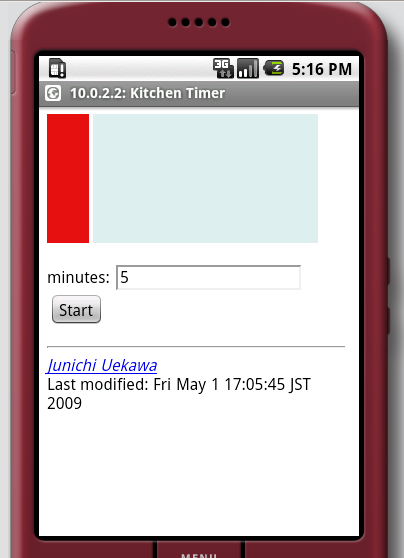
\includegraphics[width=0.3\hsize]{image200905/android-timer.png}

\subsection{Android$B$N4JC1$J%"%W%j%1!<%7%g%s$r:n@.$7$F5/F0$7$F$_$k(B}

$B$=$l$G$O!"(BAndroid $BMQ$N4JC1$J%"%W%j%1!<%7%g%s$r=q$$$F$_$^$7$g$&!#(B

\url{http://developer.android.com/guide/developing/eclipse-adt.html}
$B$K$7$?$,$C$FC8!9$H:n@.$7$^$9!#(B
$B$^$:!"(B
File$B$N(BNew Project $B$G(B Android $B$N$r%W%m%8%'%/%HA*Br$7$F:n@.$7$^$7$?!#(B
$B%?!<%2%C%H%S%k%I$O(B1.1$B$K$H$j$"$($:$7$m$H=q$$$F$"$j$^$9$,!"$h$/$o$+$i$J$$(B
$B$N$G!"<j85$N%U%!!<%`%&%'%"$N%P!<%8%g%s(B 1.5 $B$K$"$o$;$F$*$-$^$7$?!#(B

Run$B$N(BRun(Ctrl-F11)$B$G(BAndroid Application$B$rA*Br$9$k$H%(%_%e%l!<%?$r5/F0$7(B
$B$F%"%W%j%1!<%7%g%s$r<B9T$9$k$3$H$,$G$-$^$9!#(B
$B:G=i$K@8@.$5$l$?%=!<%9%3!<%I$N$^$^$N>uBV$@$H(B Hello World $B%"%W%j%1!<%7%g(B
$B%s$,5/F0$7$^$9!#(B

\subsection{Android$B$N4JC1$J%"%W%j%1!<%7%g%s$r=q$$$F$_$k(B}

$B%"%W%j%1!<%7%g%s$N:n@.$d%(%G%#%?$N5/F0$NItJ,$O$J$s$H$+$J$k$h$&$K$J$C$?$N(B
$B$G!"<!$O%A%e!<%H%j%"%k$rD/$a$F$_$^$9!#(B
Hello World$B$"$?$j$,$h$5$2$G$9!#(B

\url{http://developer.android.com/guide/tutorials/hello-world.html}

$B0lDL$jFI$s$G!"$H$j$"$($:%5%s%W%k$rD/$a$F$I$&$d$l$PJ8;zNs$rI=<($G$-$k$N$+(B
$B$r3NG'$7$?$N$G!"9%$-$JJ8;zNs$rI=<($9$k%"%W%j%1!<%7%g%s$r:n$C$F$_$^$9!#(B

Android $B$N(B top $B%3%^%s%I$G%W%m%;%9$N0lMw$r=PNO$G$-$k$N$G!"(B
$B%3%^%s%I$r<B9T$7$F$=$N=PNO$rI=<($9$k$@$1$N%"%W%j%1!<%7%g%s$r:n@.$7$F$_$^(B
$B$7$?!#(B
$BCf3K$r$J$9(Bsrc/jp.gr.netfort.dancer/TopView.java$B$O0J2<$N$h$&$K$J$j$^$7$?!#(B

\begin{commandline}
package jp.gr.netfort.dancer;

import android.app.Activity;
import android.os.Bundle;
import android.widget.TextView;
import java.io.*;

public class TopView extends Activity {
	/** Called when the activity is first created. */
	@Override
	public void onCreate(Bundle savedInstanceState) {
		super.onCreate(savedInstanceState);
		setContentView(R.layout.main);
		String [] command = { "top", "-n", "1"};
		String output = "";

		Runtime runtime = Runtime.getRuntime();
		Process process = null;
		try { 
			process = runtime.exec(command);
		} catch (Exception exception){
			System.exit(1);
		}
		BufferedReader reader = new BufferedReader(new InputStreamReader(process.getInputStream()));
		String line;
		try {
			while((line = reader.readLine()) != null) {
				output = output + line + "\n";
			}
		} catch (Exception exception) {
			System.exit(1);
		} finally {
			try {
				reader.close();
			} catch (Exception exception) {
				System.exit(1);
			}
		}
		TextView tv = new TextView(this);
		tv.setText(output);
		setContentView(tv);
	}
} 
\end{commandline}

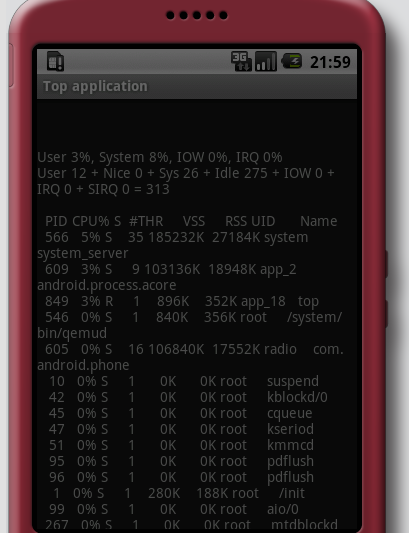
\includegraphics[width=0.3\hsize]{image200905/android-top.png}

\subsection{Android$B$N4JC1$J%"%W%j%1!<%7%g%s$r<B5!$G2TF/$5$;$F$_$k(B}

$B<B:]$K;H$&JXMx$J%"%W%j%1!<%7%g%s$r:n$C$F$_$^$7$g$&!#(B
$B%i%$%H%K%s%0%H!<%/$r<B;\$9$k:]$K$I$N%W%l%<%s%F!<%7%g%s$,5$$KF~$C$?$+$rI=(B
$BL@$9$k!"EjI<MQ$KMxMQ$9$k%\%?%s$G$b:n@.$7$^$7$g$&$+!#(B

\subsubsection{$B%(%U%'%/%HMQ$N%G!<%?(B}

$B$^$:!"$J$s$i$+$N8z2L2;$,I,MW$G$9!#(B
$B0JA0:n@.$7$?(Bding.wav $B$r$R$m$C$F$-$^$9!#(B
res/raw $B0J2<$K(B nautilus $B$+$i%I%i%C%0%"%s%I%I%m%C%W$G%3%T!<$7$^$9!#(B

$B$"$H!"%\%?%sIwL#$N2hA|$,I,MW$G$9!#(B
$BE,Ev$K(Bgimp$B$G3($r$+$$$F(B png $B%U%!%$%k$r:n@.$7$^$7$?!#(B

nautilus $B$+$i(B res/drawable $B0J2<$K(B png $B%U%!%$%k$r%I%i%C%0%"%s%I%I%m%C%W$G(B
$B%3%T!<$7$^$9!#(B

$B%U%!%$%kL>$+$i$=$N$^$^%j%=!<%9$NL>A0$r:n@.$9$k$?$a!"(B-$B$OMxMQ$G$-$J$$$h$&(B
$B$G$9!"(B \_ $B$OMxMQ$G$-$k$h$&$G$9!#:G=i(B he-up.png $B$r:n@.$7$h$&$H$7$F!"%(%i!<(B
$B$,=P$?$N$G(B he\_up.png $B$KJQ99$7$^$7$?!#(B

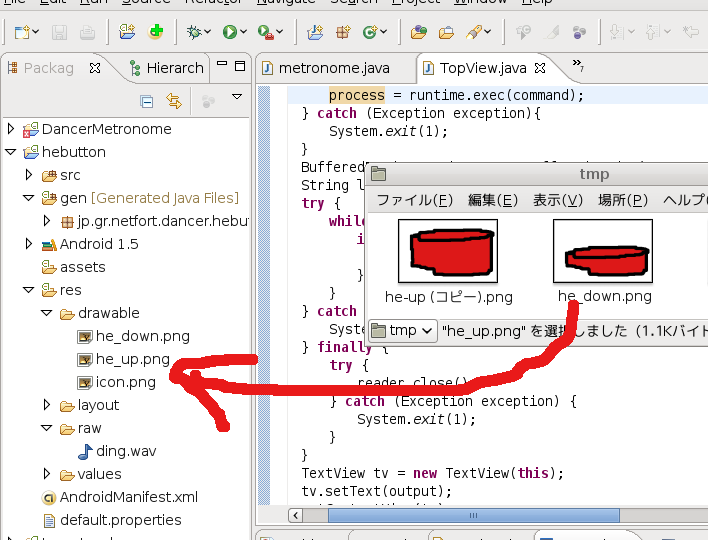
\includegraphics[width=0.5\hsize]{image200905/dragdrop.png}

\subsubsection{$B%l%$%"%&%H$N:n@.(B}

$B$*$b$`$m$K(B ImageButton $B$r:n@.$7$F!"(Bsrc$B$K2hA|%j%=!<%9$rDI2C$7$F$*$-$^$7$g(B
$B$&!#(B

\subsubsection{$B%/%j%C%/%"%/%7%g%s$N:n@.(B}

R.id.ImageButton01$B$KBP$7$F(B onClickListener$B$r:n@.$7!"%/%j%C%/$5$l$?=V4V$N(B
$BH?1~$r:n@.$7$^$7$g$&!#(B

$B2hA|$r%/%j%C%/$5$l$?>uBV$K@Z$jBX$($k$K$O(BImageButton$B$N(BsetImageResource()
$B$r8F$S=P$;$P$h$$$h$&$G$9!#(B

$B2;$r=P$9$K$O!"(BMediaPlayer $B$N%$%s%9%?%s%9$r:n@.$7!"(Bstart()$B$r8F$S=P$;$P$h(B
$B$$$h$&$G$9!#(B

$B0lDj;~4V7P2a$7$F$+$i85$N2hA|$KLa$9$K$O!"%"%i!<%`$r@_Dj$7$F%3!<%k%P%C%/$7(B
$B$F$b$i$($k$h$&$K$7$F!"%3!<%k%P%C%/$r8F$S=P$5$l$?$H$-$K=hM}$r$9$k$h$&$K$9(B
$B$l$P$h$$$h$&$G$9!#(B

\subsubsection{$B%5!<%PB&$N%"%/%7%g%s(B}

$B$=$l$G$O!"%/%j%C%/$5$l$?$H$-$K$I$&$$$&$3$H$r9T$&$N$+$N%"%/%7%g%s$r:n@.$7(B
$B$F$_$^$7$g$&!#(BHTTP$B%5!<%P$r=`Hw$7$^$9!#$3$&$$$&%$%m%b%N7O$N%5!<%P$r:n@.$9(B
$B$k$H$-$K$O(Bupaccho2 $B%5!<%P$r;H$&$3$H$,>e@n2H$N>o<1$J$N$G!"$=$l$rF'=1$7$^(B
$B$9!#(B($BM=Dj(B)

\subsection{$B$*$^$1(B:$B3+H/4D6-$KI,MW$J%a%b%j>CHq$O@a8:$G$-$k$N$+(B?}

$B<j85$N(BMacBook$B$K$O(B1GB$B$7$+%a%b%j$rEk:\$7$F$$$J$$$G$9!#(B
eclipse $B$O%G%U%)%k%H$N@_Dj$@$H5/F0$7$?=V4V$K(B1GB$B6a$/$N(B
$B2>A[%a%b%j$r>CHq$7!"B((BSwap$B$r;HMQ$7$F$7$^$&$H$$$&LdBj$,$"$j$^$7$?!#(B

\begin{commandline}
  PID USER      PR  NI  VIRT  RES  SHR S %CPU %MEM    TIME+  COMMAND            
17124 dancer    20   0  972m 302m  20m S    1 31.2   0:39.85 java
\end{commandline}

$B$H$j$"$($:!"%R%s%H$r5a$a$F(Bmaps$B$"$?$j$rD/$a$F$_$^$9!#(B
$B$=$l$J$j$K$?$/$5$s(Bmmap$B$7$F$$$^$9$,!"$=$l$@$1$G$O@bL@$G$-$J$$$h$&$J%a%b%j(B
$BNN0h$r3NJ]$7$F$$$^$9!#(B
\begin{commandline}
$ cat /proc/17124/status | grep Vm
VmPeak:	 1056748 kB
VmSize:	 1003316 kB
VmLck:	       0 kB
VmHWM:	  310740 kB
VmRSS:	  221616 kB
VmData:	  788504 kB
VmStk:	      84 kB
VmExe:	      36 kB
VmLib:	   38812 kB
VmPTE:	    1108 kB
$ cat /proc/17124/maps | grep rw | sort -rn -k5 
 .
\end{commandline}

$B$H$j$"$($:(BJava$B$N%"%W%j%1!<%7%g%s$N(BHeap$B$N;H$$J}$,$h$/$o$+$i$J$$$N$G!"(B
jconsole $B$G@\B3$7$FLdBj$r2r@O$7$^$9!#(B

$B%a%b%j%W!<%k$,$$$/$D$+$"$k$3$H$,$o$+$j$^$9!#(B

\begin{itemize}
 \item  Tenured Gen $B$,(B 60MB
 \item  Survivor 1MB
 \item  Code Cache $B$,(B 4MB
 \item  Perm Gen $B$,(B 70-90MB
 \item  Heap$B$O(B100MB(GC$B$7$?$i(B50MB$BDxEY(B)
\end{itemize}

eclipse.ini$B$,8=>u$3$&$J$C$F$$$k$N$G$9$,!"$3$l$r$*$=$k$*$=$k%A%e!<%K%s%0$7$F$_$^$9!#(B
\begin{commandline}
-showsplash
org.eclipse.platform
-framework
plugins/org.eclipse.osgi_3.4.2.R34x_v20080826-1230.jar
-vmargs
-Dosgi.requiredJavaVersion=1.5
-Xms40m
-Xmx256m
-XX:MaxPermSize=256m
\end{commandline}

$B5/F0;~$K3NJ]$7$?%R!<%W%a%b%j$NNN0h$r3+J|$7$F$$$J$$ItJ,$K$D$$$F$O!"(BGC$B$rIQ(B
$BHK$K9T$($P5/F0$O<c43CY$/$J$j$^$9$,$&$^$/$$$1$k$h$&$J5$$,$7$^$9!#(B
Xmx 128m$B$KJQ99$7$F$_$k$H!"<c43%a%b%j$N>CHq$,2<$,$j$^$7$?!#(B
$B$7$+$7$=$3$^$G7`E*$G$O$"$j$^$;$s$M!#(B
MaxPermSize$B$r(B64MB$B$K$9$k$H%(%i!<(B
\begin{commandline}
 Exception in thread "RMI TCP Connection(idle)" java.lang.OutOfMemoryError: PermGen space
\end{commandline}
$B$,H/@8$7$^$7$?!#(B
96MB$B$@$H%(%i!<$G$*$A$J$$$h$&$G$9!#(B

\begin{commandline}
  PID USER      PR  NI  VIRT  RES  SHR S %CPU %MEM    TIME+  $B%3%a%s%H(B
17124 dancer    20   0  972m 302m  20m S    1 31.2   0:39.85 java
19663 dancer    20   0  795m 296m  23m S    1 30.6   0:36.69 Heap 128MB$BHG(B
20266 dancer    20   0  661m 292m  22m S    1 30.1   0:41.62 MaxPermSize 96MB               
\end{commandline}

$B$,$s$P$C$F$_$?3d$K$O%a%b%j$,(B10MB$BDxEY$7$+@aLs$G$-$^$;$s$G$7$?!#%(%_%e%l!<(B
$B%?$b5/F0$7$F$$$k$H(B500MB$B$/$i$$(Bswap$B$K$$$C$F$7$^$&$N$G!"$D$i$$$G$9!#$7$+$b!"(B
$B%.%j%.%j$N%a%b%j@_Dj$K$7$F$$$?$H$3$m!"$$$m$$$m$HA`:n$7$F$$$k$H%a%b%j$,B-(B
$B$j$J$$$H$$$&%(%i!<$GMn$A$^$7$?!#$3$j$c%@%a$@!#%a%b%jGc$$$K$$$/$+$J!#(B

\begin{commandline}
-showsplash
org.eclipse.platform
-framework
plugins/org.eclipse.osgi_3.4.2.R34x_v20080826-1230.jar
-vmargs
-Dosgi.requiredJavaVersion=1.5
-Xms40m
-Xmx128m
-XX:MaxPermSize=96m
\end{commandline}

\subsection{$B;29MJ88%(B}

$BK\5-;v$N:n@.$K;29M$K$7$?J88%$G$9!#(B

\begin{itemize}
 \item \url{http://www.eclipse.org/}: eclipse
 \item \url{http://developer.android.com/}: Android $B$N%Z!<%8!"3+H/>pJs$,(B
       $B$^$H$^$C$F$$$k!#FC$K(B\url{http://developer.android.com/sdk/1.5_r1/index.html}: Android
       SDK 1.5$B$N%@%&%s%m!<%I%Z!<%8$+$i$?$I$k%Z!<%8$,=EMW!#(B
 \item
      \url{http://developer.android.com/guide/basics/what-is-android.html}: 
      SDK$B$N3+H/%^%K%e%"%k!#(B
      SDK $B$N(B\url{./android-sdk-linux_x86-1.5_r1/docs/}$B$KF1$8$b$N$,$"$k$N(B
      $B$G%*%U%i%$%s$G$b0B?4!#(B
      $B$?$@$7%*%s%i%$%s$N%I%-%e%a%s%H$OHyL/$JD{@5$,%"%C%W%G!<%H$5$lB3$1$F(B
      $B$$$k$h$&$J$N$G%M%C%H%o!<%/@\B3$,MxMQ$G$-$k%*%s%i%$%s$N>l9g$O$=$A$i(B
      $B$r;2>H$9$k$[$&$,$h$$$+$b$7$l$^$;$s!#(B
\end{itemize}

% ===============================================================
\dancersection{DDTSS$B3hMQ(B}{$B>e@n(B $B=c0l(B}
\index{DDTSS}
\index{DDTP}
% ===============================================================

\subsection{$B$O$8$a$K(B}

$B:G6a(B apt $B$N9q:]2=$b?J$_!"(BDebian archive $B$N(BDescription$B$NK]Lu$b%Q%C%1!<%8(B
$B$NG[I[$N;EAH$_$H0l=o$KG[I[$5$l$k$h$&$K$J$C$F$-$^$7$?!#(B
$B0lJ}!"K]Lu$rMQ0U$9$k%W%m%8%'%/%H(B(DDTP:Debian Description Translation
Project)$B$O$^$@Ia5Z$7$F$$$^$;$s!#(B
$B:#2s$O$=$N3hMQ$r;vA02]Bj$H$7$F!":#8e$I$&$d$C$F$&$^$/3hMQ$7$F$$$/$N$+$r9M(B
$B$($^$9!#(B

\subsection{Debian$B$N%Q%C%1!<%8@bL@J8$NK]Lu$NL\E*$H$O(B}

Debian Distribution$B$K$O?tK|$N%Q%C%1!<%8$,$"$j$^$9!#(B
$B%Q%C%1!<%8$N@bL@J8$O%$%s%9%H!<%k$9$k%=%U%H%&%'%"$rC5$9$N$K4sM?$9$kFbMF$G$"$kI,MW$,$"$j$^$9!#(B

$B8=:_!"$=$N@bL@J8$O$9$Y$F1Q(B
$B8l$GDs6!$5$l$F$$$^$9!#(B
$B$7$+$7!"1Q8l$G5-=R$5$l$F$$$k$H$=$b$=$b1Q8l$rM}2r$7$F$$$J$$$H$o$+$i$J$$It(B
$BJ,$,$"$j!"$7$+$b5;=QE*$J@lLgMQ8l$r$^$8$($?@bL@J8>O$OF|K\8l$r<g8@8l$H$9$k(B
$B%f!<%6$K$H$C$FM}2r$7$K$/$$>l9g$,$"$j$^$9!#(B

$B$=$b$=$b$N(BDescription$B$,K]Lu$KE,$9$k%l%Y%k$K;j$C$F$$$J$$!"F|K\8l$KLu$7$K$/(B
$B$$J8>O$G$"$l$P!"$b$H$NJ8=q$rD{@5$9$k$h$&$K0MMj$7$^$7$g$&!#(B

$B$^$?!"K]Lu$7$?(BDescription$B$,F|K\8l$H$7$FM}2r$7$K$/$$!"5;=QE*$JI=8=$,ITE,@Z$JI=8=$G$"$l$P!"$=$N(B
Description$B$OE,@Z$G$O$J$$$G$7$g$&!#(B

$B$^$?!"(BDebian$BA4BN$GI=5-$r$G$-$k$@$1E}0l$7$^$7$g$&!#F1$8FbMF$r@bL@$9$k$N$K(B
$BI=5-$N$f$l$,$"$k$H%Q%C%1!<%8$N@bL@J8$r$_$F$$$k$H$-$K$=$N:90[$KL\$,$$$C$F(B
$B$7$^$$$^$9!#(B

$B$=$NB>$K9MN8$9$kE@$O(B?

\subsection{DDTP}

DDTP $B$N@bL@$O(B Debian.org $B$N%Z!<%8$K$"$j$^$9(B: 
\url{http://www.debian.org/intl/l10n/ddtp.ja.html}$B!#(B
\url{http://www.debian.or.jp/community/translate/description-ja.html}
$B$J$I$H$"$o$;$FD/$a$F$/$@$5$$!#(B

$B%a!<%k%U%m%s%H%(%s%I$d!"%&%'%V%U%m%s%H%(%s%I$J$I$,$"$j$^$9!#(B

\subsection{DDTSS$B$H$O(B}

DDTP$B$N%U%m%s%H%(%s%I$N0l$D$,(BDDTSS$B$G$9!#(B
\url{http://ddtp.debian.net/ddtss/index.cgi/xx}
$B$KDs6!$5$l$F$$$^$9!#(B

\subsection{DDTSS$B3hMQ$N<j=g(B}

\subsubsection{$B%"%+%&%s%H$NEPO?(B}

$B%m%0%$%s2hLL(B\footnote{\url{https://ddtp.debian.net/ddtss/index.cgi/login}}$B$KHt$V$H!"(B
$B%"%+%&%s%H$r:n@.$9$k$?$a$N%j%s%/(B(Create$B!!(B
Login\footnote{\url{https://ddtp.debian.net/ddtss/index.cgi/createlogin}})
$B$,$"$k$N$G!"$=$3$+$i%"%+%&%s%HEPO?$7$^$9!#(B

$B%a!<%k$,FO$/$N$G!"$=$3$+$i%j%s%/$r%/%j%C%/$7$F%"%+%&%s%H$r%"%/%F%#%Y!<%H(B
$B$9$k$H!"%m%0%$%s2hLL$+$i%m%0%$%s$G$-$k$h$&$K$J$j$^$9!#(B

\subsubsection{$B%Q%C%1!<%8@bL@J8$NK]Lu:n@.(B}

\url{http://ddtp.debian.net/ddtss/index.cgi/ja}$B2hLL$G!"(B
Pending Translation $B$NMs$K$"$k%Q%C%1!<%8$rE,Ev$K%/%j%C%/$9$k$H!"%Q%C%1!<(B
$B%8@bL@J8$NJT=82hLL$,EP>l$7$^$9!#(B
$B0lIt$NJ8=q$,K]Lu$5$l$F$*$i$:(B\verb!<trans>!$B$H$J$C$F$$$?$j!"$^$C$?$/K]Lu$5(B
$B$l$F$$$J$+$C$?$j!"(B
$B>uBV$O$^$A$^$A$G$9!#(B

$B$3$N2hLL$GK]Lu$r:n@.$7$^$9!#(B

\subsubsection{$B%l%S%e!<$N<B;\(B}

\url{http://ddtp.debian.net/ddtss/index.cgi/ja}$B2hLL$G!"(B
Pending Review $B$NMs$K$"$k%Q%C%1!<%8$rE,Ev$K%/%j%C%/$9$k$H!"%Q%C%1!<%8@b(B
$BL@J8$N%l%S%e!<2hLL$,EP>l$7$^$9!#(B

$B%l%S%e!<$7$FJQ$JItJ,$,$"$l$PD{@5$7$^$7$g$&!#(B

\subsubsection{debian-doc$B%a!<%j%s%0%j%9%H$G$N%l%S%e!<<B;\(B}

debian-doc$B$H$$$&%a!<%j%s%0%j%9%H$G5DO@$H$+%l%S%e!<$O$*$3$J$&$_$?$$$G$9!#(B

\subsection{$B;29MJ88%(B}

$B0J2<$N%Z!<%8$b;29M$K$7$F$/$@$5$$!#(B

\begin{itemize}
 \item Debian $B%Q%C%1!<%8$N@bL@J8$rF|K\8l$GFI$_$?$$(B! $B!A(BDDTP $B$X$N$*M6$$!A(B 
       \url{http://www.debian.or.jp/community/translate/description-ja.html}
 \item $BIpF#7r;V$5$s$N(Bblog$B$N!X(BDebian$B%I%-%e%a%s%HK]Lu<jB3$-!Y(B:
       \url{http://kmuto.jp/d/index.cgi/debian/debian-doc-procedure.htm}
 \item $B>.NS576)$5$s$N(BDebian$BJY6/2q(B2006$BG/(B9$B7n;qNA!VK]Lu$X$NM6$$!W(B:
       \url{tokyodebian.alioth.debian.org/pdf/debianmeetingresume200609.pdf}
 \item debian-doc $B%a!<%j%s%0%j%9%H(B:
       $B<gMW$J5DO@$,9T$o$l$F$$$^$9!#<ALd$J$I$b!"$3$A$i$G!#(B
\end{itemize}

% from debianmeetingresume200812-kansai.tex
\dancersection{Debian $BJY6/2q$N;qNA$r:n@.$7$h$&(B}{$B;32<(B $BB:Li(B}

\subsection{$B%j%]%8%H%j$N%A%'%C%/%"%&%H(B}

\begin{commandline}
$ git clone git://git.debian.org/git/tokyodebian/monthly-report
\end{commandline}

\begin{commandline}
$ make -j4 # $B%(%i!<$,$G$^$9(B
$ cp -p git-pre-commit.sh .git/hooks/pre-commit
$ make -j4
\end{commandline}

\subsection{emacs whizzytex $B$N=`Hw(B}

\begin{commandline}
$ cd XXXXX
$ emacs 
\end{commandline}

whizzytex\footnote{$B%a%s%F%J$N>e@n$5$s$K$h$k;qNA$,(B
\url{http://www.netfort.gr.jp/~dancer/column/whizzytex.html.ja}$B$K$"$j$^(B
$B$9!#(B}$B$r5/F0$7$^$9!#(B
$B%W%j%S%e!<$,3+;O$9$k$H$$$&%a%j%C%H$@$1$G$J$/!"B(;~%3%s%Q%$%k%(%i!<$r8!=P(B
$B$G$-$k$N$,=EMW$G$9!#(B

\begin{commandline}
M-x whizzytex-mode 
\end{commandline}

$B%9%Z%k%A%'%C%/$b5/F0$7$^$7$g$&!#(B\footnote{iamerican $B$b$7$/$O(B ibritish $B%Q%C(B
$B%1!<%8$,I,MW$G$9!#(B}

\begin{commandline}
M-x flyspell-mode
\end{commandline}

\subsection{$B<+J,$N%;%/%7%g%s$rDI2C$9$k(B}
\label{sec:adddancersection}

$B$^$:<+J,$N%;%/%7%g%s$rDI2C$7$^$9!#(B

\begin{commandline}
 \dancersection{$B%;%/%7%g%sL>(B}{$BL>A0(B}
 \index{XXXX@YYYY}
 \label{XXXX@YYYY}

 % $BK\J8(B

\end{commandline}

\newpage

\subsection{$B%;%/%7%g%s$rDI2C(B}

\ref{sec:adddancersection}$B$G%;%/%7%g%s$rDI2C$7$^$7$?$N$G!"(B
$B<!$K%5%V%;%/%7%g%s$rDI2C$7$F$$$-$^$9!#I,MW$,$"$l$P!"%5%V%5%V%;%/%7%g%s$H(B
$BDI2C$7$F$$$-$^$9!#(B

\begin{commandline}

\subsection{xxxx} % $B%5%V%;%/%7%g%s(B($B>.@a(B)

\subsection{xxxx}

\subsubsection{xxxx} % $B%5%V%5%V%;%/%7%g%s(B($B>/!9@a(B)

\end{commandline}

\subsection{$BCm<a$rDI2C$9$k(B}

$B8=;~E@$G(B CDBS $B$r;HMQ$7$F$$$k%=!<%9%Q%C%1!<%8$O(B 1805 $B8D!"(B
$B%=!<%9%Q%C%1!<%8A4BN$N(B $\sim 16 \%$ $B$@$=$&$G$9(B
\footnote{$B$3$l!"@5$7$$$G$9$+$M(B? }$B!#(B

\begin{commandline}
$B8=;~E@$G(B CDBS $B$r;HMQ$7$F$$$k%=!<%9%Q%C%1!<%8$O(B 1805 $B8D!"(B
$B%=!<%9%Q%C%1!<%8A4BN$N(B $\sim 16 \%$ $B$@$=$&$G$9(B
\footnote{$B$3$l!"@5$7$$$G$9$+$M(B? }$B!#(B
\end{commandline}

\subsection{$B2hA|$rDI2C$9$k(B}
\label{sec:addpicture}

$B2hA|$rDI2C$9$kJ}K!$O$$$/$D$+J}K!$,$"$j$^$9$,!"(B
eps $B%U%!%$%k$@$H%U%!%$%k%5%$%:$,Bg$-$/$J$k$?$a!"(B
png $B$d(B jpg $B$J$I$KJQ49$r9T$J$C$?>e$GDI2C$7$?J}$,(B
$BNI$$$H;W$$$^$9!#(B

\begin{commandline}
M-! 
Shell command [~/monthly-report]$ cd image200808; ebb colinux_xlaunch_xdmcp.png
\end{commandline}

\begin{figure}[htbp]
 \begin{center}
  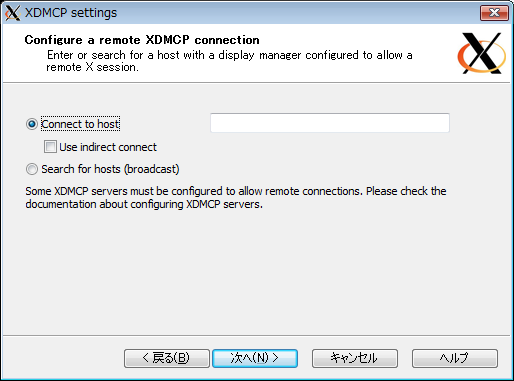
\includegraphics[width=100mm]{image200808/colinux_xlaunch_xdmcp.png}
 \end{center}
 \caption{XLaunch$B5/F0(B}
 \label{fig:colinux_xlaunch_xdmcp}
\end{figure}

\begin{commandline}
\subsection{$B2hA|$rDI2C$9$k(B}
\label{sec:addpicture}

\begin{figure}[htbp]
 \begin{center}
  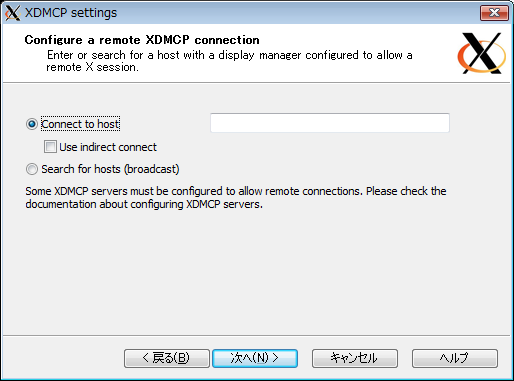
\includegraphics[width=100mm]{image200808/colinux_xlaunch_xdmcp.png}
 \end{center}
 \caption{XLaunch$B5/F0(B}
 \label{fig:olinux_xlaunch_xdmcp}
\end{figure}
\end{commandline}

\subsection{$B?^$dI=$r;2>H$9$k(B}

monthlyreport $B$G$O!"?^$dI=$r;2>H$9$k$N$KJXMx$J(B
\verb|\fgrep{}|$B$H(B\verb|\tbref{}|$B$,(B
$BDj5A$5$l$F$$$^$9!#(B

\ref{sec:addpicture}$B$G>R2p$7$?(B\fgref{fig:colinux_xlaunch_xdmcp}

\begin{commandline}
\ref{sec:addpicture}$B$G>R2p$7$?(B\fgref{fig:colinux_xlaunch_xdmcp}
\end{commandline}

\subsection{URL $B$rDI2C$7$F$_$k(B}

$B4X@>(B Debian $BJY6/2q$N>\:Y$K$D$$$F$O!"(B\url{http://wiki.debian.org/KansaiDebianMeeting}$B$K$"$j$^$9!#(B

\begin{commandline}
$B4X@>(B Debian $BJY6/2q$N>\:Y$K$D$$$F$O!"(B\url{http://wiki.debian.org/KansaiDebianMeeting}$B$K$"$j$^$9!#(B
\end{commandline}

\subsection{$BI=$r:n$C$F$_$k(B}

\LaTeX $B$GI=$r:n$k;v$b=PMh$^$9$,!";d$O(B OpenOffice Calc $B$G(B
$BI=$r:n@.$7!"(B\TeX $B$N%3!<%I$r@8@.$7$F$/$l$k(B
Calc2Latex\footnote{\url{http://calc2latex.sourceforge.net/indexj.html}}
$B$r;H$C$F$$$^$9!#(B

\subsection{$B2U>r=q$-(B}

$BMhG/EY$NM=Dj$O!"(B
\begin{itemize}
 \item Live Helper $B$N%O%s%:%*%s(B
 \item $BK]Lu%O%s%:%*%s(B\\
\dots{}
\end{itemize}

Debian $B$N%$%s%9%H!<%k$O!"(B
\begin{enumerate}
 \item $B8@8l@_Dj(B
 \item $B%-!<%\!<%I$NA*Br(B\\
\dots{}
\end{enumerate}

\begin{list}%
 {$\heartsuit$} %default label
 {Emacs $B$,9%$-$JM}M3(B} %formatting parameter
 \item $B%+%9%?%^%$%:2DG=(B
 \item $B;X$,3P$($F$$$k(B
 \item Emacs $B$NCf$@$1$G$[$H$s$I$N:n6H$,=PMh$k(B\\
\dots{}
\end{list}

\begin{commandline}
\begin{itemize}
 \item Live Helper $B$N%O%s%:%*%s(B
 \item $BK]Lu%O%s%:%*%s(B\\
\dots{}
\end{itemize}

Debian $B$N%$%s%9%H!<%k$O!"(B
\begin{enumerate}
 \item $B8@8l@_Dj(B
 \item $B%-!<%\!<%I$NA*Br(B\\
\dots{}
\end{enumerate}

\begin{list}%
 {$\heartsuit$} %default label
 {Emacs $B$,9%$-$JM}M3(B} %formatting parameter
 \item $B%+%9%?%^%$%:2DG=(B
 \item $B;X$,3P$($F$$$k(B
 \item Emacs $B$NCf$@$1$G$[$H$s$I$N:n6H$,=PMh$k(B\\
\dots{}
\end{list}
\end{commandline}

\subsection{$B$=$NB>$NCm0U;v9`(B}

\subsubsection{$B2~9T(B}

\LaTeX $B$G$O!"0lHLE*$J2~9T$N2r<a$H$O0[$J$j$^$9!#(B
$B6u$N9T$GCJMn$N6h@Z$j$HH=CG$7$^$9!#(B
$BCJMn$H$7$FH=CG$7$?$i!"9T$NF,$K(B1$BJ8;zJ,A43Q$N6uGr$,F~$j$^$9!#(B

\subsubsection{$B%3%^%s%I$N7k2L$K$D$$$F(B}

$B%3%^%s%I$N7k2L$J$I$r4JC1$K:\$;$i$l$k$h$&$K(B
kansaimonthlyreport.sty($B85$O!"(Bmonthlyreport.sty) $B$G$O!"(B
commandline $B$H8@$&JY6/2qMQ$KDj5A$5$l$F$*$j!"(B
commandline $B$rMxMQ$7$?J}$,4JC1$G$9!#(B

\subsubsection{$B%(%9%1!<%W$,I,MW$JJ8;zNs$N=PNOJ}K!(B}

\begin{itemize}
 \item \verb!\! verb $B$O8+$K$/$/$J$k$N$G:G=*E*<jCJ(B
 \item \~{}
 \item \^{}
 \item aaaa$<$aaaa $B$=$N$^$^$@$H(B:<
 \item aaaa$>$aaaa $B$=$N$^$^$@$H(B:>
 \item aaaa\#aaaa
 \item aaaa\%aaaa
 \item \_{}aaaa
\end{itemize}

\begin{itemize}
 \item {\tt /usr/share/iso-codes/iso\_3166.tab}
 \item /usr/share/iso-codes/iso\_{}3166.tab
\end{itemize}

\begin{commandline}
\begin{itemize}
 \item {\tt /usr/share/iso-codes/iso\_3166.tab}
 \item /usr/share/iso-codes/iso\_{}3166.tab
\end{itemize}
\end{commandline}

\subsubsection{$BA43Q1Q;z$J$I$N6X;_(B}

$B0lHLE*$KA43Q1Q;z!"H>3Q%+%J$N;HMQ$O;HMQ$7$^$;$s!#(B
$B$3$l$i$NGX7J$K$D$$$F$O!"8!:w$7$F$_$F2<$5$$!#(B

\dancersection{LaTeX beamer $B$G%W%l%<%s%F!<%7%g%s(B}{$BBg1:(B $B??(B}

\subsection{$B$O$8$a$K(B}

\begin{itemize}
\item Debian$BJY6/2q$J$I$G$O!"9V;U$r$9$k:]$K%W%l%<%sMQ$N;qNA$,I,MW$K$J$k!#(B
\item $B$I$&$d$C$F:n$k$+!#(B
  \begin{itemize}
  \item MS Power Point $B$d(B Openoffice.org $B$N(B Impress$B!#(B
  \item Magic Point$B!#(B
  \item HTML $B$H%V%i%&%6!#(B
  \item $B%F%-%9%H%U%!%$%k$H(B less$B!#(B
  \item \LaTeX{}$B$G:n$k!#(B
  \end{itemize}
\end{itemize}


\subsection{LaTeX beamer}

\subsubsection{$BFCD'(B}

\begin{itemize}
\item \LaTeX{}$B$,%Y!<%9!#(B
  \begin{itemize}
  \item $BFCJL$J$3$H$O$7$F$$$J$$$N$G!"(B\LaTeX{}$B$5$(J,$+$l$P;H$($k!#(B
  \end{itemize}
\item $B:G?7HG$O(B 2007$BG/(B3$B7n%j%j!<%9$N(B 3.07$B!#(B
\item $BK-IY$J%F!<%^!"K-IY$J%5%s%W%k$,MQ0U$5$l$F$$$k!#(B
\item $B4JC1$J%"%K%a!<%7%g%s$/$i$$$O$G$-$k!#(B
\item \verb|\section|$B!"(B\verb|\subsection| $B$rIaDL$K;H$($k!#(B
\item $B3+H/$,@9$s!#(B
  \begin{itemize}
  \item $B%^%K%e%"%k$OA4(B 224$B%Z!<%8!#(B
  \end{itemize}
\end{itemize}

\newpage

\subsubsection{$B%$%s%9%H!<%k(B}


\begin{itemize}
\item \LaTeX{}$B0l<0$,I,MW!#(BDebian $B$J$i(B texlive $B$r%$%s%9%H!<%k$9$k!#(B
\item latex-beamer $B$N%$%s%9%H!<%k(B
  \begin{itemize}
  \item \url{http://latex-beamer.sourceforge.net/} $B$+$i%@%&%s%m!<%I!#(B
  \item latex-beamer $B0J30$K$b(B pgf $B$H(B xcolor $B$bI,MW!#(B
  \item Debian $B$@$C$?$i!"(B\texttt{\# apt-get install latex-beamer}
  \item $B<jF0$G%$%s%9%H!<%k$9$k>l9g$O!"(B
    \texttt{/usr/share/texmf} $B$J$I$K(B texmf $B$H$$$&(B
    $B%G%#%l%/%H%j$,$"$k$N$G!"(B
    texmf/tex/latex/beamer $B$J$I$N%5%V%G%#%l%/%H%j$r:n$C$F(B
    $B$=$3$K%9%?%$%k%U%!%$%k$r%3%T!<!#(B
  \end{itemize}
\end{itemize}


\subsubsection{$B4pK\E*$J;H$$J}(B}

\begin{itemize}
\item $B%/%i%9%U%!%$%k$H$7$F(B beamer.cls $B$r;H$&!#(B
\begin{commandline}
\documentclass{beamer}
\end{commandline}
\item $B;H$&%F!<%^$r7h$a$k!#(B
\begin{commandline}
\usetheme{Boadilla}
\end{commandline}
\item $B%?%$%H%k!":n<T!"F|IU$N@_Dj!#(B

\begin{commandline}
\title{LaTeX beamer $B$G%W%l%<%s%F!<%7%g%s(B}
\author{$BBg1:!w(BDebian.org}
\date{2008$BG/(B12$B7n(B14$BF|(B($BF|(B)}
\end{commandline}

\item $B%9%i%$%I0lKg0lKg$O%U%l!<%`$H8F$P$l$k!#(B
  $B%U%l!<%`$O(B\verb|\begin{frame}|$B$H(B\verb|\end{frame}|$B$G0O$`!#(B
\item $B%?%$%H%k%Z!<%8$r:n$k!#(B

\begin{commandline}
\begin{frame}
\titlepage{}
\end{frame}
\end{commandline}

\item $BI,MW$J$iL\<!$N%Z!<%8$r:n$k!#(B
  \begin{itemize}
  \item $BK\J8Cf$G(B \verb|\section{}| $B$J$I$r;H$($P<+F0E*$KL\<!$,:n$i$l$k!#(B
    $B%F!<%^$K$b$h$k$,!"%9%i%$%I$NCf$K%;%/%7%g%sL>$,I=<($5$l$k!#(B
  \end{itemize}

\begin{commandline}
\begin{frame}
\frametitle{$BL\<!(B}
\tableofcontents{}
\end{frame}
\end{commandline}

\item $BE,59%;%/%7%g%s$KJ,$1$k!#(B
\item $B%W%l%<%s%F!<%7%g%s$OJ#?t$N%U%l!<%`$G$G$-$F$$$k!#(B
\item \verb|\frametitle{}|$B$,$=$N%Z!<%8$N%?%$%H%k!#(B

\begin{commandline}
\begin{frame}
\frametitle{$B$O$8$a$K(B}
\begin{itemize}
\item Debian$BJY6/2q$J$I$G$O!"9V;U$r$9$k:]$K%W%l%<%sMQ$N;qNA$,I,MW$K$J$k!#(B
  ....
\end{itemize}
\end{frame}
\end{commandline}

\end{itemize}


\subsubsection{$B%U%l!<%`$H%9%i%$%I(B}

\begin{itemize}
\item $B%U%l!<%`$OJ#?t$N%9%i%$%I$+$i$G$-$F$$$k!#(B
\item \verb|\pause{}|$B$r;H$&$H0l$D$N%U%l!<%`$rJ#?t$KJ,3d$G$-$k!#(B

\begin{commandline}
\begin{frame}
\frametitle{$B$O$8$a$K(B}
\begin{itemize}
\item Debian$BJY6/2q$J$I$G$O!"9V;U$r$9$k:]$K%W%l%<%sMQ$N;qNA$,I,MW$K$J$k!#(B
\pause{}
\item $B$I$&$d$C$F:n$k$+!#(B
    ....
\end{itemize}
\end{frame}
\end{commandline}

\item $BFCDj$N%9%i%$%I$@$1$G%3%^%s%I$rM-8z$K$G$-$k!#(B
\item \LaTeX{}$B$N%3%^%s%I$N8e$K(B \verb|< >| $B$rIU$1$k!#(B

\begin{commandline}
\begin{itemize}
\item \textbf{$B$3$N9T$O>o$KB@;z$G$9!#(B}
\item \textbf<2>{$B$3$N9T$O(B2$BKgL\$N%9%i%$%I$G$N$_B@;z$G$9!#(B}
\item \textbf<3>{$B$3$N9T$O(B3$BKgL\$N%9%i%$%I$G$N$_B@;z$G$9!#(B}
\end{itemize}
\end{commandline}

\end{itemize}


\subsubsection{$B4JC1$J%"%K%a!<%7%g%s(B}


\begin{itemize}
\item $B$4$/4JC1$J%"%K%a!<%7%g%s$,;H$($k!#(B
\item \verb|\animate| $B$H(B \verb|\animatevalue| $B$r;H$&!#(B

\begin{commandline}
\newcount\opaqueness
\begin{frame}
  ....
\animatevalue<1-10>{\opaqueness}{100}{0}
\begin{colormixin}
{\the\opaqueness!averagebackgroundcolor}
$B$3$NJ8;zNs$O%U%'!<%I%"%&%H$7$^$9!#(B
\end{colormixin}
\end{frame}
\end{commandline}

\end{itemize}


\subsubsection{$B2hA|$N<h$j9~$_(B}

\begin{itemize}
\item \LaTeX{}$B$J$N$GIaDL$K2hA|$b<h$j9~$a$k!#(B
\item $BNc$($P(B Debian $B$N(B logo$B!#(B\texttt{openlogo.eps}
\item \texttt{graphicx.sty} $B$r;H$&!#(B

\begin{commandline}
\includegraphics[height=3cm,keepaspectratio,clip]{openlogo.eps}
\end{commandline}

\end{itemize}

\subsection{$B%W%l%<%s$NJ}K!(B}

\begin{itemize}
\item dvi $B%U%!%$%k$r:n$C$F!"(Bxdvi $B$G%W%l%S%e!<$9$k$H2hA|$,I=<($5$l$J$$$,!"(B
  $B:n@.ESCf$N%W%l%S%e!<$K$O==J,!#(B
\item $B%W%l%<%s$N:]$K$O!"(BPostscript $B$+(B PDF $B$KJQ49$9$k!#(B
\item Postscript $B$K$9$k>l9g$O!"(Bdvips $B$r;H$&!#(B
  \begin{itemize}
  \item \texttt{beamer.cls}$B$K%*%W%7%g%s(B\texttt{dvips}$B$rIU$1$k!#(B
    \verb|\documentclass[dvips]{beamer}|
  \item pspresent $B$r;H$C$FI=<(!#(B
    \url{http://www.cse.unsw.edu.au/~matthewc/pspresent/}
  \end{itemize}
\item PDF $B$K$9$k>l9g$O!"(Bdvipdfmx $B$+!"(B
  Postscript $B$KJQ49$7$F$+$i(B Ghostscript (ps2pdf) $B$r;H$&!#(B
  \begin{itemize}
  \item dvipdfmx $B$r;H$&$?$a$K$O!"(B\texttt{beamer.cls}$B$K(B
    $B%*%W%7%g%s(B\texttt{dvipdfm}$B$rIU$1$k!#(B
  \item Acrobat Reader $B$r;H$C$FI=<(!#(Bhyperlink $B$N5!G=$b;H$($k!#(B
  \end{itemize}
\item $BG[I[MQ$N;qNA$G$O%"%K%a!<%7%g%s$J$I$OL58z$K$9$k!#(B
  $B%"%K%a!<%7%g%s$OJ#?t%Z!<%8$H$7$F07$o$l$k$N$G!"$=$l$r(B1$B%Z!<%8$K$9$k!#(B
  \begin{itemize}
  \item \texttt{beamer.cls}$B$K%*%W%7%g%s(B\texttt{handout}$B$rIU$1$k!#(B
  \end{itemize}
\item Postscript $B$+$i0u:~$9$k>l9g$O!"(Bpsutils $B$K4^$^$l$k(B
  psnup $B$G(B 1$B%Z!<%8$KJ#?t$N%U%l!<%`$rF~$l$F0u:~!#(B
  \begin{itemize}
  \item psutils
    \url{http://www.dcs.ed.ac.uk/home/ajcd/psutils/}
  \end{itemize}
\end{itemize}


\subsubsection{$B=*$o$j$K(B}


\begin{itemize}
\item \LaTeX{}$B$N;H$$J}$5$(J,$+$C$F$$$l$P(B
  latex-beamer $B$O4JC1$K;H$($^$9!#(B
\item \LaTeX{}$B>e$NB>$N%W%l%<%s%F!<%7%g%s%9%?%$%k$h$j$b(B
  $BGI<j$J%9%i%$%I$r:n$l$^$9!#(B
\item $B$<$R!"(Blatex-beamer $B$r;H$C$F(B Debian $BJY6/2q$G9V;U$r$7$^$7$g$&!#(B
\end{itemize}

% from debianmeetingresume200904-kansai.tex

\dancersection{$B%Q%C%1!<%8$N0MB8@-$r2r$/!'(BEDOS $B$+$i(B Mancoosi $B$^$G(B}{Ralf Treinen}


$BCm(B) Ralf Treinen $B$5$s$NH/I=MQ%9%i%$%I$r!"4JC1$+$DE,Ev$K>6Lu$7$^$7$?!#(B
%$B1Q8l$,6l<j$JJ}$O!"H/I=A0$K$6$C$HFI$s$GFbMF$rGD0.$7$F$*$$$F$/$@$5$$!#(B

$BLu$N4V0c$$$J$I!"6l>p$OARI_$^$G!#(B

\subsection{Mancoosi $B%W%m%8%'%/%H(B}

\begin{itemize}
\item $B%h!<%m%C%Q$K$*$1$k8&5f%W%m%8%'%/%H(B
\item $B4|4V!'(B2008/2 $B"*(B 2011/1
\item EDOS $B%W%m%8%'%/%H(B (2004/1 $B"*(B 2007/6) $B$N8e7Q(B
\end{itemize}


\subsection{EDOS $B$H(B Mancoosi $B$NL\E*(B}

\begin{itemize}
\item $B%3%s%T%e!<%?%5%$%(%s%9$N8&5f@.2L$r%U%j!<(B/$B%*!<%W%s%=!<%9%=%U%H%&%'%"(B (F/OSS) $B%G%#%9%H%j%S%e!<%7%g%s$K1~MQ!'(B

\begin{itemize}
\item $B7A<0<jK!!'O@M}$K4p$/%D!<%k$H<jK!(B from Verification
\item $B%D!<%k(B from $B%=%U%H%&%'%"9)3X(B
\end{itemize}
\item F/OSS $B%G%#%9%H%j%S%e!<%7%g%s$H!"2J3XE*8&5f$K$*$$$F!"E~C#?e=`$r8~>e$5$;$k$N$,L\E*(B
\end{itemize}


\subsection{$B$J$<2J3X8&5f<T$,(B F/OSS $B$K6=L#$r$b$D$N$+!)(B}

F/OSS $B%$%s%U%i%9%H%i%/%A%c$,FC$K6=L#?<$$$N$O!'(B

\begin{itemize}
\item $BCf?4$H$J$k@_7W<T$,$$$J$$(B
\item $B3+H/$,B.$/!"J,;6$5$l$F$$$k(B
\item $B%Q%C%1!<%8$NAj8_0MB8$,6/$$(B
\item $B5pBg$J%3!<%I%Y!<%9(B
\item $BF1;~$KJ#?t$N(B CPU $B%"!<%-%F%/%A%c$K%Q%C%1!<%8$rDs6!(B
\item $BJ#?t$N(B OS $B$KBP$7$FF1;~$K%Q%C%1!<%8$rDs6!(B
\end{itemize}


\subsection{$B$J$<(B F/OSS $B$,2J3X$N8&5f@.2L$K6=L#$r$b$D$N$+!)(B}

F/OSS $B$K$*$1$kIJ<AJ]>Z$N8=>u$O!'(B

\begin{itemize}
\item $B%3%s%Q%$%k$H%$%s%9%H!<%k$N(B ($B;~$K$O<+F02=$5$l$?(B) $B%F%9%H(B
\item $B%F%9%H%1!<%9$N<+F0@8@.$O$J$5$l$J$$(B
\item $B<+F08!>Z%D!<%k$O;H$o$l$F$$$J$$(B
\item $B8DJL$N%Q%C%1!<%8$H!"%G%#%9%H%j%S%e!<%7%g%sA4BN$K$D$$$F!"IJ<AJ]>Z$N$?$a$N<+F02=$5$l$?%D!<%k$,I,MW$KGw$i$l$F$$$k(B
\end{itemize}


\subsection{$B%Q%C%1!<%8$N0MB84X78$K$*$1$k(B EDOS workpackage}

$B>GE@!'%j%j!<%94IM}<T$N4QE@$K$h$k%G%#%9%H%j%S%e!<%7%g%s$N0l4S@-(B

$B<ALd!'5,Dj$N%j%]%8%H%j$K$"$k%Q%C%1!<%8$7$+;H$($J$$>l9g$K!"%f!<%6$,A*Br$7$?%Q%C%1!<%8$O%$%s%9%H!<%k2DG=$@$m$&$+!)(B

$B%j%j!<%94IM}<T$dIJ<AJ]>Z%A!<%`$,!"LdBj$N$"$k!"$b$7$/$OL5MQ$J%Q%C%1!<%8$r8+$D$1$k=u$1$K$J$k<ALd(B



\subsection{$B%Q%C%1!<%8$N%$%s%9%H!<%i%S%j%F%#(B as SAT ($BL?BjO@M}$N=<B-2DG=@-H=DjLdBj(B)}

$B%Q%C%1!<%8$N4X78$K$D$$$F!"L?BjO@M}$K4p$$$F?t3XE*$J%b%G%k$r:n$k$3$H$+$i;O$a$?!#(B

\begin{itemize}
\item $B3F%Q%C%1!<%8(B p ($B%P!<%8%g%s$O(B v) $B$O!"%V!<%kJQ?t(B Pv (Pv $B$G$"$l$P%Q%C%1!<%8$O%$%s%9%H!<%k2DG=!#$=$&$G$J$1$l$PIT2DG=(B) $B$H$7$F2r<a$5$l$k(B
\item $B0MB84X78$O!"$=$l$>$lO":?$H$7$F2r<a$5$l$k!#Nc!'(Baterm $B"*(Blibc6 \^{} (libice6 v xlibs) \^{} \dots{}
\item $B%Q%C%1!<%8(B a $B$H(B b $B$G$N>WFM$O!"8x<0(B !(a \^{} b) $B$H$7$F2r<a$5$l$k(B
\end{itemize}

$BDjM}!'(B

$B$"$k%Q%C%1!<%8(B p $B$N%P!<%8%g%s(B v $B$O!"(BPv $B$r??$H$9$k??56CM$,B8:_$7!"%j%]%8%H%j$N5-9f2=$rK~B-$9$l$P!"!V%$%s%9%H!<%k2DG=!W$G$"$k(B


\subsection{$B%Q%C%1!<%8%$%s%9%H!<%k$NMF0W$5(B as SAT $B!](B $BNc(B}


$BJ?6QE*$J<0$O(B 400 $B$NDj?t$r;}$D!#(BKDE $B$N%$%s%9%H!<%k$G$O(B 32000


\subsection{EDOS $B%D!<%k%A%'%$%s(B}

EDOS $B$rDL$8$F$$$/$D$+$N%D!<%k$,3+H/$5$l$?(B (OCaml $B$G(B 110000 $B9T$N%3!<%I(B)

\begin{description}
\item[edos-debcheck] \mbox{}

$B%Q%C%1!<%8$N%$%s%9%H!<%i%S%j%F%#$r%A%'%C%/$9$k%3%^%s%I%i%$%s%D!<%k(B
\item[pkglab] \mbox{}

$B%$%s%?%i%/%F%#%V$J%3%s%=!<%k4D6-$G!"%j%]%8%H%j$N8!::MQ(B
\item[ceve] \mbox{}

$B%Q%C%1!<%8%j%9%H$NJ#?t%U%)!<%^%C%H$r%Q!<%9(B/$BJQ49$9$k(B
\item[tart] \mbox{}

$B%j%]%8%H%j$rJ,3d(B ($B%a%G%#%"$J$I(B) $B$9$k!#$3$N;~!"(Bi $BHVL\$N%a%G%#%"$K4^$^$l$F$$$k%Q%C%1!<%8$O!"(Bi $BHVL\$^$G$N%a%G%#%"$r;H$($P%$%s%9%H!<%k2DG=$H$J$k(B
\end{description}

$B$$$/$D$+$r>\:Y$K8+$F$_$h$&!D!D(B


\subsection{edos-debcheck}

\begin{itemize}
\item edos-debcheck $B$O(B APT $B%Q%C%1!<%8%j%9%H(B (/var/lib/apt/lists/* $B$J$I(B) $B$r$b$H$K!"$"$k(B/$B$$$/$D$+$N(B/$BA4$F$N%Q%C%1!<%8$,%$%s%9%H!<%k2DG=$+$I$&$+$r%A%'%C%/$9$k(B
\end{itemize}

$B%+%9%?%^%$%:$5$l$?(B SAT $B2r7h4o$,%Y!<%9$K$J$C$F$$$F!"$H$F$b9bB.!'(Btesting/amd64 $B$N(B main $B$K$"$kA4%Q%C%1!<%8$N%$%s%9%H!<%i%S%j%F%#$N%A%'%C%/$K$+$+$k;~4V$O!"%(%s%H%j!<%l%Y%k$N%^%7%s>e$G(B 5 $BIC!#(B

\begin{description}
\item[$BBg$-$J@.8yNc(B] \mbox{}

emdebian $B$G$O%Q%C%1!<%8$N%"%C%W%m!<%IA0$K(B edos-debcheck $B$r;H$C$F!"2u$l$?%Q%C%1!<%8$r%"!<%+%$%V$K%"%C%W%m!<%I$7$J$$$h$&$K$7$F$$$k(B
\end{description}

Debian $B$N%Q%C%1!<%8L>!'(Bedos-debcheck, edos-rpmcheck


\subsection{pkglab}

- pkglab $B$O%$%s%?%i%/%F%#%V$J!"%3%s%=!<%k%Y!<%9$N4D6-$G!"%Q%C%1!<%8%Y!<%9$N%=%U%H%&%'%"%G%#%9%H%j%S%e!<%7%g%s$N%j%]%8%H%j$rD4::$9$k$b$N(B

$B5!G=!'(B

\begin{itemize}
\item $B8=:_$H2a5n$N%Q%C%1!<%8%j%9%H$rFI$_9~$`(B
\item $B%Q%C%1!<%8$N%$%s%9%H!<%i%S%j%F%#$r%A%'%C%/(B (edos-debcheck $B$G(B)
\item $B4X?t7?$N%/%(%j8@8l(B (map, filter, fold, \dots{})
\item $B%j%]%8%H%j$,$I$N$h$&$JJQA+$r7P$FH/E8$7$F$-$F$$$k$+$rD4$Y$k(B (edos-debcheck $BC1BN$G$OIT2DG=(B)
\end{itemize}

Debian $B$N%Q%C%1!<%8L>!'(Bdose2 ($B4pK\$N%i%$%V%i%j(B), ceve ($B%Q%C%1!<%8%j%9%H$N%Q!<%5(B/$B%3%s%P!<%?(B), pkglab ($B%$%s%?%i%/%F%#%V4D6-(B), edos-debcheck (debian $B8~$1$N%$%s%9%H!<%i%S%j%F%#%A%'%C%+(B), edos-rpmcheck (RPM $B8~$1$N%$%s%9%H!<%i%S%j%F%#%A%'%C%+(B)


\subsection{Debian $B$G!"%$%s%9%H!<%k$G$-$J$$%Q%C%1!<%8$r8+$D$1$k(B}

Debian, Skilelinux, Debian GNU/kFreeBSD $B$K$*$$$F!"KhF|(B edos-debcheck $B$r;H$C$F%$%s%9%H!<%kIT2DG=$J%Q%C%1!<%8$r%b%K%?!<$7$F$$$k!'(B

\url{http://edos.debian.net/edos-debcheck}

$B%$%s%9%H!<%k$G$-$J$$%Q%C%1!<%8$NIQ=P%1!<%9!'(B

\begin{enumerate}
\item autobuilder $B$NDI?o(B ($BNc$($P!"(Barch:all $B$N%Q%C%1!<%8$,(B arch:any $B$N%Q%C%1!<%8$HF1;~$K%"%C%W%m!<%I$5$l!"(Bautobuilder $B$,CY1d$7$F$$$k(B)$B!'DL>o$N0l2a@-$N%$%s%9%H!<%kIT2D>uBV(B
\item a $B$,(B b $B$K0MB8$7$F$*$j!"A4%"!<%-%F%/%A%c$K(B b $B$,$J$$!'(Bb $B$N%S%k%I$KLdBj$,$"$C$?$j!"(Ba $B$K$*$$$F!"$H$C$F$b$*$*$i$+$J%"!<%-%F%/%A%c;XDj$,$J$5$l$F$$$k(B ($B87L)$K$9$Y$-(B)

\begin{itemize}
\item $B>e5-$NFC<l$JNc!'(Ba $B$O(B arch:all$B!#:G6a$N(BInstall-To $B%U%#!<%k%I$rDI2C$9$kDs0F$O$3$l$KBP=h$9$k$b$N(B (\#436733)
\end{itemize}
\item $B?<9o$J%Q%C%1!<%8$N%P%0$G!"<B:]$K=$@5$9$kI,MW$,$"$k(B :-)
\end{enumerate}


\subsection{Debian $B$G!"@k8@$5$l$F$$$J$$>WFM$r8+$D$1$k(B}

$B%f!<%6$K$3$&$$$C$?%(%i!<$r8+$;$kA0$K<h$j=|$/!#(B

\begin{enumerate}
\item $B6rD>$K!'%Q%C%1!<%8A4It(B (200,000,000) $B$rF1;~$K%$%s%9%H!<%k$7$F$_$k!D!D$=$s$J%P%+$J(B!
\item $B>/$J$/$H$b(B 1 $B%U%!%$%k$r6&M-$7$F$$$k%Z%"$N$_9MN8(B (Contents $B$r;H$($P4JC1(B)$B!'(B867 $B%Z%"(B (2008/4/16 $B$N(B amd64/sid)
\item $B0MB8@-$N$&$($GF1;~%$%s%9%H!<%k2DG=$J%Z%"$K9J$k(B (pkglab $B$r;H$($P4JC1(B)$B!'(B102 $B%Z%"(B
\item diversion $B$K$h$C$F8m8!CN$5$l$F$$$k$+$b!'%Z%"$G$N%$%s%9%H!<%k$r(B chroot $B4D6-$G%F%9%H!'(B27 $B$N%P%0$b$A%Q%C%1!<%8%Z%"$,8!=P$5$l$?(B
\end{enumerate}

$B%l%]!<%H!'(B\url{http://edos.debian.net/missing-conflicts/}

BTS:$B%f!<%6(B \verb|treinen@debian.org|$B!"%?%0(B edos-file-overwrite


\subsection{Mancoosi $B%W%m%8%'%/%H(B}

$B%"%C%W%0%l!<%ILdBj(B = $B%$%s%9%H!<%k$5$l$?%Q%C%1!<%8$N%m!<%+%k$J%9%F!<%?%9$rJQ99$9$k$h$&%a%?%$%s%9%H!<%i$,MW5a$9$k$3$H$GH/@8$9$kLdBj!#(B

$B%"%C%W%0%l!<%ILdBj$N2r7h$O!"$$$/$D$+$NM}M3$G<:GT$7F@$k!'(B

\begin{itemize}
\item $B8F$S=P$7%(%i!<!"0MB8@-2r7h!"%Q%C%1!<%8<u?.!"%Q%C%1!<%8E83+!"%a%s%F%J%9%/%j%W%H$N<B9T!"!D!D(B
\end{itemize}

Mancoosi $B$O(B 2 $B$D$NB&LL$+$i%"%C%W%0%l!<%ILdBj$K<h$jAH$b$&$H$7$F$$$k!'(B

\begin{description}
\item[$B%m!<%k%P%C%/$N%5%]!<%H(B] \mbox{}

$BA[Dj30$N%(%i!<(B ($B%a%s%F%J%9%/%j%W%H$J$I(B) $B$,$"$C$?>l9g!";v8e$N%j%+%P%j$,M#0l$N2r7h:v(B
\item[$B0MB8@-2r7h(B] \mbox{}

$B%a%?%$%s%9%H!<%i$,:G?7$N?e=`$rK~$?$7$F$$$J$$(B ($BNc$($P!"IT40A4@-!'(Bwhen there is one$B!"2r7hK!$r8+$D$1$k$3$H$,$G$-$J$$(B)$B!'2f!9$,$&$^$/$d$i$M$P!*(B
\end{description}


\subsection{$B0MB8@-$N2r7h$KI,MW$J$b$N(B}

\begin{description}
\item[$B40A4@-(B] \mbox{}

$B%"%C%W%0%l!<%ILdBj$X$N2r7hK!$,B8:_$9$k$J$i!"%a%?%$%s%9%H!<%i$O$=$l$rH/8+$G$-$J$/$F$O$J$i$J$$(B
\item[$B:GE,@-(B] \mbox{}

$BF1Ey$N0[$J$kJ#?t$N2r7hK!$r6hJL$9$k$?$a!":GE,2=$N4p=`$r;XDj$G$-$kI,MW$,$"$k!#Nc$($P!'(B
\end{description}

\begin{itemize}
\item $B%@%&%s%m!<%I%5%$%:$r:G>.2=(B
\item $B;HMQ$9$k%G%#%9%/%9%Z!<%9$r:G>.2=(B
\item J. Random DD (DD $B$NC/$+(B) $B$,%a%s%F$7$F$$$k%Q%C%1!<%8$N%V%i%C%/%j%9%H(B
\item $B$J$I$J$I(B
\end{itemize}

\begin{description}
\item[$B8zN((B] \mbox{}

$B0MB8@-$N2r7h$O!"2DG=$J8B$j9bB.$G$J$/$F$O$J$i$J$$(B
\end{description}

\subsection{$B0MB8@-2r7hK!$N(B competition}

$B2f!9$O!"0MB8@-2r7h$K$*$1$kKbK!$N6d$NCF4]$H$J$k%"%k%4%j%:%`$rC5$=$&$H$7$F$$$k$o$1$G$O$b$A$m$s$J$$$,!"0MB8@-2r7h$N(B competition $B1?1D$K$D$J$,$k=u$1$H$J$k$3$H$,$G$-$k(B

\begin{itemize}
\item popcon $B$N$h$&$K<}=8$7$?8=<B$K$*$1$k%"%C%W%0%l!<%ILdBj(B ($B%a%?%$%s%9%H!<%i$,;}$D%*%W%H%$%s$N%G!<%?<}=8%W%i%0%$%s(B)
\item $BMM!9$J>Z@W!'J?0W$JJ,@O(B ($B%9%T!<%I(B)$B!":GE,2=$7$?J,@O(B ($B$h$j$h$$2rK!(B)$B!"!D!D(B
\item $B3+H/<T$H8&5f<T$,!"FH<+%"%k%4%j%:%`$NFH<+<BAu$rDs<($9$k$3$H$,$G$-$k(B
\item $B>!<T$O9,1?$H1I8w$r%2%C%H(B
\end{itemize}

SAT $B2r7h<+BN$N$h$&$J4XO"J,Ln$K$*$$$F!"F1MM$N(B competition $B$,5;=Q?e=`$r:G?7$K2!$7$"$2$k$N$KBg$$$K4sM?$7$F$$$^$9!#$J$<$3$NJ,Ln$G$d$i$J$$$N$G$7$g$&!)(B

\newpage

% FIXME: quiz$B$rDI2C$9$k$3$H(B
\dancersection{Debian Trivia Quiz}{$B>e@n(B $B=c0l(B}

$B$H$3$m$G!"$_$J$5$s(B Debian $B4XO"$NOCBj$K$*$$$D$$$F$$$^$9$+!)(BDebian$B4XO"$NOC(B
$BBj$O%a!<%j%s%0%j%9%H$r$h$s$G$$$k$HDI@W$G$-$^$9!#$?$@$h$s$G$$$k$@$1$G$O$O(B
$B$j$"$$$,$J$$$N$G!"M}2rEY$N%F%9%H$r$7$^$9!#FC$K0l?M$@$1$G$O0UL#$,$o$+$i$J(B
$B$$$H$3$m$b$"$k$+$bCN$l$^$;$s!#$_$s$J$G0l=o$KFI$s$G$_$^$7$g$&!#(B

% from debianmeetingresume200903.tex
%\begin{multicols}{2}
 \subsection{$BBh(B50$B2sJY6/2q(B}
$BBh(B50$B2sJY6/2q$N=PBjHO0O$O(B\url{debian-devel-announce@lists.deban.org} $B$KEj9F$5$l$?FbMF$H(B Debian Project News $B$+$i$G$9!#(B

 \santaku
 {2$B7n(B14$BF|$K%j%j!<%9$5$l$?$N$O(B}
 {etch}
 {sarge}
 {lenny}
 {C}

 \santaku
 {3$B7n(B12$BF|$K%j%j!<%9$5$l$?(B Debian Policy $B$N%P!<%8%g%s$O(B}
 {3.8.0}
 {3.8.1}
 {3.8.2}
 {B}

 \santaku
 {Debian Data Export $B$O2?$+(B}
 {Debian$B%Q%C%1!<%8$K4X$9$k%G!<%?$rMF0W$K<h$j4s$;$k$?$a$N%$%s%?!<%U%'%$%9(B}
 {$BA4@$3&$K$"$k!"$"$i$f$k%G!<%?$r(BDebian$B%Q%C%1!<%82=$9$k%W%m%8%'%/%H(B}
 {Debian$B$N$"$i$f$k%G!<%?$r(BGoogle$B$K$9$Y$F6t$o$;$F$_$^$7$?$H$$$&%W%m%8%'%/%H(B}
 {A}

 \santaku
 {Olivier Berger$B$,(BML$B$KN.$7$?(Bbts-link$B$K4X$9$k>pJs$O(B}
 {bts-link$B$N%=!<%94IM}%j%]%8%H%j$,2u$l$^$7$?(B}
 {bts-link$B$G%j%s%/$G$-$k(BBTS$B$rA}$d$7$^$7$?(B}
 {bts-link$B%5!<%S%9$O=*N;$G$9(B}
 {B}

 \santaku
 {Debian FTP master$B$,JQ$o$j$^$7$?!#C/$,?7$7$/F~$C$?$G$7$g$&$+!#(B}
 {Kei Hibino}
 {Ryan Murray}% FTP master $B$r<-$a$??M(B
 {Mark Hymers}% $B?7$7$/F~$C$??M(B
 {C}

 \santaku
 {3$B7n(B16$BF|$K(BJoerg Jaspert$B$,(BML$B$KN.$7$?%"%J%&%s%9$O(B}
 {Debian $B$N?7$7$$%m%4$,7h$^$j$^$7$?(B}
 {$B%Q%C%1!<%8$N%;%/%7%g%s$,DI2C$5$l$^$9(B}
 {$B$$$/$D$+$N%G%#%9%H%j%S%e!<%7%g%s$H5[<}9gJ;$7$^$9(B}
 {B}

 \santaku
 {3$B7n(B21$BF|$K%j%j!<%9$5$l$?(B pbuilder $B$N%P!<%8%g%s$O(B?}
 {0.187}
 {1.298}
 {3.1}
 {A}

 \santaku
 {Debian.org DPL $B$KN)8uJd$7$F$$$J$$$N$O(B}
 {Stefano Zacchiroli}
 {Steve McIntyre}
 {Nobuhiro Iwamatsu}
 {C}

 \santaku
 {Debian JP $BA*5s$NN)8uJd$7$a$-$j$O(B?}
 {3$B7n(B20$BF|(B}
 {3$B7n(B22$BF|(B}
 {3$B7n(B24$BF|(B}
 {B}
 
% from debianmeetingresume200904.tex
 \subsection{$BBh(B51$B2sJY6/2q(B}
$BBh(B51$B2sJY6/2q$N=PBjHO0O$O(B\url{debian-devel-announce@lists.deban.org} $B$KEj9F$5$l$?FbMF$H(B Debian Project News $B$+$i$G$9!#(B

 \santaku
 {4$B7n(B9$BF|$K%"%C%W%G!<%H$5$l$?(B etch $B$N%P!<%8%g%s$O(B?}
 {4.0r8}
 {4.0beta8}
 {etch-a-sketch}
 {A}

 \santaku
 {4$B7n(B11$BF|$K%"%C%W%G!<%H$5$l$?(B lenny $B$N%P!<%8%g%s$O(B?}
 {5.0r1}
 {5.0.1}
 {lenny++}
 {B}

 \santaku
 {Debian.org DPL $B$K$J$C$?$N$O!)(B}
 {Stefano Zacchiroli}
 {Steve McIntyre}
 {Nobuhiro Iwamatsu}
 {B}

 \santaku
 {Debian JP Leader $B$K$J$C$?$N$O(B?}
 {Kei Hibino}
 {Hiroyuki Yamamoto}
 {Nobuhiro Iwamatsu}
 {C}

 \santaku
 {Debian $B$G?7$7$/DI2C$5$l$?%"!<%-%F%/%A%c$O!)(B}
 {GNU/kFreeBSD i386/amd64}
 {GNU/kMinix-3.0 i386/amd64}
 {GNU/kOpenDarwin i386/amd64}
 {A}

% from debianmeetingresume200905.tex
 \subsection{$BBh(B52$B2sJY6/2q(B}
$BBh(B52$B2sJY6/2q$N=PBjHO0O$O(B\url{debian-devel-announce@lists.deban.org} $B$KEj9F$5$l$?FbMF$H(B Debian Project News $B$+$i$G$9!#(B

\santaku
{Debian Project Leader $B$+$i%"%7%9%?%s%H$KG$L?$5$l$?$N$O(B}
{Nobuhiro Iwamatsu}
{Hiroyuki Yamamoto}
{Luk Claes}
{C}

\santaku
{Debian Groupware Meeting $B$,3+:E$5$l$?$N$O$I$3$@$C$?$+(B}
{New York}
{Ogikubo, Suginami, Tokyo}
{LinuxHotel, Essen, Germany}
{C}

\santaku
{Debconf $B$G(B249$B%f!<%m$GG[I[$5$l$kM=Dj$N7HBSEEOC$O(B?}
{Openmoko Neo Freerunner}
{iPhone}
{Android}
{A}

\santaku
{Debian Secretary Team $B$K$O$$$C$F$$$J$$$N$O(B?}
{Kurt Roeckx}
{Neil McGovern}
{Kohei Maeda}
{C}

\santaku
{Andrew McMillan, Bill Allombert$B$H$H$b$K(B Policy Team $B$KDI2C$5$l$?$N$O(B}
{Colin Watson}
{Junichi Uekawa}
{Takuma Yamada}
{A}

\santaku
{DDTSS $B$N(BURL$B$O(B}
{\url{http://www.2ch.net/}}
{\url{https://launchpad.net/rosetta}}
{\url{http://ddtp.debian.net/ddtss/index.cgi/xx}}
{A}

%% quiz $B=*$o$j(B

\dancersection{Debian Trivia Quiz $BLdBj2sEz(B}{$B>e@n(B $B=c0l(B}

\begin{multicols}{2}
 Debian Trivia Quiz $B$NLdBj2sEz$G$9!#(B
 $B$"$J$?$O2?Ld$o$+$j$^$7$?$+!)(B
 \\
 %$B2sEz$O(Bdebianmeetingresume2009-natsu.jqz$B$H$$$&%U%!%$%k$K@8@.$5$l$k$N$G!"(B
 %$B$=$l$r<jF0$G%3%T%Z$7$F;H$&!#(B
 % $B$3$3$+$i%3%T%Z(B
 % FIXME $BLdBj$,A4It$O$$$C$?$i%3%T%Z$9$k$3$H(B
 %(progn (next-line 1)(insert-file "debianmeetingresume2008-fuyu.jqz") )
1. C\\
2. B\\
3. A\\
4. B\\
5. C\\
6. B\\
7. A\\
8. C\\
9. B\\
10. A\\
11. B\\
12. B\\
13. C\\
14. A\\
15. C\\
16. C\\
17. A\\
18. C\\
19. A\\
20. A\\


\end{multicols}


\printindex

\cleartooddpage

\thispagestyle{empty} 
{
\large
\begin{itembox}{\bf $B!X$"$s$I$-$e$a$s$F$C$I(B $B$G$S$"$s!Y$K$D$$$F(B}
$BK\=q$O!"El5~$*$h$S4X@><~JU$GKh7n9T$J$o$l$F$$$k!XEl5~%(%j%"(B Debian $BJY6/2q!Y$*$h$S(B
$B!X4X@>%(%j%"(B Debian $BJY6/2q!Y$G(B
$B;HMQ$5$l$?;qNA!&>.%M%?!&I,;&5;$J$I$r0l:}$K$^$H$a$?$b$N$G$9!#(B
$B<}O?HO0O$OEl5~%(%j%"$OJY6/2qBh(B47$B2s$+$iBh(B52$B2s!"4X@>%(%j%"$O(B
$BBh(B20$B2s$+$iBh(B23$B2s$^$G!#(B
% FIXME: $B2s?t$r=$@5$9$k$3$H!#(B
$BFbMF$OL5J]>Z!"$D$C$3$_$J$I$,$"$l$PJY6/2q$K$F!#(B
\end{itembox}
}

\vspace*{15cm}
{\color{dancerlightblue}\rule{\hsize}{1mm}}
\vspace{2mm}

\includegraphics[width=2cm]{image200502/openlogo-nd.eps}
\noindent \Large \bf $B$"$s$I$-$e$a$s$F$C$I(B $B$G$S$"$s(B 2009$BG/2F9f(B\\ \\
\noindent \normalfont 2009$BG/(B8$B7n(B15$BF|(B \hspace{5mm}  $B=iHGBh(B1$B:~H/9T(B\\
\noindent \normalfont $BEl5~%(%j%"(B Debian $BJY6/2q(B/$B4X@>%(%j%"(B Debian $BJY6/2q(B $B!JJT=8!&0u:~!&H/9T!K(B\\
{\color{dancerdarkblue}\rule{\hsize}{1mm}}

\end{document}
